\documentclass[lang=pt, citestyle=numeric-comp, bibstyle=authoryear, math=newtx, 11pt, fancy]{elegantbook}

% ===================================================
% Arquivo para importação de pacotes básicos
% ===================================================

% ===================================================
% Pacotes matemáticos
% =================================================== 
\usepackage{amssymb}

% ===================================================
% Pacote para e configurações para desenhar
% ===================================================
\usepackage{tikz}
\usepackage{tikz-qtree}

\usetikzlibrary{positioning, calc, chains, fit, shapes, automata, trees}

% ======================================================
% Pacote para subfigura
% ======================================================
\usepackage{subfig}

% ========================================================
% Pacote para dividir na diagonal as cédulas de uma matriz
% ========================================================
\usepackage{slashbox}

% ========================================================
% Pacotes e configuração de algoritmos
% =========================================================
\usepackage[portuguese,ruled,lined, linesnumbered]{algorithm2e}
\usepackage{algorithmic}

% ========================================================
% Pacotes para colocar epígrafes nas páginas de partes
% ========================================================
\usepackage{epigraph}
\usepackage{titlesec}
\usepackage{xpatch}
% ===================================================
% Arquivos para configurações e novos comandos
% ===================================================

% ===================================================
% Informações básicas do documento para a capa
% ===================================================
\title{Computação Formal}
\subtitle{Um Compêndio dos Fundamentos Matemáticos da Computação}
\author{Valdigleis S. Costa}
\institute{Colegiado de Ciência da Computação (CCICOMP)}
%\date{\today}
%\version{1.0}
\bioinfo{Atenção}{Este manuscrito não deve ser vendido}
\extrainfo{Este manuscrito não possui qualquer vínculo editorial.}

% ===================================================
% Configuração dos arquivos da capa
% ===================================================
\logo{logo-blue.png}
\cover{cover.jpg}

% ===================================================
% Definição de cores
% ===================================================
\definecolor{customcolor}{RGB}{32,178,170}
\colorlet{coverlinecolor}{customcolor}

\definecolor{cinzaClaro}{RGB}{178, 189, 193}

% ===================================================
% Comandos e configurações para colocar epígrafes
% nas páginas de separação das partes do texto
% ===================================================
\titleformat{\part}[display]
{\filleft\fontsize{40}{40}\selectfont\scshape}
{\fontsize{90}{90}\selectfont\thepart}
{20pt}
{\thispagestyle{epigraph}}

\setlength\epigraphwidth{.8\textwidth}

\makeatletter
\xpatchcmd\epigraphhead
{\let\@evenfoot}
{\let\@oddfoot\@empty\let\@evenfoot}
{}{}
\makeatother



% ===================================================
% Configuração para o tabuleiro de prova
% ===================================================
\def\repls #1\endrepls{%
    \begingroup
    \replscriptwidth=0pt\relax
    \replgivenswidth=0pt\relax
    \replgoalswidth =0pt\relax
    % XXX: restorerepls... here, not restorerepl...
    \ifreplhidelineno\def\restorereplshidelineno{\global\replhidelinenotrue}%
    \else            \def\restorereplshidelineno{\global\replhidelinenofalse}%
    \fi
    \let\shownum=\replhidenum
    \let\hidenum=\replhidenum
    \def\maxproof##1: ##2; {\IfStrContains {##1} {m} {\setreplmaxscript{$##2$}} {\setreplmaxscript{##2}}}%
    \def\maxgiven##1: ##2; {\IfStrContains {##1} {t} {\setreplmaxgiven {##2}}   {\setreplmaxgiven {$##2$}}}%
    \def\maxgoal ##1: ##2; {\IfStrContains {##1} {t} {\setreplmaxgoal  {##2}}   {\setreplmaxgoal  {$##2$}}}%
    #1%
    \restorereplshidelineno
    \endgroup
}


\begin{document}
	% Comandos de construção básicos
	\maketitle
	\frontmatter
	\tableofcontents
	\mainmatter
	
	
	% ====================================================
	% Parte das Ferramentas e Linguagem Básica
	% ====================================================
	\epigraphhead[550]{Alice perguntou, ``-Gato Cheshire... pode me dizer qual o caminho que eu devo tomar?''\\ ``-Isso depende muito do lugar para onde você quer ir'', disse o Gato.\\ ``-Eu não sei para onde ir!'', respondeu Alice.\\ ``-Se você não sabe para onde ir, qualquer caminho serve''. Falou o gato.\par\rule[0.7ex]{\epigraphwidth}{.4pt} \par \hfill\textsc{Lewis Carroll, Alice no País das Maravilhas.}}
	\part{Ferramentas e Linguagem Básica}
	\chapter{Conjuntos}\label{cap:Conjuntos}

\begin{introduction}[Tópicos]
	\item Conjuntos e Elementos
	\item Operações Sobre Conjuntos
	\item Operações Generalizadas
	\item Partes e Partições
	\item Questionário
\end{introduction}

\section{Conjuntos e Elementos}\label{sec:ConjuntoElemento}

A ideia de conjunto é provavelmente o conceito mais fundamental compartilhado pelos mais diversos ramos da matemática. O primeiro grande estudioso que apresentou uma forma relativamente precisa para o conceito de conjunto foi o matemático alemão George Cantor (1845-1918) em seu seminal trabalho \cite{cantor1895}. A seguir será apresentada uma tradução não literal da definição original de Cantor.

\begin{definition}[Cantor]\label{def:ConjuntoCantor}
	Um \textbf{conjunto} $A$ é uma \textbf{coleção} numa totalidade $M$ de certos \textbf{objetos} distintos e bem-definidos $n$ que fazem parte da nossa percepção ou pensamento, tais objetos são chamados de \textbf{elementos} de $A$.
\end{definition}

Note que a definição apresentada por Cantor exige dois aspectos sobre a natureza dos elementos em um conjunto: (1) que eles sejam distintos entre si, ou seja, em um conjunto não poderá haver repetição de elementos e (2) os elementos devem ser bem-definidos. 

A definição de Cantor permite que sejam criados conjuntos com qualquer coisa que o indivíduo racional possa pensar ou perceber pelos seus sentidos. Agora, entretanto, deve-se questionar o que significa dizer que algo é bem-definido? Uma resposta satisfatória para essa perguntar é dizer que algo é bem-definido se esse algo pode ser descrito sem ambiguidades. 

É claro que qualquer coisa pode ser descrita a partir de suas propriedades, características ou atributos, sendo que essas propriedades sempre podem ser verificadas pelos sentidos no caso de objetos físicos, e sempre pode-se pensar e argumentar sobre elas no caso de objetos abstratos. Assim pode-se modificar um pouco a definição de Cantor para a definição que se segue.

\begin{definition}[Definição de Cantor Modificada]\label{def:ConjuntoMinha}
	Um \textbf{conjunto} $A$ é uma \textbf{coleção} numa totalidade $M$ de certos \textbf{objetos} $n$ distintos e que satisfazem certas propriedades, tais objetos são chamados de \textbf{elementos} de $A$.
\end{definition}

\begin{remark}
	A partir desse ponto será usado a nomenclatura discurso em vez de totalidade na especificação de conjuntos.
\end{remark}

Note que a Definição \ref{def:ConjuntoMinha} permite concluir que um conjunto pode ser visto como o agrupamento de entidades (os elementos) que satisfazem certas propriedades, ou ainda que, as propriedades definem os conjuntos. Para prosseguir nesse texto serão adotadas as convenções para a \textbf{linguagem da teoria dos ingênua dos conjuntos} apresentadas pelas definições que se seguem.

\begin{definition}[Notações Básicas]\label{def:NotacaoConjuntos1}
	As letras maiúsculas do alfabeto latino $A, B, \cdots, M,$ $N, \cdots, Z$ como e sem indexação serão usadas como variáveis\footnote{Formalmente o termo meta-variável é usado para designar símbolos (ou palavras) de uma linguagem responsáveis por representar um tipo dentro da Teoria dos Tipos \cite{sato2003}, aqui por outro lado, o termo é usado apenas para indicar que os símbolos representam outras entidades (conjuntos ou elementos), ou seja, tais símbolos são ``apelidos'' para certas entidades.} para representar conjuntos e as letras minúsculas $a, b, \cdots, m, n, \cdots, z$ como e sem indexação serão usadas como meta-variáveis para representar elementos.
\end{definition}

Como dito anteriormente uma propriedade $\textbf{P}$ é responsável por definir um conjunto, pois todos os elementos no conjunto devem satisfazer (ou possuir) tal propriedade. Tendo isso em mente pode-se introduzir a definição a seguir.

\begin{definition}[Notação compactada]\label{def:NotacaoCompacta}
	Um conjunto $A$ definido por alguma propriedade $\textbf{P}$ é representada na \textbf{forma compacta} como:
	\begin{equation}
		A = \{ x \mid \textbf{P}\}
	\end{equation}
\end{definition}

\begin{remark}
	Na notação compacta $A = \{ x \mid \textbf{P}\}$ o símbolo $A$ é chamado de rótulo do conjunto, e a parte $\{ x \mid \textbf{P}\}$ será chamada neste manuscrito de forma estrutural do conjunto. Sendo que durante este manuscrito pode ser referenciando conjuntos apenas por seus rótulos e outras vezes usando apenas suas formas estruturais.
\end{remark}

\begin{remark}
	A notação compacta $A = \{ x \mid \textbf{P}\}$ pode ser lida como: ``$A$ é o conjunto de todos os $x$ tal que $\textbf{P}$ é satisfeita por $x$''.
\end{remark}

\begin{example}\label{exe:conjuntos}
	Os seguintes conjuntos estão bem representados na notação compacta.
	\begin{itemize}
		\item[(a)] $X = \{a \mid a \mbox{ é uma cidade do Brasil}\}$.
		\item[(b)] $K = \{m \mid m \mbox{ é um animal mamífero}\}$.
		\item[(c)] $L = \{x \mid 0 \leq x < 10 \mbox{ e } x \mbox{ é um número impar}\}$.
		\item[(d)] $C = \{b \mid b \mbox{ é uma vogal}\}$.
	\end{itemize}
\end{example}

Para continuar o desenvolvendo da linguagem da teoria dos conjuntos, é conveniente relembrar ao leitor os símbolos usados como rótulos para representar os conjuntos numéricos mais importantes da matemática.

\begin{definition}[Símbolos dos conjuntos numéricos]\label{def:SimbolosConjuntos}
	O conjunto dos números naturais\footnote{Neste manuscrito é considerado que o conjuntos dos naturais corresponde ao conjunto $\{0, 1, 2, \cdots\}$.}, inteiros, racionais, irracionais, reais e complexos são representados respectivamente por   $\mathbb{N}$, $\mathbb{Z}$,  $\mathbb{Q}$,  $\mathbb{I}$,  $\mathbb{R}$ e  $\mathbb{C}$.
\end{definition}

\begin{remark}
	Neste manuscrito $\mathbb{N}_*, \mathbb{Z}_*, \mathbb{Q}_*$ e $\mathbb{R}_*$ irão denotar receptivamente o conjunto dos naturais, inteiros, racionais e reais não nulos. Já $\mathbb{Z}^+, \mathbb{Q}^+$ e $\mathbb{R}^+$ irão denotar receptivamente o conjunto dos inteiros, racionais e reais positivos. E por fim, $\mathbb{Z}^-, \mathbb{Q}^-$ e $\mathbb{R}^-$ irão denotar receptivamente o conjunto dos inteiros, racionais e reais negativos.
\end{remark}

Seguindo com o desenvolvimento da teoria dos conjuntos a definição a seguir estabelece um relacionamento (ou relação) de pertinência entre os conjuntos e os elementos do discurso.

\begin{definition}[Pertinência]\label{def:Pertinencia}
	Seja $A$ um conjunto definido sobre um discurso $M$ por uma propriedade $\textbf{P}$ e seja $x$ um elemento do discurso. Se o elemento $x$ possui (ou satisfaz) a propriedade $\textbf{P}$, então é dito que $x$ pertence a $A$, denotado por $x \in A$. Caso $x$ não possui (ou satisfaça) a propriedade $\textbf{P}$, então é dito que $x$ não pertence a $A$, denotado por $x \notin A$
\end{definition}

\begin{remark}
	Quando $x \in A$, em alguns texto como em \cite{lipschutz1978-TC} é comum o uso de expressões como: ``$A$ possui $x$'' ou que ``$x$ faz parte de $A$'', durante este manuscrito possa ser que uma dessas (ou ambas) expressões sejam usadas, além da expressão padrão $x \mbox{ pertence a }  A$.
\end{remark}

\begin{example}
	Seja $A$ o conjunto definido sobre a propriedade ``é professor de Ciência da Computação na univasf'' tem-se que o professor $\mbox{Rodrigo} \in A$. Já para os professores Regivan e Benjamin tem-se que $\mbox{Regivan, Benjamin} \notin A$. 
\end{example}

\begin{example}
	Seja $A_1$ o conjunto definido pela propriedade ``Clubes da primeira divisão do campeonato brasileira de futebol do ano 2021'' tem-se então que $\mbox{Vasco} \notin A_1$.
\end{example}

Há casos entretanto, que a notação compacta é descartada e assim os conjuntos podem ser escritos simplesmente listando seus elementos entre as chaves da forma estrutural, isso em geral acontece quando o conjunto é finito\footnote{Por hora o leitor deve considerar que um conjunto finito é aquele que o leitor poderia contar o número de elementos, em capítulos futuros serão formalizados os conceitos de conjuntos finitos e infinitos.} e possui um número não muito grande de elementos.

\begin{example}
	A seguir são listados alguns conjuntos finitos escritos descartando a notação compacta.
	\begin{itemize}
		\item[(a)] O conjunto das vogais pode ser representado como $A = \{a,e,i,o,u\}$.
		\item[(b)] O conjunto das siglas dos estados nordestinos pode ser escrito como $E = \{RN, PE,$ $PB, MA, CE, SE,$ $AL, BA, PI\}$.
		\item[(c)] O conjunto dos naturais menores que 10 é escrito como $N_{10} = \{0, 1, 2, 3, 4, 5, 6, 7, 8, 9\}$.
	\end{itemize}
\end{example}

\begin{remark}
	Quando se optar por escrever um conjunto finito apenas listando os seus elementos entre chaves a ordem com que os elementos aparecem não importa, assim tem-se que os conjuntos $\{a, e, i, o , u\}$ e $\{e, u, i, a, o\}$ são na verdade o mesmo conjunto.
\end{remark}

Note que a relação de pertinência  apresentada anteriormente (Definição \ref{def:Pertinencia}) relaciona elementos e conjuntos, existe também uma relação extremamente fundamental dentro da teoria dos conjuntos que é definida entre dois conjuntos. Essa relação entre conjuntos recebe o nome de \textbf{relação de inclusão}, entretanto, como dito em \cite{lipschutz1978-TC}, é comum que quando um conjunto $A$ estiver relacionado com um conjunto $B$ pela relação de inclusão, se usar a expressão ``$A$ é subconjunto de $B$'', em vez de, ``$A$ está incluso em $B$''. A seguir é apresentado formalmente esta relação.

\begin{definition}[Relação de inclusão]\label{def:RelacaoInclusao}
	Dado dois conjuntos $A$ e $B$ quaisquer, é dito que $A$ é subconjunto de $B$, denotado por $A \subseteq B$, quando todo $x \in A$ é tal que $x \in B$.
\end{definition}

\begin{example}\label{exe:ConjuntoHerdeiro}
	Dado o conjunto $\mathbb{Z}$ tem-se que o conjunto $N = \{x \mid x \in \mathbb{Z} \mbox{ e } x = 2k \mbox{ para algum } k \in \mathbb{Z}\}$ é claramente um subconjunto de $\mathbb{Z}$ pois todo número par é também um número inteiro.
\end{example}

\begin{example}\label{exe:Inclusao}
	As seguintes relações de inclusão se verificam:
	\begin{itemize}
		\item[(a)] $\{a, e, u\} \subseteq \{a, e, o, i , u\}$.
		\item[(b)] $\{x \mid x \mbox{ é uma cidade do PE}\} \subseteq \{x \mid x \mbox{ é uma cidade do Brasil}\}$.
		\item[(c)] $\{x \mid x = 2k \mbox{ para algum } k \in \mathbb{N}\} \subseteq \mathbb{N}$.
		\item[(d)] $\{\mbox{Brasil}\} \subseteq \{x \mid x \mbox{ é um país do continente americano}\}$
	\end{itemize}
\end{example}

No caso de existir um $x \in A$ tal que $x \notin B$ é dito que $A$ não é subconjunto de $B$, e isto é denotado como $A \not\subseteq B$. 

\begin{example}\label{exe:NaoInclusao}
	Seja $A = \{-1, 0, 1\}$ tem-se que $A \not\subseteq \mathbb{N}$.
\end{example}

Existe também a possibilidade de todos os elementos de $A$ serem elementos de $B$, mas que $B$ possua outros elementos que não fazem parte de $A$, nesse caso é dito que $A$ é um \textbf{subconjunto próprio} de $B$, e isto é denotado como $A \subset B$. 

\begin{example}\label{exe:InclusaoPropria}
	As seguintes relações de inclusão se verificam:
	\begin{itemize}
		\item[(a)] $\{1, 2\} \subset \mathbb{R}$.
		\item[(b)] $\{x \mid x \mbox{ é uma cidade do PE}\} \subset \{x \mid x \mbox{ é uma cidade do Brasil}\}$.
		\item[(c)] $\mathbb{Z}_+ \subset \mathbb{Z}$.
	\end{itemize}
\end{example}

\begin{remark}
	Note que todo subconjunto $A$ de um conjunto $B$ pode ser visto como um conjunto construído sobre os elementos de $B$ que satisfazem uma certa propriedade $\textbf{P}$, isto é, tem-se que todo subconjunto $A$ é um conjunto da seguinte forma:
	$$A = \{x \mid x \in B \mbox{ e } x \mbox{ satisfaz } \textbf{P}\}$$
	também é possível encontrar a notação:
	$$A = \{x \in B  \mid x \mbox{ satisfaz } \textbf{P}\}$$
	sempre que possível esse manuscrito irá adotar a segunda notação.
\end{remark}

Usando a ideia de subconjunto pode-se como apresentado na literatura em obras como \cite{abe1991-TC, halmos2001, lipschutz1978-TC} introduzir a ideia de igualdade entre conjuntos, esta noção é apresentada formalmente como se segue.

\begin{definition}[Igualdade de conjuntos]\label{def:IgualdadeConjuntos}
	\cite{abe1991-TC} Dois conjuntos $A$ e $B$ são iguais, denotado por $A = B$, se e somente se, $A \subseteq B$ e $B \subseteq A$.
\end{definition}

\begin{theorem}[Teorema da igualdade]
	\cite{abe1991-TC} Sejam $A, B$ e $C$ conjuntos quaisquer. Então:
	\begin{enumerate}
		\item $A = A$.
		\item Se $A = B$, então $B = A$.
		\item Se $A = B$ e $B = C$, então $A = C$.
	\end{enumerate}
\end{theorem}

Dentro da teoria dos conjuntos alguns conjuntos possuem tanta importância e destaque que eles recebem nomes e símbolos próprios. 

\begin{definition}[Conjunto Universo]\label{def:ConjuntoUniverso}
	O conjunto universo, ou universo do discurso, denotado por $\mathbb{U}$, é um conjunto que possui todos os elementos sobre os quais se ``fala\footnote{O termo fala aqui diz respeito ao ato pensar ou argumentar sobre os objetos.}''.
\end{definition}

O universo do discurso não é único, de fato o mesmo muda em função sobre o que se está ``discursando'', por exemplo, pode-se pensar em um universo do discurso para falar sobre números, carros, pessoas, animais, palavras, times de futebol e etc.

\begin{definition}[Conjunto vazio]\label{def:ConjuntoVazio}
	O conjunto vazio, denotado por $\emptyset$, corresponde a um conjunto que não possui nenhum elemento.
\end{definition} 

Uma propriedade interessante sobre o conjunto vazio é apresentada a seguir, tal propriedade garante que o conjunto vazio está presente em qualquer outro conjunto existente.

\begin{theorem}\label{teo:ConjuntoVazioSubDeTodos}
	Para todo conjunto $A$ tem-se que $\emptyset \subseteq A$.
\end{theorem}

\begin{proof}
	Suponha por absurdo que existe um conjunto $A$ tal que $\emptyset \not\subseteq A$, assim por definição  existe pelo menos um $x \in \emptyset$ tal que $x \notin A$, mas isto é um absurdo já que o vazio não possui elementos, e portanto, a afirmação que $\emptyset \not\subseteq A$ é falsa, logo, $\emptyset \subseteq A$ é verdadeiro para qualquer que seja o $A$.
\end{proof}

\begin{note}
	Neste manuscrito ao final das demonstrações será sempre colocado o símbolo $\blacksquare$, tal símbolo é conhecido como túmulo de Halmos\footnote{Em inglês esse símbolo é conhecido como \textit{tombstone}, e tal símbolo foi usado para marcar o final de uma demonstração inicialmente pelo matemático Paul Halmos (1916-2006).}, este simbolo será usado para substituir a notação q.e.d. (``\textit{quod erat demonstrandum}'') usando por outras fontes bibliográficas para marcar o ponto de finalização de uma demonstração. 
\end{note}

Agora que foram apresentados os conjuntos universo e vazio, é conveniente comentar sobre uma situação específica da teoria dos conjuntos como apresentada até aqui. Pelo que foi apresentado até agora já se sabe que os itens em um conjunto são chamados de elementos, entretanto, não existe qualquer restrição, além de ser bem definido, para a natureza (ou tipo) dos elementos em um conjunto. Isso possibilita que seja possível definir por exemplo um conjunto de conjuntos, isto é, um conjunto em que os elementos são também conjuntos.

\begin{definition}[Família]\label{def:Familia}
	Um conjunto $A$ cujo os elementos são todos conjuntos, isto é, um conjunto da forma $A = \{x \mid x \mbox{ é um conjunto}\}$, é chamado de \textbf{família de conjuntos}.
\end{definition}

\begin{example}\label{exe:Familia}
	Os conjuntos: 
	$$A_1 = \{\mathbb{Z}^*_+, \mathbb{Z}_-, \{\pi, \sqrt{-1}\}\} \mbox{ e } A_2 = \{\{a, b\}, \{\clubsuit, \spadesuit, \heartsuit, \lozenge\}, \mathbb{R}\}$$
	são ambos famílias.
\end{example}

\begin{remark}
	Além do termo família algumas obras como \cite{lipschutz1978-TC} também usam a nomenclatura classe, neste manuscrito só será usado o termo classe em situações bem específicas como por exemplo, as classes de equivalência em um espaço quociente.
\end{remark}

\section{Operações sobre conjuntos}\label{sec:OperacoesConjuntos}

Seguindo a mesma organização de conteúdo apresentada em \cite{lipschutz2013-MD}, pode-se agora introduzir uma série de operações conjuntistas, isto é, operações que agem diretamente sobre conjuntos de ``entrada'' produzindo como ``saída'' novos conjuntos.

\begin{definition}[União de conjuntos]\label{def:UniaoConjuntos}
	Sejam $A$ e $B$ dois conjuntos quaisquer, a união de $A$ com $B$, denotada por $A \cup B$, corresponde ao seguinte conjunto.
	$$A \cup B = \{x \mid x \in A \mbox{ ou } x \in B\}$$
\end{definition}

\begin{example}\label{exe:UniaoDeConjuntos1}
	Dados os dois conjuntos $A = \{x \in \mathbb{N} \mid x = 2i \mbox{ para algum } i \in \mathbb{N}\}$ e $B = \{x \in \mathbb{N} \mid x = 2j + 1 \mbox{ para algum } j \in \mathbb{N}\}$ tem-se que $A \cup B = \mathbb{N}$.
\end{example}

\begin{example}\label{exe:UniaoDeConjuntos2}
	Seja $N = \{1, 2, 3, 6\}$ e $L = \{4, 6\}$ tem-se que $N \cup L = \{1, 4, 6, 3, 2\}$.
\end{example}

Como apontado em \cite{lipschutz1978-TC} alguns livros usam a notação $A + B$ para representar a união, é comum nesse caso não usar a nomenclatura união, em vez disso, é usado o termo soma de conjunto, entretanto, trata-se da mesma operação de união apresentada na definição anterior.

\begin{definition}[Interseção de conjuntos]\label{def:IntersecaoConjuntos}
	Sejam $A$ e $B$ dois conjuntos quaisquer, a interseção de $A$ com $B$, denotada por $A \cap B$, corresponde ao seguinte conjunto.
	$$A \cap B = \{x \mid x \in A \mbox{ e } x \in B\}$$
\end{definition}

\begin{example}\label{exe:IntersecaoDeConuuntos1}
	Dado $A_1 = \{x \in \mathbb{N} \mid x \mbox{ é múltiplo de } 2\}$ e $A_2 = \{x \in \mathbb{N} \mid x \mbox{ é múltiplo de } 3\}$ tem-se que $A_1 \cap A_2 = \{x \in \mathbb{N} \mid x \mbox{ é múltiplo de } 6\}$.
\end{example}

\begin{example}\label{exe:IntersecaoDeConuuntos2}
	Seja $A = \{1, 2, 3\}, B = \{2, 3, 4, 5\}$ e $C = \{5\}$ tem-se que:
	\begin{itemize}
		\item[(a)] $A \cap B = \{2, 3\}$.
		\item[(b)] $A \cap C = \emptyset$.
		\item[(c)] $B \cap C = \{5\}$.
		\item[(d)] $B \cap B = \{2, 3, 4, 5\} = B$.
	\end{itemize}
\end{example}

Com respeito as propriedades equacionais das operações de união e interseção tem-se como exposto em \cite{lipschutz2013-MD} os seguintes resultados para todo $A, B$ e $C$.

\begin{table}[h]
	\centering
	\scriptsize
	\begin{tabular}{cccc}
		\hline
		identificador & None & União & Interseção  \\
		\hline
		$p_1$ & Idempotência &  $A \cup A = A$ & $A \cap A = A$  \\
		$p_2$ & Comutatividade & $A \cup B = B \cup A$ & $A \cap B = B \cap A$ \\
		$p_3$ & Associatividade & $A \cup (B \cup C) = (A \cup B) \cup C$ & $A \cap (B \cap C) = (A \cap B) \cap C$ \\
		$p_4$ & Distributividade & $A \cup (B \cap C) = (A \cup B) \cap (A \cup C)$ & $A \cap (B \cup C) = (A \cap B) \cup (A \cap C)$\\
		$p_5$ & Neutralidade &  $A \cup \emptyset = A$ & $A \cap \mathbb{U} = A$ \\
		$p_6$ & Absorção & $A \cup \mathbb{U} = \mathbb{U}$ & $A \cap \emptyset = \emptyset$ \\
		\hline
	\end{tabular}
	\caption{Tabela das propriedades das operações de união e interseção.}
	\label{tab:PropriedadesUniaoIntersecao}
\end{table}

Além das propriedades apresentadas pela Tabela \ref{tab:PropriedadesUniaoIntersecao}, a união e a interseção possuem propriedades ligadas a relação de inclusão.

\begin{theorem}\label{teo:MonotonicidadeDaUniaoIntersecao}
	Para quaisquer conjuntos $A$ e $B$ tem-se que:
	\begin{itemize}
		\item[i.] $A \subseteq (A \cup B)$.
		\item[ii.] $(A \cap B) \subseteq A$
	\end{itemize}
\end{theorem}

\begin{proof}
	Direta das Definições \ref{def:RelacaoInclusao}, \ref{def:UniaoConjuntos} e \ref{def:IntersecaoConjuntos}.
\end{proof}

A partir da definição de interseção é estabelecido um conceito de extrema valia para a teoria dos conjuntos e suas aplicações, tal conceito é o estado de disjunção entre dois conjuntos.

\begin{definition}[Conjuntos disjuntos]\label{def:ConjuntosDisjuntos}
	Dois conjuntos $A$ e $B$ são ditos disjuntos sempre que $A \cap B = \emptyset$.
\end{definition}

\begin{example}\label{exe:ConjuntosDisjuntos}
	Seja $A = \{1, 2, 3\}, B = \{2, 3, 5\}$ e $C = \{5\}$ tem-se que $A$ e $C$ são disjuntos, por outro lado, $A$ e $B$ não são disjuntos entre si, além disso, $B$ e $C$ também não são disjuntos entre si.
\end{example}

\begin{definition}[Complemento de conjuntos]\label{def:ComplementoConjuntos}
	Seja $A \subseteq \mathbb{U}$ para algum universo $\mathbb{U}$, o complemento de $A$, denotado por $\overline{A}$, corresponde ao seguinte conjunto:
	$$\overline{A} = \{x \in \mathbb{U} \mid x \notin A\}$$
\end{definition}

\begin{example}\label{exe:Complemento}
	Dado $P = \{ x \in \mathbb{Z} \mid x = 2k \mbox{ para algum } k \in \mathbb{Z}\}$ tem-se então o seguinte complemento $\overline{P} = \{ x \in \mathbb{Z} \mid x = 2k + 1 \mbox{ para algum } k \in \mathbb{Z}\}$.
\end{example}

\begin{example}
	Dado um universo do discurso $\mathbb{U}$ tem-se direto da definição que $\overline{\mathbb{U}} = \emptyset$, e obviamente, $\overline{\emptyset} = \mathbb{U}$.
\end{example}

\begin{theorem}\label{teo:PropriedadesComplemento}
	Dado um conjunto $A$ tem-se que:
	\begin{itemize}
		\item[i.] $A \cup \overline{A} = \mathbb{U}$.
		\item[ii.] $A \cap \overline{A} = \emptyset$.
		\item[iii.] $\overline{\overline{A}} = A$.
	\end{itemize}
\end{theorem}

\begin{proof}
	Direta das Definições \ref{def:UniaoConjuntos}, \ref{def:IntersecaoConjuntos} e \ref{def:ComplementoConjuntos}.
\end{proof}

Além das propriedades apresentadas no Teorema \ref{teo:PropriedadesComplemento} o complemento também apresenta propriedades ligadas diretamente a união e a interseção, tais propriedades são uma versão conjuntistas das famosas leis De Morgan (ver \cite{carmo2013, joaoPavao2014, lipschutz2013-MD}) muito conhecidas pelos estudiosos da área de lógica, a seguir são apresentadas as leis De Morgan para a linguagem teoria dos conjuntos.

\begin{table*}[h]
	\centering
	\begin{tabular}{lc}
		\textbf{(DM1) Lei De Morgan 1ª forma:} & $\overline{(A \cup B)} = \overline{A} \cap \overline{B}$\\
		\textbf{(DM2) Lei De Morgan 2ª forma:} & $\overline{(A \cap B)} = \overline{A} \cup \overline{B}$\\
	\end{tabular}
\end{table*}

Outra importante operação sobre conjuntos é a diferença definida formalmente como se segue.

\begin{definition}[Diferença de conjuntos]\label{def:DiferencaConjuntos}
	Dado dois conjuntos $A$ e $B$, a diferença de $A$ e $B$, denotado por $A - B$ corresponde ao seguinte conjunto:
	$$A - B = \{x \in A \mid x \notin B\}$$
\end{definition}

\begin{example}\label{exe:DiferencaConjuntos1}
	Dado os conjuntos $S = \{a, b, c, d\}$ e $T = \{f, b, g, d\}$ tem-se os seguintes conjuntos de diferença: $S - T = \{a, c\}$ e $T - S = \{f, g\}$.
\end{example}

\begin{example}\label{exe:DiferencaConjuntos2}
	Dado so conjuntos $\mathbb{Z}$ e $\mathbb{Z}_+^*$ tem-se que $\mathbb{Z} - \mathbb{Z}_+^* = \mathbb{Z}_-$.
\end{example}

\begin{remark}
	Note que o Exemplo \ref{exe:DiferencaConjuntos1} mostra que a operação de diferença de conjuntos não é comutativa.
\end{remark}

\begin{theorem}\label{teo:BasicoDiferencaConjuntos}
	Para todo $A$ e $B$ tem-se que:
	\begin{itemize}
		\item[i.] $A - B = A \cap \overline{B}$.
		\item[ii.] Se $B \subset A$, então $A - B = \overline{B}$.
	\end{itemize}
\end{theorem}

\begin{proof}
	Dado os conjuntos $A$ e $B$ segue que:
	\begin{itemize}
		\item[i.] Por definição para todo $x \in A - B$ tem-se que $x \in A$ e $x \notin B$, mas isto só é possível se, e somente se, $x \in A$ e $x \in \overline{B}$, e por sua vez, isto só é possível se, e somente se, $x \in A \cap \overline{B}$, portanto, tem-se que $A - B = A \cap \overline{B}$.
		\item[ii.] Suponha que $B \subset A$, ou seja, todo $x \in B$ e tal que $x \in A$. Agora note que todo $x \in A - B$ é tal que $x \in A$ e $x \notin B$, e portanto, pela Definição \ref{def:DiferencaConjuntos} e pela hipótese de $B \subset A$ é claro que $A - B = \overline{B}$.
	\end{itemize}
\end{proof}

Os dois próximos teoremas estabelecem duas séries de diversas igualdades notáveis relacionadas a operação de diferença entre conjuntos.

\begin{theorem}\label{teo:ElementarDiferencaConjuntos1}
	Sejam $A$ e $B$ subconjuntos de um universo $\mathbb{U}$, tem-se que:
	\begin{itemize}
		\item[a.] $A - \emptyset = A$ e $\emptyset - A = \emptyset$.
		\item[b.] $A - \mathbb{U} = \emptyset$ e $\mathbb{U} - A = \overline{A}$.
		\item[c.] $A - A = \emptyset$.
		\item[d.] $A - \overline{A} = A$.
		\item[e.] $\overline{(A - B)} = \overline{A} \cup B$.
		\item[f.] $A - B = \overline{B} - \overline{A}$.
	\end{itemize}
\end{theorem}

\begin{proof}
	Para todas as equações a seguir suponha que $A$ e $B$ são subconjuntos de um universo $\mathbb{U}$ assim segue que:
	\begin{itemize}
		\item[a.] 
		\begin{eqnarray*}
			A - \emptyset & \stackrel{Teo. \  \ref{teo:BasicoDiferencaConjuntos}(i)}{=}& A \cap \overline{\emptyset} \\
			& = & A \cap \mathbb{U} \\
			& \stackrel{Tab. \ \ref{tab:PropriedadesUniaoIntersecao}(p_5)}{=} & A
		\end{eqnarray*}
		e também tem-se que, 
		\begin{eqnarray*}
			\emptyset - A &\stackrel{Teo. \  \ref{teo:BasicoDiferencaConjuntos}(i)}{=}& \emptyset \cap \overline{A}\\
			&\stackrel{Tab. \ \ref{tab:PropriedadesUniaoIntersecao}(p_6)}{=}& \emptyset
		\end{eqnarray*}
		
		\item[b.] A prova tem um raciocínio similar a demonstração do item anterior, assim será deixado como exercício ao leitor.
		\item[c.] Trivial pela própria Definição \ref{def:DiferencaConjuntos}.
		\item[d.] 
		\begin{eqnarray*}
			A - \overline{A} &\stackrel{Teo. \  \ref{teo:BasicoDiferencaConjuntos}(i)}{=}& A \cap \overline{\overline{A}}\\ 
			&\stackrel{Teo. \ \ref{teo:PropriedadesComplemento}(iii)}{=}& A \cap A\\
			&\stackrel{Tab. \ \ref{tab:PropriedadesUniaoIntersecao}(p_1)}{=}& A
		\end{eqnarray*} 
		\item[e.] 
		\begin{eqnarray*}
			\overline{(A - B)} &\stackrel{Teo. \  \ref{teo:BasicoDiferencaConjuntos}(i)}{=}& \overline{(A \cap \overline{B})}\\
			&\stackrel{\textbf{(DM2)}}{=}& \overline{A} \cup \overline{\overline{B}}\\
			&\stackrel{Teo. \ \ref{teo:PropriedadesComplemento}(iii)}{=}&  \overline{A} \cup  B
		\end{eqnarray*}
		\item[f.] 
		\begin{eqnarray*}
			A - B &\stackrel{Teo. \  \ref{teo:BasicoDiferencaConjuntos}(i)}{=}& A \cap \overline{B}\\
			&\stackrel{Tab. \ \ref{tab:PropriedadesUniaoIntersecao}(p_2)}{=}& \overline{B} \cap A\\
			&\stackrel{Teo. \ \ref{teo:PropriedadesComplemento}(iii)}{=}& \overline{B} \cap \overline{\overline{A}}\\
			&\stackrel{Teo. \  \ref{teo:BasicoDiferencaConjuntos}(i)}{=}&  \overline{B} - \overline{A}
		\end{eqnarray*}
	\end{itemize}
\end{proof}

\begin{note}
	Na demonstração do Teorema \ref{teo:ElementarDiferencaConjuntos1} apresentada anteriormente, algumas vezes foi escrito o símbolo de $=$ com um texto acima, isso é uma técnica comum na escrita de demonstrações matemáticas, o entendimento que leitor precisa ter é que ao escrever $\stackrel{\kappa}{=}$ significa que a igualdade segue (ou é garantida) pela propriedade ou resultado $\kappa$. Durante este manuscrito em algumas demonstrações uma escrita similar irá aparecer para outros símbolos (implicações, bi-implicações e etc.) que serão introduzidos no decorrer deste manuscrito.
\end{note}

\begin{theorem}\label{teo:ElementarDiferencaConjuntos2}
	Sejam $A, B$ e $C$ subconjuntos de um universo $\mathbb{U}$, tem-se que:
	\begin{itemize}
		\item[a.] $(A - B) - C = A - (B \cup C)$.
		\item[b.] $A - (B - C) = (A - B) \cup (A \cap C)$.
		\item[c.] $A \cup (B - C) = (A \cup B) - (C - A)$.
		\item[d.] $A \cap (B - C) = (A \cap B) - (A \cap C)$.
		\item[e.] $A - (B \cup C) = (A - B) \cap (A - C)$.
		\item[f.] $A - (B \cap C) = (A - B) \cup (A - C)$.
		\item[g.] $(A \cup B) - C = (A - C) \cup (B - C)$.
		\item[h.] $(A \cap B) - C = (A - C) \cap (B - C)$.
		\item[i.] $A - (A - B) = A \cap B$.
		\item[j.] $(A - B) - B = A - B$.´
	\end{itemize}
\end{theorem}

\begin{proof}
	Para todas as equações a seguir suponha que $A, B$ e $C$ são subconjuntos de um universo $\mathbb{U}$ assim segue que:
	\begin{itemize}
		\item[a.] 
		\begin{eqnarray*}
			(A - B) - C & \stackrel{Teo. \  \ref{teo:BasicoDiferencaConjuntos}(i)}{=} & (A \cap \overline{B}) \cap \overline{C}\\
			& \stackrel{Tab. \ \ref{tab:PropriedadesUniaoIntersecao}(p_3)}{=} & A \cap (\overline{B} \cap \overline{C})\\
			& \stackrel{\textbf{(DM1)}}{=} & A \cap \overline{(B \cup C)}\\
			& \stackrel{Teo. \  \ref{teo:BasicoDiferencaConjuntos}(i)}{=} & A - (B \cup C)
		\end{eqnarray*}
		\item[b.]
		\begin{eqnarray*}
			A - (B - C) & \stackrel{Teo. \  \ref{teo:BasicoDiferencaConjuntos}(i)}{=} & A \cap \overline{(B - C)} \\
			& \stackrel{Teo. \ \ref{teo:ElementarDiferencaConjuntos1}(e)}{=} & A \cap (\overline{B} \cup C)\\
			& \stackrel{Tab. \ \ref{tab:PropriedadesUniaoIntersecao}(p_4)}{=} & (A \cap \overline{B}) \cup (A \cap C)\\
			& \stackrel{Teo. \  \ref{teo:BasicoDiferencaConjuntos}(i)}{=} & (A - B) \cup (A \cap C)
		\end{eqnarray*} 
		\item[c.] 
		\begin{eqnarray*}
			A \cup (B - C) & \stackrel{Teo. \  \ref{teo:BasicoDiferencaConjuntos}(i)}{=} & A \cup (B \cap \overline{C})\\
			& \stackrel{Tab. \ \ref{tab:PropriedadesUniaoIntersecao}(p_4)}{=} &  (A \cup B) \cap (A \cup \overline{C})\\
			& \stackrel{Tab. \ \ref{tab:PropriedadesUniaoIntersecao}(p_2)}{=} & (A \cup B) \cap (\overline{C} \cup A)\\
			& \stackrel{Teo. \ \ref{teo:PropriedadesComplemento}(iii)}{=}& (A \cup B) \cap (\overline{C} \cup \overline{\overline{A}})\\
			& \stackrel{\textbf{(DM2)}}{=}& (A \cup B) \cap \overline{(C \cap \overline{A})}\\
			& \stackrel{Teo. \  \ref{teo:BasicoDiferencaConjuntos}(i)}{=}& (A \cup B) - (C \cap \overline{A})\\
			& \stackrel{Teo. \  \ref{teo:BasicoDiferencaConjuntos}(i)}{=}& (A \cup B) - (C - A)\\
		\end{eqnarray*}
		\item[d.] 
		\begin{eqnarray*}
			A \cap (B - C) & \stackrel{Teo. \  \ref{teo:BasicoDiferencaConjuntos}(i)}{=}& A \cap (B \cap \overline{C})\\
			& = & \emptyset \cup ( A \cap (B \cap \overline{C}))\\
			& \stackrel{Tab. \ \ref{tab:PropriedadesUniaoIntersecao}(p_2)}{=} & \emptyset \cup ( (A \cap B) \cap \overline{C})\\
			& \stackrel{Tab. \ \ref{tab:PropriedadesUniaoIntersecao}(p_6)}{=} & (\emptyset \cap B) \cup ( (A \cap B) \cap \overline{C})\\
			& \stackrel{Teo. \ \ref{teo:PropriedadesComplemento}(ii)}{=} & ((A \cap \overline{A}) \cap B) \cup ( (A \cap B) \cap \overline{C})\\
			& \stackrel{Tab. \ \ref{tab:PropriedadesUniaoIntersecao}(p_2, p_3)}{=} & ((A \cap B) \cap \overline{A}) \cup ( (A \cap B) \cap \overline{C})\\
			& \stackrel{Tab. \ \ref{tab:PropriedadesUniaoIntersecao}(p_4)}{=}& (A \cap B) \cap (\overline{A} \cup \overline{C})\\
			& \stackrel{\textbf{(DM2)}}{=}& (A \cap B) \cap \overline{(A \cap C)}\\
			& \stackrel{Teo. \  \ref{teo:BasicoDiferencaConjuntos}(i)}{=}& (A \cap B) - (A \cap C)
		\end{eqnarray*}
		\item[e.] 
		\begin{eqnarray*}
			A - (B \cup C) & \stackrel{Teo. \  \ref{teo:BasicoDiferencaConjuntos}(i)}{=}& A \cap \overline{(B \cup C)}\\
			& \stackrel{\textbf{(DM1)}}{=}& A \cap (\overline{B} \cap \overline{C})\\
			& \stackrel{Tab. \ \ref{tab:PropriedadesUniaoIntersecao}(p_1)}{=}& (A \cap A) \cap (\overline{B} \cap \overline{C})\\
			& \stackrel{Tab. \ \ref{tab:PropriedadesUniaoIntersecao}(p_3)}{=}& ((A \cap A) \cap \overline{B}) \cap \overline{C}\\
			& \stackrel{Tab. \ \ref{tab:PropriedadesUniaoIntersecao}(p_2, p_3)}{=}& ((A \cap \overline{B}) \cap A) \cap \overline{C}\\
			& \stackrel{Tab. \ \ref{tab:PropriedadesUniaoIntersecao}(p_3)}{=}& (A \cap \overline{B}) \cap (A \cap \overline{C})\\
			& \stackrel{Teo. \  \ref{teo:BasicoDiferencaConjuntos}(i)}{=}& (A - B) \cap (A - C)\\
		\end{eqnarray*}
		\item[f.]
		\begin{eqnarray*}
			A - (B \cap C) & \stackrel{Teo. \  \ref{teo:BasicoDiferencaConjuntos}(i)}{=}&  A \cap \overline{(B \cap C)}\\
			& \stackrel{\textbf{(DM2)}}{=}& A \cap (\overline{B} \cup \overline{B})\\
			& \stackrel{Tab. \ \ref{tab:PropriedadesUniaoIntersecao}(p_4)}{=}&  (A \cap \overline{B}) \cup (A \cap \overline{C})\\
			& \stackrel{Teo. \  \ref{teo:BasicoDiferencaConjuntos}(i)}{=}&  (A - B) \cup (A - C)
		\end{eqnarray*}
		\item[g.]
		\begin{eqnarray*}
			(A \cup B) - C & \stackrel{Teo. \  \ref{teo:BasicoDiferencaConjuntos}(i)}{=}& (A \cup B) \cap \overline{C}\\
			& \stackrel{Tab. \ \ref{tab:PropriedadesUniaoIntersecao}(p_4)}{=}& (A \cap \overline{C}) \cup (B \cap \overline{C})\\
			& \stackrel{Teo. \  \ref{teo:BasicoDiferencaConjuntos}(i)}{=} & (A - C) \cup (B - C)
		\end{eqnarray*}
		\item[h.]
		\begin{eqnarray*}
			(A \cap B) - C & \stackrel{Teo. \  \ref{teo:BasicoDiferencaConjuntos}(i)}{=}& (A \cap B) \cap \overline{C}\\
			& \stackrel{Tab. \ \ref{tab:PropriedadesUniaoIntersecao}(p_4)}{=}& (A \cap B) \cap (\overline{C} \cap \overline{C})\\
			& \stackrel{Tab. \ \ref{tab:PropriedadesUniaoIntersecao}(p_2, p_3)}{=}& (A \cap \overline{C}) \cap (B \cap \overline{C})\\
			& \stackrel{Teo. \  \ref{teo:BasicoDiferencaConjuntos}(i)}{=}& (A - C) \cap (B - C)
		\end{eqnarray*}
		\item[i.]
		\begin{eqnarray*}
			A - (A - B) & \stackrel{Teo. \  \ref{teo:BasicoDiferencaConjuntos}(i)}{=} & A \cap \overline{(A \cap \overline{B})}\\
			& \stackrel{\textbf{(DM2)}}{=}& A \cap (\overline{A} \cup \overline{\overline{B}})\\
			& \stackrel{Tab. \ \ref{tab:PropriedadesUniaoIntersecao}(p_4)}{=}& (A \cap \overline{A}) \cup (A \cap \overline{\overline{B}})\\
			& \stackrel{Teo. \ \ref{teo:PropriedadesComplemento}(ii)}{=}& \emptyset  \cup (A \cap \overline{\overline{B}})\\
			& \stackrel{Tab. \ \ref{tab:PropriedadesUniaoIntersecao}(p_5)}{=}& A \cap \overline{\overline{B}}\\
			& \stackrel{Teo. \ \ref{teo:PropriedadesComplemento}(iii)}{=}& A \cap B
		\end{eqnarray*}
		\item[j.]
		\begin{eqnarray*}
			(A - B) - B & \stackrel{Teo. \  \ref{teo:BasicoDiferencaConjuntos}(i)}{=} & (A \cap \overline{B}) \cap \overline{B}\\
			& \stackrel{Tab. \ \ref{tab:PropriedadesUniaoIntersecao}(p_3)}{=}& A \cap (\overline{B} \cap \overline{B})\\
			& \stackrel{Tab. \ \ref{tab:PropriedadesUniaoIntersecao}(p_1)}{=}& A \cap \overline{B}\\
			& \stackrel{Teo. \  \ref{teo:BasicoDiferencaConjuntos}(i)}{=} & A - B
		\end{eqnarray*}
	\end{itemize}
\end{proof}

Para prosseguir com esta seção sobre as operações definidas sobre conjuntos será agora apresentada a última operação ``clássica'', sendo esta a diferença simétrica.

\begin{definition}[Diferença simétrica]\label{def:DiferencaSimetricaConjuntos}
	Dado dois conjuntos $A$ e $B$, a diferença simétrica de $A$ e $B$, denotado por $A \ominus B$, corresponde ao seguinte conjunto:
	$$A \ominus B = \{x \mid x \in (A - B) \mbox{ ou } x \in (B - A)\}$$
\end{definition}

Olhando atentamente a definição anterior é fácil notar que o conjunto da diferença simétrica é exatamente a união das possíveis diferenças entre os conjuntos, isto é, a diferença simétrica corresponde a seguinte igualdade: $A \ominus B = (A - B) \cup (B - A)$.

\begin{example}
	Seja $A = \{1, 2, 3\}$ e $B = \{3, 4, 5, 2\}$ tem-se que $A \ominus B = \{1, 4, 5\}$.
\end{example}

A seguir será apresentada uma série de importantes resultados com respeito a diferença simétrica.

\begin{theorem}\label{teo:PropriedadeBasicaDifSimetrica}
	Sejam $A$ e $B$ subconjuntos quaisquer de um determinado universo $\mathbb{U}$, tem-se que $A \ominus B = (A \cup B) \cap \overline{(A \cap B)}$.
\end{theorem}

\begin{proof}
	Dado $A$ e $B$ dois subconjuntos quaisquer de um determinado universo $\mathbb{U}$ segue que:
	\begin{eqnarray*}
		A \ominus B & = &  (A - B) \cup (B - A)\\
		& \stackrel{Teo. \  \ref{teo:BasicoDiferencaConjuntos}(i)}{=} & (A \cap \overline{B}) \cup (B \cap \overline{A})\\
		& \stackrel{Tab. \ \ref{tab:PropriedadesUniaoIntersecao}(p_4)}{=}& (A \cup (B \cap \overline{A})) \cap (\overline{B} \cup (B \cap \overline{A}))\\
		& \stackrel{Tab. \ \ref{tab:PropriedadesUniaoIntersecao}(p_4)}{=}& ((A \cup B) \cap (A \cup \overline{A})) \cap ((\overline{B} \cup B) \cap (\overline{B} \cup \overline{A}))\\
		& \stackrel{Teo. \ \ref{teo:PropriedadesComplemento}(i)}{=}& ((A \cup B) \cap \mathbb{U}) \cap (\mathbb{U} \cap (\overline{B} \cup \overline{A}))\\
		& \stackrel{Tab. \ \ref{tab:PropriedadesUniaoIntersecao}(p_1, p_5)}{=}& (A \cup B) \cap (\overline{B} \cup \overline{A})\\
		& \stackrel{\textbf{(DM2)}}{=}& (A \cup B) \cap \overline{(B \cap A)}\\
		& \stackrel{Tab. \ \ref{tab:PropriedadesUniaoIntersecao}(p_2)}{=}& (A \cap B) \cap \overline{(A \cap B)}
	\end{eqnarray*}
\end{proof}

\begin{corollary}\label{col:DiferencaSimetrica}
	Sejam $A$ e $B$ subconjuntos quaisquer de um determinado universo $\mathbb{U}$, tem-se que $A \ominus B = (A \cup B) - (A \cap B)$.
\end{corollary}

\begin{proof}
	Pelo Teorema \ref{teo:PropriedadeBasicaDifSimetrica} tem-se que $A \ominus B = (A \cup B) \cap \overline{(A \cap B)}$, mas pelo Teorema \ref{teo:BasicoDiferencaConjuntos} (i) segue que $(A \cup B) \cap \overline{(A \cap B)} = (A \cup B) - (A \cap B)$, e portanto, $A \ominus B = (A \cup B) - (A \cap B)$.
\end{proof}

O próximo resultado mostra que a operação de diferença simétrica entre conjunto possui elemento neutro, isto é, existe um conjunto que quando operado com qualquer outro conjunto $A$, o resultado é o próprio conjunto $A$.

\begin{theorem}\label{teo:NeutroDiferencaSimetrica}
	Para todo $A$ tem-se que $A \ominus \emptyset = A$.
\end{theorem}

\begin{proof}
	Dado um conjunto $A$ qualquer pelo Corolário \ref{col:DiferencaSimetrica} tem-se que $A \ominus \emptyset = (A \cup \emptyset) - (A \cap \emptyset)$, mas pelas propriedades apresentadas na Tabela \ref{tab:PropriedadesUniaoIntersecao} tem-se: $A \cup \emptyset = A$ e $A \cap \emptyset = \emptyset$. Logo $A \ominus \emptyset = A - \emptyset$, por fim, pelo Teorema \ref{teo:ElementarDiferencaConjuntos1} (a) tem-se que $A - \emptyset = A$, consequentemente, $A \ominus \emptyset = A$.
\end{proof}

Seguindo com as propriedades que a operação de diferença simétrica possui, o próximo resultado mostra a existência de um elemento que neste manuscrito será chamado de \textbf{alternador}, isto é, existe um conjunto que quando operado com qualquer outro conjunto $A$, o resultado é o complemento deste conjunto $A$.

\begin{theorem}\label{teo:InversorDiferencaSimetrica}
	Para todo $A$ tem-se que $A \ominus \mathbb{U} = \overline{A}$.
\end{theorem}

\begin{proof}
	Similar a demonstração do Teorema \ref{teo:NeutroDiferencaSimetrica}, ficando assim como exercício ao leitor.
\end{proof}

O teorema a seguir mostra que a diferença simétrica entre um conjunto $A$ e seu complementar $\overline{A}$ é exatamente igual a totalidade do universo do discurso em que estes conjuntos estão inseridos.

\begin{theorem}
	Para todo $A$ tem-se que $A \ominus \overline{A} = \mathbb{U}$.
\end{theorem}

\begin{proof}
	Dado um conjunto $A$ qualquer e seu complementar $\overline{A}$ tem-se pelo Corolário \ref{col:DiferencaSimetrica}  que 	$A \ominus \emptyset = (A \cup \overline{A}) - (A \cap \overline{A})$, mas pelo Teorema \ref{teo:PropriedadesComplemento} tem-se que $A \cup \overline{A} = \mathbb{U}$ e $A \cap \overline{A} = \emptyset$, consequentemente,  $A \ominus \emptyset = \mathbb{U} -  \emptyset$, mas pelo Teorema \ref{teo:ElementarDiferencaConjuntos1} tem-se que $\mathbb{U} -  \emptyset = \mathbb{U}$, e portanto, $A \ominus \overline{A} = \mathbb{U}$.
\end{proof}

Continuando a estudar a diferença simétrica o próximo teorema mostra que a diferença simétrica entre um conjunto $A$ e ele mesmo é exatamente igual ao conjunto vazio.

\begin{theorem}
	Para todo $A$ tem-se que $A \ominus A = \emptyset$.
\end{theorem}

\begin{proof}
	Dado um conjunto $A$ qualquer tem-se pelo Corolário \ref{col:DiferencaSimetrica} que vale a seguinte igualdade,  $A \ominus A = (A \cup A) - (A \cap A)$. Mas pelas propriedades apresentadas na Tabela \ref{tab:PropriedadesUniaoIntersecao} tem-se que $(A \cup A) = (A \cap A) = A$, logo $A \ominus A =  A - A$, mas pelo Teorema \ref{teo:ElementarDiferencaConjuntos1} tem-se que $A - A = \emptyset$, portanto, $A \ominus \overline{A} = \emptyset$.
\end{proof}

Anteriormente foi mostrado que a diferença entre conjuntos não era comutativa (Exemplo \ref{exe:DiferencaConjuntos1}), o próximo resultado contrasta esse fato com respeito a diferença simétrica.

\begin{theorem}
	Para todo $A$ e $B$ tem-se que $A \ominus B = B \ominus A$.
\end{theorem}

\begin{proof}
	Dado dois conjuntos $A$ e $B$ tem-se pelo Corolário \ref{col:DiferencaSimetrica} que vale a seguinte igualdade,  $A \ominus B = (A \cup B) - (A \cap B)$, mas pela propriedade de comutatividade de $\cup$ e de $\cap$ (ver Tabela \ref{tab:PropriedadesUniaoIntersecao}) tem-se que $A \cup B = B \cup A$ e $A \cap B = B \cap A$, logo tem-se que $A \ominus B = (B \cup A) - (B \cap A)$, mas pelo Corolário \ref{col:DiferencaSimetrica} tem-se que $(B \cup A) - (B \cap A) = B \ominus A$, e portanto, $A \ominus B = B \ominus A$.
\end{proof}

\begin{theorem}
	Para todo $A, B$ e $C$ tem-se que $(A \ominus B) \ominus C = A \ominus (B \ominus C)$.
\end{theorem}

\begin{proof}
	A prova deste teorema sai direto da definição de diferença simétrica e assim ficará como exercício ao leitor.
\end{proof}

\begin{theorem}
	Para todo $A$ e $B$ tem-se que $\overline{(A \ominus B)} = (A \cap B) \cup (\overline{A} \cap \overline{B})$.
\end{theorem}

\begin{proof}
	Para todo $A$ e $B$ segue que:
	\begin{eqnarray*}
		\overline{(A \ominus B)} & \stackrel{Teo. \ \ref{teo:PropriedadeBasicaDifSimetrica}}{=} & \overline{((A \cup B) \cap \overline{(A \cap B)})}\\
		& \stackrel{\textbf{(DM2)}}{=}& \overline{(A \cup B)} \cup \overline{\overline{(A \cap B)}}\\
		& \stackrel{\textbf{(DM1)}}{=}& (\overline{A} \cap \overline{B}) \cup \overline{\overline{(A \cap B)}}\\
		& \stackrel{\textbf{(DM2)}}{=}& (\overline{A} \cap \overline{B}) \cup \overline{(\overline{A} \cup \overline{B})}\\
		& \stackrel{\textbf{(DM1)}}{=}& (\overline{A} \cap \overline{B}) \cup (\overline{\overline{A}} \cap \overline{\overline{B}})\\
		& \stackrel{Tab. \ \ref{tab:PropriedadesUniaoIntersecao}(p_2)}{=}& (\overline{\overline{A}} \cap \overline{\overline{B}}) \cup (\overline{A} \cap \overline{B})\\
		& \stackrel{Teo. \ \ref{teo:PropriedadesComplemento}(iii)}{=}& (A \cap B) \cup (\overline{A} \cap \overline{B})
	\end{eqnarray*}
\end{proof}

\section{Operações generalizadas}\label{sec:OperacaoGeneralizada}

Agora após a apresentação de todas as operações básicas sobre conjuntos este manuscrito continua apresentando a forma generalizada das operações de união e interseção. 

\begin{definition}[União generalizada]\label{def:UniaoGeneralizadas}
	Dado uma família $A$ então a união generalizada dos conjuntos em $A$ corresponde respectivamente a:
	$$A_\cup = \bigcup_{x \in A} x$$
\end{definition}

\begin{example}
	Dado a família $A = \{\{2, 4\}, \{-1, 2\}, \{4, 9, 8, -1\}\}$ tem-se que:
	$$A_\cup = \{2, 4, -1, 9, 8\}$$
\end{example}

\begin{example}
	Seja $A = \{\{a, b\}, \{a\}, \{b\}, \{c\}\}$ tem-se que a união generalizada dos elementos de $A$ corresponde ao conjunto $A_\cup = \{a, b, c\}$.
\end{example}

É fácil perceber pela própria definição que a união generalizada só será vazia se todos os membros da família $A$ forem exatamente iguais ao conjunto vazio. De forma dual tem-se a definição generalizada da interseção como se segue.

\begin{definition}[Interseção generalizada]\label{def:IntersecaoGeneralizadas}
	Dado uma família $A$ então a interseção generalizada dos conjuntos em $A$ corresponde respectivamente a:
	$$A_\cap = \bigcap_{x \in A} x$$
\end{definition}

\begin{example}
	Seja $D = \{\mathbb{Z}_+, \{0, -1, -2, -3\}, (\mathbb{Z}_- \cup \{0\})\}$, a interseção generalizada de $D$ corresponde ao conjunto $D_\cap = \{0\}$.
\end{example}

\begin{example}
	Dado $A = \{\{a, t, c, g\}, \{v, x, a, g, d\}, \{z, b, a, y, g\}, \{g, b, a\}\}$ tem-se que $A_\cap = \{a, g\}$.
\end{example}

\begin{remark}
	Vale destacar que as igualdades nas Definições \ref{def:UniaoGeneralizadas} e \ref{def:IntersecaoGeneralizadas} são sustentadas pelas propriedades da idempotência,  associatividade e comutatividade descritas na Tabela \ref{tab:PropriedadesUniaoIntersecao}, para mais detalhes consulte \cite{carmo2013}.
\end{remark}

Como dito em \cite{carmo2013, lipschutz2013-MD}, quando $A$ é uma família com uma quantidade de $n$ conjuntos, isto é, quanto tem-se que $A = \{x_1, \cdots, x_n\}$, é comum reescrever a definição da união e da interseção generalizada usando as seguintes igualdades:
$$A_\cup = x_1 \cup \cdots \cup x_n$$
e
$$A_\cap = x_1 \cap \cdots \cap x_n$$
ou ainda:
$$A_\cup = \bigcup_{i = 1}^n x_i$$
e
$$A_\cap = \bigcap_{i = 1}^n x_i$$

\begin{theorem}
	Se $A$ é uma família, então:
	\begin{itemize}
		\item[i.] $\displaystyle \overline{A_\cup} = \bigcap_{x \in A} \overline{x}$.
		\item[ii.] $\displaystyle \overline{A_\cap} = \bigcup_{x \in A} \overline{x}$.
	\end{itemize}
\end{theorem}

\begin{proof}
	A prova segue da aplicação das leis De Morgan, e ficará como exercício ao leitor.
\end{proof}

\section{Partes e partições}

Como já mencionando algumas vezes anteriormente uma família é um conjunto cujo os elementos são também conjuntos. Agora dado um conjunto $A$ qualquer, em algum momento possa ser que seja necessário (por interesse prático ou teórico) trabalhar com a família dos subconjuntos deste conjunto $A$, note porém, que qualquer elemento desta família é uma parte do conjunto $A$, ou seja, a família reuni as partes de $A$, a seguir é definido formalmente o conceito de família das partes obtida a partir de um determinado conjunto.

\begin{definition}[Conjunto das partes]\label{def:ConjuntoDasPartes}
	Seja $A$ um conjunto. O conjunto das partes\footnote{Em alguns livros é usado o termo conjunto potência em vez do termo conjunto das partes, nesse caso é usado a notação $2^A$ para denotar tal família de conjuntos, por exemplo ver \cite{lipschutz2013-MD}.} de $A$, é denotada por $\wp(A)$, e corresponde a seguinte família de conjuntos:
	$$\wp(A) = \{x \mid x \subseteq A\}$$
\end{definition}

Uma propriedade interessante do conjuntos das partes como dito em \cite{lipschutz1978-TC}, é que se $A$ for da forma $A = \{x_1, \cdots, x_n\}$ para algum $n \in \mathbb{N}$, então pode-se mostrar que $\wp(A)$ terá exatamente $2^n$ elementos.

\begin{example}
	Seja $A = \{a, b, c\}$ tem-se que $\wp(A) = \{\emptyset, \{a\}, \{b\}, \{c\}, \{a, b\},\{a, c\}, \{c, b\},$ $\{a, b, c\}\}$.
\end{example}

\begin{example}
	Dado o conjunto $X = \{1\}$ tem-se que $\wp(X) = \{\emptyset, \{1\}\}$.
\end{example}

\begin{example}
	Seja $A = \emptyset$ tem-se que $\wp(A) = \{\emptyset\}$.
\end{example}

Além da ideia de conjunto das partes, uma outra família muito importante dentro da teoria dos conjuntos é a família das partições de um conjunto.

\begin{definition}[Partição]\label{def:ParticaoConjuntos}
	Seja $A$ um conjunto não vazio, uma partição é uma família não vazia de subconjuntos disjuntos de $A$, ou seja, uma família $\{x_i \mid x_i \subseteq A\}$ tal que as seguintes condições são satisfeitas:
	\begin{itemize}
		\item[(1)] Para todo $y \in A$ tem-se que existe um único $i$ tal que $y \in x_i$ para algum $x_i \subseteq A$.
		\item[(2)] Pata todo $i$ e todo $j$ sempre que $i \neq j$, então $x_i \cap x_j = \emptyset$.
	\end{itemize}
\end{definition} 

Como dito em \cite{lipschutz2013-MD} os elementos em uma partição são chamados de \textbf{células}.

\begin{example}
	Dado o conjunto $A = \{0, 1, 2, 3, 4, 5\}$ tem-se que:
	\begin{itemize}
		\item[(a)] $R = \{\{1, 5\}, \{2, 1, 4\}, \{0, 3\}\}$ não é uma partição de $A$ pois $\{1, 5\} \cap \{2, 1, 4\} = \{1\}$, e portanto, não são disjuntos.
		\item[(b)] $S = \{\{1, 5\}, \{0, 4\}, \{3\}\}$ não é uma partição de $A$ pois o elemento $2 \in A$ não pertence a nenhum dos conjuntos em $S$.
		\item[(c)] $T_1 = \{\{0, 5\}, \{1, 3, 4\}, \{2\}\}$ e $T_2 = \{\{0, 1\}, \{4, 5\}, \{3, 2\}\}$ são ambos partições do conjunto $A$ pois satisfazem todas as condições apresentadas na Definição \ref{def:ParticaoConjuntos}.
	\end{itemize}
\end{example}

\begin{remark}
	É claro que uma partição de um conjunto $A$ é vazia se, e somente se, $A = \emptyset$.
\end{remark}

\begin{problemset}
	\item Para cada um dos conjuntos a seguir, determine uma propriedade que define o conjunto e escreve os conjuntos na notação compacta.
	\begin{enumerate}
		\item $\{0,2,4,6,8,1,3,5,7,9\}$.
		\item $\{-2, -4, -6, -8, 0, 6, 4, 8, 2\}$.
		\item $\{3, 5, 7, 9, 13, 15, 17, \cdots\}$.
		\item $\{a, c, s\}$
		\item $\{2, 3, 5, 7, 11, 13, 17, 19, \cdots\}$.
		\item $\{1, 4, 9, 16, 25, 36, 64, 81, 100\}$.
		\item $\{3, 6, 9, 12, 15, 18, 21, \cdots\}$.
		\item $\{\frac{1}{2}, \frac{2}{4}, \frac{3}{6}, \frac{4}{8}, \frac{5}{10}, \cdots\}$
	\end{enumerate}
	\item Escreva os seguintes conjuntos em notação compacta.
	\begin{enumerate}
		\item Conjunto de todos os países da América do sul.
		\item Conjunto de planetas do sistema solar.
		\item Conjunto dos números reais maiores que 1 e menores que 2.
		\item Conjunto de estados brasileiros cujo nome começa com a letra ``R''.
		\item Conjunto dos times nordestinos que já foram campões da primeira divisão do campeonato brasileiro de futebol.
	\end{enumerate}
	\item Escreva as sentença a seguir de forma apropriada usando a linguagem da teoria ingênua dos conjuntos.
	\begin{enumerate}
		\item $x$ não pertence ao conjunto $A$.
		\item $-2$ não é um número natural.
		\item O símbolo $\pi$ representa um número real.
		\item O conjunto das vogais não é subconjunto do conjunto das consoantes. 
		\item $y$ é um número inteiro, porém não é um número maior que $10$.
		\item $D$ é o conjunto de todos os múltiplos de $-3$ que são maiores que $1$.
	\end{enumerate}
	\item Considere o conjunto de letras $K = \{b, t, s\}$ responda falso ou verdadeiro e justifique sua resposta:
	\begin{enumerate}
		\item $s \in K$?
		\item $t \subset K$?
		\item $K \not\subseteq K$?
		\item $\{b\} \in K$?
		\item $K - \{a\} = K$?
	\end{enumerate}
	\item Considere cada conjunto a seguir e escreva todos os seus subconjuntos.
	\begin{enumerate}
		\item $B = \{1, 2, 3\}$.
		\item $F = \{a, b, c, d\}$.
		\item $N = \{\emptyset\}$.
		\item $R = \{\emptyset, \{\emptyset\}\}$.
		\item $P = \{\{a, b\}, \{c, d\}, \{a, f\}, \{a, b, c\}, \emptyset\}$.
	\end{enumerate}
	\item Considerando o universo dos números naturais dado os subconjuntos:  $A = \{1, 2, 3, 4, 5\}$, $B = \{x \in \mathbb{N} \mid x^2 = 9\}$, $C = \{x \in \mathbb{N} \mid x^2 - 4x + 6 = 0\}$ e $D = \{x \in \mathbb{N} \mid  x = 2k \mbox{ para algum } k \in \mathbb{N}\}$, complemente as frase com os símbolos $\subseteq, \not\subseteq$.
	\begin{enumerate}
		\item $A \ \underline{ \ \ \ \ \ \ } \ B$.
		\item $C \ \underline{ \ \ \ \ \ \ } \ B$.
		\item $D \ \underline{ \ \ \ \ \ \ } \ C$.
		\item $B \ \underline{ \ \ \ \ \ \ } \ A$.
		\item $A \ \underline{ \ \ \ \ \ \ } \ D$.
		\item $C \ \underline{ \ \ \ \ \ \ } \ A$.
		\item $D \ \underline{ \ \ \ \ \ \ } \ B$.
		\item $B \ \underline{ \ \ \ \ \ \ } \ \mathbb{N}$.
		\item $\mathbb{N} \ \underline{ \ \ \ \ \ \ } \ D$.
		\item $A \ \underline{ \ \ \ \ \ \ } \ \mathbb{N}$.
		\item $A \ \underline{ \ \ \ \ \ \ } \ \mathbb{Z}_-$.
		\item $\mathbb{N} \ \underline{ \ \ \ \ \ \ } \ D$.
		\item $\mathbb{N} \ \underline{ \ \ \ \ \ \ } \ C$.
		\item $C \ \underline{ \ \ \ \ \ \ } \ \mathbb{N}$.
		\item $\{6\} \ \underline{ \ \ \ \ \ \ } \ C$
	\end{enumerate}
	\item Complete as sentença da teoria dos conjuntos com $\in, \subseteq$ e $\not\subseteq$.
	\begin{enumerate}
		\item $2 \underline{ \ \ \ \ \ \ } \{1, 2, 3\}$.
		\item $\{2\} \underline{ \ \ \ \ \ \ } \{1, 2, 3\}$.
		\item $\{1\} \underline{ \ \ \ \ \ \ } \{\{1\}, \{2\}, \{3\}\}$.
		\item $\emptyset \underline{ \ \ \ \ \ \ } \{1\}$.
		\item $\emptyset \underline{ \ \ \ \ \ \ } \{\emptyset\}$.
		\item $\{3\} \underline{ \ \ \ \ \ \ } \emptyset$.
		\item $\mathbb{N} \underline{ \ \ \ \ \ \ } \{2, 3, 6\}$.
		\item $\{\{\emptyset\}, \emptyset\} \underline{ \ \ \ \ \ \ } \{\{\{\emptyset\}, \emptyset\}, \emptyset\}$.
		\item $a \underline{ \ \ \ \ \ \ } \{\{a\}, b\} \underline{ \ \ \ \ \ \ } \{a, b, c\}$.
		\item $0 \underline{ \ \ \ \ \ \ }  \mathbb{Z}_+^*$.
		\item $\frac{1}{0} \underline{ \ \ \ \ \ \ }  \mathbb{Q}$.
		\item $\emptyset \underline{ \ \ \ \ \ \ }  \emptyset$.
		\item $\{1, 2, 4\} \underline{ \ \ \ \ \ \ }  \{2, 4, 6\} \underline{ \ \ \ \ \ \ } \{y \mid y = 2x \mbox{ para algum } x \in \mathbb{N}\}$.
		\item $\{1\} \underline{ \ \ \ \ \ \ }  \mathbb{R}$.
		\item $\frac{3}{4} \underline{ \ \ \ \ \ \ }  \mathbb{N}$.
	\end{enumerate}
	\item Justifique as seguintes afirmações.
	\begin{enumerate}
		\item $\{\frac{2}{x} \mid x - 1 > 0 \mbox{ com } x \in \mathbb{N}\}$ não é subconjunto de $\mathbb{N}$. 
		\item $\{2, 3, 4, 6, 8\}$ não é subconjunto de $\{x \in \mathbb{N} \mid  x = 2k \mbox{ para algum } k \in \mathbb{N}\}$.
		\item $\{1, 2, 3\}$ é um subconjunto próprio do conjunto $\{1, 2, 3, 4, 5, 6, 7,8,9,0\}$.
		\item $\{0, 5\}$ é subconjunto de $\mathbb{Z}$ mas não é subconjunto de $\mathbb{Z}^*$.
		\item $\{ x \mid x + x = x\}$ é subconjunto próprio de $\mathbb{N}$.
		\item Existem exatamente 15 subconjuntos próprios do conjunto $\{2, 3, 5, 7\}$.
		\item Não existem subconjuntos próprios do conjunto $\emptyset$.
		\item Sempre que $A \subset B$ e $A_0 \subset A$, tem-se que $A_0$ é também um subconjunto próprio de $B$.
		\item O conjunto $\{2\}$ tem um único subconjunto próprio.
		\item O conjunto $\{x \in \mathbb{N} \mid 0 < x < 3\}$ tem exatamente 3 subconjuntos próprios.
	\end{enumerate}
	\item Considerando o universo $\mathbb{U} = \{1, 2, 3, 4, 5, 6, 7, 8, 9, 0\}$ e seus subconjuntos $A = \{2, 4, 6, 8\}$, $B = \{1, 3, 5, 7, 9\}$, $C = \{1, 2, 3, 4, 0\}$ e $D = \{0, 1\}$ exiba os seguintes conjuntos:
	\begin{enumerate}
		\item $A \cup B$.
		\item $C \cup D$.
		\item $D \cap A$.
		\item $B \cap C$.
		\item $A \cap (B \cup D)$.
		\item $D \cap (A \cap C)$.
		\item $(A \cap B) \cup (D \cap C)$.
		\item $(\mathbb{U} \cap A) \cup D$.
		\item $(D \cup A) \cap C$
		\item $D \cap (B \cup A)$
		\item $A \cup \overline{B}$.
		\item $\overline{(C \cap B)} \cup D$.
		\item $\overline{D \cap A}$.
		\item $B \cap \overline{C}$.
		\item $A \cap \overline{(\overline{B} \cup D)}$.
		\item $D \cap (A \cap C)$.
		\item $\overline{(A \cap B)} \cup (\overline{D} \cap C)$.
		\item $\overline{(\mathbb{U} \cap \overline{A})} \cup D$.
		\item $(D \cup A) \cap \overline{C}$
		\item $\overline{D \cap (B \cup A)}$
		\item $\overline{D - A}$.
		\item $(A - B) \cap \overline{C}$.
		\item $A \cap \overline{(\overline{B} - D)}$.
		\item $D \cap (A - C)$.
		\item $\overline{C} - D$.
		\item $D - A$.
	\end{enumerate}
	\item Considerando o universo $\mathbb{U} = \{a, b, c, d, e, f, g, h, i, j\}$ e seus subconjuntos $A = \{b, d, f, h\}$, $B = \{a, c, e, g, i\}$, $C = \{a, b, c, d, j\}$ e $D = \{a, j\}$ exiba os seguintes conjuntos:
	\begin{enumerate}
		\item $\overline{B} - C$.
		\item $A - (B \cup D)$.
		\item $(A - (A \cap B)) - ((\overline{D} \cap C) - A)$
		\item $\overline{(\mathbb{U} - \overline{C})} - D$
		\item $A \ominus (B \cup D)$.
		\item $(A \ominus (A \cap B)) \ominus ((\overline{D} \cap C) \ominus A)$
		\item $\overline{(\mathbb{U} \ominus \overline{C})} \ominus D$
		\item $\overline{D \ominus A}$.
		\item $(A \ominus B) \cap \overline{C}$.
		\item $\overline{C} \ominus D$.
		\item $D \ominus A$.
		\item $\overline{B} \ominus C$.
		\item $A \cap \overline{(\overline{B} \ominus D)}$.
		\item $D \cap (A \ominus C)$.
	\end{enumerate}
	\item Uma aluna do curso de Ciência da Computação realizou uma pesquisa sobre três ritmos (A, B e C) presentes no aplicativo de música \textit{Spotify} com seus colegas de classe para seu trabalho na disciplina de estatística,  e levantou os dados expostos na Tabela \ref{tab:TabelaDeDados}.
	
	\begin{table}[h]
		\scriptsize
		\centering
		\begin{tabular}{ccccccccc}
			\hline
			Total de & Ouvem & Ouvem & Ouvem & Ouvem & Ouvem &  Ouvem & Ouvem &   Não ouvem \\
			entrevistados & A & B & C & A e B & A e C & B e C & A, B e C & nenhum dos ritmos  \\
			\hline
			23 & 8 & 4 & 6 & 2 & 3 & 1 & 1 & 10\\
			\hline
		\end{tabular}
		\caption{Tabela com dados fictício da pesquisa sobre ritmos no \textit{Spotify}.}
		\label{tab:TabelaDeDados}
	\end{table}
	\begin{enumerate}
		\item Qual é o número de entrevistados que escutam apenas o ritmo A?
		\item Quantos entrevistados não escutam o ritmo C?
		\item Qual é o número de entrevistados que escutam algum dos ritmos? 
		\item Quantos entrevistados escutam o ritmo B ou C, mas não escutam o ritmo A?
	\end{enumerate}
	\item Dado os conjuntos $A = \{1, 2, 3\}, B = \{3,4,5\}$ e $C = \{1, 5, 6\}$ construa um conjunto $X$ com exatamente $4$ elementos tal que $A \cap X = \{3\}$, $B \cap X =\{3, 5\}$ e $C \cap X = \{5, 6\}$.
	\item Considere o banco de dados representado na Tabela \ref{tab:TabelaBaseDeDados1}. Esboce o conjunto gerado por cada \textit{Query} detalhada abaixo  e relacione essas \textit{Queries} com as operações sobre conjuntos.
	
	\begin{table}[h]
		\centering
		\scriptsize
		\begin{tabular}{ccccc}
			\hline
			id & Nome & Salário & Idade & Sexo \\
			\hline
			23 & Júlio & 2.300,00 & 34 & M \\
			102 & Patrícia & 4.650,00 & 23 & F \\
			33 & Daniel & 1.375,00 & 20 & M \\
			43 & Renata & 6.400,00 & 24 & F \\
			23 & Rafaela & 1.800,00 & 19 & F \\
			57 & Tadeu & 14.450,00 & 54 & M \\
			\hline
		\end{tabular}
		\caption{Uma base de dados representada como uma tabela.}
		\label{tab:TabelaBaseDeDados1}
	\end{table}
	\begin{enumerate}
		\item O conjuntos dos id's onde o sexo é igual a F e o salário não é inferior a 2.000,00.
		\item O conjunto dos salários em que a idade não é superior a 35 ou o sexo é igual a M.
		\item O conjunto de todos os nome em que a idade não é maior que 30 ou id é menor que 65.
	\end{enumerate}
	\item Exiba os seguintes conjuntos.
	\begin{enumerate}
		\item $\wp(\{1, 2, 3\})$.
		\item $\wp(\wp(\{0,1\}))$.
		\item $\wp(\{\mathbb{N}\})$.
		\item $\wp(\{1, \{2\}, \{1, \{2\}\}\})$.
		\item $\wp(\{1, \{1\}, \{2\}, \{3, 4\}\})$.
		\item $\wp(\wp(\{1, 2\})) - \wp(\{0, 1\})$.
		\item $\wp(\{a, b, c, g\} \ominus \{g, e, f, d\})$.
		\item $\wp(\wp(\wp(\{0,1\})) \cup \wp(\{1, 2, 3\}))$.
		\item $\wp(\wp(\emptyset) - \emptyset)$.
		\item $\wp(\{2, 3, 4\} \cap (\{-1, 3\} \cup \{-5\}))$
	\end{enumerate}
	\item Considere o universo $\mathbb{U} = \{a, b, c, d, e, f, g\}$ e seus subconjuntos $A = \{d, e, g\}, B = \{a, c\}, C =\{b, e, g\}$ calcule e exiba os seguintes conjuntos.
	\begin{enumerate}
		\item $\wp(C)$.
		\item $\wp(A) - \wp(\overline{B})$.
		\item $\wp((A \cup B) \ominus C)$.
		\item $\wp((\overline{A} \cup B)) \ominus \wp(C)$.
		\item $\wp(\overline{(C \cap B)} - (\overline{A} \cap C))$
		\item $\wp(C) - (\wp(A) \ominus \wp(B))$.
		\item $\wp(\overline{A}) \ominus ((\wp(C) \cap \wp(B))  -  \wp(A))$.
		\item $\wp(\wp(A)) - \wp(\wp(B))$.
		\item $\wp(\wp(\overline{C})) \ominus \wp(\wp(B))$.
		\item $\wp(\mathbb{U})$.
	\end{enumerate}
	\item Dado o conjunto $A = \{a, b, c, d, e, f, g\}$ diga se os conjuntos a seguir são ou não partições de $A$, justifique todas as suas resposta.
	\begin{enumerate}
		\item $P_1 = \{\{a, c, e\}, \{b\}, \{d, g\}\}$.
		\item $P_2 = \{\{a, g, e\}, \{c, d\}, \{b, e, f\}\}$.
		\item $P_3 = \{\{a, b, e, g\}, \{c\}, \{d, f\}\}$.
		\item $P_4 = \{\{a, b, c, d, e, f, g\}\}$.
		\item $P_5 = \{\{a, b, d, e, g\}, \{f, c\}\}$.
		\item $P_6 = \{\{a, b, c, d, e\}, \{e, f, g\}\}$.
		\item $P_7 = \{\{b, c, d, e, f, g\}, \{a\}, \{b, a,c\}\}$.
		\item $P_8 = \{\{a, b, c, d, e, f, g\}, \{e, d\}\}$.
		\item $P_9 = \{\{a\}, \{b\}, \{c\}, \{d,e\}, \{f\}, \{g\}\}$.
		\item $P_{10} = \{\{a\}, \{b\}, \{c\}, \{d\}, \{e\}, \{f\}, \{g\}\}$
	\end{enumerate}
	\item Considere o universo $\mathbb{U} = \{a, b, c, d, e, f, g\}$ e seus subconjuntos $A = \{d, e, g\}, B = \{a, c\}, C =\{b, e, g\}$ exiba duas partições diferentes para cada um dos conjuntos a seguir. 
	\begin{enumerate}
		\item $C - \overline{A}$.
		\item $A - \overline{B}$.
		\item $(A \cup B) \ominus C$.
		\item $(\overline{A} \cup B)) \ominus C$.
		\item $\overline{(C \cap B)} - (\overline{A} \cap C)$
		\item $C - (A \ominus B)$.
		\item $\overline{A} \ominus ((C \cap B)  - A)$.
		\item $A - B$.
		\item $\overline{C} \ominus B$.
		\item $\wp(\mathbb{U})$.
	\end{enumerate}
\end{problemset}
	
	% ====================================================
	% Parte de Lógica
	% ====================================================
	\part{Lógica}
	
	% ====================================================
	% Parte da Álgebra Universal
	% ====================================================
	\part{Álgebra Universal}
	
	% ====================================================
	% Parte da Teoria dos Números e da Combinatória
	% ====================================================
	\part{Teoria dos Números e Combinatória}
	
	% ====================================================
	% Parte das Linguagens Formais e Autômatos
	% ====================================================
	\part{Linguagens Formais, Autômatos e Computabilidade}
	\chapter{Introdução}\label{cap:LinguagemFormais}

\begin{introduction}[Tópicos]
	\item Sobre Linguagens Formais
	\item Sobre Autômatos Finitos
	\item Conceitos Básicos
	\item Sobre Gramáticas Formais
	\item Questionário
\end{introduction}

\section{Sobre as Linguagens Formais}\label{sec:Linguagens}

\section{Sobre Autômatos Finitos}\label{sec:Automato}

Como dito em \cite{valdi2020phd, valdi2016master} uma definição informal do conceito de autômato finito (ou máquina de estado finita) e que tais dispositivos podem ser vistos como sendo máquinas com dois componentes fundamentais:

\begin{itemize}
	\item Um conjunto finito de memórias\footnote{Na literatura também é usado o termo fita em vez de memória \cite{menezes1998LFA}.}, estas sendo subdivididas em células, cada uma das quais capaz de comportar um único símbolo por vez.
	\item Uma unidade de controle\footnote{Também chamada de unidade central de processamento (UCP).} que  administra o estado atual do autômato e é responsável por executar as instruções (programa) da máquina.
\end{itemize}

Com respeito as memórias é comum assumir a existência de um \textbf{dispositivo de leitura e (ou) escrita}\footnote{Também é usado a nomenclatura cabeçote \cite{valdi2020phd, valdi2016master}.} que é capaz de acessar uma única célula por vez, e assim pode lê e (ou) escrever na célula. A depender do tipo de autômato podem existir vários dispositivos de leitura/escrita ou apenas um \cite{benjaLivro2010}.

A(s) memória(s) de um autômato finito serve(m) para guarda dados (os símbolos) usados durante o funcionamento do autômato. O funcionamento de um autômato por sua vez, pode ser descrito em tempo discreto \cite{valdi2016master, valdi2020phd}, assim sendo, em qualquer momento  no tempo $t$, a \textbf{unidade de controle} do autômato estará sempre em algum \textbf{estado} interno possível e a(s) \textbf{unidade(s) de leitura/escrita} tem acesso a alguma(s)  \textbf{célula(s)} da(s) memória(s).

\begin{figure}[ht]
	\centering
	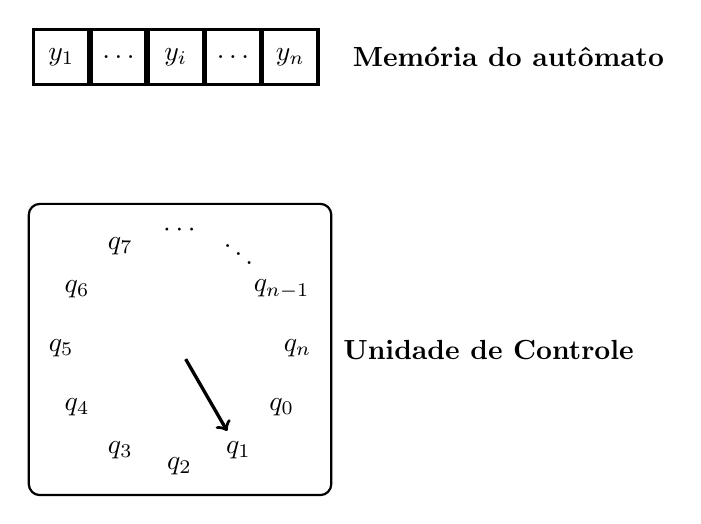
\begin{tikzpicture}
		\tikzstyle{every path}=[very thick]
		
		\edef\sizetape{0.7cm}
		\tikzstyle{tmtape}=[draw,minimum size=\sizetape]
		\tikzstyle{tmhead}=[arrow box,draw,minimum size=.5cm,arrow box
		arrows={east:.25cm, west:0.25cm}]
		
		%% Fita
		\begin{scope}[start chain=1 going right,node distance=-0.15mm]
			\node [on chain=1,tmtape] (input) {$y_1$};
			\node [on chain=1,tmtape] (raiz1) {$\ldots$};
			\node [on chain=1,tmtape] (alvo)  {$y_i$};
			\node [on chain=1,tmtape] (raiz2) {$\ldots$};
			\node [on chain=1,tmtape] (output){$y_n$};
			\node [on chain=1,xshift=0.3cm]        (descr) {\textbf{Memória do autômato}};
		\end{scope}
		
		%% Unidade de Controle
		\begin{scope}
			[shift={(1.5cm,-3.7cm)},start chain=circle placed {at=(-\tikzchaincount*30:1.5)}]
			%\foreach \i in {q_0,p_1,q_2,q_3, q_4,\ddots,q_n}
			\foreach \i in {q_0,q_1, q_2,q_3, q_4,q_5, q_6,q_7, \cdots,\ddots, q_{n-1},q_n}
			\node [on chain] {$\i$};
			
			% Seta para estado corrente
			\node (center) {};
			\draw[->] (center) -- (circle-2);
			
			\node[rounded corners,draw=black,thick,fit=(circle-1) (circle-2) (circle-3) 
			(circle-4) (circle-5) (circle-6) (circle-7) (circle-8) 
			(circle-9) (circle-10) (circle-11) (circle-12),
			label=right:\textbf{Unidade de Controle}] (fsbox)
			{};
		\end{scope}
		
		%% Draw TM head below (input) tape cell
		\node [draw=white, thick, yshift=-.3cm] at (alvo.south)   (head3) {};
		
		
	\end{tikzpicture}
	\caption{Informal do conceito de autômato finito com uma única memória retirado de \cite{valdi2020phd}.}
	\label{fig:AF-Informal}
\end{figure}

Formalmente pode-se dizer como apontado em \cite{valdi2020phd}, que a teoria dos autômatos finitos, ou simplesmente teoria dos autômatos, teve seu desenvolvimento inicial entre os anos de 1940 e 1960 sendo este início os trabalhos de McCulloch e Pitts \cite{mcculloch1943}, Kleene \cite{kleene1951}, Mealy \cite{mealy1955}, Moore \cite{moore1956}, Rabin e Scott \cite{rabin1963, rabin1959}. De forma geral os autômatos finitos são os mais simples modelos abstratos de máquinas de computação \cite{farias2017}, sendo eles máquinas de Turing limitadas. 

\section{Noções Fundamentais}\label{sec:Nocoesbasicas}

Neste primeiro momento para o estudo dos autômatos finitos serão apresentados alguns conceitos fundamentais de extrema importância para o desenvolvimento das próximas seções e capítulos.

\begin{definition}[Alfabetos e Palavras]\label{def:AlfabetoPalavra}
	Qualquer conjunto finito e não vazio $\Sigma$ será chamado de alfabeto. Qualquer sequência finita de símbolos na forma $a_1\cdots a_n$ com $a_i \in \Sigma$ para todo $1 \leq i \leq n$ será chamada de palavra sobre o alfabeto $\Sigma$.
\end{definition}

\begin{example}
	Os conjuntos $\{0, 1, 2, 3\}, \{a, b, c\}, \{\heartsuit,\spadesuit, \Diamond, \clubsuit\}$ e $\{n \in \mathbb{N} \mid n \leq 25\}$ são todos alfabetos, os conjuntos $\mathbb{N}$ e $\mathbb{R}$ não são alfabetos.
\end{example}

\begin{example}
	Dado o alfabeto $\Sigma = \{0, 1, 2, 3\}$ tem-se que as sequências 0123, 102345, 1 e 0000 são todas palavras sobre $\Sigma$.
\end{example}

\begin{definition}[Comprimento das palavras]\label{def:ComprimentoPalavra}
	Seja $w$ uma palavra qualquer sobre um certo alfabeto $\Sigma$, o comprimento\footnote{Por conta desta notação em alguns texto é usado o termo módulo em vez de comprimento.} de $w$, denotado por $|w|$, corresponde ao número de símbolos existentes em $w$.
\end{definition}

\begin{example}
	Dado o alfabeto $\Sigma = \{a, b, c, d\}$ e as palavras $abcd, aacbd, c$ e $ddaacc$ tem-se que: $|abcd| = 4, |aa| = 2, |c| = 1$ e $|ddaacc| = 6$.
\end{example}

\begin{remark}
	Em especial quando $|w| = 1$, é dito que $w$ é uma palavra unitária, isto é, a mesma contém apenas um único símbolo do alfabeto.
\end{remark}

Como muito bem explicado em \cite{benjaLivro2010, hopcroft2008, linz2006}, pode-se definir uma série de operações sobre palavras, sendo a primeira delas  a noção de concatenação.

\begin{definition}[Concatenação de palavras]\label{def:Concatenacao}
	Sejam $w_1 = a_1\cdots a_m$ e $w_2 = b_1\cdots b_n$ duas palavras quaisquer, tem-se que a concatenação de $w_1$ e $w_2$, denotado por $w_1w_2$, corresponde a uma sequência iniciada com os símbolos que forma $w_1$ imediatamente seguido dos símbolos que forma $w_2$, ou seja, $w_1w_2 = a_1\cdots a_mb_1\cdots b_n$.
\end{definition}

\begin{remark}
	O leitor deve ficar atento ao fato de que a concatenação apenas combina duas palavras em uma nova palavra, sendo que, não a qualquer tipo de exigência sobre os alfabeto sobre os quais as palavras usadas na concatenação estão definidas.
\end{remark}

\begin{example}\label{exe:Concatenacao}
	Dado duas palavras $w_1 = abra$ e $w_2 = cadabra$ tem-se que $w_1w_2 = abracadabra$ e $w_2w_1 = cadabraabra$.
\end{example}

Note que o Exemplo \ref{exe:Concatenacao} estabelece que a operação de concatenação entre duas palavras não é comutativa, isto é, a ordem com que as palavras aparecem na concatenação é responsável pela forma da palavra resultante da concatenação.

\begin{theorem}[Associativade da Concatenação]\label{teo:AssociatividaeConcatenacao}
	Para quaisquer $w_1, w_2$ e $w_3$ tem-se que $(w_1w_2)w_3 = w_1(w_2w_3)$.
\end{theorem}

\begin{proof}
	Dado três palavras quaisquer $w_1 = a_1\cdots a_i, w_2 = b_1\cdots b_j$ e $w_3 = c_1\cdots c_k$ tem-se que,
	\begin{eqnarray*}
		(w_1w_2)w_3 & = & (a_1\cdots a_ib_1\cdots b_j)c_1\cdots c_k\\
		& = & a_1\cdots a_ib_1\cdots b_jc_1\cdots c_k\\
		& = & a_1\cdots a_i(b_1\cdots b_jc_1\cdots c_k)\\
		& = & w_1(w_2w_3)
	\end{eqnarray*}
	o que conclui a prova.
\end{proof}

Sobre qualquer alfabeto $\Sigma$ sempre é definida uma palavra especial chamada \textbf{palavra vazia} \cite{hopcroft2008, linz2006}, esta palavra especial não possui nenhum símbolo, e em geral é usado o símbolo $\lambda$ para denotar a palavra vazia \cite{benjaLivro2010, valdi2016master}. Como mencionado em \cite{benjaLivro2010, valdi2020phd} sobre a palavra vazia é importante destacar que:

\begin{eqnarray}
	w\lambda & = & \lambda w = w\\
	|\lambda| & = &  0
\end{eqnarray}

Isto é, a palavra vazia é neutra para a operação de concatenação, além disso, a mesma apresenta comprimento nulo.

\begin{definition}[Potência das palavras]\label{def:PotenciaPalavras}
	Seja $w$ uma palavra sobre um alfabeto $\Sigma$ a potência de $w$ é definida recursivamente para todo $n \in \mathbb{N}$ como sendo:
	\begin{eqnarray}
		w^0 & = & \lambda\\
		w^{n+1} & = & ww^{n}
	\end{eqnarray}
\end{definition}

\begin{example}
	Sejam $w_1 = ab, w_2 = bac$ e $w_3 = cbb$ palavras sobre $\Sigma = \{a, b, c\}$ tem-se que:
	\begin{itemize}
		\item[(a)] $w_1^3 = w_1w_1^2 = w_1w_1w_1^1 = w_1w_1w_1w_1^0 = w_1w_1w_1\lambda = ababab$.
		\item[(b)] $w_2^2 = w_2w_2^1 = w_2w_2w_2^0 = w_2w_2\lambda = w_2w_2 = bacbac$.
	\end{itemize} 
\end{example}

\begin{example}
	Seja $u = 01$ e $v = 231$ tem-se que: 
	$$uv^3 = uvv^2 = uvvv^1 = uvvv\lambda = uvvv = 01231231231$$
	e também 
	$$u^2v = uu^1v = uu\lambda v = uuv = 0101231$$
\end{example}

\begin{proposition}
	Para toda palavra $w$ e todo $m,n \in \mathbb{N}$ tem-se que:
	\begin{itemize}
		\item[(i)] $(w^m)^n = w^{mn}$.
		\item[(ii)] $w^mw^n = w^{m+n}$.
	\end{itemize}
\end{proposition}

\begin{proof}
	Direto das Definições \ref{def:Concatenacao} e \ref{def:PotenciaPalavras}, e portanto, ficará como exercício ao leitor.
\end{proof}

%Outro importante conceito existente sobre a ideia de palavra é a noção de palavra inversa (ou reversa) formalmente definida como se segue.

\begin{definition}[Palavra Inversa]\label{def:PalavraInversa}
	\cite{valdi2016master} Seja $w = a_1\cdots a_n$ uma palavra qualquer, a palavra inversa de $w$ denotada por $w^r$, é tal que $w^r = a_n\cdots a_1$. 
\end{definition}

\begin{example}
	Dado as palavras $u = aba, v = 011101$ e $w = 3021$ tem-se que $u^r = aba, v^r = 101110$ e $w^r = 1203$.
\end{example}

\begin{remark}
	Com respeito a noção de palavra inversa tem-se em particular que vale a seguinte igualdade $\lambda^r = \lambda$.
\end{remark}

Além das palavras, pode-se também formalizar uma série de operações sobre a própria noção de alfabeto. Em primeiro lugar, uma vez que,  alfabetos são conjuntos, obviamente todas operações usuais de união, interseção, complemento, diferença e diferença simétrica (ver Capítulo \ref{cap:Conjuntos}) também são válidas sobre alfabetos. Além dessas operações, também esta definida a operação de potência e os fechos positivo e de Kleene sobre alfabetos.

\begin{definition}[Potência de um alfabeto]\label{def:PotenciaAlfabeto}
	\cite{benjaLivro2010} Seja $\Sigma$ um alfabeto a potência de $\Sigma$ é definida recursivamente para todo $n \in \mathbb{N}$ como:
	\begin{eqnarray}
		\Sigma^0 & = & \{\lambda\}\\
		\Sigma^{n+1} & = & \{aw \mid a \in \Sigma, w \in \Sigma^{n}\}
	\end{eqnarray}
\end{definition} 

\begin{example}
	Dado $\Sigma = \{a, b\}$ tem-se que $\Sigma^3 = \{aaa, aab, aba, baa, abb, bab, bba, bbb\}$ e $\Sigma^1 = \{a, b\}$
\end{example}

\begin{example}
	Seja $\Sigma = \{0, 1, 2\}$ tem-se que $\Sigma^2 = \{00, 01, 02, 10, 11, 12, 20, 21, 22\}$ e $\Sigma^{0} = \{\lambda\}$.
\end{example}

O leitor mais atencioso e maduro matematicamente pode notar que para qualquer que seja $n \in \mathbb{N}$ o conjunto potência tem a propriedade de que todo $w \in \Sigma^n$ é tal que $|w| = n$, além disso, é claro que todo $\Sigma^n$ é sempre finito\footnote{Essa afirmação é facilmente verificável, uma vez que, a mesma nada mais é do que um exemplo de arranjo com repetição.}.

\begin{definition}[Fecho Positivo e de Kleene]\label{def:FechoPositivoKleene}
	Seja $\Sigma$ um alfabeto o fecho positivo e o fecho de Kleene de $\Sigma$, denotados respectivamente por $\Sigma^+$ e $\Sigma^*$, correspondem aos conjuntos:
	\begin{eqnarray}
		\Sigma^+ & = & \bigcup_{i = 1}^\infty \Sigma^i
	\end{eqnarray}
	e
	\begin{eqnarray}
		\Sigma^* & = & \bigcup_{i = 0}^\infty \Sigma^i
	\end{eqnarray}
\end{definition}

Obviamente como dito em \cite{benjaLivro2010}, o fecho de positivo pode ser reescrito em função do fecho de Kleene usando a operação de diferença de conjunto, isto é, o fecho positivo corresponde a seguinte identidade, $\Sigma^+ = \Sigma^* - \{\lambda\}$. Sobre o fecho de Kleene com destacado em \cite{valdi2020phd} o mesmo corresponde ao monoide livremente\footnote{Relembre que uma álgebra é livremente gerada quando todo elemento possui fatoração única (a menos de isomorfismo).} gerado pelo conjunto $\Sigma$ munida da operação de concatenação.

\begin{definition}[Prefixos e Sufixos]\label{def:PrefixoSufixo}
	Uma palavra $u \in \Sigma^*$ é um prefixo de outra palavra $w \in \Sigma^*$, denotado por $u \preceq_p w$, sempre que $w = uv$, com $v \in \Sigma^*$. Por outro lado, uma palavra $u$ é um sufixo de outra palavra $w$, denotado por $u \preceq_s w$, sempre que $w = vu$.
\end{definition}

\begin{example}
	Seja $w = abracadabra$ tem-se qu~e as palavras $ab$ e $abrac$ são prefixos de $w$, por outro, lado $cadabra$ e $bra$ são sufixos de $w$, e a palavra $abra$ é prefixo e também sufixo. Já a palavra $cada$ não é prefixo e nem sufixo de $w$.
\end{example}

\begin{definition}[Conjunto dos Prefixos e Sufixos]\label{def:ConjuntoPrefixoSufixo}
	Seja $w \in \Sigma^*$ o conjunto de todos os prefixos de $w$ corresponde ao conjunto:
	\begin{eqnarray}
		PRE(w) = \{w' \in \Sigma^* \mid w' \preceq_p w\}
	\end{eqnarray}
	e o conjunto de todos os sufixos de $w$ corresponde ao conjunto:
	\begin{eqnarray}
		SUF(w) = \{w' \in \Sigma^* \mid w' \preceq_s w\}
	\end{eqnarray}
\end{definition}

\begin{example}
	Seja $w = univasf$ tem-se que:
	\begin{eqnarray*}
		PRE(w) = \{\lambda, u, un, uni, univ, univa, univas, univasf\}
	\end{eqnarray*}
	e
	\begin{eqnarray*}
		SUF(w) = \{\lambda, f, sf, asf, vasf, ivasf, nivasf, univasf \}
	\end{eqnarray*}
\end{example}

\begin{example}
	A seguir é apresentado alguns exemplos de palavras e seus conjuntos de prefixos e sufixos.
	\begin{itemize}
		\item[(a)] Se $w = ab$, então $PRE(w) = \{\lambda, a, ab\}$ e  $SUF(w) = \{\lambda, b, ab\}$.
		\item[(b)] Se $w = 001$, então $PRE(w) = \{\lambda, 0, 00, 001\}$ e  $SUF(w) = \{\lambda, 1, 01, 001\}$.
		\item[(c)] Se $w = \lambda$, então $PRE(w) = \{\lambda\}$ e  $SUF(w) = \{\lambda\}$
		\item[(d)] Se $w = a$, então $PRE(w) = \{\lambda, a\}$ e $SUF(w) = \{\lambda, a\}$.
	\end{itemize}
\end{example}

Com respeito a cardinalidade dos conjuntos de prefixos e sufixos, os mesmo apresentam as propriedades descritas pelo teorema a seguir.

\begin{theorem}\label{teo:CardinalidadePrefixoSufixo}
	Para qualquer que seja $w \in \Sigma^*$ as seguintes asserções são verdadeiras.
	\begin{itemize}
		\item[(i)] $\# PRE(w) = |w| + 1$.
		\item[(ii)] $\#PRE(w) = \#SUF(w)$.
		\item[(iii)] $\#(PRE(w) \cap SUF(w)) \geq 1$.
	\end{itemize}
\end{theorem}

\begin{proof}
	Dado uma palavra $w$ tem-se que:
	\begin{itemize}
		\item[(i)] Sem perda de generalidade assumindo que $w = a_1\cdots a_n$ logo $w \in \Sigma^n$ (o caso quando $w = \lambda$ é trivial e não será demonstrado aqui) logo $|w| = n$ para algum $n \in \mathbb{N}$, assim existem exatamente $n$ palavras da forma $a_1 \cdots a_i$ com $1 \leq i \leq n$ tal que $a_1 \cdots a_i \preceq_p w$, portanto, para todo $1 \leq i \leq n$ tem-se que $a_1 \cdots a_i \in PRE(w)$, além disso, é claro que $w = \lambda w$, e portanto, $\lambda \in PRE(w)$, consequentemente, $\#PRE(w) = n + 1 = |w| + 1$.
		\item[(ii)] É suficiente mostrar que $\# SUF(w) = |w| + 1$, para isso como antes sem perda de generalidade assuma que $w = a_1\cdots a_n$ e assim tem-se que $w \in \Sigma^n$ logo $|w| = n$ com $n \in \mathbb{N}$, dessa forma existem exatamente $n$ palavras da forma $a_i \cdots a_n$ com $1 \leq i \leq n$ tal que $a_i \cdots a_n \preceq_s w$, portanto, para todo $1 \leq i \leq n$ tem-se que $a_i \cdots a_n \in SUF(w)$, além disso, é claro que $w = w\lambda$, logo $\lambda \in SUF(w)$, consequentemente, $\#SUF(w) = n + 1 = |w| + 1$, e portanto, $\#PRE(w) = \#SUF(w)$. O caso $w = \lambda$ é trivial e não será demonstrado aqui.
		\item[(iii)] Trivial, pois basta notar que $\lambda \in (PRE(w) \cap SUF(w))$, e portanto, tem-se claramente que $\#(PRE(w) \cap SUF(w)) \geq 1$.
	\end{itemize}
\end{proof}

\begin{corollary}
	Toda palavra tem pelo menos um prefixo e um sufixo.
\end{corollary}

\begin{proof}
	Direto do item $(iii)$ do Teorema \ref{teo:CardinalidadePrefixoSufixo}.
\end{proof}

Seguindo com o texto deste manuscrito pode-se finalmente formalizar o pilar fundamental (a ideia de linguagem) necessário para desenvolver o estuda da computabilidade neste e nos próximo capítulos.

\begin{definition}[Linguagem]\label{def:Linguagem}
	Dado um alfabeto $\Sigma$, qualquer subconjunto $L \subseteq \Sigma^*$ será chamado de linguagem.
\end{definition}

\begin{example}
	Seja $\Sigma = \{0, 1\}$ tem-se que os conjuntos a seguir são todos linguagens sobre $\Sigma$.
	\begin{itemize}
		\item[(a)] $\Sigma^*$.
		\item[(b)] $\{0^nb^n \mid n \in \mathbb{N}\}$.
		\item[(c)] $\{\lambda, 0, 1\}$.
		\item[(d)] $\Sigma^{22}$.
		\item[(e)] $\emptyset$.
	\end{itemize}
\end{example}

Similarmente ao que ocorre com os alfabetos, as linguagens por serem conjuntos ``herdam'' as operações básicas da teoria dos conjuntos \cite{lipschutz1978-TC, lipschutz2013-MD, abe1991-TC}, isto é, estão definidas sobre as linguagens as operações de união, interseção, completo, diferença e diferença simétrica. E como par aos alfabetos novas operações são definidas.

\begin{definition}[Concatenação de Linguagens]\label{def:ConcatenacaoLinguagem}
	Sejam $L_1$ e $L_2$ duas linguagens, a concatenação de $L_1$ com $L_2$, denotado por $L_1L_2$, corresponde a seguinte linguagem:
	\begin{eqnarray}
		L_1L_2 = \{xy \in (\Sigma_1 \cup \Sigma_2)^* \mid x \in L_1, y \in L_2\}
	\end{eqnarray}
\end{definition}

\begin{example}\label{exe:ConcatenacaoLinguagem} 
	Dado as três linguagens $L_1 = \{\lambda, ab, bba\}, L_2 =\{0^{2n}1 \mid n \in \mathbb{N}\}$ e $L_3 = \{a^p \mid p \text{ é primo}\}$ tem-se que:
	\begin{itemize}
		\item[(a)] $L_1L_2 = \{w \mid w = 0^{2n}1 \text{ ou } w = ab0^{2n}1 \text{ ou } w = bba0^{2n}1 \text{ com } n \in \mathbb{N}\}$.
		\item[(b)] $L_3L1 = \{w \mid w = a^p \text{ ou } w = a^{p+1}b \text{ ou } a^pbba \text{ onde } p \text{ é um número primo}\}$.
		\item[(c)] $L_2L_3 = \{0^{2n}1a^p \mid n \in \mathbb{N}, p \text{ é um número primo}\}$.
	\end{itemize}
\end{example}

\begin{definition}[Linguagem Reversa]\label{def:LinguagemReversa}
	Seja $L$ uma linguagem, a linguagem inversa de $L$, denotada por $L^r$, corresponde ao conjunto $\{w^r \mid w \in L\}$.
\end{definition}

\begin{example}
	Considerando as linguagens $L_1, L_2$ e $L_3$ do Exemplo \ref{exe:ConcatenacaoLinguagem} e a linguagem $\{01, 011\}$ tem-se que:
	\begin{itemize}
		\item[(a)] $L_1^r = \{\lambda, ba, abb\}$.
		\item[(b)] $L_2^r = \{10^{2n} \mid n \in \mathbb{N}\}$.
		\item[(c)] $L_3^r = \{a^p \mid n \in \mathbb{N}, p \text{ é um número primo}\}$.
		\item[(d)] $\{01, 011\}^r = \{10, 110\}$.
	\end{itemize}
\end{example}

O leitor mais atento pode perceber que a propriedade involutiva da operação reversa sobre palavras é ``herdada'' para a reversão sobre linguagens, isto é, para qualquer linguagem $L$ tem-se que $(L^r)^r = L$. 

\begin{definition}[Linguagem Potência]
	Seja $L$ uma linguagem, a linguagem potência de $L$, denotada por $L^n$, é definida recursivamente para todo $n \in \mathbb{N}$ como:
	\begin{eqnarray}
		L^0 & = &\{\lambda\}\\
		L^{n+1} & = &  LL^{n}
	\end{eqnarray}
\end{definition}

Utilizando o conceito de linguagem potência a seguir é apresentado a formalização para os fechos positivo e de Kleene sobre linguagens.

\begin{definition}[Fecho positivo e Fecho de Kleene de Linguagens]\label{def:FechoPositivoKleeneLinguagem}
	Seja $L$ uma linguagem, o fecho positivo $(L^+)$ e o fecho de Kleene $(L^*)$ de $L$ são dados pelas equações a seguir.
	\begin{eqnarray}
		L^+ & = & \bigcup_{i = 1}^\infty L^i\\
		L^* & = & \bigcup_{i = 0}^\infty L^i
	\end{eqnarray}
\end{definition}

Por fim, esta seção irá apresentar a noção de linguagem dos prefixos e sufixos.

\begin{definition}[Linguagem de Prefixos e Sufixos]\label{def:LinguagemPrefixosSufixos}
	Seja $L$ uma linguagem, a linguagem dos prefixos e dos sufixos de $L$, respectivamente $PRE(L)$ e $SUF(L)$, são exatamente os seguintes conjuntos:
	\begin{eqnarray*}
		PRE(L) & = & \{w' \in \Sigma^* \mid w' \preceq_p w, w \in L\}\\
		SUF(L) & = & \{w' \in \Sigma^* \mid w' \preceq_s w, w \in L\}
	\end{eqnarray*}
\end{definition}

\begin{example}
	Considere a linguagem $\{0, 10, 11010\}$ tem-se que:
	\begin{eqnarray*}
		PRE(\{0, 10, 11010\}) & = & \{\lambda, 0, 1, 10, 11, 110, 1101, 11010\}\\
		SUF(\{0, 10, 11010\}) & = & \{\lambda, 0, 10, 010, 1010, 11010\}
	\end{eqnarray*}
\end{example}

Nos próximos capítulos deste manuscrito irão ser apresentadas as formalizações da ideia de linguagens formais na visão ``mecânica'' de Turing \cite{turing1937}, entretanto, em vez de apresentar de forma direta os conceitos ligados as máquinas de Turing e as computações por elas realizadas, este manuscrito opta por fazer um estudo seguindo a ideia dos livros texto de linguagens formais \cite{benjaLivro2010, linz2006, menezes1998LFA}, assim sendo, este parte do manuscrito irá apresentar as linguagens formais da mais simples para a mais complexas seguindo a hierarquia de Chomsky \cite{chomsky1956}, ou seja, serão aqui estudadas as linguagens formais na seguintes ordem: regulares, livres do contexto, recursivas e recursivamente enumeráveis.

\section{Sobre Gramática Formais}\label{sec:GramaticaFormal}

Agora que foram introduzidos os conceitos fundamentais para a teoria das linguagens formais pode-se formalizar o conceito de estrutura geradora ou gramática formal, o leitor mais atento e com maior conhecimento sobre lógica de primeira ordem e teoria da prova \cite{avigad1998, buss1998} pode notar que gramáticas formais são na verdade outro nome para  sistemas de reescrita \cite{ayala2014}.

\begin{definition}[Gramática formal]\label{def:GramaticaFormal}
	Uma gramática formal é uma estrutura da forma $G = \langle V, \Sigma, S, P \rangle$ onde $V$ é um conjunto não vazio de símbolos chamados variáveis tal que $V \cap \Sigma = \emptyset$, $\Sigma$ é um alfabeto, $S \in V$ é uma variável destacada chamada de \textbf{variável inicial} e $P$ é um conjunto de regras de reescrita\footnote{Tamém é comum encontrar na literatura a nomenclatura regras de produção \cite{benjaLivro2010, linz2006}.} da forma $w \rhd w'$ onde $w \in (V \cup \Sigma)^+$ e $w' \in (V \cup \Sigma)^*$.
\end{definition}

\begin{example}\label{exe:GramaticaFormal1} 
	A estrutura $G = \langle \{A, B\}, \{a\}, A, P \rangle$ em que $P$ é formado pelas regras $A \rhd aABa, A \rhd B$ e $B \rhd \lambda$ é uma gramática formal.
\end{example}

Qualquer gramática então pode ser visto com um sistema para a geração de palavras através de um mecanismo chamado derivação descrito a seguir.

\begin{definition}[Derivação de palavras]
	Dado uma gramática $G = \langle V, \Sigma, S, P \rangle$, a palavra $XwY$ deriva a palavra $Xw'Y$  na gramática $G$, denotado por $XwY \gg_G Xw'Y$, sempre que existe uma regra forma $w \rhd w' \in P$.
\end{definition}

\begin{example}
	Dado a gramática do Exemplo \ref{exe:GramaticaFormal1} tem-se que $aABa \gg_G aaABaBa$, pois existe em $P$ a regra $A \rhd aABa$.
\end{example}

Rigorosamente $\gg_G$ na verdade é uma relação entre $(V \cup \Sigma)^+$ e $(V \cup \Sigma)^*$, e assim $\gg_G^*$ denota o fecho transitivo e reflexivo de  $\gg_G$, além disso, sempre que não causar confusão é comum eliminar a escrita do rótulo da gramática, ou seja, são escritos respectivamente $\gg^*$ e $\gg$ em vez de $\gg_G^*$ e $\gg_G$.

\begin{example}
	Considerando ainda a gramática exibida no Exemplo \ref{exe:GramaticaFormal1} tem-se que $aABa \gg^* aaaABaBaBa$, uma vez que, $aABa \gg aaABaBa \gg aaaABaBaBa$.
\end{example}

\begin{example}
	A estrutura $G = \langle \{A, B, S\}, \{0,1\}, S, P \rangle$ em que $P$ é formado pelas regras $S \rhd 11A, A \rhd B0$ e $B \rhd 000$ é uma gramática formal e assim $11A \gg^* 110000$, pois tem-se que, $11A \gg^* 11B0 \gg^* 110000$.
\end{example}

Como dito em \cite{benjaLivro2010}, dado uma gramática formal $G$ tem-se que sempre houver uma sequencia de derivações $w_1 \gg w_2 \gg \cdots \gg w_n$ acontecer, as palavras $w_1, w_2, \cdots, w_n$ são chamadas de formas sentenciais, ou simplesmente, sentenças. Assim uma derivação nada mais é do que uma sequência finita de formas sentenciais.

\begin{definition}[Igualdade de Derivações]\label{def:IgualdadeDerivacaoGramatica}
	Dado uma gramática $G = \langle V, \Sigma, S, P \rangle$ e duas derivações $S \gg w_1 \gg^* w_n$ e $S \gg w'_1 \gg^* w'_n$ sobre $G$, será dito que estas derivações são iguais sempre que $w_i = w'_i$ para todo $1 \leq i \leq n$.
\end{definition}

Desde que $\gg^*$ é de fato uma relação pode-se facilmente que a igualdade entre derivações nada mais é do que a igualdade entre tuplas ordenadas.

\begin{definition}[Linguagem de uma gramática]\label{def:LinaugemGramatica}
	Dado uma gramática $G = \langle V, \Sigma, S, P \rangle$ a linguagem gerada por $G$, denotada por $\mathcal{L}(G)$, corresponde ao conjunto formado por todas as palavras sobre $\Sigma$ que são deriváveis a partir do variável inicial da gramática, ou seja, $\mathcal{L}(G) = \{w \in \Sigma^* \mid S \gg^* w\}$.
\end{definition}

\begin{example}
	Não é difícil verificar que a gramática do Exemplo \ref{exe:GramaticaFormal1} gera a linguagem $\{w \in \{a\}^* \mid |w| = 2k, k \in \mathbb{N}\}$.
\end{example}

Agora o leitor pode ter notado que como gramática formais possuem um conjunto finito de regras, as linguagens por elas geradas nada mais são do que conjuntos indutivamente gerados.

\begin{problemset}
	\item Dado o alfabeto $\Sigma = \{a, b, c\}$ e as palavras $u = aabcab, v = bbccabac$ e $w = ccbabbaaca$ determine:
	\begin{enumerate}
		\item A palavra $uv^r$.
		\item A palavra $(w^r)^2u$.
		\item A palavra $((u^r)^2v^0)^rv$.
		\item A palavra $uu^2v^rw$.
		\item A palavra $((wuv)^r)^2u$.
		\item O valor da expressão $|w^3| + 2|v^2u| - |u|$.
		\item O valor da expressão $2|w^r| - |uv|$.
		\item O valor da expressão $|w^raaw| - |w|$.
		\item O valor da expressão $|uv^r| - 4$.
		\item O valor da expressão $\frac{|(w^r)^2u|}{2} - \frac{|u|}{6}$.
	\end{enumerate}
	\item Demonstre para quaisquer palavras $u$ e $v$ e para todo $n \in \mathbb{N}$ as asserções a seguir.
	\begin{enumerate}
		\item Se $u$ é um prefixo de $v$, então $|u| \leq |v|$.
		\item $|u^n| = n|u|$.
		\item $|(uv)^r| = |vu|$.
		\item Se $|u| = n$, então $n \leq |uv|$.
	\end{enumerate}
	\item Considere a linguagem $L = \{\lambda, abb, a, abba\}$ e determine:
	\begin{enumerate}
		\item $L^r - \{\lambda, a\}$.
		\item $L^3$.
		\item $PRE(L)$.
		\item $SUF(L^2)$.
		\item $w$ tal que $|w| = \bigsqcup \{|w'| \mid w' \in L^3\}$.
	\end{enumerate}
	\item Prove que para qualquer linguagem $L$ e quaisquer $m,n \in \mathbb{N}$ as seguintes asserções.
	\begin{enumerate}
		\item $(L^m)^n = L^{mn}$.
		\item $L^mL^n = L^{m+n}$.
		\item $(L^r)^n = (L^n)^r$.
		\item $\overline{L}^r = \overline{L^r}$.
		\item $PRE(L) = (SUF(L^r))^r$.
	\end{enumerate}
	\item Dado duas linguagens quaisquer $L_1$ e $L_2$ demostre que:
	\begin{enumerate}
		\item Se $L_1 \cap L_2 \neq \emptyset$, então $PRE(L_1) \cap PRE(L_2) = \emptyset$.
		\item Se $L_1 \subseteq L_2$, então $SUF(L_1) \cap SUF(L_2) = \emptyset$.
		\item Se $L_1 \subseteq L_2$, então $L_1^r \subseteq L_2^r$.
		\item Se $L_1 \subseteq L_2$, então para todo $L$ tem-se que $LL_1 \subseteq LL_2$. 
	\end{enumerate}
	\item Demonstre ou refute o predicado $(\forall L \subseteq \Sigma^*)[(\forall n \in \mathbb{N})[\overline{L}^n = \overline{L^n}]]$.
	\item Esboce formalmente em que condições a igualdade $PRE(L) = (SUF(L))^r$ é verdadeira.
\end{problemset}
	\chapter{Linguagens Regulares}\label{cap:LinguagemRegulares}

\begin{introduction}[Conteúdos]
	\item Autômatos Finitos Determinísticos
	\item Autômatos Finitos Não-determinísticos
	\item $\lambda$-Autômatos Finitos Não-determinísticos
	\item Teorema Myhill-Nerode e a  minimização
	\item Máquinas de Mealy e Moore
	\item Notação Matricial
	\item Expressões Regulares
	\item Gramáticas Regulares
	\item Álgebra das Linguagens Regulares
	\item Questionário
\end{introduction}

\section{Autômato Finito Determinístico}\label{sec:AFD}

Como explicado em diversas obras tais como \cite{benjaLivro2010, hopcroft2008, linz2006, menezes1998LFA}, os autômatos finitos podem ser separados em dois tipos bem definidos, a saber Autômato Finito Determinístico (AFD) e Autômato Finito Não-determinístico (AFN). Agora este manuscrito inicia o estudo dos AFD apresentando sua forma algébrica equacional.

\begin{definition}[Autômato Finito Determinístico]\label{def:AFD}
	Um AFD é uma estrutura $A = \langle Q, \Sigma, \delta, q_0, F\rangle$ onde: $Q$ é um conjunto finito de estados, $\Sigma$ é um alfabeto, $\delta : Q \times \Sigma \rightarrow Q$ é uma função total (chamada função de transição), $q_0 \in Q$ é um estado destacado (chamado estado inicial) e $F \subseteq Q$ é o conjunto de estados finais\footnote{Em algumas referências também é usado o termo conjunto de estados de aceitação \cite{de2010}.}.
\end{definition}

\begin{example}\label{exe:AFD}
	A estrutura $A = \langle \{q_0, q_1\}, \{a\}, \delta, q_0, \{q_1\} \rangle$ onde a função de transição é definida por: $\delta(q_0, a) = q_1$ e $\delta(q_1, a) = q_0$, é um AFD.
\end{example}

\begin{example}\label{exe:NaoEAFD}
	A estrutura $B = \langle \{q_0, q_1, q_2\}, \{a, b\}, \delta, q_0, \{q_0\} \rangle$ onde a função de transição é definida por:
	\begin{table*}[h]
		\centering
		\begin{tabular}{ccc}
			$\delta(q_0, a) = q_1$ & $\delta(q_1, a) = q_2$ & $\delta(q_2, a) = q_1$\\
			$\delta(q_0, b) = q_1$ & $\delta(q_1, b) = q_2$ & 
		\end{tabular}
	\end{table*}

	\noindent não é um AFD, pois $\delta(q_2, b)$ não está definido, e portanto, $\delta$ não é uma função total furando assim a definição de AFD.
\end{example}

\begin{note}
	Para simplificar a escrita neste manuscrito as siglas AFD e AFN serão usado tanto para designar o singular quanto o plural, ficando a distinção a critério dos conectivos antes de cada sigla.
\end{note}

A função de transição $(\delta)$ pode ser interpretada semanticamente como sendo o programa que o autômato executa, assim uma aplicação qualquer de $\delta$ é uma instrução do programa do autômato, por exemplo, a aplicação $\delta(q, x) = p$ significa que, o AFD muda do estado atual $q$ para o estado $p$ quando o mecanismo de leitura lê o símbolo $x$ na memória. 

Uma representação comum para os AFD é baseada no uso de grafos de transição \cite{valdi2020phd}. Em um grafo de transição os vértices irão ser representados por círculos, que neste caso são usados para representar os estados do autômato, isto é, os círculos representam os elementos de $Q$. Cada aresta $(q_i, q_j)$ são rotuladas por $x$ representando assim a transição da forma $\delta(q_i, x) = q_j$. Por fim, os estados finais, isto é, cada $q \in F$ será representado por vértices desenhados como um círculo duplo em vez de um círculo simples e o estado inicial é marcado com uma seta.

\begin{example}\label{exe:AFDA}
	A representação por grafo de transição do AFD descrito no Exemplo \ref{exe:AFD} corresponde a figura a seguir.
	
	\begin{figure}[ht]
		\centering
		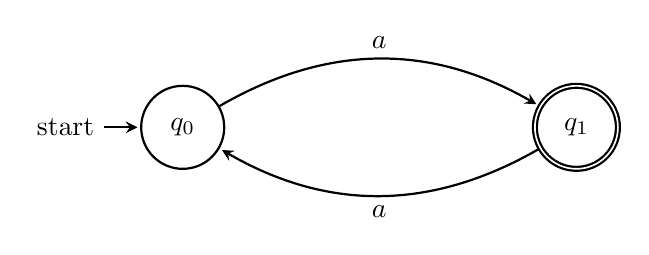
\begin{tikzpicture}[>=stealth, shorten >=1pt, node distance=5.0cm, on grid, auto, state/.append style={minimum size=3em}, thick ]
			\node[state, initial]   (A)               {$q_0$};
			\node[state, accepting] (B) [right of=A]  						 {$q_1$};
			
			\path[->] (A) +(-1,0) edge (A)
			
			%Transições:
			%(Partida) edge [tipo da seta] node {simbolo lido} (Destino)
			(A) edge [bend left]  				node {$a$}     		(B)
			(B) edge [bend left]  				node {$a$}     		(A);
		\end{tikzpicture}
		\caption{Representação visual do AFD no Exemplo \ref{exe:AFD}.}
		\label{fig:AFD}
	\end{figure}
\end{example}

\begin{example}\label{exe:AFDS}
	O AFD $S = \langle \{s_0, s_1, s_2\}, \{0,1\}, \delta, s_0, \emptyset \rangle$ onde a função de transição é definida como sendo: $\delta(s_0, 0) = s_1, \delta(s_1, 0) = s_2, \delta(s_2, 0) = s_1, \delta(s_0, 1) = s_2, \delta(s_1, 1) = s_1$ e $\delta(s_2, 1) = s_1$, é um AFD e pode ser representado pela Figura \ref{fig:AFD2} a seguir.
	
	\begin{figure}[h]
		\centering
		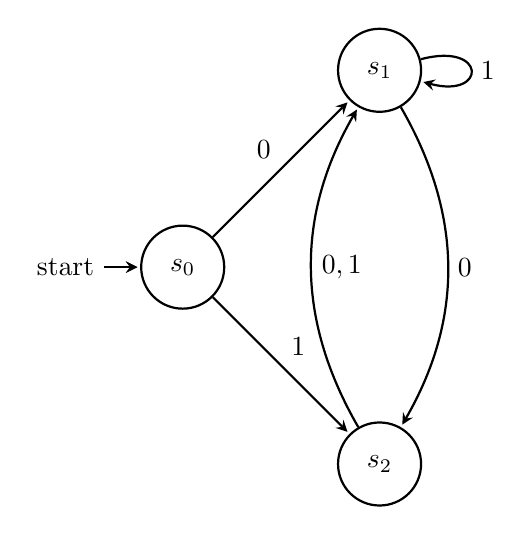
\begin{tikzpicture}[>=stealth, shorten >=1pt, node distance=2.5cm, on grid, auto, state/.append style={minimum size=3em}, thick ]
			\node[state, initial]   			(A)               {$s_0$};
			\node[]		  						(C) [right of=A]  {};
			\node[state] 						(B) [above of=C]  {$s_1$};
			\node[state] 						(D) [below of=C]  {$s_2$};
			
			\path[->] (A) +(-1,0) edge (A)
			
			%Transições:
			%(Partida) edge [tipo da seta] node {simbolo lido} (Destino)
			(B) edge [loop right]               node {$1$}           ( )
			(A) edge			  				node {$0$}     		 (B)
			(A) edge			  				node {$1$}     		 (D)
			(B) edge [bend left]  				node {$0$}     		 (D)
			(D) edge [bend left]  				node [right] {$0, 1$}(B);
		\end{tikzpicture}
		\caption{Representação visual do AFD $S$ do Exemplo \ref{exe:AFDS}.}
		\label{fig:AFD2}
	\end{figure}
\end{example}

Pode-se agora então estender a função de transição, para que o autômato possa vir a processar palavras, em vez de apenas símbolos individuais. 

\begin{definition}[Função de Transição Estendida]\label{def:DeltaEstendido}
	Seja $A = \langle Q, \Sigma, \delta, q_0, F\rangle$ um AFD a função $\delta$ é estendida para uma função $\widehat{\delta}: Q \times \Sigma^* \rightarrow Q$ usando recursividade como se segue.
	\begin{eqnarray}\label{eq:ExtensaoDaFuncaoTransicaoDelta}
		\widehat{\delta}(q, \lambda)& = & q \\
		\widehat{\delta}(q, wa)& = & \delta(\widehat{\delta}(q, w), a)	
	\end{eqnarray}
	onde $q \in Q, a \in \Sigma$ e $w \in \Sigma^*$.
\end{definition}

A partir da definição de função de transição estendida é definida  a noção de computação para os AFD, tal conceito é formalizado a seguir.

\begin{definition}[Computação em AFD]\label{def:ComputacaoAFD}
	Seja $A = \langle Q, \Sigma, \delta, q_0, F\rangle$ um AFD e seja $w \in \Sigma^*$ uma computação de $w$ em $A$ corresponde a aplicação $\widehat{\delta}(q_0, w)$.
\end{definition}

Note que a definição de computação em AFD pode ser interpretada como sendo a resposta ao seguinte questionamento: ``Em que estado o autômato (ou a máquina) estará após iniciar o processamento no estado inicial e ter lido todos os símbolos da palavra de entrada $w$?''

\begin{example}\label{exe:ComputacaoAFD1}
	Considere o AFD do Exemplo \ref{exe:AFD} e a palavra de entrada $aaaa$ tem-se que a computação desta palavra corresponde a:
	\begin{eqnarray*}
		\widehat{\delta}(q_0, aaaa) & = & \delta(\widehat{\delta}(q_0, aaa), a)\\
		& = & \delta(\delta(\widehat{\delta}(q_0, aa), a), a)\\
		& = & \delta(\delta(\delta(\widehat{\delta}(q_0, a), a), a), a)\\
		& = & \delta(\delta(\delta(\delta(\widehat{\delta}(q_0, \lambda), a), a), a), a)\\
		& = & \delta(\delta(\delta(\delta(q_0, a), a), a), a)\\
		& = & \delta(\delta(\delta(q_1, a), a), a)\\
		& = & \delta(\delta(q_0, a), a)\\
		& = & \delta(q_1, a)\\
		& = & q_0
	\end{eqnarray*}
\end{example}

\begin{example}\label{exe:ComputacaoAFD2}
	Considere o AFD do Exemplo \ref{exe:AFDS} e a palavra de entrada $0101$ tem-se que a computação desta palavra corresponde a:
	\begin{eqnarray*}
		\widehat{\delta}(s_0, 0101) & = & \delta(\widehat{\delta}(s_0, 010), 1)\\
		& = & \delta(\delta(\widehat{\delta}(s_0, 01), 0), 1)\\
		& = & \delta(\delta(\delta(\widehat{\delta}(s_0, 0), 1), 0), 1)\\
		& = & \delta(\delta(\delta(\delta(\widehat{\delta}(s_0, \lambda), 0), 1), 0), 1)\\
		& = & \delta(\delta(\delta(\delta(s_0, 0), 1), 0), 1)\\
		& = & \delta(\delta(\delta(s_1, 1), 0), 1)\\
		& = & \delta(\delta(s_1, 0), 1)\\
		& = & \delta(s_2, 1)\\
		& = & s_1
	\end{eqnarray*}
\end{example}

De pose da definição de computação pode-se formalizar o conceito de reconhecimento (ou aceitação) de palavras nos AFD.

\begin{definition}[Reconhecimento de palavras em AFD]\label{defi:PalavraAceitaPorAFD}
	\cite{benjaLivro2010} Sejam $A = \langle Q, \Sigma, \delta, q_0, F\rangle$ um AFD e seja $w \in \Sigma^*$. A palavra $w$ é dita aceita (reconhece ou computada) por $A$ sempre que $\widehat{\delta}(q_0, w) \in F$ e é rejeitada por $A$ em qualquer outro caso.
\end{definition}

É fácil perceber que $\widehat{\delta}(q_0, w) \in F$ com $w = a_1a_2\cdots a_n$ se, e somente se, existir uma sequência finita de estados $(q_i)_{i \in I}$ tal que $\delta(q_0, a_1) = q_{i_1}, \delta(q_{i_1}, a_2) = q_{i_2}, \cdots, \delta(q_{i_{n-1}}, a_{n}) = q_{i_n}$ com $q_n \in F, I$ sendo uma sequencia de números naturais e $i_1, i_2, i_{n-1}, i_n \in I$. O leitor pode notar que em particular tem-se que $\widehat{\delta}(q_0, \lambda) \in F$ se, e somente se, $q_0 \in F$.

\begin{example}\label{exe:AceiteAFD1}
	Considerando os Exemplos \ref{exe:ComputacaoAFD1} e \ref{exe:ComputacaoAFD2} tem-se que a palavra $aaaa$ não é aceita pelo AFD do Exemplo \ref{exe:ComputacaoAFD1}, uma vez que, $q_0 \notin F$. Já a palavra $0101$ também não é aceita pelo AFD do Exemplo \ref{exe:ComputacaoAFD2}, uma vez que, $s_1 \notin F$, de fato o leitor atento pode notar que o AFD do Exemplo \ref{exe:ComputacaoAFD2} não aceita qualquer palavra de entrada pois $F = \emptyset$.
\end{example}

\begin{remark}
	Note que se um AFD não aceitar qualquer palavra, é diferente de dizer que ele não realiza computação, pois como ja mencionado anteriormente uma computação é apenas a aplicação da função $\widehat{\delta}$, já não aceitar palavras diz respeito ao fato de $F = \emptyset$.
\end{remark}

\begin{example}\label{exe:AceiteAFD2}
	Considere o AFD representado pelo grafo de transições a seguir.
	
	\begin{figure}[h]
		\centering
		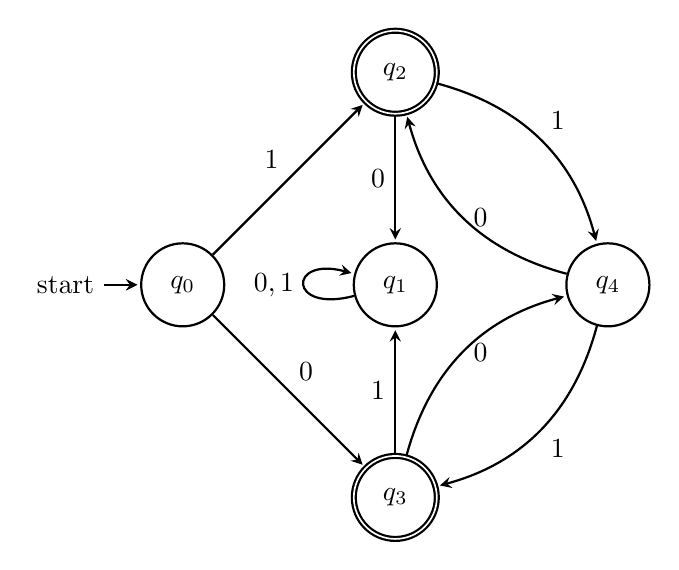
\begin{tikzpicture}[>=stealth, shorten >=1pt, node distance=2.7cm, on grid, auto, state/.append style={minimum size=3em}, thick ]
			\node[state, initial]   			(A)               {$q_0$};
			\node[state] 						(B) [right of=A]  {$q_1$};
			\node[state, accepting]				(C) [above of=B]  {$q_2$};
			\node[state, accepting]				(D) [below of=B]  {$q_3$};
			\node[state] 						(E) [right of=B]  {$q_4$};
			
			\path[->] (A) +(-1,0) edge (A)
			
			%Transições:
			%(Partida) edge [tipo da seta] node {simbolo lido} (Destino)
			(A) edge 				            node {$1$}           (C)
			(A) edge			  				node {$0$}     		 (D)
			(C) edge [bend left]  				node {$1$}     		 (E)
			(C)	edge							node [left] {$0$}	 (B)
			(E) edge [bend left]  				node [right] {$0$} 	 (C)
			(D) edge [bend left]  				node [right] {$0$}	 (E)
			(D)	edge							node [left] {$1$}	 (B)
			(E) edge [bend left]  				node {$1$} 	 		 (D)
			(B) edge [loop left]                node {$0,1$}         ( );
		\end{tikzpicture}
		\caption{Um AFD com dois estados finais.}
		\label{fig:AFD3}
	\end{figure}
	
	Por indução sobre o tamanho das palavras é fácil mostrar que este AFD reconhece palavras as palavras $1(10)^n1$ e $0(01)^n0$ com $n \in \mathbb{N}$.
\end{example}

Tendo definido precisamente as noções de AFD e de computação em AFD, agora é possível definir formalmente a ideia de linguagem reconhecida (ou computada) por um AFD.

\begin{definition}[Linguagem de um AFD]\label{def:LinguagemAFD}
	Seja $A = \langle Q, \Sigma, \delta, q_0, F\rangle$ um AFD a linguagem reconhecida (ou computada) por $A$, denotada por $\mathcal{L}(A)$, corresponde ao conjunto de todas as palavras aceitas por $A$, formalmente tem-se que:
	\begin{eqnarray}
		\mathcal{L}(A) = \{w \in \Sigma^* \mid \widehat{\delta}(q_0, w) \in F\}
	\end{eqnarray}
\end{definition}

Utilizando a definição acima o leitor deve ser capaz de perceber que se um AFD reconhece uma linguagem $L \subseteq \Sigma^*$, então ele para em estados finais apenas para as palavras $w \in L$. Em outra palavra para mostrar que uma linguagem $L$ é a linguagem de um AFD $A$, deve-se provar que $L = \mathcal{L}(A)$, ou seja, deve-se provar que $w \in L \Longleftrightarrow w \in \mathcal{L}(A)$, em geral quando $L$ é infinito tal prova é por indução.

\begin{example}\label{exe:AFDLinguagem1}
	A seguir você encontrará a prova de que a linguagem $L = \{bba^{2n} \mid n \in \mathbb{N}\}$ é reconhecida pelo AFD $A_1$ na Figura \ref{fig:AFDLinguagem1} a seguir. 
	\begin{figure}[h]
		\centering
		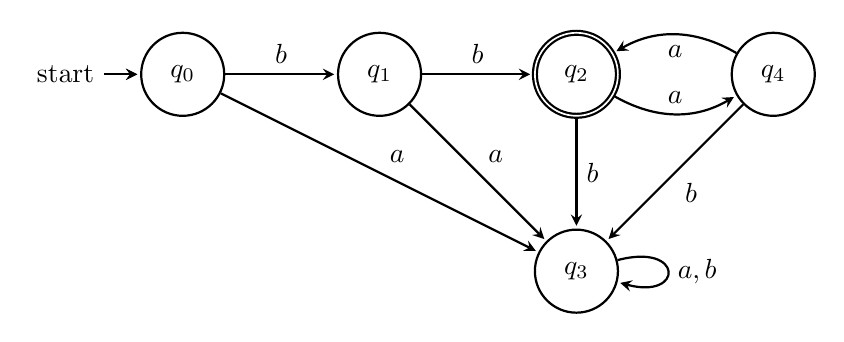
\begin{tikzpicture}[>=stealth, shorten >=1pt, node distance=2.5cm, on grid, auto, state/.append style={minimum size=3em}, thick ]
			\node[state, initial]				(A)               	{$q_0$};
			\node[state] 						(B) [right of=A] 	{$q_1$};
			\node[state, accepting]				(C) [right of=B] 	{$q_2$};
			\node[state]						(D) [below of=C] 	{$q_3$};
			\node[state]						(E)	[right of=C]	{$q_4$};
			\path[->] (A) +(-1,0) edge (A)
			
			%Transições:
			%(Partida) edge [tipo da seta] node {simbolo lido} (Destino)
			(A) edge			  				node {$b$}		 (B)
			(A) edge			  				node {$a$}		 (D)
			(B) edge			  				node {$b$}		 (C)
			(B) edge			  				node {$a$}		 (D)
			(C) edge			  				node {$b$}		 (D)
			(C) edge [bend right] 			  	node {$a$}		 (E)
			(E) edge [bend right] 			  	node {$a$}		 (C)
			(E) edge			  				node {$b$}		 (D)
			(D) edge [loop right] 			  	node {$a,b$}	 ( );
		\end{tikzpicture}
		\caption{AFD $A_1$ que reconhece a linguagem $\{bba^{2n} \mid n \in \mathbb{N}\}$.}
		\label{fig:AFDLinguagem1}
	\end{figure}
	
	\begin{proof}
		$(\Rightarrow)$ Suponha que $w \in L$ assim $w = bba^{2n}$ e por indução sobre o tamanho das palavras tem-se que,
		\begin{itemize}
			\item \textbf{Base da indução}:
			
			Quando $n = 0$ vale que $w = bba^{2\cdot 0}$ e usando a definição do AFD tem-se que, 
			$$\widehat{\delta}(q_0, bba^{2\cdot 0}) = \widehat{\delta}(q_0, bb) = \delta(\widehat{\delta}(q_0, b), b) = \delta(\delta(\widehat{\delta}(q_0, \lambda), b), b) = q_2$$
			como $q_2 \in F$ tem-se que $bb \in \mathcal{L}(A_1)$.
			
			\item \textbf{Hipótese indutiva (HI)}:
			
			Suponha que para todo $n \in \mathbb{N}$ tem-se que $\widehat{\delta}(q_0, bba^{2n}) \in F$, ou seja, $\widehat{\delta}(q_0, bba^{2n}) = q_2$.
			
			\item \textbf{Passo indutivo}:
			
			Dado $w = bba^{2(n+1)}$ tem-se que
			\begin{eqnarray*}
				\widehat{\delta}(q_0, bba^{2(n+1)}) & = & \widehat{\delta}(q_0, bba^{2n + 2})\\
				& = & \widehat{\delta}(q_0, bba^{2n}aa)\\
				& = & \delta(\delta(\widehat{\delta}(q_0, bba^{2n}), a), a)\\
				& \stackrel{\textbf{(HI)}}{=} & \delta(\delta(q_2, a), a)\\
				& = & \delta(q_3, a)\\
				& = & q_2
			\end{eqnarray*} 
			Logo $\widehat{\delta}(q_0, bba^{2n}) \in \mathcal{L}(A_1)$.
		\end{itemize} 
		$(\Leftarrow)$ Suponha que $w \in \mathcal{L}(A_1)$, assim pela definição do AFD $A_1$ tem-se que $\widehat{\delta}(q_0, w) = q_2$, entretanto, pela definição de $\delta$ (ver Figura \ref{fig:AFDLinguagem1}) tem-se que $q_2$ só é acessado pelas transições $\delta(q_1, b)$ e $\delta(q_4, a)$, ou seja, $w = w_1a$ ou $w = w_2b$ com $w_1, w_2 \in \Sigma^*$. Agora analisando cada possibilidade em separado tem-se que: 
		\begin{itemize}
			\item Para realizar o acesso via $q_1$ é necessário obviamente chegar em $q_1$ e isso só é possível a partir da transição $\delta(q_0, b)$, logo o acesso a $q_2$ via $q_1$ só é permitido para palavras com o prefixo $bb$, agora como toda palavra é prefixo de si mesmo isso já garante que $bb \in \mathcal{L}(A_1)$.
			\item Já o acesso via $q_4$ só é permitido pela transição $\delta(q_2, a)$ e como visto no caso anterior tem-se que o estado $q_2$ só pode ser acessado por palavras com prefixo $bb$, note porém, que as transições $\delta(q_2, a) = q_4$ e $\delta(q_4, a) = q_2$ formam um \textit{loop} e assim pode-se concluir que o acesso a $q_2$ via $q_4$ obrigatoriamente é realizado por palavras da forma $bba^{2n}$ com $n \geq 1$.
		\end{itemize}
		Note que a palavra $bb$ pode ser escrita como sendo $bba^0$, portanto, pelas duas análises anteriores pode-se concluir que se $\widehat{\delta}(q_0, w) = q_2$, então $w = bba^{2n}$ com $n \in \mathbb{N}$, e portanto, $w \in L$, completando assim a prova. 
	\end{proof}
\end{example}

\begin{example}
	O AFD $A$ do Exemplo \ref{exe:AFD} reconhece a linguagem $L = \{a^{2n + 1} \mid n \in \mathbb{N}\}$.
	\begin{proof}
		$(\Rightarrow)$ Suponha que $w \in L$ assim $w = a^{2n+1}$, agora por indução sobre o tamanho das palavras tem-se que, 
		
		\begin{itemize}
			\item \textbf{Base da indução}:
			
			Quando $n = 0$ vale a igualdade $w = a^{2\cdot 0+1}$, agora usando a definição do AFD $A$ tem-se que, 
			\begin{eqnarray*}
				\widehat{\delta}(q_0, a^{2\cdot 0+1}) = \widehat{\delta}(q_0, a^{1}) = \delta(\widehat{\delta}(q_0, \lambda), a) = \delta(q_0, a) = q_1
			\end{eqnarray*}
			e como $q_1 \in F$ tem-se que $a^{2\cdot 0+1} \in \mathcal{L}(A)$, ou seja, $w \in \mathcal{L}(A)$.
			
			\item \textbf{Hipótese indutiva (HI)}:
			
			Suponha que para todo $n \in \mathbb{N}$ tem-se que $\widehat{\delta}(q_0, a^{2n+1}) \in F$, ou seja, $\widehat{\delta}(q_0, a^{2n+1}) = q_1$.
			
			\item \textbf{Passo indutivo}:
			
			Dado $w = a^{2(n+1)+1}$ tem-se que,
			
			\begin{eqnarray*}
				\widehat{\delta}(q_0, a^{2(n+1)+1}) & = & \widehat{\delta}(q_0, a^{2n+1+2})\\
				& = & \widehat{\delta}(q_0, a^{2n+1}aa)\\
				& = & \delta(\delta(\widehat{\delta}(q_0, a^{2n+1}), a), a)\\
				& \stackrel{\textbf{(HI)}}{=} & \delta(\delta(q_1, a), a)\\
				& = & \delta(q_0, a)\\
				& = & q_1
			\end{eqnarray*}
		\end{itemize}
		$(\Leftarrow)$ A volta fica como exercício argumentativo ao leitor.
	\end{proof}
\end{example}

Pode-se agora formalizar a primeira das classes de linguagens sendo esta a classe das linguagens regulares, tal classe foi primeiramente definida por Kleene em seu trabalho \cite{kleene1951}, entretanto, em tal ocasião tais linguagens foram chamadas de eventos regulares, como será visto é momentos futuros nesse manuscrito a classe das linguagens regulares é aquela que possui o menor nível complexidade computacional.

\begin{definition}[Linguagens Regulares]\label{def:LinguagensRegulares}
	Uma linguagem $L$ qualquer é dita ser regular se, e somente se, existe um AFD $A$ tal que $L = \mathcal{L}(A)$. A classe de todas as linguagens regulares é denotada por $\mathcal{L}_{Reg}$.
\end{definition}


\section{Autômato Finito Não-determinístico}\label{sec:AFN}

Como explicado por Peter Linz em \cite{linz2006}, um autômato finito não-determinístico, ou simplesmente AFN, é um autômato que se diferencia dos AFD apenas no quesito da função de transição. A diferença consiste no fato de que, enquanto a imagem da função de transição em um AFD é sempre um estado, nos AFN a imagem da  função de transição é um subconjunto de estados, em um sentido moderno da teoria dos autômatos, um AFN seria uma máquina que algumas transições geraria uma superposição de estados \cite{valdi2020phd}. Formalmente um AFN é como se segue.

\begin{definition}[Autômato Finito Não-determinístico]\label{def:AFN}
	Um AFN é uma estrutura $A = \langle Q, \Sigma, \delta_N, q_0, F\rangle$ onde: $Q, \Sigma, q_0$ e $F$ são da mesma forma que na Definição \ref{def:AFD}, já $\delta_N : Q \times \Sigma \rightarrow \wp(Q)$ é uma função total (chamada função de transição não determinística).
\end{definition}

\begin{example}\label{exe:AFN1}
	A estrutura $A = \langle \{q_0, q_1, q_2\}, \{a, b\}, \delta_N, q_0, \{q_0, q_1\}  \rangle$ onde a função $\delta$ é descrita pela Tabela \ref{tab:DeltaAFN1} a seguir é um AFN.
	
	\begin{table}[h]
		\centering
		\begin{tabular}{c|cc}
			\backslashbox{$Q$}{$\Sigma$}	& $a$ & $b$\\ \hline
			$q_0$  & $\{q_1\}$ & $\{q_0\}$\\
			$q_1$  & $\{q_2\}$ & $\{q_0, q_2\}$\\
			$q_2$  & $\{q_2\}$ & $\{q_1\}$\\ \hline
		\end{tabular}
		\caption{Tabela de transição para a função $\delta_N$ do AFN no Exemplo \ref{exe:AFN1}.}
		\label{tab:DeltaAFN1}
	\end{table}
\end{example}

A representação visual de um AFN usando grafos de transição é construída exatamente da mesma forma que a representação de um AFD, a diferença é o fato de poder existir múltiplas arestas rotuladas por um símbolo $a \in \Sigma$ saindo de um vértice $q_i$ e chegando nos vértices $q_j \in X$ onde $X \subseteq Q$ e existe a transição $\delta_N(q_i, a) = X$.

\

\begin{example}
	O grafo de transição representado na Figura \ref{fig:AFN1} a seguir é uma representação para o AFN do Exemplo \ref{exe:AFN1}.
	
	\begin{figure}[h]
		\centering
		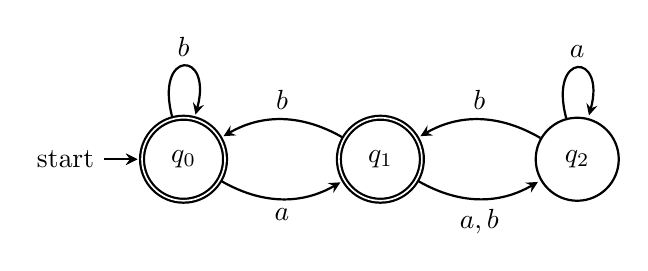
\begin{tikzpicture}[>=stealth, shorten >=1pt, node distance=2.5cm, on grid, auto, state/.append style={minimum size=3em}, thick ]
			\node[state, initial, accepting]	(A)               	{$q_0$};
			\node[state, accepting]				(B) [right of=A] 	{$q_1$};
			\node[state]				        (C) [right of=B] 	{$q_2$};
			\path[->] (A) +(-1,0) edge (A)
			
			%Transições:
			%(Partida) edge [tipo da seta] node {simbolo lido} (Destino)
			(A) edge [bend right]  				node [below] {$a$}		 (B)
			(A) edge [loop above]  				node 		 {$b$}		 ( )
			(B) edge [bend right]  				node [above] {$b$}		 (A)
			(B) edge [bend right]  				node [below] {$a, b$}	 (C)
			(C) edge [bend right] 				node [above] {$b$}		 (B)
			(C) edge [loop above]  				node {$a$}		 		 ( );
		\end{tikzpicture}
		\caption{Grafo de transição do AFN do Exemplo \ref{exe:AFN1}.}
		\label{fig:AFN1}
	\end{figure}
\end{example}

\begin{remark}
	Para as transições da forma $\delta_N(q_0, a) = \emptyset$ tem-se que as mesma não são representadas no grafo de transição de um AFN.
\end{remark}

Como para o caso determinístico a função de transição, neste caso $\delta_N$, pode ser estendida para uma função $\widehat{\delta_N}$ usando recursividade como se segue.

\begin{definition}[Transição não-determinística estendida]\label{def:FuncaoDeltaNDEstendida}
	Seja $A = \langle Q, \Sigma, \delta_N, q_0, F\rangle$ um AFN, a função de transição estendida é uma função $\delta_N: Q \times \Sigma^* \rightarrow \wp(Q)$ definida pela seguinte recursão.
	\begin{eqnarray}\label{eq:FuncaoDeltaNDEstendida}
		\widehat{\delta_N}(q, \lambda)& = & \{q\} \\
		\widehat{\delta_N}(q, wa)& = & \bigcup_{q' \in \widehat{\delta_N}(q, w)} \delta_N(q', a)
	\end{eqnarray}
\end{definition}


Como para os AFD a noção de computação em qualquer AFN consiste simplesmente da aplicação da função $\widehat{\delta_N}$ sobre alguma palavra $w \in \Sigma^*$ e um estado $q$. 

\begin{example}\label{exe:ComputacaoAFN}
	Considerando o AFN ilustrado na Figura \ref{fig:AFN1} e a palavra $``abb$'' tem-se que,
	\begin{eqnarray}\label{eq:AFNComptuacao1}
		\widehat{\delta_N}(q_0, abb) & = & \bigcup_{q' \in \widehat{\delta_N}(q_0, ab)} \delta_N(q', b)
	\end{eqnarray}
	mas tem-se que, 
	\begin{eqnarray}\label{eq:AFNComptuacao2}
		\widehat{\delta_N}(q_0, ab) & = & \bigcup_{q'' \in \widehat{\delta_N}(q_0, a)} \delta_N(q'', b)
	\end{eqnarray}
	e
	\begin{eqnarray}\label{eq:AFNComptuacao3}
		\widehat{\delta_N}(q_0, a) & = & \bigcup_{q''' \in \widehat{\delta_N}(q_0, \lambda)} \delta_N(q''', a) \nonumber \\ 
		& = & \bigcup_{q''' \in \{q_0\}} \delta_N(q''', a) \\
		& = & \delta_N(q_0, a) \nonumber \\ 
		& = & \{q_1\} \nonumber
	\end{eqnarray}
	substituindo a Equação (\ref{eq:AFNComptuacao3}) na Equação (\ref{eq:AFNComptuacao2}) tem-se que, 
	\begin{eqnarray}\label{eq:AFNComptuacao4}
		\widehat{\delta_N}(q_0, ab) & = & \{q_0, q_2\}
	\end{eqnarray}
	e finalmente substituindo a Equação (\ref{eq:AFNComptuacao4}) na Equação (\ref{eq:AFNComptuacao1}) tem-se que,
	\begin{eqnarray}
		\widehat{\delta_N}(q_0, aba) & = & \{q_0, q_1\}
	\end{eqnarray}
	ou seja, a computação da palavra $``abb$'' pelo AFN da Figura \ref{fig:AFN1} termina no conjunto de estados $\{q_0, q_1\}$.
\end{example}


Pelo exemplo anterior o leitor mais atento pode ter notado que diferente do caso determinístico, a computação em um AFN não é linear, no sentido de que não existe um único caminho de computação\footnote{Como explicado em \cite{valdi2020phd} um caminho de computação é uma sequência de estados assumidos pela unidade central do autômato durante o processamento de uma palavra de entrada.}, em vez disso, a computação em um AFN pode ser vista como uma árvore em que a união dos estados em cada nível da árvore representa a superposição de estados assumida pela unidade de controle do autômato a cada símbolo consumido (computado ou lido) da palavra $w$, o exemplo a seguir ilustra bem essa ideia de árvore de computação.

\begin{example}\label{exe:ArvoreComputacaoAFN}
	Considerando o AFN ilustrado na Figura \ref{fig:AFN1} e a palavra ``$abab$'' tem-se que o processo de computação para tal palavra poder ser representado pela árvore da Figura \ref{fig:ArvoreComputacaoAFN} a seguir.
	
	\begin{figure}[h]
		\centering
		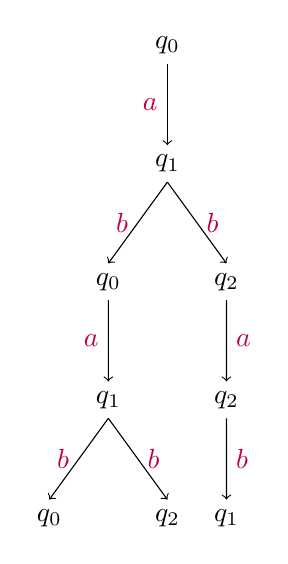
\begin{tikzpicture}
			\node {$q_0$}
			child { node {$q_1$} 
				child {node {$q_0$}
					child {node {$q_1$}
						child {node {$q_0$}
							edge from parent [->] node [left, purple] {$b$}
						}
						child {node {$q_2$}
							edge from parent [->] node [right, purple] {$b$}
						}
						edge from parent [->] node [left, purple] {$a$}
					}
					edge from parent [->] node [left, purple] {$b$}
				}
				child {node {$q_2$}
					child {node {$q_2$}
						child {node {$q_1$}
							edge from parent [->] node [right, purple] {$b$}
						}
						edge from parent [->] node [right, purple] {$a$}
					}
					edge from parent [->] node [right, purple] {$b$}
				}
				edge from parent [->] node [left, purple] {$a$}
			}
			;
		\end{tikzpicture}
		\caption{Árvore de computação da palavra ``$abab$'' no AFN da Figura \ref{fig:AFN1}.}
		\label{fig:ArvoreComputacaoAFN}
	\end{figure}
\end{example}

Pode-se agora apresentar a noção de aceitação (reconhecimento ou computação) de palavras nos AFD.

\begin{definition}[Reconhecimento de palavras em AFN]\label{defi:PalavraAceitaPorAFN}
	Sejam $A = \langle Q, \Sigma, \delta_N, q_0, F\rangle$ um AFN e seja $w \in \Sigma^*$. A palavra $w$ é dita aceita (reconhece ou computada) por $A$ sempre que $\widehat{\delta}(q_0, w) \cap F \neq \emptyset$ e é rejeitada por $A$ em qualquer outro caso.
\end{definition}

Note que a Definição \ref{defi:PalavraAceitaPorAFN} pode ser informalmente interpretada da seguinte forma, uma palavra é aceita por um AFN $A$ se existe pelo menos um caminho de computação para $w$ que termine em um estado final, isto é, pelo menos uma das folhas na árvore de computação deve ser um estado $q \in F$, neste caso $w$ é aceita por $A$.´

\begin{example}\label{exe:AceitacaoEmAFN}
	Considerando o AFN representado pela Figura \ref{fig:AFN2} a seguir,
	
	\begin{figure}[h]
		\centering
		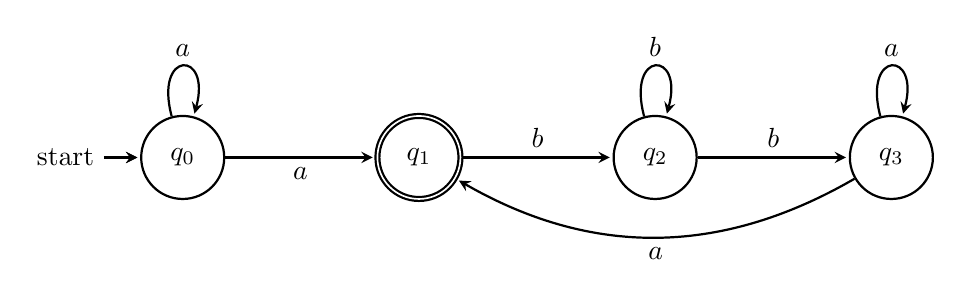
\begin{tikzpicture}[>=stealth, shorten >=1pt, node distance=3.0cm, on grid, auto, state/.append style={minimum size=3em}, thick ]
			\node[state, initial]				(A)               	{$q_0$};
			\node[state, accepting]				(B) [right of=A] 	{$q_1$};
			\node[state]				        (C) [right of=B] 	{$q_2$};
			\node[state]				        (D) [right of=C] 	{$q_3$};
			\path[->] (A) +(-1,0) edge (A)
			
			%Transições:
			%(Partida) edge [tipo da seta] node {simbolo lido} (Destino)
			(A) edge 			 				node [below] {$a$}		 (B)
			(A) edge [loop above]  				node 		 {$a$}		 ( )
			(B) edge 			  				node [above] {$b$}		 (C)
			(C) edge [loop above]  				node 		 {$b$}		 ( )
			(C) edge 			  				node [above] {$b$}		 (D)
			(D) edge [loop above]  				node 		 {$a$}		 ( )
			(D) edge [bend left]  				node [below] {$a$}		 (B);
		\end{tikzpicture}
		\caption{Grafo de transição de um AFN do Exemplo \ref{exe:AceitacaoEmAFN}.}
		\label{fig:AFN2}
	\end{figure}
	
	
	\noindent para as palavras ``$aabbbba$'' e ``$aabb$'' tem-se que: 
	$$\widehat{\delta_N}(q_0, aabbbba) = \{q_1, q_3\}$$ 
	e  
	$$\widehat{\delta_N}(q_0, aabb) = \{q_2, q_3\}$$ 
	logo a palavra ``$aabbbba$'' é aceita por tal AFN. Por outro lado, a palavra ``$aabb$'' não é aceita pelo AFN.
\end{example}

Usando a definição apresentada anteriormente de palavra aceita pode-se finalmente introduzir formalmente a noção de linguagem aceita (computada ou reconhecida) pelos AFN.

\begin{definition}[Linguagem de um AFN]\label{def:LinguagemAFN}
	Seja $A = \langle Q, \Sigma, \delta_N, q_0, F\rangle$ um AFN a linguagem reconhecida (ou computada) por $A$, denotada por $\mathcal{L}(A)$, corresponde ao conjunto de todas as palavras aceitas por $A$, formalmente tem-se que:
	\begin{eqnarray}
		\mathcal{L}(A) = \{w \in \Sigma^* \mid \widehat{\delta_N}(q_0, w) \cap F \neq \emptyset\}
	\end{eqnarray}
\end{definition}

De forma similar ao que ocorre com os AFD, para mostrar que uma linguagem $L$ é aceita por algum AFN $A$ deve-se provar a igualdade $L = \mathcal{L}(A)$, ou seja, deve-se provar que $w \in L \Longleftrightarrow w \in \mathcal{L}(A)$.

\begin{example}\label{exe:LinguagemAFN1}
	A linguagem $L = \{a^i(ba)^j \mid i \geq 1,j \geq 0\}$ é aceita pelo AFN $A$ representado pelo grafo de transição da Figura \ref{fig:AFN3} a seguir.
	
	\begin{figure}[h]
		\centering
		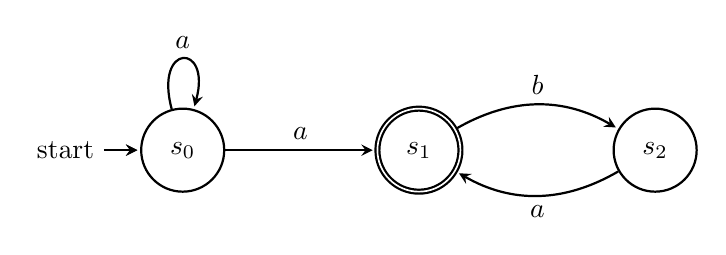
\begin{tikzpicture}[>=stealth, shorten >=1pt, node distance=3.0cm, on grid, auto, state/.append style={minimum size=3em}, thick ]
			\node[state, initial]				(A)               	{$s_0$};
			\node[state, accepting]				(B) [right of=A] 	{$s_1$};
			\node[state]				        (C) [right of=B] 	{$s_2$};
			\path[->] (A) +(-1,0) edge (A)
			
			%Transições:
			%(Partida) edge [tipo da seta] node {simbolo lido} (Destino)
			(A) edge [loop above]  				node 		 {$a$}		 ( )
			(A) edge 			  				node 		 {$a$}		 (B)
			(B) edge [bend left]  				node 		 {$b$}		 (C)
			(C) edge [bend left]  				node 		 {$a$}		 (B);
		\end{tikzpicture}
		\caption{Grafo de transição de um AFN.}
		\label{fig:AFN3}
	\end{figure}
	
	\begin{proof}
		$(\Rightarrow)$ Suponha que $w \in L$, portanto, $w = a^m(ba)^n$,  e agora por indução dupla sobre o par $(m,n)$ tem-se que:
		
		\begin{itemize}
			\item \textbf{Base da indução}:
			
			Quando com $m = 1$ e $n = 0$ vale a igualdade $w = a^1(ba)^0 = a$, agora usando a definição de $\delta_N$ do AFN $A$ como representado na Figura \ref{fig:AFN3} tem-se que, 
			\begin{eqnarray*}
				\widehat{\delta_N}(s_0, a) = \bigcup_{s' \in \widehat{\delta}(s_0, \lambda)} \delta_N(s', a) = \delta_N(s_0, a) = \{s_0, s_1\}
			\end{eqnarray*}
			uma vez que, $s_1 \in F$ tem-se que $\widehat{\delta_N}(s_0, a) \cap F \neq \emptyset$, e portanto, $w \in \mathcal{L}(A)$. Agora suponha que para $w = a^1(ba)^n$ com $n \geq 0$ tem-se que $\widehat{\delta_N}(s_0, a^1(ba)^n) \cap F \neq \emptyset$. Assim dado $a^1(ba)^{n+1}$ por definição tem-se que:
			\begin{eqnarray}\label{eq:ProvaAFNLinguagem1}
				\widehat{\delta_N}(s_0, a^1(ba)^{n+1}) & = & \widehat{\delta_N}(s_0, a^1(ba)^{n}ba)\nonumber\\
				& = & \bigcup_{s' \in \widehat{\delta_N}(s_0, a^1(ba)^{n}b)} \delta_N(s', a)
			\end{eqnarray}
			agora fazendo,
			\begin{eqnarray}\label{eq:ProvaAFNLinguagem2}
				K = \bigcup_{s'' \in \widehat{\delta_N}(s_0, a^1(ba)^{n})} \delta_N(s'', b)
			\end{eqnarray}
			e reescrevendo a Equação (\ref{eq:ProvaAFNLinguagem1}) usando a Equação (\ref{eq:ProvaAFNLinguagem2}) tem-se que,
			\begin{eqnarray}\label{eq:ProvaAFNLinguagem3}
				\widehat{\delta_N}(s_0, a^1(ba)^{n+1}) & = & \bigcup_{s' \in K} \delta_N(s', a)
			\end{eqnarray}
			entretanto, por hipótese tem-se que $\widehat{\delta_N}(s_0, a^1(ba)^n) \cap F \neq \emptyset$, consequentemente, tem-se que $s_1 \in \widehat{\delta_N}(s_0, a^1(ba)^n)$ dessa forma pela Equação (\ref{eq:ProvaAFNLinguagem2}) é claro que $\delta_N(s_1, b) \subseteq K$. Mas $\delta_N(s_1, b) = \{s_2\}$ logo pela Equação (\ref{eq:ProvaAFNLinguagem3}) tem-se que $\delta_N(s_2, a) \subseteq \widehat{\delta_N}(s_0, a^1(ba)^{n+1})$, desde que $\delta_N(s_2, a) = \{s_1\}$, tem-se $s_1 \in \widehat{\delta_N}(s_0, a^1(ba)^{n+1})$, portanto, $\widehat{\delta_N}(s_0, a^1(ba)^{n+1}) \cap F \neq \emptyset$, consequentemente $a^1(ba)^{n+1} \in \mathcal{L}(A)$.
			\item \textbf{Hipótese indutiva (HI)}:
			
			Assuma que para todo $n \geq 0$ tem-se que $\widehat{\delta_N}(s_0, a^m(ba)^n)  \cap F \neq \emptyset$.
			\item \textbf{Passo indutivo}:
			
			Primeiro seja $w \in L$ de forma que $w = a^{m+1}(ba)^0$ logo pela hipótese indutiva segue que, 
			\begin{eqnarray*}
				\widehat{\delta_N}(s_0, a^{m+1}(ba)^0) \cap F \neq \emptyset
			\end{eqnarray*}
			consequentemente, $a^{m+1}(ba)^0 \in \mathcal{L}(A)$. Por outro lado, sendo $w \in L$ tal que $w = a^{m+1}(ba)^n$, usando a  definição de $\widehat{\delta_N}$ tem-se para $a^{m+1}(ba)^{n+1}$ que, 
			\begin{eqnarray}\label{eq:ProvaAFNLinguagem4}
				\widehat{\delta_N}(s_0, a^{m+1}(ba)^{n+1}) & = & \widehat{\delta_N}(s_0, a^{m+1}(ba)^{n}ba)\nonumber\\
				& = & \bigcup_{s' \in \widehat{\delta_N}(s_0, a^{m+1}(ba)^{n}b)} \delta_N(s', a)
			\end{eqnarray}
			agora desenvolvendo o termo $\widehat{\delta_N}(s_0, a^{m+1}(ba)^{n}b)$ tem-se
			\begin{eqnarray*}
				\widehat{\delta_N}(s_0, a^{m+1}(ba)^{n}b) & = & \bigcup_{s'' \in \widehat{\delta_N}(s_0, a^{m+1}(ba)^{n})} \delta_N(s'', b)
			\end{eqnarray*}
			pela hipótese indutiva tem-se que $\widehat{\delta_N}(s_0, a^{m+1}(ba)^{n}) \cap F = \emptyset$, consequentemente, $s_1 \in \widehat{\delta_N}(s_0, a^{m+1}(ba)^{n})$, logo $\delta_N(s_1, b) \subseteq \widehat{\delta_N}(s_0, a^{m+1}(ba)^{n})$, uma vez que, $\delta_N(s_1, b) = \{s_2\}$, tem-se que $\{s_2\} \subseteq \widehat{\delta_N}(s_0, a^{m+1}(ba)^{n})$, assim pela Equação (\ref{eq:ProvaAFNLinguagem4}) segue que $\delta_N(s_2, a) \subseteq \widehat{\delta_N}(s_0, a^{m+1}(ba)^{n+1})$, mas por definição $\delta_N(s_2, a) = \{s_1\}$, portanto, tem-se que $\{s_1\} \subseteq \widehat{\delta_N}(s_0, a^{m+1}(ba)^{n+1})$, logo $\widehat{\delta_N}(s_0, a^{m+1}(ba)^{n+1}) \cap F \neq \emptyset$ e assim $a^{m+1}(ba)^{n+1} \in \mathcal{L}(A)$.
		\end{itemize}
		$(\Leftarrow)$ Suponha que $w \in \mathcal{L}(A)$ assim $s_1 \in \widehat{\delta_N}(s_0, w)$, note porém que $s_1$ só é acessível a partir de duas transições: 
		\begin{itemize}
			\item (1) $\delta_N(s_0, a)$ e
			\item (2) $\delta_N(s_2, a)$. 
		\end{itemize}
		Note que devido ao \textit{loop} fornecido pelo fato de que $s_0 \in \delta_N(s_0, a)$ a transição (1) pode ser executada $m$ vezes com $m \geq 1$, em que para cada execução um novo ramo com o estado $s_1$ é gerado na árvore de computação de $A$, entretanto, executar $m$ vezes a transição $\delta_N(s_0, a)$ implica em executar a computação $\widehat{\delta_N}(s_0, a^m)$, pelo fato\footnote{Fica para o leitor a tarefa de provar que para todo $m \geq 1$ tem-se que $s_1 \in \widehat{\delta_N}(s_0, a^m)$.} de que $s_1 \in \widehat{\delta_N}(s_0, a^m)$ tem-se que $a^m \in \mathcal{L}(A)$, e uma vez que $a^m = a^m(ba)^0$ tem-se que a primeira forma de $\widehat{\delta_N}(s_0, w) \cap F \neq \emptyset$ é que $w = a^m(ba)^0$ e assim $w \in L$. Por outro lado, para acessar $s_1$ via a transição (2) é necessário antes chegar a um ramo de computação em que o estado $s_2$ seja uma folha, mas pela definição de $A$ isso só é possível se a transição $\delta_N(s_1, b)$ for usada, note entretanto, que as transições $\delta_N(s_1, b) = \{s_2\}$ e $\widehat{\delta_N}(s_2, a) = \{s_1\}$ também geram um \textit{loop} que pode ser executado $n$ vezes com $n \geq 0$, mas executar esse \textit{loop} $n$ vezes corresponde a executar $\widehat{\delta_N}(s_1, (ba)^n)$, e como dito anteriormente, $s_1$ só é acessível pela definição de $A$ usando a computação $\widehat{\delta_N}(s_0, a^m)$, portanto, para que $s_1 \in \widehat{\delta_N}(s_0, w) \cap F$, obrigatoriamente, $w = a^m(ba)^n$ com $m \geq 1, n \geq 0$, e portanto, $w \in L$.
	\end{proof}
\end{example}

\begin{example}\label{exe:LinguagemAFN2}
	O AFN $S$ representado no grafo de transição exposto na Figura \ref{fig:AFN4} a seguir reconhece a linguagem $L = \{uv \mid u \in \{0,1\}^*,  v \in \{0,1\}\}$.
	
	\begin{proof}
		$(\Rightarrow)$ A ida fica a cargo do leitor. $(\Leftarrow)$ Suponha que $w \in \mathcal{L}(A)$ assim por definição $\widehat{\delta_N}(s_0, w) \cap \{s_1, s_2\} \neq \emptyset$, agora pela definição de $\delta_N$ é claro que toda árvore de computação de $A$ apresenta a propriedade de sempre conter um dos estados $s_1$ ou $s_2$, mas nunca os dois simultaneamente\footnote{A prova desta propriedade fica como exercício ao leitor.}, além disso, o fato de $s_0 \in \widehat{\delta_N}(s_0, a)$ para todo $a \in \{0,1\}$, garante que qualquer palavra não a vazia $u$ sobre o alfabeto $\{0,1\}$ pode ser gerada, por fim, no último passo de computação é claro que $s_1$ ou $s_2$ será uma folha da árvore, entretanto, $s_1$ só será tal folha no caso da palavra terminar em $0$ caso contrário a folha será $s_2$, e portanto, todo $w \in \mathcal{L}(A)$ tem a foma $uv$ com $u \in \{0, 1\}^*$ e $v \in \{0,1\}$, consequentemente $w \in L$.
	\end{proof}

	\begin{figure}[h]
		\centering
		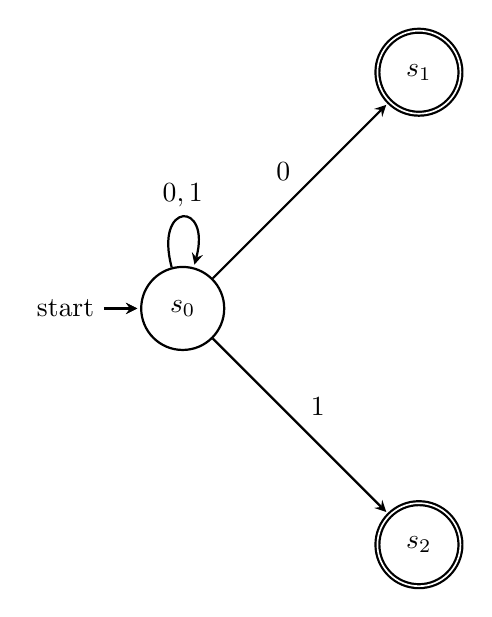
\begin{tikzpicture}[>=stealth, shorten >=1pt, node distance=3.0cm, on grid, auto, state/.append style={minimum size=3em}, thick ]
			\node[state, initial]						(A)               	{$s_0$};
			\node										(B) [right of=A] 	{ };
			\node[state, accepting]				        (C) [above of=B] 	{$s_1$};
			\node[state, accepting]				        (D) [below of=B] 	{$s_2$};
			\path[->] (A) +(-1,0) edge (A)
			
			%Transições:
			%(Partida) edge [tipo da seta] node {simbolo lido} (Destino)
			(A) edge [loop above]  				node 		 {$0, 1$}		 ( )
			(A) edge							node 		 {$0$}			 (C)
			(A) edge							node 		 {$1$}			 (D);
		\end{tikzpicture}
		\caption{Grafo de transição de um AFN $S$ do Exemplo \ref{exe:LinguagemAFN2}.}
		\label{fig:AFN4}
	\end{figure}
\end{example}

De forma ingênua o leitor pode vim a imaginar que a possibilidade da unidade de controle de um AFN poder assumir mais de um estado interno simultaneamente, faz com que os AFN sejam mais poderosos que os AFD, entretanto, como será exibido pelos resultados a seguir, isso não ocorre, de fato, como dito \cite{benjaLivro2010, linz2006} apesar de tornar mais fácil a tarefa de construir um autômato quem reconheça uma linguagem $L$, o não-determinismo não aumenta nem nada o poder de computação dos autômatos finitos.

\begin{theorem}[Transformação AFD - AFN]\label{teo:AFD-Para-AFN}
	Se $L = \mathcal{L}(A)$ para algum AFD $A$, então existe um AFN $A'$ tal que $L = \mathcal{L}(A')$.
\end{theorem}

\begin{proof}
	A prova é trivial, uma vez que, todo AFD $A = \langle Q, \Sigma, \delta, q_0, F\rangle$ pode ser convertido em um AFN $A' = \langle Q, \Sigma, \delta_N, q_0, F\rangle$ apenas realizando as transformações das transições $\delta(q_i, a) = q_j$ nas transições não-determinísticas $\delta_N(q_i, a) = \{q_j\}$ e mantendo todo o resto da estrutura igual.
\end{proof}

O próximo resultado estabelece a contraparte do Teorema \ref{teo:AFD-Para-AFN}, isto é, tal resultado mostrará que sempre é possível obter um AFD que pode ``simular''\footnote{O termo simular aqui, diz respeito a ideia de que cada aplicação de um função de transição não-determinística pode ser representada de forma precisa por uma aplicação de uma função de transição determinística, para detalhes consulte \cite{hopcroft2008, menezes1998LFA}.} um AFN.

\begin{theorem}[Transformação AFN - AFD]\label{teo:AFN-Para-AFD}
	Se $L = \mathcal{L}(A)$ para algum AFN $A$, então existe um AFD $A'$ tal que $L = \mathcal{L}(A')$.
\end{theorem}

\begin{proof}
	Suponha que $L = \mathcal{L}(A)$ para algum AFN $A = \langle Q, \Sigma, \delta_N, q_0, F\rangle$, agora é construído um  autômato $A' = \langle \wp(Q), \Sigma, \delta, \{q_0\}, F' \rangle$ onde para todo $X \in \wp(Q)$ e $a \in \Sigma$ tem-se
	\begin{eqnarray}\label{eq:TranformacaoDelta-DeltaN}
		\delta(X, a) = \bigcup_{q \in X} \delta_N(q, a)
	\end{eqnarray}
	claramente este autômato é realmente determinístico, e para todo $X \in \wp(Q)$  tem-se que $X \in F'$ se, e somente se, $X \cap F \neq \emptyset$. Agora será mostrado por indução sobre o tamanho de $w \in \Sigma^*$ que:
	$$\widehat{\delta}(\{q_0\}, w) = \widehat{\delta_N}(q_0, w)$$
	\begin{itemize}
		\item \textbf{Base da indução}:
		
		Quando $|w| = 0$ isto é $w = \lambda$ tem-se trivialmente pela definição das funções de transição estendidas que $\widehat{\delta}(\{q_0\}, \lambda) = \widehat{\delta_N}(q_0, \lambda)$.
		
		\item \textbf{Hipótese indutiva (HI)}:
		
		Suponha que para todo $w \in \Sigma^*$ com $|w| \geq 0$ tem-se que $\widehat{\delta}(\{q_0\}, w) = \widehat{\delta_N}(q_0, w)$.
		\item \textbf{Passo indutivo}:
		
		Dado $w = ua$ com $u \in \Sigma^*$, $|u| \geq 0$ e $a \in \Sigma$ tem-se que, 
		\begin{eqnarray*}
			\widehat{\delta}(\{q_0\}, w) & = & \widehat{\delta}(\{q_0\}, ua)\\
			& = & \delta(\widehat{\delta}(\{q_0\}, u), a)\\
			& \stackrel{\textbf{(HI)}}{=} & \delta(\widehat{\delta_N}(q_0, u), a)\\
			& \stackrel{Eq. (\ref{eq:TranformacaoDelta-DeltaN})}{=} & \bigcup_{q \in \widehat{\delta_N}(q_0, u)} \delta_N(q, a)\\
			& = & \widehat{\delta_N}(q_0, ua)\\
			& = & \widehat{\delta_N}(q_0, w)
		\end{eqnarray*}
	\end{itemize}
	Portanto, pode-se concluir que $w \in \mathcal{L}(A)$ se, e somente se, $w \in \mathcal{L}(A')$, ou seja, $L = \mathcal{L}(A')$ o que completa a prova.
\end{proof}

Observe que o método de construção usado na prova do Teorema \ref{teo:AFN-Para-AFD} cria um AFD cujo número de estado cresce em razão de uma potência de 2 quando comparado com o quantitativo de estados do AFN original. Como consequência deste resultado segue o seguinte corolário.

\begin{corollary}
	Uma linguagem $L$ é regular se, e somente se, existe um AFN $A$ tal que $L = \mathcal{L}(A)$.
\end{corollary}

\begin{proof}
	$(\Rightarrow)$ Assuma que $L$ é regular, assim por definição existe um AFD $A'$ tal que $L = \mathcal{L}(A')$, entretanto, pelo Teorema \ref{teo:AFD-Para-AFN} existe um AFN $A$ tal que $L = \mathcal{L}(A)$. $(\Leftarrow)$ Suponha que $L = \mathcal{L}(A)$ para algum AFN $A$, agora pelo Teorema \ref{teo:AFN-Para-AFD} existe um AFD $A'$ tal que $L = \mathcal{L}(A')$, e portanto, por definição $L$ é regular.
\end{proof}

É importante destacar que o método de construção do AFD usado na prova do Teorema \ref{teo:AFN-Para-AFD}, conhecido como método de construção das partes introduzido por Rabin e Scott em \cite{rabin1959}, tem a característica de poder vim a produzir durante sua execução alguns estados inacessíveis\footnote{Um estado $q$ em um AFD é dito inacessível se não existe um $w \in \Sigma^*$ tal que $\widehat{\delta}(q_0, w) = q$. Vale também ressaltar como destaco em \cite{benjaLivro2010, hopcroft2008} que estados inacessíveis não aumentam o poder de computação nos AFD.} no AFD resultante. 

Outro ponto sobre o método de construção das partes é que em alguns cenários pode ser tornar impraticável, pois se o AFN de entrada possuir $n$ estados, o AFD resultante do método terá $2^n$ estados, ou seja, o crescimento no número de estados do AFD resultante do método cresce proposicional a uma potência de 2, o que rapidamente gera um número exponencialmente grande de estados. 

A seguir o leitor será apresentado a uma melhoria no algoritmo de construção das partes, no sentido de que, a execução de tal algoritmo não produz estados inacessíveis no AFD de saída, o algoritmo a seguir é um pseudo-código baseado na versão textual apresentada no livro de Bedregal \textit{et al.} \cite{benjaLivro2010}. A melhoria no Algoritmo \ref{alg:AFN-AFD} consiste do fato dele não considerar simplesmente o conjunto $\wp(Q)$ no AFD de saída, em vez disso, ele constrói interativamente um conjunto de estados $Q' \subseteq \wp(Q)$, que no pior caso\footnote{A expressão ``no pior caso'' é típica da análise de algoritmos, em momentos futuros essa ideia de pior caso será melhor desenvolvida neste manuscrito.} $Q' = \wp(Q)$.

\begin{algorithm}[h]
	\Entrada{Um AFN $A = \langle Q, \Sigma, \delta_N, q_0, F\rangle$}
	\Saida{Um AFD $A' = \langle Q', \Sigma, \delta, \{q_0\}, F' \rangle$}
	\Inicio{
		Inicialize o conjuntos $Q_u$ com um  estado rotulado por $\{q_0\}$\\
		Inicialize o conjuntos $Q'$ com um  estado rotulado por $\{q_0\}$\\
		Inicialize o conjunto $F'$ como sendo vazio\\
		\Repita{$Q_u = \emptyset$}{
			Selecione um estado $X \in Q_u$\\
			\ParaCada{$a \in \Sigma$}{
				Determine o conjunto $\displaystyle Y = \bigcup_{q \in X}\delta_N(q, a)$\\
				\eSe{$Y \notin Q'$}{
					Adicione um estado rotulado por $Y$ em $Q'$\\
					Adicione um estado rotulado por $Y$ em $Q_u$\\
					Defina a transição $\delta(X, a) = Y$\\
				}{
					Defina a transição $\delta(X, a) = Y$\\
				}
			}
			Remova $X$ de $Q_u$
		}
		\ParaCada{$X \in Q'$}{
			\Se{$X \cap F \neq \emptyset$}{
				Adicione $X$ ao conjunto $F'$
			}
		}
		\Retorna{$A' = \langle Q', \Sigma, \delta, \{q_0\}, F' \rangle$}
	}
	\caption{Algoritmo para converter AFN em AFD sem estados inacessíveis.}
	\label{alg:AFN-AFD}
\end{algorithm}

\begin{example}\label{exe:ConvertendoAFN-AFD}
	Usando o Algoritmo \ref{alg:AFN-AFD}  tendo o AFN representado pelo grafo de transição da Figura \ref{fig:AFN2} como entrada será obtido o AFD $M = \langle \{s_0, s_1, s_2, s_3, s_4, \emptyset\}, \{a,b\}, \delta, s_0, F'\rangle$ onde tem-se os estados equivalem aos seguintes conjuntos $s_0 = \{q_0\}, s_1 = \{q_0, q_1\}, s_2 = \{q_2\},$ $s_3 = \{q_2, q_3\}, s_4 = \{q_1, q_3\}$ tem-se que $F' = \{s_1, s_4\}$ e a função de transição $\delta$ é como se segue. 
	\begin{eqnarray*}
		\delta(s_0, a) = s_1, \delta(s_1, a) = s_1, \delta(s_2, a) = \emptyset, \delta(s_3, a) = s_4, \delta(s_4, a) = s_4,  \delta(\emptyset, a) = \emptyset \\
		\delta(s_0, b) = \emptyset, \delta(s_1, b) = s_2, \delta(s_2, b) = s_3, \delta(s_3, b) = s_3, \delta(s_4, b) = s_2, \delta(\emptyset, b) = \emptyset
	\end{eqnarray*}
\end{example}

\section{$\lambda$-Autômatos Finitos Não-determinísticos}\label{sec:LAFN}

Os $\lambda$-Autômatos Finitos Não-determinísticos, ou simplesmente, $\lambda$-AFN são como dito em \cite{menezes1998LFA}, uma generalização do modelo de AFN que foi introduzido na seção anterior e que são permitidas transições entre estados diferentes usando (ou consumindo) a palavra vazia, tais transições recebem o nome de $\lambda$-transições, a seguir tais autômatos serão apresentados formalmente.

\begin{definition}[$\lambda$-Autômatos Finitos Não-determinísticos]\label{def:LAFN}
	Um $\lambda$-AFN é uma estrutura $A = \langle Q, \Sigma, \underline{\delta_N}, q_0, F\rangle$ onde: $Q, \Sigma, q_0$ e $F$ são da mesma forma que na Definição \ref{def:AFD}, já $\underline{\delta_N} : Q \times (\Sigma \cup \{\lambda\}) \rightarrow \wp(Q)$ é uma função total (chamada $\lambda$-função de transição não determinística).
\end{definition}

A representação usando grafos de transição dos $\lambda$-AFN e similar a representação dos AFN da seção anterior, a única diferença é que podem haver transições rotuladas pelo símbolo $\lambda$, isto é, podem existir no grafo arestas entre vértices que são rotuladas por $\lambda$, e o mesmo vale para a representação das árvores de computação.

\begin{example}\label{exe:LAFN1}
	A estrutura $A = \langle \{q_0, q_1, q_2\}, \{0,1\}, \underline{\delta_N}, q_0, \{q_0\}\rangle$ com $\underline{\delta_N}$ sendo especificada pela Tabela \ref{tab:DeltaLAFN1} a seguir é um $\lambda$-AFN.
	
	\begin{table}[h]
		\centering
		\scriptsize
		\begin{tabular}{c|ccc}
			\backslashbox{$Q$}{$\Sigma \cup \{\lambda\}$}	& $0$ & $1$ & $\lambda$\\ \hline
			$q_0$  & $\emptyset$ & $\emptyset$ & $\{q_1\}$\\
			$q_1$  & $\{q_1\}$ & $\{q_2\}$ & $\{q_2\}$\\
			$q_2$  & $\{q_2\}$ & $\{q_2\}$ & $\{q_0, q_2\}$ \\ \hline
		\end{tabular}
		\caption{Tabela de transição para a função $\delta_N$ do AFN no Exemplo \ref{exe:LAFN1}.}
		\label{tab:DeltaLAFN1}
	\end{table}
\end{example} 

\begin{remark}
	Uma interpretação para as transições da forma $\underline{\delta_N}(q, \lambda) = X$ é que a unidade de controle do autômato consegue mudar seu estado interno $q$ para um subconjunto de estados $X$ sem precisar acessar a memória.
\end{remark}

\begin{example}
	O grafo de transição representado na Figura \ref{fig:LAFN1} a seguir é uma representação para o $\lambda$-AFN do Exemplo \ref{exe:LAFN1}.
	
	\begin{figure}[h]
		\centering
		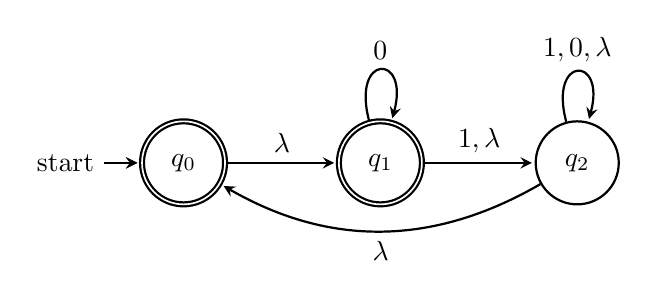
\begin{tikzpicture}[>=stealth, shorten >=1pt, node distance=2.5cm, on grid, auto, state/.append style={minimum size=3em}, thick ]
			\node[state, initial, accepting]	(A)               	{$q_0$};
			\node[state, accepting]				(B) [right of=A] 	{$q_1$};
			\node[state]				        (C) [right of=B] 	{$q_2$};
			\path[->] (A) +(-1,0) edge (A)
			
			%Transições:
			%(Partida) edge [tipo da seta] node {simbolo lido} (Destino)
			(A) edge							node 		 {$\lambda$} (B)
			(B) edge							node [above] {$1, \lambda$} (C)
			(B) edge [loop above]  				node 		 {$0$} 		 ( )
			(C) edge [loop above]  				node 		 {$1, 0, \lambda$} ( )
			(C) edge [bend left]  				node [below] {$\lambda$} (A);
		\end{tikzpicture}
		\caption{Grafo de transição do $\lambda$-AFN do Exemplo \ref{exe:LAFN1}.}
		\label{fig:LAFN1}
	\end{figure}
\end{example}

Note porém que a definição da função de transição $\underline{\delta_N}$ garante que as transições em um $\lambda$-AFN acontecem apenas em duas situações, a primeira em relação símbolos individuais do alfabeto $\Sigma$ e a segunda com relação a palavra vazia, assim não existe uma forma de computar uma palavra $w$ de forma que $|w| > 1$. A saída para contorna esse fato é estender a função de transição do autômato, similarmente ao que é feito para os AFD e AFN, para isso entretanto, é necessária algumas definições adicionais.

\begin{definition}[Função $\delta_\lambda$]\label{def:L-fecho}
	Seja $A = \langle Q, \Sigma, \underline{\delta_N}, q_0, F\rangle$ um $\lambda$-AFN, então a função $\delta_\lambda: Q \rightarrow \wp(Q)$ é definida como,
	\begin{equation}
		\delta_\lambda(q) = \bigcup_{i = 0}^n\lambda\text{-fecho}^i(q)
	\end{equation}
	onde $n = \# Q - 1$ e
	\begin{eqnarray}
		\lambda\text{-fecho}^0(q) & = & \{q\}\\
		\lambda\text{-fecho}^{i}(q) & = & \bigcup_{q' \in \lambda\text{-fecho}^{i-1}(q)} \delta_N(q', \lambda)
	\end{eqnarray}
\end{definition}

\begin{example}
	Considere o $\lambda$-AFN da Figura \ref{fig:LAFN1} tem-se para o estado $q_1$ que,
	\begin{eqnarray}\label{eq:LAFNeq1}
		\lambda\text{-fecho}^{2}(q_1) & = &  \bigcup_{q' \in \lambda\text{-fecho}^{1}(q_1)} \delta_N(q', \lambda)
	\end{eqnarray}
	desenvolvendo $q' \in \lambda\text{-fecho}^{1}(q_0)$ tem-se que,
	\begin{eqnarray*}
		\lambda\text{-fecho}^{1}(q_1) & = &  \bigcup_{q' \in \lambda\text{-fecho}^{0}(q_1)} \delta_N(q', \lambda)
	\end{eqnarray*}
	mas, 
	\begin{eqnarray*}
		\lambda\text{-fecho}^{0}(q_1) & = & \{q_1\}
	\end{eqnarray*}
	assim, 
	\begin{eqnarray*}
		\lambda\text{-fecho}^{1}(q_1) & = &  \{q_2\}
	\end{eqnarray*}
	substituindo tal resultado na Equação \ref{eq:LAFNeq1} tem-se que, 
	\begin{eqnarray*}\label{eq:LAFNeq2}
		\lambda\text{-fecho}^{2}(q_1) & = & \bigcup_{q' \in \{q_2\}} \delta_N(q', \lambda)\\
		& = & \{q_2, q_0\}
	\end{eqnarray*}
	logo $\delta_\lambda(q_1) = \{q_0, q_1, q_2\}$.
\end{example}

Uma interpretação semântica para a função $\delta_\lambda$ é que ela representa a resposta ao questionamento: ``Estando no estado $q$ e executando $n$ $\lambda$-transições qual subconjunto de estados a unidade central do autômato irá assumir?''. Assim como acontecer com as funções de transição a função $\delta_\lambda$ pode ser estendida, a seguir é exposto tal extensão.

\begin{definition}[Função $\widehat{\delta_\lambda}$]\label{def:L-Fecho}
	Seja $A = \langle Q, \Sigma, \underline{\delta_N}, q_0, F\rangle$ um $\lambda$-AFN, então a função $\widehat{\delta_\lambda}: \wp(Q) \rightarrow \wp(Q)$ é definida como,
	\begin{equation}
		\widehat{\delta_\lambda}(X) = \bigcup_{q \in X} \delta_\lambda(q)
	\end{equation}
\end{definition} 

\begin{example}
	Considere o $\lambda$-AFN da Figura \ref{fig:LAFN1} tem-se para o conjunto $\{q_1, q_2\}$ que,
	\begin{eqnarray*}
		\widehat{\delta_\lambda}(\{q_1, q_2\}) & = & \bigcup_{q \in \{q_1, q_2\}} \delta_\lambda(q)\\
		& = & \delta_\lambda(q_1) \cup \delta_\lambda(q_2)\\
		& = & \{q_0, q_1, q_2\} \cup \{q_0, q_2, q_1\}\\
		& = & \{q_0, q_2, q_1\}
	\end{eqnarray*}
\end{example}

Agora usando as definições de $\delta_\lambda$ e $\widehat{\delta_\lambda}$ pode-se apresentar a extensão da função de transição dos $\lambda$-AFN.

\begin{definition}[$\lambda$-Transição não-determinística estendida]\label{def:FuncaoLDeltaNDEstendida}
	Seja $A = \langle Q, \Sigma, \underline{\delta_N}, q_0, F\rangle$  um $\lambda$-AFN a função $\underline{\delta_N}$ é estendido para a função $\widehat{\underline{\delta_N}}: Q \times \Sigma^* \rightarrow \wp(Q)$ definida pela seguinte recursão:
	\begin{eqnarray}\label{eq:FuncaoLDeltaNDEstendida}
		\widehat{\underline{\delta_N}}(q, \lambda)& = &  \delta_\lambda(q)\\
		\widehat{\underline{\delta_N}}(q, wa) & = & \bigcup_{q' \in \widehat{\underline{\delta_N}}(q, w)} \widehat{\delta_\lambda}(\underline{\delta_N}(q', a))
	\end{eqnarray}
\end{definition}

\begin{example}
	Considere o $\lambda$-AFN da Figura \ref{fig:LAFN1} tem-se a seguinte computação para a palavra $``10''$:
	\begin{eqnarray}\label{eq:ExemLAFN1}
		\widehat{\underline{\delta_N}}(q_0, 10) & = & \bigcup_{q' \in \widehat{\underline{\delta_N}}(q_0, 1)} \widehat{\delta_\lambda}(\underline{\delta_N}(q', 0))\nonumber\\
		& = & \bigcup_{q' \in \widehat{\underline{\delta_N}}(q_0, 1)} \widehat{\delta_\lambda}(\underline{\delta_N}(q', 0))
	\end{eqnarray}
	mas,
	\begin{eqnarray}\label{eq:ExemLAFN2}
		\widehat{\underline{\delta_N}}(q_0, 1) & = & \bigcup_{q' \in \widehat{\underline{\delta_N}}(q_0, \lambda)} \widehat{\delta_\lambda}(\underline{\delta_N}(q', 1))\nonumber\\
		& = & \bigcup_{q' \in \delta_\lambda(q_0)} \widehat{\delta_\lambda}(\underline{\delta_N}(q', 1))\nonumber\\
		& = & \bigcup_{q' \in \{q_0, q_1, q_2\}} \widehat{\delta_\lambda}(\underline{\delta_N}(q', 1))\\
		& = & \widehat{\delta_\lambda}(\{q_1, q_2\})\nonumber\\
		& = & \{q_0, q_1, q_2\}\nonumber
	\end{eqnarray}
	substituindo o valor da Equação (\ref{eq:ExemLAFN2}) na Equação (\ref{eq:ExemLAFN1}) tem-se que, 
	\begin{eqnarray*}
		\widehat{\underline{\delta_N}}(q_0, 10) & = & \bigcup_{q' \in \{q_0, q_1, q_2\}} \widehat{\delta_\lambda}(\underline{\delta_N}(q', 0))\\
		& = & \{q_0, q_1, q_2\}
	\end{eqnarray*}
\end{example}

Assim como para o caso dos AFN uma palavra qualquer $w \in \Sigma^*$ será dita aceita por um $\lambda$-AFN quando a computação da palavra $w$ para em pelo menos um estado final, ou seja, $w$ é reconhecida pelo $\lambda$-AFN sempre que $\widehat{\underline{\delta_N}}(q_0, w) \cap F \neq \emptyset$, e assim pode-se definir formalmente a noção de linguagem para os $\lambda$-AFN.

\begin{definition}[Linguagem de um $\lambda$-AFN]\label{def:LinguagelLAFN}
	Seja $A = \langle Q, \Sigma, \underline{\delta_N}, q_0, F\rangle$ um $\lambda$-AFN a linguagem aceita por $A$, denotado por $\mathcal{L}(A)$, corresponde ao seguinte conjunto.
	\begin{eqnarray}
		\mathcal{L}(A) = \{w \in \Sigma^* \mid \widehat{\underline{\delta_N}}(q_0, w) \cap F \neq \emptyset\}
	\end{eqnarray}
\end{definition}

Os aspectos relacionados a mostrar que um $\lambda$-AFN reconhece uma linguagem $L$ são similares ao mesmo aspectos com respeito aos AFN.

\begin{example}\label{exe:LinguagemLAFN1}
	O $\lambda$-AFN representado pelo grafo de transição da Figura \ref{fig:Linguagem-LAFN1} a seguir reconhece a linguagem $L = \{w \in \{1,2,3\}^* \mid w = 1^i2^j3^k \text{ com } i,j,k \in \mathbb{N}\}$.
	
	\begin{figure}[h]
		\centering
		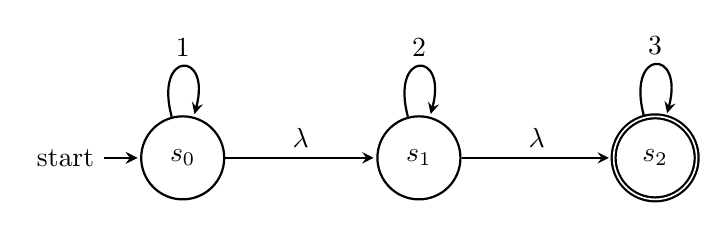
\begin{tikzpicture}[>=stealth, shorten >=1pt, node distance=3.0cm, on grid, auto, state/.append style={minimum size=3em}, thick ]
			\node[state, initial]						(A)               	{$s_0$};
			\node[state]								(B) [right of=A] 	{$s_1$};
			\node[state, accepting]				        (C) [right of=B] 	{$s_2$};
			\path[->] (A) +(-1,0) edge (A)
			
			%Transições:
			%(Partida) edge [tipo da seta] node {simbolo lido} (Destino)
			(A) edge [loop above]  				node 		 {$1$} 		 ( )
			(A) edge 			  				node 		 {$\lambda$} (B)
			(B) edge [loop above]  				node 		 {$2$} 		 ( )
			(B) edge 			  				node 		 {$\lambda$} (C)
			(C) edge [loop above]  				node 		 {$3$} 		 ( );
		\end{tikzpicture}
		\caption{Grafo de transição do $\lambda$-AFN do Exemplo \ref{exe:LinguagemLAFN1}.}
		\label{fig:Linguagem-LAFN1}
	\end{figure}
\end{example}

\begin{example}\label{exe:LinguagemLAFN2}
	O $\lambda$-AFN representado pelo grafo de transição esboçado pela Figura \ref{fig:Linguagem-LAFN2}, aceita a linguagem $L = \{uv \mid u \in \{a\}^*, |u|_a = 2k\text{ ou } |u|_a = 3k, v=bx, x \in \{a,b\}^*, k \in \mathbb{N}\}$.
\end{example}

\begin{figure}[h]
	\centering
	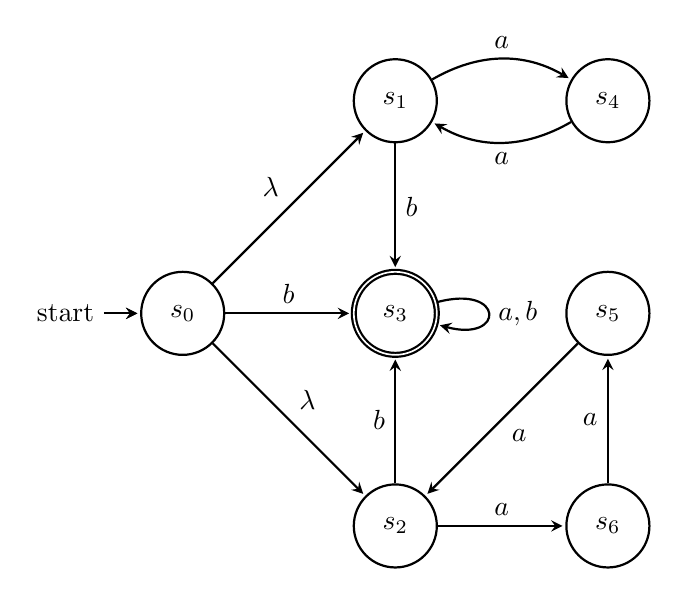
\begin{tikzpicture}[>=stealth, shorten >=1pt, node distance=2.7cm, on grid, auto, state/.append style={minimum size=3em}, thick ]
		\node[state, initial]				(A)               	{$s_0$};
		\node[state, accepting]				(B) [right of=A]	{$s_3$};
		\node[state] 						(C) [above of=B] 	{$s_1$};
		\node[state] 						(D) [below of=B] 	{$s_2$};
		\node[state]						(E) [right of=B] 	{$s_5$};
		\node[state] 						(F) [above of=E] 	{$s_4$};
		\node[state] 						(G) [right of=D] 	{$s_6$};
		
		
		\path[->] (A) +(-1,0) edge (A)
		
		%Transições:
		%(Partida) edge [tipo da seta] node {simbolo lido} (Destino)  [loop right]  
		(A) edge  							node 		 {$\lambda$}	 (C)
		(A) edge  							node 		 {$\lambda$}	 (D)
		(A) edge  							node 		 {$b$}	 		 (B)
		(B) edge [loop right]  				node 		 {$a,b$}		 ( )
		(C) edge [bend left]				node 		 {$a$}			 (F)
		(C) edge							node		 {$b$}			 (B)
		(F) edge [bend left]				node 		 {$a$}			 (C)
		(D) edge							node		 {$a$}			 (G)
		(G) edge							node		 {$a$}			 (E)
		(E) edge							node		 {$a$}			 (D)
		(D) edge							node		 {$b$}			 (B);
	\end{tikzpicture}
	\caption{Grafo de transição do $\lambda$-AFN do Exemplo \ref{exe:LinguagemLAFN2}.}
	\label{fig:Linguagem-LAFN2}
\end{figure}

\

\begin{theorem}[Transformação $\lambda$-AFN-AFD]\label{teo:LAFN-AFD}
	Se $L = \mathcal{L}(A)$ para algum $\lambda$-AFN $A$, então existe um  AFD $A'$ tal que $L = \mathcal{L}(A')$.
\end{theorem}

\begin{proof}
	Suponha que $L = \mathcal{L}(A)$ para algum $\lambda$-AFN $A =  \langle Q, \Sigma, \underline{\delta_N}, q_0, F \rangle$ agora defina o seguinte o autômato $A' = \langle \wp(Q), \Sigma, \delta, \delta_\lambda(q_0), F' \rangle$ onde para todo $X \in \wp(Q)$ tem-se que $X \in F'$ se, e somente se, $X \cap F \neq \emptyset$, e além disso, para todo $X \in \wp(Q)$ e $a \in \Sigma$ tem-se:
	\begin{eqnarray}\label{eq:LAFN-AFD}
		\delta(X, a) & = & \bigcup_{q \in X} \widehat{\delta_\lambda}\Big(\underline{\delta_N}(q, a)\Big)
	\end{eqnarray}
	por essa construção obviamente esse autômato é um AFD\footnote{A prova desse fato fica como exercício ao leitor.}. Agora será mostrado por indução sobre o tamanho de $w \in \Sigma^*$ que:
	$$\widehat{\delta}(\delta_\lambda(q_0), w) = \widehat{\underline{\delta_N}}(q_0, w)$$
	\begin{itemize}
		\item \textbf{Base da indução}:
		
		Quando $|w| = 0$ isto é $w = \lambda$ tem-se trivialmente pela definição das funções de transição estendidas que, 
		\begin{eqnarray*}
			\widehat{\delta}(\delta_\lambda(q_0), \lambda) & = & \delta_\lambda(q_0)\\
			& = & \widehat{\underline{\delta_N}}(q_0, \lambda)
		\end{eqnarray*}
		
		\item \textbf{Hipótese indutiva (HI)}:
		
		Suponha que para todo $w \in \Sigma^*$ com $|w| \geq 0$ tem-se que $\widehat{\delta}(\delta_\lambda(q_0), w) = \widehat{\underline{\delta_N}}(q_0, w)$.
		\item \textbf{Passo indutivo}:
		
		Dado $w = ua$ com $u \in \Sigma^*$, $|u| \geq 0$ e $a \in \Sigma$ tem-se que, 
		\begin{eqnarray*}
			\widehat{\delta}(\delta_\lambda(q_0), w) & = & \widehat{\delta}(\delta_\lambda(q_0), ua)\\
			& = & \delta(\widehat{\delta}(\delta_\lambda(q_0), u), a)\\
			& \stackrel{\textbf{(HI)}}{=} & \delta(\widehat{\underline{\delta_N}}(q_0, w), a)\\
			& \stackrel{Eq. (\ref{eq:LAFN-AFD})}{=} & \bigcup_{q \in \widehat{\underline{\delta_N}}(q_0, w)} \widehat{\delta_\lambda}\Big(\underline{\delta_N}(q, a)\Big)\\
			& = & \widehat{\underline{\delta_N}}(q_0, ua)\\
			& = & \widehat{\underline{\delta_N}}(q_0, w)
		\end{eqnarray*}
	\end{itemize}
	Portanto, pode-se concluir que $w \in \mathcal{L}(A)$ se, e somente se, $w \in \mathcal{L}(A')$, ou seja, $L = \mathcal{L}(A')$ o que completa a prova.
\end{proof}

\begin{theorem}[Transformação AFD-$\lambda$-AFN]\label{teo:AFD-LAFN}
	Se $L = \mathcal{L}(A)$ para algum AFD $A$, então existe um $\lambda$-AFN $A'$ tal que $L = \mathcal{L}(A')$.
\end{theorem}

\begin{proof}
	Trivial e ficará como exercício ao leitor.
\end{proof}

\begin{corollary}\label{col:RegularLAFN}
	Uma linguagem $L$ é regular se, e somente se, existe um $\lambda$-AFN $A$ tal que $L = \mathcal{L}(A)$.
\end{corollary}

\begin{proof}
	$(\Rightarrow)$ Assuma que $L$ é regular, assim por definição existe um AFD $A'$ tal que $L = \mathcal{L}(A')$, entretanto, pelo Teorema \ref{teo:AFD-LAFN} existe um $\lambda$-AFN $A$ tal que $L = \mathcal{L}(A)$. $(\Leftarrow)$ Suponha que $L = \mathcal{L}(A)$ para algum $\lambda$-AFN $A$, agora pelo Teorema \ref{teo:LAFN-AFD} existe um AFD $A'$ tal que $L = \mathcal{L}(A')$, e portanto, $L$ é regular.
\end{proof}

\begin{remark}
	Note que o Corolário \ref{col:RegularLAFN} estabelece que a existência de $\lambda$-transições não aumenta o poder de computação dos autômatos finitos.
\end{remark}

Assim como para o caso da transformação de AFN em AFD, o processo de usar a construção do conjunto das partes no Teorema \ref{teo:LAFN-AFD} possui a desvantagem de gera estados inacessíveis. Mas como discutido em \cite{benja-2011, benja-2015, hopcroft2008, linz2006}, algumas simples modificações no Algoritmo \ref{alg:AFN-AFD} fazem com que o novo algoritmo gerado seja capaz de remover as $\lambda$-transições e não sejam produzidos estados inacessíveis a seguir é apresentado este novo algoritmo.

\begin{example}
	Aplicando o Algoritmo \ref{alg:LAFN-AFD} ao $\lambda$-AFN do Exemplo \ref{exe:LinguagemLAFN2} é obtido como saída o AFD $D = \langle \{A_0, A_1, A_2, A_3, A_4, A_5, A_6, A_7, \emptyset\}, \{a,b\}, \delta, \{s_0, s_1, s_2\}, F' \rangle$ onde tem-se $A_0 = \{s_0, s_1, s_2\}, A_1 = \{s_4, s_6\}, A_2 = \{s_3\},$ $A_3 = \{s_1, s_5\}, A_4 = \{s_2, s_4\}, A_5 = \{s_1, s_6\},$ $A_6 = \{s_4, s_5\}$ e $A_7 = \{s_1, s_2\}$ com $F' = \{A_2\}$ e $\delta$ é descrito a seguir. 
	
	\begin{eqnarray*}
		\delta(A_0, a) = A_1, \delta(A_0, b) = A_2, \delta(A_1, a) = A_3,\\
		\delta(A_1, b) = \emptyset, \delta(A_2, a) = A_2, \delta(A_2, b) = A_2,\\
		\delta(A_3, a) = A_4, \delta(A_3, b) = A_2, \delta(A_4, a) = A_5, \\
		\delta(A_4, b) = A_2, \delta(A_5, a) = A_6, \delta(A_5, b) = A_2,\\
		\delta(A_6, a) = A_7, \delta(A_6, b) = \emptyset, \delta(A_7, a) = A_1,\\ 
		\delta(A_7, b) = A_2, \delta(\emptyset, a) = A_7, \delta(\emptyset, b) = \emptyset
	\end{eqnarray*}
\end{example}

\begin{remark}
	Argumentações sobre a corretude e a completude do Algoritmo \ref{alg:LAFN-AFD} podem ser consultadas em \cite{hopcroft2008}.
\end{remark}

\newpage

\begin{algorithm}[h]
	\Entrada{Um $\lambda$-AFN $A = \langle Q, \Sigma, \underline{\delta_N}, q_0, F\rangle$}
	\Saida{Um AFD $A' = \langle Q', \Sigma, \delta, \delta_\lambda(q_0), F' \rangle$}
	\Inicio{
		Inicialize o conjuntos $Q_u$ com um  estado rotulado por $\delta_\lambda(q_0)$\\
		Inicialize o conjuntos $Q'$ com um  estado rotulado por $\delta_\lambda(q_0)$\\
		Inicialize o conjunto $F'$ como sendo vazio\\
		\Repita{$Q_u = \emptyset$}{
			Selecione um estado $X \in Q_u$\\
			\ParaCada{$a \in \Sigma$}{
				Determine o conjunto $\displaystyle Y = \widehat{\delta_\lambda}\Big(\bigcup_{q \in X} \underline{\delta_N}(q, a)\Big)$\\
				\eSe{$Y \notin Q'$}{
					Adicione um estado rotulado por $Y$ em $Q'$\\
					Adicione um estado rotulado por $Y$ em $Q_u$\\
					Defina a transição $\delta(X, a) = Y$\\
				}{
					Defina a transição $\delta(X, a) = Y$\\
				}
			}
			Remova $X$ de $Q_u$
		}
		\ParaCada{$X \in Q'$}{
			\Se{$X \cap F \neq \emptyset$}{
				Adicione $X$ ao conjunto $F'$
			}
		}
		\Retorna{$A' = \langle Q', \Sigma, \delta, \delta_\lambda(q_0), F' \rangle$}
	}
	\caption{Algoritmo para remoção de $\lambda$-transições de um $\lambda$-AFN.}
	\label{alg:LAFN-AFD}
\end{algorithm}

\

\begin{note}
	Nestas últimas seções foram usados os símbolos $\delta, \delta_N$ e $\underline{\delta_N}$ para denotar as funções de transições dos AFD, AFN e $\lambda$-AFN respectivamente, entretanto, isso foi feito apenas para tornar o texto mais didático e ajudar na conversão entre os tipos de autômatos, mas é comum encontrar na literatura (ver \cite{benjaLivro2010, hopcroft2008, linz2006}) que independente do tipo de autômato sua função de transição é denotada apenas por $\delta$.
\end{note}

\section{Teorema Myhill-Nerode e a Minimização de AFD}\label{sec:Minimizacao}

Até agora este manuscrito se preocupou com a tarefa de saber se uma linguagem pode ou não ser reconhecida por um autômato finito,  seja ele determinístico ou não-determinístico. Nesta seção será apresentada ao leitor a questão de eficiência no reconhecimento de linguagens em relação aos autômatos finitos, aqui será mostrado que o problema de encontrar um menor AFD que reconhece uma linguagem $L$ é decidível. 

Na teoria dos autômatos quando se usa a palavra ``menor'', se está querendo dizer simplesmente aquele com o menor número possível de estados, ou seja, o AFD mínimo.  Mais adiante será aqui provado, que esse AFD mínimo é único a menos de isomorfismo, ou seja, se dois AFD reconhecem a mesma linguagem, cada um tendo o menor número possível de estados, então eles são são isomórficos. Isso significa que cada linguagem regular está associada com um AFD mínimo. 

Este resultado da existência de um AFD mínimo recebe o nome de \textbf{Teorema Myhill-Nerode}, em homenagem aos matemáticos John Myhill\footnote{O professor Myhill também é conhecido por seu Teorema de isomorfismo\cite{myhill1957-isomorfismo}, que pode ser visto como um análogo dentro da teoria da computabilidade ao teorema de Cantor–Bernstein–Schroeder e pelo famoso pelo Teorema  de Rice–Myhill–Shapiro, mais comumente conhecido como Teorema de Rice \cite{benjaLivro2010, rice1953-teorema-Rice}.} (1923-1987) e Anil Nerode (1932-), que o provaram na Universidade de Chicago em 1958 no artigo \cite{nerode1958}, de forma geral tal resultado fornece as condições suficientes e necessárias para que uma linguagem $L$ seja regular, para construir tal resultado antes é necessário considerar algumas definições básicas e alguns resultados auxiliares.

\begin{definition}[A família $\mathcal{H}_L$]\label{def:FamiliaH-L}
	Seja $L$ uma linguagem qualquer\footnote{Não necessariamente regular.} sobre o alfabeto $\Sigma$, para qualquer palavra $w$ é definido o conjunto $L_w = \{x \mid wx \in L\}$. A família $\{L_w \mid w \in \Sigma^*\}$ construída sobre $L$ será denotada por $\mathcal{H}_L$, ou seja, $\mathcal{H}_L = \{L_w \mid w \in \Sigma^*\}$
\end{definition}

Com respeito aos conjuntos $L_w$ o leitor mais atento pode notar que $L_\lambda = L$, além disso,  os conjuntos $L_w$ também apresentam a seguinte propriedade básica.

\begin{proposition}
	Dado $L \subseteq \Sigma^*$. Se $L_w = L_{w'}$, então $L_{wa} = L_{w'a}$ para todo $a \in \Sigma$.
\end{proposition}

\begin{proof}
	Suponha que $L_w = L_{w'}$, assim para todo $a \in \Sigma^*$ tem-se que:
	\begin{eqnarray*}
		x \in L_{wa} &\Longleftrightarrow & wax \in L\\
		& \Longleftrightarrow  & ax \in L_w\\
		& \stackrel{Hip.}{\Longleftrightarrow} & ax \in L_{w'}\\
		& \Longleftrightarrow  & x \in L_{w'a}
	\end{eqnarray*}
	concluindo a prova.
\end{proof}

Um fato importante sobre AFD que será usado a seguir e que não foi mencionado diretamente até agora é o exposto pelo resultado a seguir.

\begin{proposition}\label{prop:AssociatividadeDelta}
	Se $A = \langle Q, \Sigma, \delta, q_0, F\rangle$ é um AFD, então $\widehat{\delta}(q_0, uv) = \widehat{\delta}( \widehat{\delta}(q_0, u), v)$ para todo $u,v \in \Sigma^*$.
\end{proposition}

\begin{proof}
	A prova é por indução sobre o tamanho da palavra $uv$ e ficará como exercício ao leitor.
\end{proof}

O lema a seguir mostra que $\# \mathcal{H}_L$ é na verdade um limite inferior para o número de estados em um AFD. 

\begin{lemma}\label{lema:LimiteInferiorEstados}
	Se $L = \mathcal{L}(A)$ para algum AFD $A = \langle Q, \Sigma, \delta, q_0, F\rangle$, então $\# \mathcal{H}_L \leq |Q|$.
\end{lemma}

\begin{proof}
	Suponha que $L = \mathcal{L}(A)$ para algum AFD $A = \langle Q, \Sigma, \delta, q_0, F\rangle$, agora para todo $q \in Q$ defina um novo AFD $A_q$ igual ao anterior em todos os aspectos menos no estado inicial pois este será o estado $q$, ou seja,  $A_q = \langle Q, \Sigma, \delta, q, F\rangle$. Agora para toda palavra $w \in \Sigma^*$ suponha que $\widehat{\delta}(q_0, w) = q$, por definição note que, 
	\begin{eqnarray*}
		x \in L_w & \stackrel{Def. \ \ref{def:FamiliaH-L}}{\Longleftrightarrow} & wx \in L\\
		& \Longleftrightarrow & wx \in \mathcal{L}(A)\\
		& \Longleftrightarrow & \widehat{\delta}(q_0, wx) \in F\\
		& \stackrel{Prop. \ \ref{prop:AssociatividadeDelta}}{\Longleftrightarrow} & \widehat{\delta}(\widehat{\delta}(q_0, w), x) \in F\\
		& \stackrel{Hip.}{\Longleftrightarrow} & \widehat{\delta}(q, x) \in F\\
		& \Longleftrightarrow & x \in \mathcal{L}(A_q)
	\end{eqnarray*}
	Dessa forma tem-se que $\mathcal{L}(A_q) = L_w$, e obviamente $\mathcal{L}(A_{q_0}) = L$. Desde que  $A$ é fixo, tem-se que $L_w$ depende apenas do estado obtido quando a computação $w$ começa em $q_0$, e assim o número de $L_w$ distintos, ou seja, os elementos de $\mathcal{H}_L$ não pode ser maior que o número de estados em $A$, portanto, $\#\mathcal{H}_L \leq |Q|$.
\end{proof}

O próximo lema estabelece que para alguma linguagem $L$ no caso $\mathcal{H}_L$ ser finito, então sua cardinalidade será o limite superior no número de estados em um AFD capaz de reconhecer $L$.

\begin{lemma}\label{lema:LimiteSuperiorEstados}
	Seja $L \subseteq \Sigma^*$. Se $\mathcal{H}_L$ é finito, então existe um AFD $A _L$ tal que $L = \mathcal{L}(A_L)$ e $A_L$ possui exatamente $\#\mathcal{H}_L$ estados.
\end{lemma}

\begin{proof}
	Dado $L \subseteq \Sigma^*$ assuma que $\mathcal{H}_L$ é finito, dito isto pode-se construir o seguinte AFD $A_L = \langle \mathcal{H}_L, \Sigma, \delta, q_0, F \rangle$ onde:
	\begin{eqnarray}\label{eq:EstadoInicial}
		q_0 = L
	\end{eqnarray}
	e para todo $L_w \in \mathcal{H}_L$ e $a \in \Sigma$ tem-se
	\begin{eqnarray}\label{eq:Delta-AL}
		\delta(L_w, a) = L_{wa}
	\end{eqnarray}
	e
	\begin{eqnarray}\label{eq:EstadosFinais}
		F = \{L_w \in \mathcal{H}_L \mid \lambda \in L_w\}
	\end{eqnarray}
	sobre a definição de $A_L$ por indução sobre o tamanho de $w \in \Sigma^*$ pode-se facilmente verificar que, 
	\begin{eqnarray}\label{eq:DeltaEstendido-AL}
		\widehat{\delta}(q_0, w) = L_w
	\end{eqnarray}
	além disso, claramente $A_L$ possui exatamente $\#\mathcal{H}_L$ estados, dito isto, note que:
	\begin{eqnarray*}
		w \in L & \stackrel{Def. \ \ref{def:FamiliaH-L}}{\Longleftrightarrow} & \lambda \in L_w\\
		& \stackrel{Eq. (\ref{eq:EstadosFinais})}{\Longleftrightarrow} & L_w \in F\\
		& \stackrel{Eq. (\ref{eq:DeltaEstendido-AL})}{\Longleftrightarrow} & \widehat{\delta}(q_0, w) \in F\\
		& \Longleftrightarrow & w \in \mathcal{L}(A_L)
	\end{eqnarray*}
	e portanto, $L = \mathcal{L}(A_L)$ concluindo assim a prova.
\end{proof}

\begin{definition}[Dimensão de AFD]
	Seja $A = \langle Q, \Sigma, \delta', q_0, F \rangle$ um AFD a dimensão de $A$, denotado por $dim(A)$, é igual a quantidade de estados em $A$, isto é, $dim(A) = \# Q$. 
\end{definition}

\begin{definition}[AFD Mínimo]
	Seja $L$ uma linguagem regular tal que $L = \mathcal{L}(A)$ para algum um AFD $A$. O AFD $A$ será dito ser mínimo se, e somente se,  e para todo outro AFD $B$ tal que $L= \mathcal{L}(B)$ tem-se que $dim(A) \leq dim(B)$. 
\end{definition}

O próximo resultado mostra que não existe nenhum autômato como menos estados que o AFD construído na prova do Lema \ref{lema:LimiteSuperiorEstados}, ou seja, o método de construção mostrado na  na prova do Lema \ref{lema:LimiteSuperiorEstados} gera o AFD mínimo de qualquer linguagem.

\begin{lemma}\label{lema:UnicadadeMinAFD}
	Seja $L$ uma linguagem regular, assim o  AFD $A_L$ construído no Lema \ref{lema:LimiteSuperiorEstados} é o único (a menos de isomorfismo) mínimo AFD que aceita $L$.
\end{lemma}

\begin{proof}
	Suponha que existe outro AFD mínimo $N = \langle Q, \Sigma, \delta', q'_0, F' \rangle$ tal que $L = \mathcal{L}(N)$ diferente do AFD $A_L = \langle \mathcal{H}_L, \Sigma, \delta, L, F \rangle$ construído na prova do Lema \ref{lema:LimiteSuperiorEstados}. Agora será definida uma função $f: Q \rightarrow \mathcal{H}_L$ definida simplesmente como: 
	\begin{eqnarray*}
		f(q) & = & \left\{\begin{array}{ll}	L, & \hbox{se } q = q_0\\	\mathcal{L}(A_q),  & \hbox{senão}\end{array}\right.
	\end{eqnarray*}
	para todo $q \in Q$, onde $\mathcal{L}(A_q)$ é da mesma forma que na prova do Lema \ref{lema:LimiteInferiorEstados} onde o AFD fixo é exatamente $A_L$. Por esta definição é claro que: 
	\begin{itemize}
		\item[(1)] Se $q_i \neq q_j$, então tem-se que $f(q_i) \neq f(q_j)$, consequentemente a função $f$ é injetora.
		\item[(2)] $f$ preserva a condição de estado inicial.
		\item[(3)] Para $a \in \Sigma, w \in \Sigma^*$ e $q, p \in Q$ assuma que $\delta(q, a) = p$ e $f(q) = \mathcal{L}(A_q) = L_w$ assim para qualquer $u \in \Sigma^*$ tem-se que
		\begin{eqnarray*}
			u \in f(p) & \Longleftrightarrow & u \in \mathcal{L}(A_p)\\
			& \Longleftrightarrow &  \widehat{\delta}(p, u) \in F\\
			& \Longleftrightarrow &  \widehat{\delta}(\widehat{\delta}(q, a), u) \in F\\
			& \Longleftrightarrow &  \widehat{\delta}(q, au) \in F\\
			& \Longleftrightarrow &  au \in \mathcal{L}(A_q)\\
			& \Longleftrightarrow &  au \in f(q)\\
			& \Longleftrightarrow &  au \in L_w\\
			& \Longleftrightarrow &  wau \in L\\
			& \Longleftrightarrow &  u \in L_{wa}
		\end{eqnarray*} 
		portanto, $f(p) = L_{wa}$, ou seja, $f$ preserva transições\footnote{Isto é o mesmo que dizer que $f(\delta'(q, a)) = \delta(f(q), a)$.}.
		\item[(4)] Agora note que pela definição de estado final e pela construção de $A_L$ tem-se que 
		$$q \in F' \Longleftrightarrow \widehat{\delta}(q, \lambda) \in F' \Longleftrightarrow  \lambda \in \mathcal{L}(A_q) \Longleftrightarrow \mathcal{L}(A_q) \in F \Longleftrightarrow f(q) \in F$$
		portanto, a função $f$ preserva estados finais.
		\item[(5)] Agora dado $w \in \Sigma^*$ assuma que $\widehat{\delta}(q_0, w) = q$, assim pela prova do Lema \ref{lema:LimiteInferiorEstados} para todo $L_w \in \mathcal{H}_L$, ou seja, para todo $L_w \in Ima(f)$ tem-se que $L_w = \mathcal{L}(A_q)$, e portanto, pela definição de $f$ tem-se que existe $q \in D	om(f)$ tal que $L_w = f(q)$, ou seja, $f$ é sobrejetora.
	\end{itemize}
	Desde que $f$ é injetora e sobrejetora tem-se que $f$ é uma bijeção, e portanto, $\#Q = \#\mathcal{H}_L$, logo $dim(N) = dim(A_L)$. Agora desde que $f$ preserva o estado inicial, os estados finais e as transições tem-se que $f$ é um isomorfismo do AFN $N$ para o AFD $A_L$, e portanto, eles são o mesmo AFD se diferenciando apenas pela rotulação dos seus estados. 
\end{proof}

Pode-se agora finalmente enunciar o Teorema Myhill-Nerode que estabelece uma caracterização para as linguagens regulares.

\begin{theorem}[Teorema Myhill-Nerode]\label{teo:Myhill-Nerode}
	Uma linguagem $L \subseteq \Sigma^*$ será regular se, e somente se, $\mathcal{H}_L$ é finito e existe um AFD mínimo $A$ com exatamente $\# \mathcal{H}_L$ estados tal que $\mathcal{L}(A) = L$.
\end{theorem}

\begin{proof}
	Direto dos Lemas \ref{lema:LimiteInferiorEstados}, \ref{lema:LimiteSuperiorEstados} e \ref{lema:UnicadadeMinAFD}.
\end{proof}

Apesar de extremamente elegante o resultado exposto pelo Teorema Myhill-Nerode apresentado anteriormente, não fornece um procedimento (ou algoritmo) geral explícito para construir um AFD mínimo equivalente a outro AFD dado. Esse processo de obter um AFD mínimo é chamado de minimização \cite{benjaLivro2010}, e o mesmo é baseado na ideia de relação equivalência entre estados e do espaço quociente de estados em um AFD. Primeiro será apresentado a formalização matemática da construção do AFD quociente e depois o pseudo-código de tal construção.

\begin{definition}[Estados Equivalentes]\label{def:EquivalenciaEstados}
	Seja $A = \langle Q, \Sigma, \delta, q_0, F\rangle$ um AFD. A relação de equivalência entre dois estados $q, q' \in Q$ será denotado por $q \equiv q'$ e será verdadeira quando para todo $w \in \Sigma^*$ tem-se que $\widehat{\delta}(q, w) \in F \Longleftrightarrow \widehat{\delta}(q', w) \in F$.
\end{definition} 

O resultado a seguir diz que se dois estados são equivalentes, então seus sucessores também o são.

\begin{lemma}\label{lema:SucessoresEquivalentes}
	Dado um AFD $A = \langle Q, \Sigma, \delta, q_0, F\rangle$. Se $q \equiv q'$, então $\delta(q, a) \equiv \delta(q', a)$.
\end{lemma}

\begin{proof}
	Dado $a \in \Sigma$, por contrapositiva será mostrado que: 
	\begin{center}
		Se $\delta(q, a) \not\equiv \delta(q', a)$, então $q \not\equiv q'$. 
	\end{center}
	Inicialmente assuma que $\delta(q, a) \not\equiv \delta(q', a)$, assim pela Definição \ref{def:EquivalenciaEstados} existe um $w \in \Sigma^*$ tal que um dos dois casos a seguir acontece:
	\begin{itemize}
		\item[(1)] $\widehat{\delta}(\delta(q, a), w)  \in F$ e $\widehat{\delta}(\delta(q', a), w)  \notin F$ ou
		\item[(2)] $\widehat{\delta}(\delta(q, a), w)  \notin F$ e $\widehat{\delta}(\delta(q', a), w)  \in F$.
	\end{itemize}
	em particular quando $w = \lambda$, para o primeiro caso (a prova é similar para o caso (2)) tem-se pela Definição \ref{def:DeltaEstendido} que:
	\begin{eqnarray*}
		\widehat{\delta}(\delta(q, a), w)  \in F \text{ e } \widehat{\delta}(\delta(q', a), w)  \notin F \Longleftrightarrow \delta(q, a)  \in F \text{ e }\delta(q', a)  \notin F
	\end{eqnarray*}
	e desde que $a \in \Sigma^*$ pela Definição \ref{def:EquivalenciaEstados} tem-se que $q \not\equiv q'$, o que conclui a prova da contrapositiva. Desde que a contrapositiva é verdadeira tem-se que afirmação original ``Se $q \equiv q'$, então $\delta(q, a) \equiv \delta(q', a)$'' é também verdadeira.
\end{proof}

Usando a definição anterior, a seguir será apresentado a definição de  AFD (ou colapso) quociente sobre um determinado AFD dado.

\begin{definition}[AFD quociente]\label{def:AFD-Quociente}
	Seja $A = \langle Q, \Sigma, \delta, q_0, F\rangle$ um AFD. O AFD (ou colapso) quociente de $A$ é o AFD $A_{/\equiv} = \langle Q_{/\equiv}, \Sigma, \delta^*, [q_0],  F_{/\equiv}\rangle$ e para todo $q \in Q$ e $a \in \Sigma$ tem-se que $\delta^*([q], a) = [\delta(q, a)]$ e  $F_{/\equiv} = \{[q] \mid q \in F\}$.
\end{definition}

\begin{theorem}\label{teo:ExtensaoDeltaEstrela}
	Seja  $A_{/\equiv} = \langle Q_{/\equiv}, \Sigma, \delta^*, [q_0],  F_{/\equiv}\rangle$ o AFD quociente obtido a partir de um AFD $A = \langle Q, \Sigma, \delta, q_0, F\rangle$. Então para todo $w \in \Sigma^*$ tem-se que $\widehat{\delta^*}([q], w) = [\widehat{\delta}(q, w)]$.
\end{theorem}

\begin{proof}
	Por indução sobre o tamanho de $w \in \Sigma^*$ será mostrado a seguinte igualdade $\widehat{\delta^*}([q], w) = [\widehat{\delta}(q, w)]$.
	\begin{itemize}
		\item \textbf{Base da indução}:
		
		Quando $|w| = 0$ ($w = \lambda$) tem-se trivialmente que $\widehat{\delta^*}([q], \lambda) = [q] = [\widehat{\delta}(q, \lambda)]$.
		
		\item \textbf{Hipótese indutiva (HI)}:
		
		Suponha que para todo $w \in \Sigma^*$ com $|w| \geq 0$ tem-se que $\widehat{\delta^*}([q], w) = [\widehat{\delta}(q, w)]$
		\item \textbf{Passo indutivo}:
		
		Dado $w = ua$ com $u \in \Sigma^*$, $|u| \geq 0$ e $a \in \Sigma$ tem-se que, 
		\begin{eqnarray*}
			\widehat{\delta^*}([q], w) & = & \widehat{\delta^*}([q], ua)\\
			& = & \delta^*(\widehat{\delta^*}([q], u),a)\\
			& \stackrel{\textbf{(HI)}}{=} & \delta^*([\widehat{\delta}(q, u)],a)\\
			& = & [\delta(\widehat{\delta}(q, u),a)]\\
			& = & [\widehat{\delta}(q, ua)]\\
			& = & [\widehat{\delta}(q, w)]
		\end{eqnarray*}
	\end{itemize}
	O que completa a prova.
\end{proof}

\begin{theorem}\label{teo:FinalQuociente}
	Seja  $A_{/\equiv} = \langle Q_{/\equiv}, \Sigma, \delta^*, [q_0],  F_{/\equiv}\rangle$ o AFD quociente obtido a partir de um AFD $A = \langle Q, \Sigma, \delta, q_0, F\rangle$. Então $q \in F \Longleftrightarrow [q] \in F_{/\equiv}$
\end{theorem}

\begin{proof}
	$(\Rightarrow)$ Trivial pela própria definição de $ F_{/\equiv}$. $(\Leftarrow)$ É suficiente mostrar que se $q \equiv p$ e $q \in F$, então $p \in F$. Para provar isto, suponha que $q \equiv p$ e $q \in F$, mas note que $q \in F \Longleftrightarrow \widehat{\delta}(q, \lambda) \in F$, mas como $q \equiv p$, por definição tem-se para todo $w \in \Sigma^*$ que $\widehat{\delta}(q, w) \in F \Longleftrightarrow \widehat{\delta}(p, w) \in F$, assim no particular quando $w = \lambda$ tem-se que  $\widehat{\delta}(p, \lambda) \in F$, mas $\widehat{\delta}(p, \lambda) = p$, portanto, $p \in F$.
\end{proof}

O próximo resultado mostra que o colapso de um AFD para seu AFD quociente preserva a linguagem aceita pelo autômato. 

\begin{theorem}\label{teo:LinguagemQuociente}
	Seja  $A_{/\equiv} = \langle Q_{/\equiv}, \Sigma, \delta^*, [q_0],  F_{/\equiv}\rangle$ o AFD quociente obtido a partir de um AFD $A = \langle Q, \Sigma, \delta, q_0, F\rangle$. Então $\mathcal{L}(A_{/\equiv}) = \mathcal{L}(A)$.
\end{theorem}

\begin{proof}
	Basta notar que para qualquer $w \in \Sigma^*$ tem-se que:
	
	$w \in \mathcal{L}(A_{/\equiv}) \Longleftrightarrow \widehat{\delta^*}([q_0], w) \in F_{/\equiv} \stackrel{Teo. \ \ref{teo:ExtensaoDeltaEstrela}}{\Longleftrightarrow} [\widehat{\delta}(q_0, w)] \in F_{/\equiv} \stackrel{Teo. \ \ref{teo:FinalQuociente}}{\Longleftrightarrow} \widehat{\delta}(q_0, w) \in F \Longleftrightarrow w \in \mathcal{L}(A) $
	
	\noindent logo $\mathcal{L}(A_{/\equiv}) = \mathcal{L}(A)$.
\end{proof}

\

\begin{algorithm}[!h]
	\Entrada{Um AFD $A = \langle Q, \Sigma, \delta, q_0, F\rangle$}
	\Saida{O AFD quociente $A_{/\equiv} = \langle Q_{/\equiv}, \Sigma, \delta^*, [q_0],  F_{/\equiv}\rangle$}
	\Inicio{
		Defina uma matriz $M$ de dimensão $\#Q$ por $\#Q$\\
		\ParaCada{$(i, j) \in \{0, \cdots, \#Q-1\} \times \{0, \cdots, \#Q-1\}$ tal que $j > i$}{
			\Se{$q_i \in F, q_j \notin F$ ou $q_i \notin F, q_j \in F$}{
				Marque a posição $M(i,j)$ com um $X$
			}
		}
		\ParaCada{$(i, j) \in \{0, \cdots, \#Q-1\} \times \{0, \cdots, \#Q-1\}$ tal que $j > i$}{
			\Se{$M(i,j)$ não foi marcado}{
				\ParaCada{$a \in \Sigma$}{
					\Se{$\delta(q_i, a) \in F, \delta(q_j, a) \notin F$ ou $\delta(q_i, a) \notin F, \delta(q_j, a) \in F$}{
						Marque a posição $M(i,j)$ com um $X$
					}
				}
			}
		}
		Defina $T = \{0, \cdots, \#Q \}$\\
		Defina $Q_{/\equiv}$ como sendo vazio\\
		\Enqto{$T \neq \emptyset$}{
			Selecione o menor $i \in T$\\
			\Se{$\nexists [q] \in Q_{/\equiv}$ tal que $q_i \in [q]$}{
				Defina uma classe de equivalência $[q_i] = \{q_i\}$\\
				\ParaTodo{$j \in T$ tal que $i \neq j$}{
					\Se{$M(i,j)$ não estiver marcado}{
						Adicione $q_j$ na classe de equivalência $[q_i]$\\
						Remova $j$ de $T$\\
					}
				}
			}
			Remova $i$ de $T$\\
		}
		\ParaCada{$([q], a) \in Q_{/\equiv} \times \Sigma$}{
			Defina $\delta^*([q], a) = [\delta(q, a)]$
		}
		Considere inicialmente $F_{/\equiv}$ como vazio\\
		\ParaCada{$[q] \in Q_{/\equiv}$}{
			\Se{$q \in F$}{
				Adicione $[q]$ ao conjunto $F_{/\equiv}$ 
			}
		}
		\Retorna{$A_{/\equiv} = \langle Q_{/\equiv}, \Sigma, \delta^*, [q_0],  F_{/\equiv}\rangle$}
	}
	\caption{Algoritmo para construção do AFD quociente.}
	\label{alg:AFD-Quociente}
\end{algorithm}

Agora é aceitável que o leitor possa se questionar sobre o que acontece quando se tenta colapsar um AFD que já é um AFD quociente. A resposta para esse fato é simples, não acontece nada, isto é, se $A_{/\equiv}$ é o AFD quociente, então o colapso dele é ele próprio, a prova disto pode ser vista em \cite{martin2003}.

\begin{remark}
	Um fato importante sobre o AFD quociente é que ele é mínimo a menos de isomorfismo \cite{martin2003}, isto é, a construção do quociente é equivalente ao Teorema Myhill-Nerode.
\end{remark}

Agora obviamente a construção do AFD quociente pode ser visa como um algoritmo, nesse sentido o algoritmo consiste em realizar três tarefas básicas, a primeira é de encontrar os estados do autômato que são equivalentes, depois o algoritmo deve construir as classes de equivalência dos estados em reunir todas as classes no conjunto (ou espaço) quociente $Q_{/\equiv}$, depois disso o algoritmo deve definir as transições entre  os estados são agora representados pelas classes de equivalência, isto é, o algoritmo deve construir a função $\delta^*$, e por fim, definir um conjunto de estados finais, onde novamente os estados são classes de equivalência, ou seja, o último passo do algoritmo é construir o conjunto $F_{/\equiv}$.

Em termos de ``implementação'' o Algoritmo \ref{alg:AFD-Quociente}  a seguir esboça o pseudo-código para a construção do AFD quociente, a ideia do mesmo é, primeiro usar os elementos em uma matriz de relação para marcar estados equivalentes, depois a partir desta matriz construir as classes de equivalência. Obviamente este texto não está preocupado com desempenho, assim possivelmente o pseudo-código a seguir pode não ser o mais eficiente, em termos da análise de algoritmo.

\begin{remark}
	Um ponto a ressaltar é que o Algoritmo \ref{alg:AFD-Quociente} não utilizar a matriz inteira para representar a relação de equivalência, isso acontece por que toda relação de equivalência é reflexiva e simétrica, assim basta se preocupar com as posições acima da diagonal principal da matriz, pois como explicado em \cite{benjaLivro2010}, os elementos abaixo da diagonal principal são na verdade a contraparte simétrica da relação de equivalência e os elementos na diagonal são as informações da parte reflexiva da relação.
\end{remark}

\begin{example}\label{exe:AFDMinimizacao}
	Inicialmente considere que o Algoritmo \ref{alg:AFD-Quociente} recebe como entrada o  AFD representado pelo grafo de transições esboçado pela Figura \ref{fig:Linguagem-AFDM-1} a seguir.
	
	\begin{figure}[h]
		\centering
		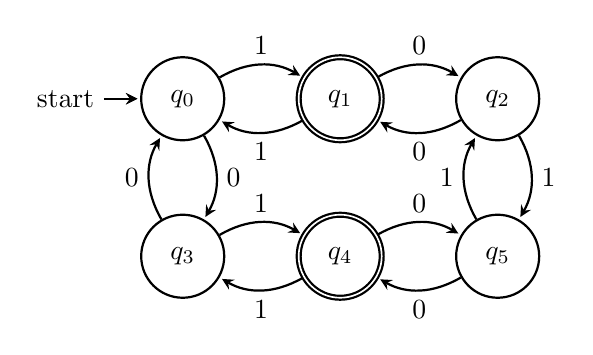
\begin{tikzpicture}[>=stealth, shorten >=1pt, node distance=2.0cm, on grid, auto, state/.append style={minimum size=3em}, thick ]
			\node[state, initial]				(A)               	{$q_0$};
			\node[state, accepting]				(B) [right of=A] 	{$q_1$};
			\node[state]				        (C) [right of=B] 	{$q_2$};
			\node[state]				        (D) [below of=A] 	{$q_3$};
			\node[state, accepting]				(E) [right of=D] 	{$q_4$};
			\node[state]				        (F) [right of=E] 	{$q_5$};
			\path[->] (A) +(-1,0) edge (A)
			
			%Transições:
			%(Partida) edge [tipo da seta] node {simbolo lido} (Destino)
			(A) edge [bend left]  				node 		 {$1$} (B)
			(B) edge [bend left]  				node 		 {$1$} (A)
			(B) edge [bend left]  				node 		 {$0$} (C)
			(C) edge [bend left]  				node 		 {$0$} (B)
			(A) edge [bend left]  				node 		 {$0$} (D)
			(D) edge [bend left]  				node 		 {$0$} (A)
			(C) edge [bend left]  				node 		 {$1$} (F)
			(F) edge [bend left]  				node 		 {$1$} (C)
			(D) edge [bend left]  				node 		 {$1$} (E)
			(E) edge [bend left]  				node 		 {$1$} (D)
			(E) edge [bend left]  				node 		 {$0$} (F)
			(F) edge [bend left]  				node 		 {$0$} (E);
		\end{tikzpicture}
		\caption{Grafo do AFD do Exemplo \ref{exe:LinguagemLAFN1}.}
		\label{fig:Linguagem-AFDM-1}
	\end{figure}
	
	O algoritmo gera a matriz representada na Tabela \ref{tab:AFD-Minimizacao} a seguir, em que a $i$-ésima linha (coluna) representa o estado $q_{i-1}$, e os espaço marcados com $-$ são aqueles não considerados pelo algoritmo, as posições com $X$ representam os estados não equivalentes, e as posições $(i,j)$ em branco representam os estados equivalentes.	
	
	\begin{table}[h]
		\scriptsize
		\centering
		\begin{tabular}{|c|c|c|c|c|c|}
			\hline
			- & X & X &   & X & X\\ \hline
			- & - & X & X &   & X\\ \hline
			- & - & - & X & X & \\ \hline
			- & - & - & - & X & X\\ \hline
			- & - & - & - & - & X\\ \hline
			- & - & - & - & X & -\\ \hline
		\end{tabular}
		\caption{Matriz de equivalência $M$ para o AFD \ref{fig:Linguagem-AFDM-1}.}
		\label{tab:AFD-Minimizacao}
	\end{table}
	
	A partir desta Tabela \ref{tab:AFD-Minimizacao} o Algoritmo \ref{alg:AFD-Quociente} gera as seguintes classes de equivalência: $[q_0] = \{q_0, q_3\}$, $[q_1] = \{q_1, q_4\}$ e $[q_2] = \{q_2, q_5\}$, depois define as transições e o conjunto de estados finais como esboçadas pelo grafo de Transição na Figura \ref{fig:Linguagem-AFDM-2}.
	
	\begin{figure}[h]
		\centering
		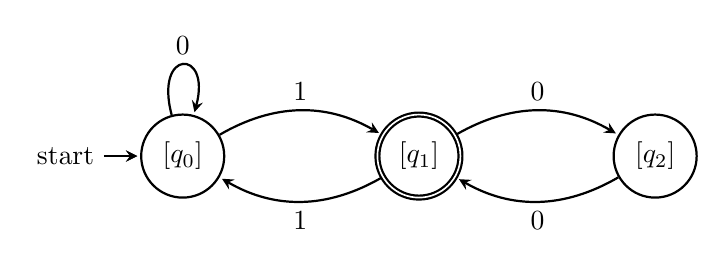
\begin{tikzpicture}[>=stealth, shorten >=1pt, node distance=3.0cm, on grid, auto, state/.append style={minimum size=3em}, thick ]
			\node[state, initial]				(A)               	{$[q_0]$};
			\node[state, accepting]				(B) [right of=A] 	{$[q_1]$};
			\node[state]				        (C) [right of=B] 	{$[q_2]$};
			\path[->] (A) +(-1,0) edge (A)
			
			%Transições:
			%(Partida) edge [tipo da seta] node {simbolo lido} (Destino)
			(A) edge [bend left]  				node 		 {$1$} (B)
			(A) edge [loop above]				node		 {$0$} ( )
			(B) edge [bend left]  				node 		 {$1$} (A)
			(B) edge [bend left]  				node 		 {$0$} (C)
			(C) edge [bend left]  				node 		 {$0$} (B);
		\end{tikzpicture}
		\caption{Grafo do AFD do Exemplo \ref{exe:LinguagemLAFN1}.}
		\label{fig:Linguagem-AFDM-2}
	\end{figure}
\end{example}

Desde que $\delta^*([q], a) = [\delta(q, a)]$ é um caso particular do resultado obtido no Teorema \ref{teo:ExtensaoDeltaEstrela}, e pela condição suficiente e necessária apresentada no Teorema \ref{teo:FinalQuociente}, tem-se que a corretude do Algoritmo \ref{alg:AFD-Quociente} se resumi a demonstrar o teorema a seguir.

\begin{theorem}[Corretude do Algoritmo de Construção do Quociente]
	Seja $A = \langle Q, \Sigma, \delta, q_0, F\rangle$ um AFD. Considerando o Algoritmo \ref{alg:AFD-Quociente} e os índices $j > i$ tem-se que,  $M(i, j)$ está marcado com $X$ se, e somente se, $q_i \not\equiv q_j$.
\end{theorem}

\begin{proof}
	A demonstração fica como exercício ao leitor.
\end{proof}

\subsection{Máquinas de Mealy e Moore}

Os trabalhos iniciais de Mealy \cite{mealy1955} e Moore \cite{moore1956}, além de serem alicerces fundamentais da teoria dos autômatos finitos, também são os trabalhos responsáveis por formalizar o conceito de tradutores finitos ou autômato finito com saída. Diferente dos autômatos sem saída vistos nas seções \ref{subsec:AFD}, \ref{subsec:AFN} e \ref{subsec:LAFN} as máquinas de Mealy e Moore são capazes de apresentar saídas mais complexas que as típicas saídas booleanas (aceita/rejeita) dos AFD, AFN e $\lambda$-AFN. As máquinas de Mealy, por exemplo,  são um modelo matemático simples para definir máquinas de cifras (criptografia), ou seja, máquinas que a partir de um texto de entrada geram um texto cifrado (criptografado) como saída \cite{menezes1998LFA}.

Em termos informais uma autômato com saída pode ser descrito como um máquina que possui duas memórias (somente de leitura), a primeira memória guarda a palavra de entrada usada no funcionamento da máquina, já segunda memória (apenas de escrita) é responsável por armazenar a palavra de saída, sendo essa gerada durante o funcionamento do autômato.

\begin{definition}[Máquina de Mealy]\label{def:MealyMachine}
	Uma máquina de Mealy é uma estrutura $A = \langle Q, \Sigma, \Lambda, \delta, \psi, q_0, \rangle$ onde $Q, \Sigma, \delta$ e $q_0$ são da mesma forma que na Definição \ref{def:AFD}. $\Lambda$ é um alfabeto chamado \textbf{alfabeto de saída} e $\psi: Q \times \Sigma \rightarrow \Lambda^+$ é a função de tradução da máquina de Mealy.
\end{definition}

\begin{example}\label{exe:Mealy1}
	A estrutura $M = \langle \{q_0, q_1\}, \{a, b\}, \{0, 1, 2\}, \delta, \psi, q_0 \rangle$ onde a função de transição é representada pela Tabela \ref{tab:TransicaoMealyEx1} e a função de tradução é representada pela Tabela \ref{tab:TraducaoMealyEx1} a seguir é uma máquina de Mealy.
	
	\begin{table}[h]
		\centering
		\begin{tabular}{c|cc}
			\backslashbox{$Q$}{$\Sigma$} & $a$ & $b$\\ \hline
			$q_0$ & $q_1$ & $q_1$ \\
			$q_1$ & $q_0$ & $q_1$
		\end{tabular}
		\caption{Tabela da Função de transição da Máquina de Mealy do Exemplo \ref{exe:Mealy1}.}
		\label{tab:TransicaoMealyEx1}
	\end{table}
	
	\begin{table*}[h]
		\centering
		\begin{tabular}{c|cc}
			\backslashbox{$Q$}{$\Sigma$} & $a$ & $b$\\ \hline
			$q_0$ & $11$ & $20$ \\
			$q_1$ & $12$ & $02$ 
		\end{tabular}
		\caption{Tabela da Função de tradução da Máquina de Mealy do Exemplo \ref{exe:Mealy1}.}
		\label{tab:TraducaoMealyEx1}
	\end{table*}
\end{example}

Pode-se utilizar a ideia de grafo de transição para representar visualmente as máquinas de Mealy a única diferença que esta representação terá em relação aos grafos que representam os AFD, é que as arestas que ligam dois vértices $q_i$ e $q_j$ serão rotuladas com pares $(a, x) \in \Sigma \times \Lambda$ representando assim simultaneamente as funções $\delta(q_i, a) = q_j$ e $\psi(q_i, a) = x$.

\begin{example}\label{exe:MaquinaMealyGrafo1}
	A representação do grafo de transição da máquina de Mealy do Exemplo \ref{exe:Mealy1} é como se segue.
	
	\begin{figure}[h]
		\centering
		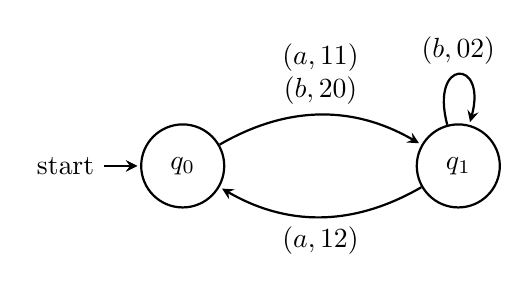
\begin{tikzpicture}[>=stealth, shorten >=1pt, node distance=3.5cm, on grid, auto, state/.append style={minimum size=3em}, thick ]
			\node[state, initial]							(A)               	{$q_0$};
			\node[state]									(B) [right of=A] 	{$q_1$};
			\path[->] (A) +(-1,0) edge (A)
			
			%Transições:
			%(Partida) edge [tipo da seta] node {simbolo lido} (Destino)
			(A) edge [bend left]  				node [align=center]   {$(a, 11)$\\$(b, 20)$} (B)
			(B) edge [bend left]  				node    			  {$(a, 12)$} (A)
			(B) edge [loop above]				node    			  {$(b, 02)$} ( );
		\end{tikzpicture}
		\caption{Representação da máquina de Mealy do Exemplo \ref{exe:Mealy1}.}
		\label{fig:MaquinaMealy1}
	\end{figure}
\end{example}

Note que a máquina de Mealy traduz (ou associa) cada transição da máquina a um símbolo do alfabeto de saída, ou seja, cada movimento no processo de computação da máquina é traduzido na saída da mesma. Obviamente $\widehat{\delta}$ é definido da mesma forma que para os AFD, sendo assim basta agora estender a função $\psi$ para que a máquina de Mealy possa de fato ser vista como um tradutor finito, e isto será feito a seguir.

\begin{definition}[Extensão da função $\psi$]
	Seja $A = \langle Q, \Sigma, \Lambda, \delta, \psi, q_0\rangle$ uma máquina de Mealy a função $\psi$ é estendida para a função $\widehat{\psi} : Q \times \Sigma^* \rightarrow \Lambda^*$ usando recursividade como se segue.
	
	\begin{eqnarray}\label{eq:ExtensaoDaFuncaoDetraducaoMealy}
		\widehat{\psi}(q, \lambda)& = & \lambda \\
		\widehat{\psi}(q, wa)& = & \widehat{\psi}(q, w)\psi(\widehat{\delta}(q, w), a)
	\end{eqnarray}
\end{definition} 

\begin{example}
	Considerando a máquina de Mealy do Exemplo \ref{exe:Mealy1} a tradução da palavra $bab$ a partir do estado $q_1$ é dada seguinte forma,
	\begin{eqnarray*}
		\widehat{\psi}(q_1, bab) & = & \widehat{\psi}(q_1, ba)\psi(\widehat{\delta}(q_1, ba), b)\\
		& = & \widehat{\psi}(q_1, b)\psi(\widehat{\delta}(q_1, b), a)\psi(\widehat{\delta}(q_1, ba), b)\\
		& = & \widehat{\psi}(q_1, \lambda)\psi(\widehat{\delta}(q_1, \lambda), b)\psi(\widehat{\delta}(q_1, b), a)\psi(\widehat{\delta}(q_1, ba), b)\\
		& = & \lambda 021220\\
		& = & 021220
	\end{eqnarray*}
\end{example}

\begin{remark}
	Pode-se interpretar que as funções $\psi$ e $\widehat{\psi}$ escrevem na fita de saída da máquina, isto é, na memória adicional de escrita que tais máquinas possuem.
\end{remark}

Diferentemente dos AFD, AFN e $\lambda$-AFN o conjunto saída de qualquer máquina de Mealy não visto como uma linguagem aceita pela máquina, em vez disso, ela é vista como a linguagem traduzida pela máquina.

\begin{definition}[Linguagem Traduzia - Máquina de Mealy]
	Dado uma máquina de Mealy $A = \langle Q, \Sigma, \Lambda, \delta, \psi, q_0\rangle$ a linguagem traduzida de $A$, denotado por $TRAD(A)$, é o conjunto de todas as traduções das palavras $w \in \Sigma^*$ realizadas a partir do estado inicial $q_0$, ou seja, tem-se que:
	\begin{equation}
		TRAD(A) = \{\widehat{\psi}(q_0, w)  \mid w \in \Sigma^*\}
	\end{equation}
\end{definition}

Em contrapartida as máquinas de Mealy, que como já dito, traduzem cada transição da máquina em um fragmento da palavra de saída, existem as máquina de Moore, nomeadas em homenagem a Edward F. Moore (1925-2003) que as propôs em seu seminal artigo \cite{moore1956}, tais máquinas não traduzem as transições em prefixos da palavras de saída, em vez disso, cada estado da máquina é mapeado em um símbolo do alfabeto de saída.

\begin{definition}[Máquina de Moore]\label{def:MooreMachine}
	Uma máquina de Moore é uma estrutura $A = \langle Q, \Sigma, \Lambda, \delta, \Phi, q_0\rangle$ onde $Q, \Sigma, \delta$ e $q_0$ são da mesma forma que na Definição \ref{def:AFD}. $\Lambda$ é um alfabeto chamado \textbf{alfabeto de saída} e $\Phi: Q \rightarrow \Lambda^+$ é a função de escrita dos estado da máquina de Moore.
\end{definition}

\begin{example}\label{exe:Moore1}
	A estrutura $M = \langle \{q_0, q_1, q_3\}, \{a, b\}, \{x, y, z\}, \delta, \Phi, q_0 \rangle$ onde a função de transição é esboçada pela Tabela \ref{tab:TransicaoMoore1} a seguir, sendo a função de escrita dos estados é definida como: $\Phi(q_0) = xy, \Phi(q_1) = yz$ e $\Phi(q_2) = zx$. É uma máquina de Moore.
	
	\begin{table}[h]
		\centering
		\begin{tabular}{c|cc}
			\backslashbox{$Q$}{$\Sigma$} & a & b\\ \hline
			$q_0$ & $q_1$ & $q_2$ \\
			$q_1$ & $q_1$ & $q_2$ \\
			$q_2$ & $q_0$ & $q_2$ 
		\end{tabular}
		\caption{Tabela de transição para a máquina de Moore do Exemplo \ref{exe:Moore1}.}
		\label{tab:TransicaoMoore1}
	\end{table}
\end{example}

Similar aos AFD pode-se utilizar a ideia de grafo de transição para representar visualmente as máquinas de Moore a única diferença que esta representação terá em relação aos grafos que representam os AFD, é que os vértices serão rotulados por pares $(q, w) \in Q \times \Lambda$ e $q_j$ em que $\Phi(q) = w$.

\begin{figure}[h]
	\centering
	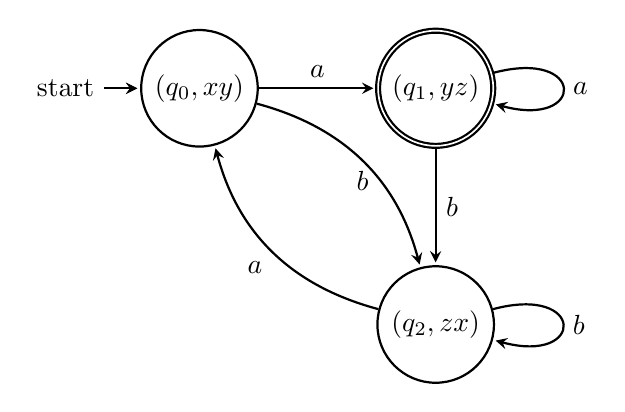
\begin{tikzpicture}[>=stealth, shorten >=1pt, node distance=3.0cm, on grid, auto, state/.append style={minimum size=1em}, thick ]
		\node[state, initial]							(A)               	{$(q_0, xy)$};
		\node[state, accepting]							(B) [right of=A] 	{$(q_1, yz)$};
		\node[state]									(C) [below of=B] 	{$(q_2, zx)$};
		\path[->] (A) +(-1,0) edge (A)
		
		%Transições:
		%(Partida) edge [tipo da seta] node {simbolo lido} (Destino)
		(A)	edge			  				node   				  {$a$} (B)
		(A) edge [bend left]  				node [below]		  {$b$} (C)
		(B) edge [loop right]				node				  {$a$} ( )
		(B)	edge			  				node   				  {$b$} (C)
		(C) edge [bend left]  				node   				  {$a$} (A)
		(C) edge [loop right]				node				  {$b$} ( );
	\end{tikzpicture}
	\caption{Representação da máquina de Moore do Exemplo \ref{exe:Mealy1}.}
	\label{fig:MaquinaMoore1}
\end{figure}

\begin{example}\label{exe:MaquinaMooreGrafo1}
	A representação do grafo de transição da máquina de Mealy do Exemplo \ref{exe:Moore1} pode ser observada na Figura \ref{fig:MaquinaMoore1}.
\end{example}

\begin{remark}
	Note que para qualquer $w \in \Sigma^*$ tem-se que $\Phi(\widehat{\delta}(q_0,w))$ expressa a saída da máquina de Moore para a palavra $w$.
\end{remark}

Para que as máquinas de Moore possam ser vistas como tradutores é necessário apresentar uma função de tradução para tais máquinas, sendo esta apresentada a seguir.

\begin{definition}[Função de tradução das máquinas de Moore]
	Dado uma máquina de Moore $A = \langle Q, \Sigma, \Lambda, \delta, \Phi, q_0\rangle$ a função de tradução $\widehat{\Phi} : Q \times \Sigma^* \rightarrow \Lambda^*$ é definida por recursão como se segue.
	
	\begin{eqnarray}\label{eq:ExtensaoDaFuncaoDetraducaoMoore}
		\widehat{\Phi}(q, \lambda)& = & \lambda \\
		\widehat{\Phi}(q, wa)& = & \widehat{\Phi}(\widehat{\delta}(q, w))\Phi(\widehat{\delta}(q, wa))
	\end{eqnarray}
\end{definition}

\begin{remark}
	Pode-se assim como para o caso das máquinas de Mealy considerar que a função de tradução das máquinas de Moore, isto é, a função $\widehat{\Phi}$ escreve a memória de escrita da máquina.
\end{remark}

\begin{definition}[Linguagem Traduzia - Máquina de Moore]
	Dado uma máquina de Moore $A = \langle Q, \Sigma, \Lambda, \delta, \Phi, q_0\rangle$ a linguagem traduzida de $A$, denotado por $TRAD(A)$, é o conjunto de todas as traduções das palavras $w \in \Sigma^*$ realizadas a partir do estado inicial $q_0$, ou seja, tem-se que:
	\begin{equation}
		TRAD(A) = \{\widehat{\Phi}(q_0, w) \mid  w \in \Sigma^*\}
	\end{equation}
\end{definition}

O leitor atento deve ter notado pelas definições que as traduções feitas pelas máquinas de Mealy e Moore, apresentam a propriedade de involução sobre a palavra vazia. Os próximos resultados apresentam uma forte relação entre as máquinas de Mealy e Moore.

\begin{theorem}[Transformação Moore-Mealy]\label{teo:Moore-Mealy}
	Dado uma linguagem $L \subseteq \Lambda^*$. Se $L = TRAD(N)$ para alguma máquina de Moore $N$,  então existe uma máquina de Mealy $M$ tal que $L = TRAD(M)$.
\end{theorem}

\begin{proof}
	Suponha que $L = TRAD(N)$ para alguma máquina de Moore $N = \langle Q, \Sigma, \Lambda, \delta, \Phi, q_0\rangle$, agora defina uma máquina de Mealy $M = \langle Q, \Sigma, \Lambda, \delta, \psi, q_0\rangle$, onde para todo $(q, a) \in Q \times \Sigma$ é definido que:
	\begin{eqnarray}\label{eq:ConversaoMoore-Mealy}
		\psi(q, a) & = & \Phi(\delta(q, a))
	\end{eqnarray}
	Agora será mostrado por indução sobre o tamanho das palavras que para todo $w \in \Sigma^+$ que que as traduções de $M$ e $N$ são iguais, ou seja, será mostrado que $\widehat{\Phi}(q_0, w) = \widehat{\psi}(q_0, w)$.
	\begin{itemize}
		\item \textbf{Base da indução:} Quando $|w| = 0$ é trivial da própria definição de $\widehat{\Phi}$ e $\widehat{\psi}$.
		\item \textbf{Hipótese indutiva (HI)}: Suponha que para todo $|w| = n$ com $n \geq 0$ tem-se que $\Phi(q_0, w) = \psi(q_0, w)$.
		\item \textbf{Passo indutivo}: Dado $|w| = ua$ com $u \in \Sigma^*$ tal que $|u| \geq 0$ e $a \in \Sigma$ tem-se que,
		
		\begin{eqnarray*}
			\widehat{\Phi}(q_0, w) & = & \widehat{\Phi}(q_0, ua)\\
			& = & \widehat{\Phi}(q_0, u)\Phi(\widehat{\delta}(q_0, ua))\\
			& \stackrel{\textbf{(HI)}}{=} & \widehat{\psi}(q_0, u)\Phi(\widehat{\delta}(q_0, ua))\\
			& = & \widehat{\psi}(q_0, u)\Phi(\delta(\widehat{\delta}(q_0, u), a))\\
			& \stackrel{Eq. \ \ref{eq:ConversaoMoore-Mealy}}{=} & \widehat{\psi}(q_0, u)\psi(\widehat{\delta}(q_0, u), a)\\
			& = & \widehat{\psi}(q_0, ua)\\ 
			& = & \widehat{\psi}(q_0, w)
		\end{eqnarray*}
	\end{itemize}
	Consequentemente, $TRAD(N) = TRAD(M)$ e, portanto, $L = TRAD(M)$.
\end{proof}

\begin{theorem}[Transformação Mealy-Moore]\label{teo:Mealy-Moore}
	Dado uma linguagem $L \subseteq \Lambda^*$. Se $L = TRAD(N)$ para alguma máquina de Mealy $N$,  então existe uma máquina de Moore $M$ tal que $L = TRAD(M)$.
\end{theorem}

\begin{proof}
	Similar ao raciocínio da demonstração do Teorema \ref{teo:Moore-Mealy}, e ficará como exercício ao leitor.
\end{proof}

\begin{remark}
	As definições dadas aqui não apresentam o conceito de estado final, para leitores interessados em máquinas de Mealy e Moore com estados finais ver \cite{menezes1998LFA}.
\end{remark}

\section{A Notação Matricial}\label{sec:NotacaoMatricial}

Escrever depois...

\section{Expressões Regulares}\label{sec:ExpressaoRegulares}

Até agora as linguagens foram vistas sobre a ótica das máquinas de computação, isto é, sobre a perspectiva dos autômatos finitos, em tal perspectiva as linguagens são vistas como sendo conjuntos de palavras sobre os quais as máquinas tinha a tarefa de reconhecer seus elementos. 

Neste seção será apresentada uma nova visão de aspecto mais algébrico para as linguagens, essa nova visão foi introduzida por Kleene em seu seminal \textit{paper} ``\textit{Representation of events in nerve nets and finite automata}'' \cite{kleene1951}, tal perspectiva consiste em um sistema formal (com sintaxe e semântica) chamado de expressões  regulares, a seguir é formalizado a sintaxe das expressões regulares.

\begin{definition}[Conjunto das Expressões Regulares -- Sintaxe]\label{def:ExpRegularesSintaxe}
	Seja $\Sigma$ uma alfabeto, o conjunto de todas as expressões regulares sobre $\Sigma$, denotado por $Exp_\Sigma$, é o conjunto indutivamente gerado pelas seguintes regras.
	\begin{itemize}
		\item[ ]\textbf{(B)ase}: $\emptyset, \lambda$ e cada $a \in \Sigma$, são expressões regulares\footnote{As expressões regulares da base costumam ser chamadas de expressões regulares primitivas.}.
		\item[ ]\textbf{(P)asso indutivo}:  Se $r_1, r_2 \in Exp_\Sigma$, então $r_1 + r_2, r_1 \cdot r_2, r_1^*, (r_1) \in Exp_\Sigma$.
		\item[ ]\textbf{(F)echo}: $Exp_\Sigma$ é exatamente o conjunto dos elementos obtidos a partir \textbf{(B)} ou usando-se uma quantidade finita (podendo ser nula) de aplicações de \textbf{(P)}.
	\end{itemize}
\end{definition}

No que diz respeito as expressões regulares é comum assumir que $+, \cdot, (, ), ^* \notin \Sigma$, assim uma expressão regular nem sempre é uma palavra sobre $\Sigma$, em geral os símbolos $+$ e $\cdot$ são lidos como soma e produto \cite{carroll1989}. Além disso, como dito em \cite{benjaLivro2010} se $r_1, r_2 \in Exp_\Sigma$, então costuma-se escrever $r_1r_2$ em vez de $r_1\cdot r_2$.

\begin{remark}
	Também é possível encontrar referência em que o termo expressão regular seja trocado para álgebra de Kleene.
\end{remark}

\begin{example}
	Considerando o alfabeto $\{0,1\}$ tem-se que $(1 + 1)0, 01 \in Exp_\Sigma$. Essa afirmação pode ser verificada construindo tais palavras facilmente, basta pela regra \textbf{(B)} tem-se que  $0$ e $1$ são expressões regulares primitivas, assim usando a regra \textbf{(P)} pode-se construir as expressões $1 + 1$ e $01$, agora aplicando novamente a regra \textbf{(P)} sobre a expressão $1 + 1$ pode-se gerar a expressão $(1 + 1)$, finalmente, aplicando \textbf{(P)} novamente obtem-se a expressão $(1+1)0$ e isso mostra que de fato $(1 + 1)0, 01 \in Exp_\Sigma$.
\end{example}

\begin{example}
	Considerando o alfabeto $\{a, b, c\}$ tem-se que $a(\emptyset + (bc^*)) \in Exp_\Sigma$. Essa afirmação pode ser verificada construindo tal palavra, uma vez que, $a, b$ e $c$ são expressões regulares primitivas aplicando o passo \textbf{(B)} varias vezes será obtida a expressão regular $a(\emptyset + (bc^*)$.
\end{example}

A seguir será formalizado o conceito de semântica para as expressões regulares, sendo que tal semântica pode ser visto como uma \textbf{semântica denotacional}\footnote{Uma semântica denotacional é aquela em que as funções de valoração usadas, são funções que mapeiam palavras da linguagem para funções parciais que representam o comportamento dos programas.} \cite{scott1971}, que apresenta significado as operações de soma e multiplicação.

\begin{definition}[Semântica das Expressão Regulares]\label{def:ExpRegularesSemantica}
	Seja $Exp_\Sigma$ o conjunto das expressões regulares sobre $\Sigma$,  a semântica (ou interpretação) de $Exp_\Sigma$ é uma função $\mathcal{L}: Exp_\Sigma \rightarrow \wp(\Sigma^*)$ definida recursivamente para todo $r, r_1, r_2  \in Exp_\Sigma$ pelas seguintes regras.
	\begin{itemize}
		\item[(i)] Se $r \in \Sigma \cup \{\lambda\}$, então $\mathcal{L}(r) = \{r\}$.
		\item[(ii)] Se $r = \emptyset$, então $\mathcal{L}(r) = \emptyset$.
		\item[(iii)] Se $r = r_1 + r_2$, então $\mathcal{L}(r) = \mathcal{L}(r_1) \cup \mathcal{L}(r_2)$.
		\item[(iv)] Se $r = r_1 \cdot r_2$, então $\mathcal{L}(r) = \mathcal{L}(r_1)\mathcal{L}(r_2)$.
		\item[(v)] Se $r = r_1^*$, então $\mathcal{L}(r) = (\mathcal{L}(r_1))^*$.
		\item[(vi)] Se $r = (r_1)$, então $\mathcal{L}(r) = (\mathcal{L}(r_1))$.	
	\end{itemize}
\end{definition}

Agora como explicado em \cite{carroll1989}, para a valoração de expressões regulares não primitivas, é necessário que seja seguido a precedência dos operadores no momento de combinar as linguagens, sendo tal precedência no sentido de maior precedência para a menor formada pela seguinte ordem: fecho de Kleene, concatenação e união.

\begin{remark}
	Vale destacar que como na aritmética convencional os parênteses mudam a precedência dos conectivos anteriores, e deve ser avaliados dos mais internos para os mais externos.
\end{remark}

\begin{note}
	A valoração pode vim a gerar situações como $(L)$ onde $L \subseteq \Sigma^*$, neste caso será escrito simplesmente $L$ vem vez de $(L)$.
\end{note}

\begin{example}\label{exe:ValoracaoExpressao1}
	Dado o alfabeto $\{0,1\}$ e $(00)^* \in Exp_\Sigma$ tem-se que:
	\begin{eqnarray*}
		\mathcal{L}((00)^*) & = & (\mathcal{L}((00)))^*\\
		& = & ((\mathcal{L}(00)))^*\\
		& = & ((\mathcal{L}(0)\mathcal{L}(0)))^*\\
		& = & ((\{0\}\{0\}))^*\\
		& = & ((\{00\}))^*\\
		& = & (\{00\})^*\\
		& = & \{00\}^*\\
		& = & \{\lambda, 00, 0000, 000000, 00000000, \cdots\}
	\end{eqnarray*}
	ou seja, a valoração da expressão regular $(00)^*$ consiste da linguagem de todas as palavras $w$ sobre o alfabeto $\{0,1\}$ sem nenhum 1 e que o tamanho seja par, isto é, $|w| = 2k$ para algum $k \in \mathbb{N}$.
\end{example}


\begin{example}\label{exe:ValoracaoExpressao2}
	Dado o alfabeto $\{0,1\}$ e $(0 + 1^*)0 \in Exp_\Sigma$ tem-se que:
	\begin{eqnarray*}
		\mathcal{L}((0 + 1^*)0 ) & = & \mathcal{L}((0 + 1^*))\mathcal{L}(0)\\
		& = & (\mathcal{L}(0 + 1^*))\{0\}\\
		& = & (\mathcal{L}(0) \cup  \mathcal{L}(1^*))\{0\}\\
		& = & (\mathcal{L}(0) \cup  (\mathcal{L}(1))^*)\{0\}\\
		& = & (\{0\} \cup \{1\}^*)\{0\}\\
		& = & (\{0\} \cup \{\lambda, 1, 11, 111, 1111, \cdots\})\{0\}\\
		& = & \{\lambda, 0, 1, 11, 111, 1111, \cdots\}\{0\}\\
		& = & \{0, 00, 10, 110, 1110, 11110, \cdots \}
	\end{eqnarray*}
	ou seja, a valoração da expressão regular $\{0,1\}$ e $(0 + 1^*)0$ é exatamente a linguagem de todas as palavras $w$ sobre o alfabeto $\{0,1\}$  sendo que $w = 0^m$ ou $w = 1^n0$ com $m,n \in \mathbb{N}$ tal que $1 \leq m \leq 2$ e $n \geq 1$.
\end{example}

\begin{example}
	Dado o alfabeto $\{a,b,c\}$ e a expressão $((ab)^* + c)\emptyset \in Exp_\Sigma$ tem-se que:
	\begin{eqnarray*}
		\mathcal{L}(((ab)^* + c) \emptyset) & = & \mathcal{L}(((ab)^* + c))\mathcal{L}(\emptyset)\\
		& = & (\mathcal{L}((ab)^* + c))\emptyset\\
		& = & (\mathcal{L}((ab)^*) \cup \mathcal{L}(c))\emptyset\\
		& = & ((\mathcal{L}((ab)))^* \cup \{c\})\emptyset\\
		& = & (((\mathcal{L}(ab)))^* \cup \{c\})\emptyset\\
		& = & (((\mathcal{L}(a)\mathcal{L}(b)))^* \cup \{c\})\emptyset\\
		& = & (((\{a\}\{b\}))^* \cup \{c\})\emptyset\\
		& = & (((\{ab\}))^* \cup \{c\})\emptyset\\
		& = & ((\{ab\})^* \cup \{c\})\emptyset\\
		& = & (\{ab\}^* \cup \{c\})\emptyset\\
		& = & (\{\lambda, ab, abab, ababab, \cdots\} \cup \{c\})\emptyset\\
		& = & (\{\lambda, c, ab, abab, ababab, \cdots\})\emptyset\\
		& = & \{\lambda, c, ab, abab, ababab, \cdots\}\emptyset\\
		& = & \{\lambda, c, ab, abab, ababab, \cdots\}
	\end{eqnarray*}
	portanto, a valoração da expressão regular $((ab)^* + c)\emptyset$ é exatamente a linguagem de todas as palavras $w$ sobre o alfabeto $\{a,b,c\}$  onde $w = c^m$ ou $w = (ab)^n$ com $m,n \in \mathbb{N}$ tal que $m \leq 1$ e $n \geq 1$.
\end{example}

\begin{definition}
	Duas expressões regulares $r_1, r_2 \in Exp_\Sigma$ são dita equivalentes, denotado por $r_1 \equiv r_2$, sempre que $\mathcal{L}(r_1) = \mathcal{L}(r_2)$.
\end{definition}

\begin{example}
	Dada a expressão $00 + (1^*0)$ note que:
	\begin{eqnarray*}
		\mathcal{L}(00 + (1^*0)) & = &\mathcal{L}(00) \cup \mathcal{L}((1^*0))\\
		& = & \mathcal{L}(0)\mathcal{L}(0) \cup (\mathcal{L}(1^*0))\\
		& = & \mathcal{L}(0)\mathcal{L}(0) \cup (\mathcal{L}(1^*)\mathcal{L}(0))\\
		& = & \mathcal{L}(0)\mathcal{L}(0) \cup ((\mathcal{L}(1))^*\mathcal{L}(0))\\
		& = & \{0\}\{0\} \cup ((\{1\})^*\{0\})\\
		& = & \{0\}\{0\} \cup (\{1\}^*\{0\})\\
		& = & \{0\}\{0\} \cup (\{\lambda, 1, 11, 111, 1111, \cdots\}\{0\})\\
		& = & \{0\}\{0\} \cup (\{0, 10, 110, 1110, 11110, \cdots\})\\
		& = & \{0\}\{0\} \cup \{0, 10, 110, 1110, 11110, \cdots\}\\
		& = & \{00\} \cup \{0, 10, 110, 1110, 11110, \cdots\}\\
		& = & \{0, 00, 10, 110, 1110, 11110, \cdots\}
	\end{eqnarray*}
	logo, tal expressão é equivalente a expressão  $\equiv (0 + 1^*)0$ apresentada no Exemplo \ref{exe:ValoracaoExpressao2}. 
\end{example}

\begin{proposition}
	Se $r_1, r_2, r_3 \in Exp_\Sigma$, então $r_1 (r_2 + r_3) \equiv r_1r_2 + r_1r_3$.
\end{proposition}

\begin{proof}
	Assuma que $r_1, r_2, r_3 \in Exp_\Sigma$, logo tem-se que;
	\begin{eqnarray*}
		\mathcal{L}(r_1 (r_2 + r_3)) & = & \mathcal{L}(r_1)\mathcal{L}((r_2 + r_3))\\
		& = & \mathcal{L}(r_1)(\mathcal{L}(r_2 + r_3))\\
		& = & \mathcal{L}(r_1)(\mathcal{L}(r_2) \cup  \mathcal{L}(r_3))\\ 
		& = & \mathcal{L}(r_1)(\mathcal{L}(r_2) \cup  \mathcal{L}(r_3))\\ 
		& = & \mathcal{L}(r_1)\mathcal{L}(r_2) \cup  \mathcal{L}(r_1)\mathcal{L}(r_3)\\ 
		& = & \mathcal{L}(r_1r_2 + r_1r_3)
	\end{eqnarray*}
	O que conclui a prova.
\end{proof}

Agora será mostrado qual a classe (ou tipo) de linguagens definidas por expressões regulares, ou seja, agora será mostrado a que classe pertencem as linguagens fruto da valoração das expressões regulares.

\begin{theorem}[Transformação de expressões regulares para AFN]\label{teo:Exp-AFN}
	Se $L = \mathcal{L}(r)$ para alguma expressão regular $r$, então existe um $\lambda$-AFN $A$ tal que $L = \mathcal{L}(A)$.
\end{theorem}

\begin{proof}
	Suponha que $L = \mathcal{L}(r)$ para alguma expressão regular $r$, agora por indução sobre o número de operadores em $r$ será mostrado que existe um $\lambda$-AFN $A$ tal que $L = \mathcal{L}(A)$.
	
	\begin{itemize}
		\item \textbf{Base da indução}:
		
		Para as expressões regulares $r$ com $0$ operadores, isto é, $r = \lambda$ ou $r = \emptyset$ ou $r = a$ para $a \in \Sigma$ considere os seguintes $\lambda$-AFN.
		
		\begin{figure}[h]
			\centering
			\subfloat[$\lambda$-AFN $A_\lambda$.]{
				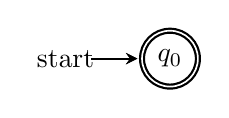
\begin{tikzpicture}[>=stealth, shorten >=1pt, node distance=3cm, on grid,
					auto, state/.append style={minimum size=2em}, thick ]
					\node[state,initial, accepting]   (A)               {$q_0$};
					
					
					\path[->] (A) +(-1,0) edge (A)
					
					%Transições:
					%(Partida) edge [tipo da seta] node {simbolo lido} (Destino)
					;
				\end{tikzpicture}
				\label{Ima:Automato-A}
			}\quad\quad\quad
			\subfloat[$\lambda$-AFN $A_\emptyset$.]{
				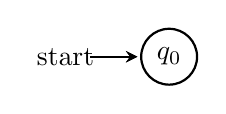
\begin{tikzpicture}[>=stealth, shorten >=1pt, node distance=3cm, on grid,
					auto, state/.append style={minimum size=2em}, thick ]
					\node[state,initial]   (A)               {$q_0$};
					
					
					\path[->] (A) +(-1,0) edge (A)
					
					%Transições:
					%(Partida) edge [tipo da seta] node {simbolo lido} (Destino)
					;
				\end{tikzpicture}
				\label{Ima:Automato-B}
			}\quad\quad\quad
			\subfloat[$\lambda$-AFN $A_a$.]{
				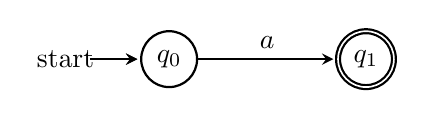
\begin{tikzpicture}[>=stealth, shorten >=1pt, node distance=2.5cm, on grid,
					auto, state/.append style={minimum size=2em}, thick ]
					\node[state,initial]    (A)               {$q_0$};
					\node[state, accepting] (B)[right of=A]   {$q_1$};
					
					
					\path[->] (A) +(-1,0) edge (A)
					
					%Transições:
					%(Partida) edge [tipo da seta] node {simbolo lido} (Destino)
					(A) edge 				            node {$a$}           (B);
				\end{tikzpicture}
				\label{Ima:Automato-C}
			}%
			\caption{Os três $\lambda$-AFN básicos para as expressões regulares primitivas.}
			\label{fig:AFD-basicos}
		\end{figure}
		
		Claramente tem-se que $\mathcal{L}(\lambda) = \mathcal{L}(A_\lambda), \mathcal{L}(\emptyset) = \mathcal{L}(A_\emptyset)$ e $\mathcal{L}(a) = \mathcal{L}(A_a)$ para todo $a \in \Sigma$.
		
		
		\item \textbf{Hipótese indutiva (HI)}:
		
		Suponha que para toda $r \in Exp_\Sigma$ com $n$ operadores tal que $n \geq 0$ existe um $\lambda$-AFN $A = \langle Q_r, \Sigma, \delta_N^r, q_0^r, \{q_f^r\}\rangle$ tal que $\mathcal{L}(r) = \mathcal{L}(A^r)$. Para fins de representação considere que tal $\lambda$-AFN $A^r$ tem a forma a seguir.
		
		\begin{figure}[h]
			\centering
			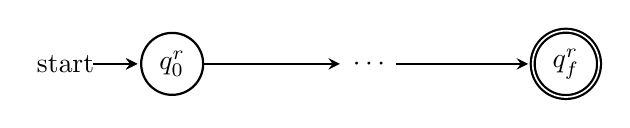
\begin{tikzpicture}[>=stealth, shorten >=1pt, node distance=2.5cm, on grid,
				auto, state/.append style={minimum size=2em}, thick ]
				\node[state,initial]   (A)               {$q_0^r$};
				\node				   (B)[right of=A]   {$\cdots$};
				\node[state, accepting](C)[right of=B]   {$q_f^r$};
				
				
				\path[->] (A) +(-1,0) edge (A)
				
				%Transições:
				%(Partida) edge [tipo da seta] node {simbolo lido} (Destino)
				(A) edge 				            node { }         (B)
				(B) edge 				            node { }         (C);
			\end{tikzpicture}
			\caption{$\lambda$-AFN $A^r$ para uma expressão $r$ genérica com $n$ operadores.}
			\label{Ima:Automato-D}
		\end{figure}
		
		\item \textbf{Passo indutivo}:
		
		
		Agora dado uma expressão regular $r$ com $n + 1$ operadores tal que $n \geq 0$, existe três (e apenas três) casos possíveis para a forma de $r$. 
		
		\begin{itemize}
			\item[\textbf{1º}] \textbf{Caso}: $r = r_1 + r_2$, assim respectivamente $r_1$ e $r_2$ possuem $k_1$ e $k_2$ operadores tais que $k_1 + k_2 = n$, obviamente $k_1, k_2 \geq 0$ e, portanto, por \textbf{(HI)} tem-se que existem $A^{r_1} = \langle Q_{r_1}, \Sigma, \underline{\delta_N}^{r_1}, q_0^{r_1}, \{q_f^{r_1}\}\rangle$ e $A^{r_2} = \langle Q_{r_2}, \Sigma, \underline{\delta_N}^{r_2}, q_0^{r_2}, \{q_f^{r_2}\}\rangle$  tal que $\mathcal{L}(r_1) = \mathcal{L}(A^{r_1})$ e $\mathcal{L}(r_2) = \mathcal{L}(A^{r_2})$, agora pode-se criar um novo $\lambda$-AFN $A^r = \langle Q_{r_1} \cup Q_{r_2} \cup \{q_0\}, \Sigma, \underline{\delta_N}^r, q_0, \{q_f^{r_1}, q_f^{r_2}\}\rangle$ onde,
			\begin{eqnarray*}
				\underline{\delta_N}^r(q, a) & = & 
				\left\{\begin{array}{ll}	
					\underline{\delta_N}^{r_1}(q, a), & \hbox{se } q \in Q_{r_1}\\	
					\underline{\delta_N}^{r_2}(q, a), & \hbox{se } q \in Q_{r_2}\\
					\{q_0^{r_1}, q_0^{r_2}\}, & \hbox{se } q = q_0, a = \lambda\\
					\emptyset, & \hbox{qualquer outro caso}
				\end{array}\right.
			\end{eqnarray*}
			Para fins de representação considere que tal $\lambda$-AFN $A^r$ tem a forma a seguir.
			
			\begin{figure}[h]
				\centering
				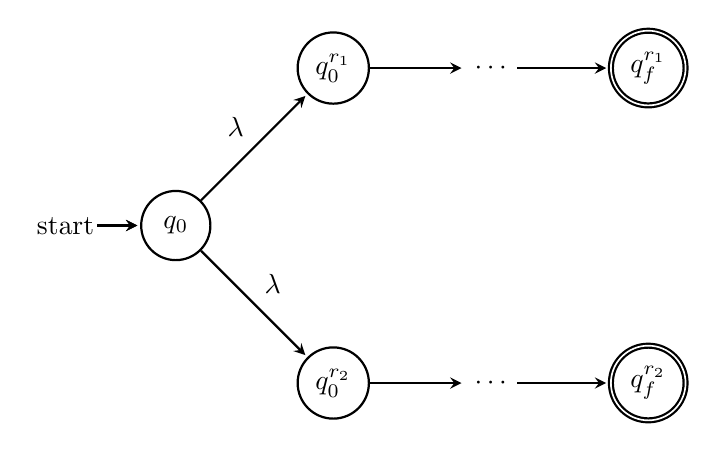
\begin{tikzpicture}[>=stealth, shorten >=1pt, node distance=2.0cm, on grid,
					auto, state/.append style={minimum size=2.5em}, thick ]
					\node[state,initial]   (A)               {$q_0$};
					\node				   (B)[right of=A]   {};
					\node[state]		   (C)[above of=B]   {$q_0^{r_1}$};
					\node				   (C1)[right of=C]	 {$\cdots$};
					\node[state, accepting](C2)[right of=C1] {$q_f^{r_1}$};
					\node[state]		   (D)[below of=B]   {$q_0^{r_2}$};
					\node				   (D1)[right of=D]	 {$\cdots$};
					\node[state, accepting](D2)[right of=D1] {$q_f^{r_2}$};
					
					
					\path[->] (A) +(-1,0) edge (A)
					
					%Transições:
					%(Partida) edge [tipo da seta] node {simbolo lido} (Destino)
					(A) edge 				            node {$\lambda$}         (C)
					(A) edge 				            node {$\lambda$}         (D)
					(C) edge 				            node {}			         (C1)
					(C1) edge 				            node {}			         (C2)
					(D) edge 				            node {}			         (D1)
					(D1) edge 				            node {}			         (D2);
				\end{tikzpicture}
				\caption{$\lambda$-AFN $A^r$ para uma expressão $r_1 + r_2$.}
				\label{Ima:Automato-E}
			\end{figure}
			
			Agora note que para todo $w \in \Sigma^*$ tem-se que,
			\begin{eqnarray*}
				w \in \mathcal{L}(r) & \Longleftrightarrow & w \in \mathcal{L}(r_1 + r_2)\\
				& \Longleftrightarrow & w \in \mathcal{L}(r_1) \cup  \mathcal{L}(r_2)\\
				& \Longleftrightarrow & w \in \mathcal{L}(r_1) \text{ ou } w \in \mathcal{L}(r_2)\\
				& \Longleftrightarrow & \widehat{\underline{\delta_N}^{r_1}}(q_0^{r_1}, w) \cap \{q_f^{r_1}\} \neq \emptyset \text{ ou } \widehat{\underline{\delta_N}^{r_2}}(q_0^{r_2}, w) \cap \{q_f^{r_2}\} \neq \emptyset\\
				& \Longleftrightarrow & \widehat{\underline{\delta_N}}(q_0, w) \cap \{q_f^{r_1}\} \neq \emptyset \text{ ou } \widehat{\underline{\delta_N}}(q_0, w) \cap \{q_f^{r_2}\} \neq \emptyset\\
				& \Longleftrightarrow & \widehat{\underline{\delta_N}}(q_0, w) \cap \{q_f^{r_1}, q_f^{r_2}\} \neq \emptyset\\
				& \Longleftrightarrow & w \in \mathcal{L}(A^r)
			\end{eqnarray*}
			
			\item[\textbf{2º}] \textbf{Caso}: $r = r_1r_2$, assim novamente $r_1$ e $r_2$ possuem $k_1$ e $k_2$ operadores tais que $k_1 + k_2 = n$, obviamente $k_1, k_2 \geq 0$ e, portanto, por \textbf{(HI)} tem-se que existem $A^{r_1} = \langle Q_{r_1}, \Sigma, \underline{\delta_N}^{r_1}, q_0^{r_1}, \{q_f^{r_1}\}\rangle$ e $A^{r_2} = \langle Q_{r_2}, \Sigma, \underline{\delta_N}^{r_2}, q_0^{r_2}, \{q_f^{r_2}\}\rangle$  tal que $\mathcal{L}(r_1) = \mathcal{L}(A^{r_1})$ e $\mathcal{L}(r_2) = \mathcal{L}(A^{r_2})$, agora pode-se criar um novo $\lambda$-AFN $A^r = \langle Q_{r_1} \cup Q_{r_2}, \Sigma, \underline{\delta_N}^r, q_0^{r_1}, \{q_f^{r_2}\}\rangle$ onde,
			\begin{eqnarray*}
				\underline{\delta_N}^r(q, a) & = & 
				\left\{\begin{array}{ll}	
					\underline{\delta_N}^{r_1}(q, a), & \hbox{se } q \in Q_{r_1} - \{q^{r_1}_f\}, a \in \Sigma \cup \{\lambda\}\\
					\underline{\delta_N}^{r_1}(q, a), & \hbox{se } q = q^{r_1}_f, a \in \Sigma\\
					\underline{\delta_N}^{r_1}(q, a) \cup \{q^{r_1}_0\}, & \hbox{se } q = q^{r_1}_f, a = \lambda\\
					\underline{\delta_N}^{r_2}(q, a), & \hbox{se } q \in Q_{r_2} - \{q^{r_2}_f\}, a \in \Sigma \cup \{\lambda\}\\
					\underline{\delta_N}^{r_2}(q, a), & \hbox{se } q = q^{r_2}_f, a \in \Sigma\\
					\underline{\delta_N}^{r_2}(q, a) \cup \{q^{r_2}_0\}, & \hbox{se } q = q^{r_2}_f, a = \lambda\\
					\emptyset, & \hbox{qualquer outro caso}
				\end{array}\right.
			\end{eqnarray*}
			E para fins de representação tal $\lambda$-AFN $A^r$ possui a forma a seguir.
			
			\begin{figure}[h]
				\centering
				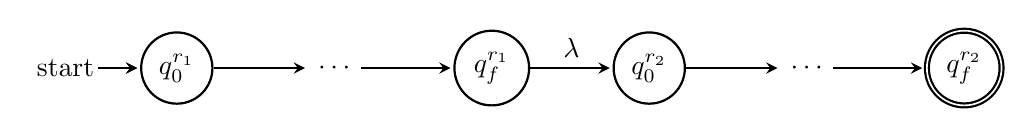
\begin{tikzpicture}[>=stealth, shorten >=1pt, node distance=2.0cm, on grid,
					auto, state/.append style={minimum size=2em}, thick ]
					\node[state,initial]   (A)               {$q_0^{r_1}$};
					\node				   (B)[right of=A]   {$\cdots$};
					\node[state]           (C)[right of=B]   {$q_f^{r_1}$};
					\node[state]   		   (D)[right of=C]   {$q_0^{r_2}$};
					\node				   (E)[right of=D]   {$\cdots$};
					\node[state, accepting](F)[right of=E]   {$q_f^{r_2}$};
					
					
					\path[->] (A) +(-1,0) edge (A)
					
					%Transições:
					%(Partida) edge [tipo da seta] node {simbolo lido} (Destino)
					(A) edge 				            node { }         (B)
					(B) edge 				            node { }         (C)
					(C) edge 				            node {$\lambda$} (D)
					(D) edge 				            node { }         (E)
					(E) edge 				            node { }         (F);
				\end{tikzpicture}
				\caption{$\lambda$-AFN $A^r$ para uma expressão $r_1r_2$.}
				\label{Ima:Automato-F}
			\end{figure}
			
			Agora note que para todo $w \in \Sigma^*$ tal que $w = xy$ com $x, y \in \Sigma^*$ tem-se que,
			\begin{eqnarray*}
				w \in \mathcal{L}(r)  & \Longleftrightarrow & w \in \mathcal{L}(r_1r_2)\\
				& \Longleftrightarrow & xy \in \mathcal{L}(r_1r_2)\\
				& \Longleftrightarrow & xy \in \mathcal{L}(r_1)\mathcal{L}(r_2)\\
				& \Longleftrightarrow & x \in \mathcal{L}(r_1) \text{ e } y \in \mathcal{L}(r_2)\\
				& \Longleftrightarrow & \widehat{\underline{\delta_N}^{r_1}}(q_0^{r_1}, x) \cap \{q_f^{r_1}\} \neq \emptyset \text{ e } \widehat{\underline{\delta_N}^{r_2}}(q_0^{r_2}, y) \cap \{q_f^{r_2}\} \neq \emptyset\\
				& \Longleftrightarrow & \widehat{\underline{\delta_N}}(q_0^{r_1}, x) \cap \{q_f^{r_1}\} \neq \emptyset \text{ e } \widehat{\underline{\delta_N}}(q_0^{r_2}, y) \cap \{q_f^{r_2}\} \neq \emptyset\\
				& \Longleftrightarrow & \widehat{\underline{\delta_N}}(\widehat{\underline{\delta_N}}(q_0^{r_1}, x), y) \cap \{q_f^{r_2}\} \neq \emptyset\\
				& \Longleftrightarrow & \widehat{\underline{\delta_N}}(q_0^{r_1}, xy) \cap \{q_f^{r_2}\} \neq \emptyset\\
				& \Longleftrightarrow & w \in \mathcal{L}(A^r)
			\end{eqnarray*}
			
			\item[\textbf{3º}] \textbf{Caso}: $r = r_1^*$, onde $r_1$ tem exatamente $n$ operadores sendo que $n \geq 0$, assim por \textbf{(HI)} tem-se que existem $A^{r_1} = \langle Q_{r_1}, \Sigma, \underline{\delta_N}^{r_1}, q_0^{r_1}, \{q_f^{r_1}\}\rangle$ tal que $\mathcal{L}(r_1) = \mathcal{L}(A^{r_1})$, agora pode-se criar um novo $\lambda$-AFN $A^r = \langle Q_{r_1} \cup \{q_0, q_{f}\}, \Sigma, \underline{\delta_N}^r, q_0^{r_1}, \{q_{f}\}\rangle$ onde,
			\begin{eqnarray*}
				\underline{\delta_N}^r(q, a) & = & \left\{
				\begin{array}{ll}	
					\underline{\delta_N}^{r_1}(q, a), & \hbox{se } q \in Q_{r_1} - \{q^{r_1}_f\}\\
					\underline{\delta_N}^{r_1}(q, a), & \hbox{se } q  = q^{r_1}_f, a \in \Sigma \\
					\underline{\delta_N}^{r_1}(q, a) \cup \{q_f\}, & \hbox{se } q  = q^{r_1}_f, a = \lambda \\
					\{q_0^{r_1}, q_f\}, & \hbox{se } q = q_0, a = \lambda\\
					\{q_0^{r_1}\}, & \hbox{se } q = q_f, a = \lambda\\
					\emptyset, & \hbox{qualquer outro caso}
				\end{array}\right.
			\end{eqnarray*}
			E para fins de representação tal $\lambda$-AFN $A^r$ tem sua forma como descrita pela figura a seguir.
			\newpage
			\begin{figure}[h]
				\centering
				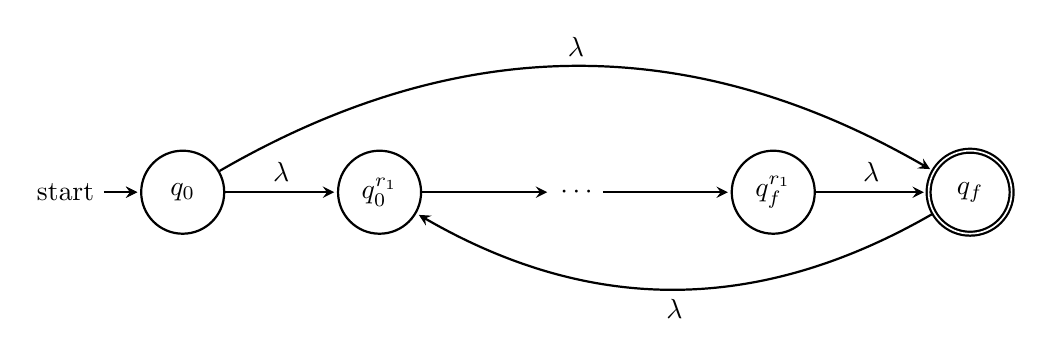
\begin{tikzpicture}[>=stealth, shorten >=1pt, node distance=2.5cm, on grid,
					auto, state/.append style={minimum size=3em}, thick ]
					\node[state,initial]   (A)               {$q_0$};
					\node[state] 		   (B)[right of=A]   {$q_0^{r_1}$};
					\node		           (C)[right of=B]   {$\cdots$};
					\node[state]   		   (D)[right of=C]   {$q_f^{r_1}$};
					\node[state, accepting](E)[right of=D]   {$q_f$};
					
					
					\path[->] (A) +(-1,0) edge (A)
					
					%Transições:
					%(Partida) edge [tipo da seta] node {simbolo lido} (Destino)
					(A) edge 				            node {$\lambda$} (B)
					(A) edge [bend left]				node {$\lambda$} (E)
					(B) edge 				            node { }         (C)
					(C) edge 				            node {} 		 (D)
					(D) edge 				            node {$\lambda$} (E)
					(E) edge [bend left]				node {$\lambda$} (B);
				\end{tikzpicture}
				\caption{$\lambda$-AFN $A^r$ para uma expressão $r_1^*$.}
				\label{Ima:Automato-G}
			\end{figure}
			
			A prova de que $\mathcal{L}(r) = \mathcal{L}(A^r)$ ficará de exercício ao leitor. Agora os três caso anteriores permite afirma que sempre existe um $\lambda$-AFN $A$ tal que $L = \mathcal{L}(A)$.
		\end{itemize}
	\end{itemize}
\end{proof}

Uma consequência imediata deste teorema é apresentada a seguir.

\begin{corollary}
	A linguagem (ou valoração) de qualquer $r \in Exp_\Sigma$ é uma linguagem regular.
\end{corollary}

\begin{proof}
	Direto do Teorema \ref{teo:Exp-AFN} e o Corolário \ref{col:RegularLAFN}.
\end{proof}

\begin{example}\label{exe:Expressao-AFN}
	Dado o alfabeto $\{a,b\}$ e $(ab)^* \in Exp_\Sigma$  pelo Teorema \ref{teo:Exp-AFN} são construídos os autômatos a seguir,
	
	\begin{figure}[h]
		\centering
		\subfloat[$\lambda$-AFN para $\mathcal{L}(a)$.]{
			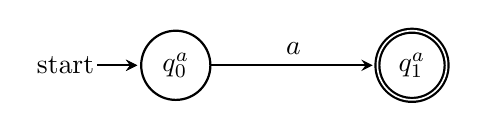
\begin{tikzpicture}[>=stealth, shorten >=1pt, node distance=3cm, on grid,
				auto, state/.append style={minimum size=2.5em}, thick ]
				\node[state,initial]    (A)               {$q^a_0$};
				\node[state, accepting] (B)[right of=A]   {$q^a_1$};
				
				
				\path[->] (A) +(-1,0) edge (A)
				
				%Transições:
				%(Partida) edge [tipo da seta] node {simbolo lido} (Destino)
				(A) edge 				            node {$a$}           (B);
			\end{tikzpicture}
			\label{Ima:Exp-LAFN1}
		}\hfill
		\subfloat[$\lambda$-AFN para $\mathcal{L}(b)$.]{
			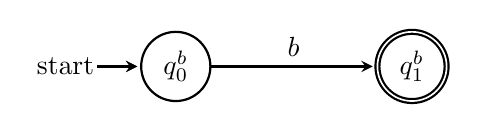
\begin{tikzpicture}[>=stealth, shorten >=1pt, node distance=3cm, on grid,
				auto, state/.append style={minimum size=2.5em}, thick ]
				\node[state,initial]    (A)               {$q^b_0$};
				\node[state, accepting] (B)[right of=A]   {$q^b_1$};
				
				
				\path[->] (A) +(-1,0) edge (A)
				
				%Transições:
				%(Partida) edge [tipo da seta] node {simbolo lido} (Destino)
				(A) edge 				            node {$b$}           (B);
			\end{tikzpicture}
			\label{Ima:Exp-LAFN2}
		}%
		\caption{Os $\lambda$-AFN básicos para as expressões regulares primitivas $a$ e $b$.}
		\label{fig:LAFD-basicos1}
	\end{figure}
	
	Pode-se então gerar o $\lambda$-AFN para reconhecer a concatenação $ab$, tal autômato será gerada pela combinação dos autômatos das Figuras \ref{Ima:Exp-LAFN1} e \ref{Ima:Exp-LAFN2}, gerando com resultado o autômato a seguir como se segue,
	
	\begin{figure}[h]
		\centering
		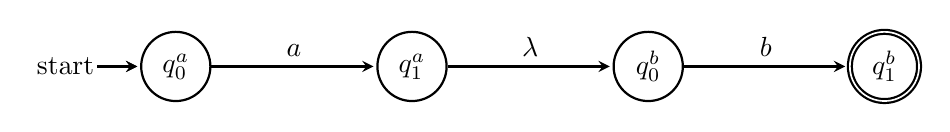
\begin{tikzpicture}[>=stealth, shorten >=1pt, node distance=3cm, on grid,
			auto, state/.append style={minimum size=2.5em}, thick ]
			\node[state,initial]    (A)               {$q^a_0$};
			\node[state] 			(B)[right of=A]   {$q^a_1$};
			\node[state] 			(C)[right of=B]   {$q^b_0$};
			\node[state, accepting] (D)[right of=C]   {$q^b_1$};
			
			
			\path[->] (A) +(-1,0) edge (A)
			
			%Transições:
			%(Partida) edge [tipo da seta] node {simbolo lido} (Destino)
			(A) edge 				            node {$a$}           (B)
			(B) edge 				            node {$\lambda$}     (C)
			(C) edge 				            node {$b$}           (D);
		\end{tikzpicture}
		\caption{$\lambda$-AFN para as expressões regular $\mathcal{L}(ab)$.}
		\label{fig:LAFD-basicos2}
	\end{figure}
	
	Para finalizar é necessário agora apresentar o autômato que reconheça o fecho de Kleene da expressão $ab$, tal autômato é construído seguindo o Teorema \ref{teo:Exp-AFN}, e tal autômato é representado pelo grafo de transição esboçado na Figura \ref{fig:LAFD-basicos3} a seguir.
	
	\begin{figure}[h]
		\centering
		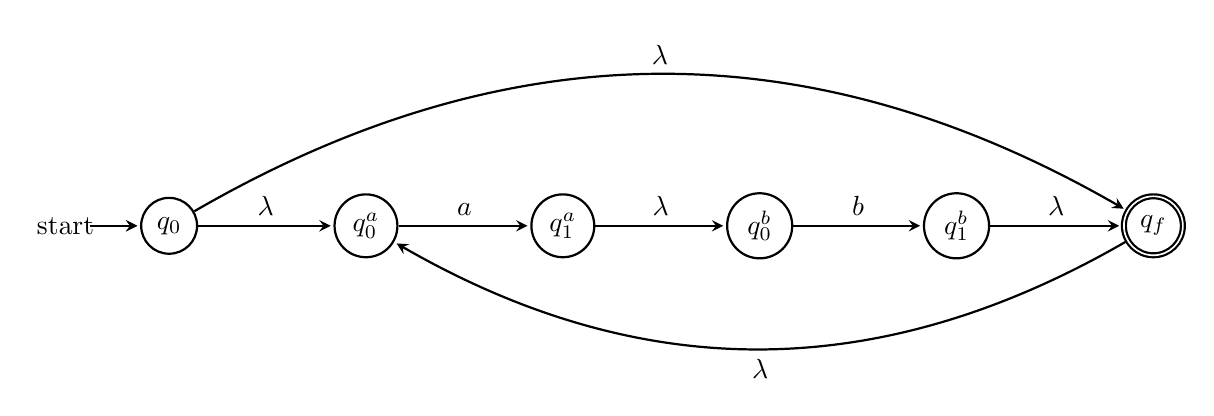
\begin{tikzpicture}[>=stealth, shorten >=1pt, node distance=2.5cm, on grid,
			auto, state/.append style={minimum size=2.0em}, thick ]
			\node[state,initial]    (A)               {$q_0$};
			\node[state]		    (B)[right of=A]   {$q^a_0$};
			\node[state] 			(C)[right of=B]   {$q^a_1$};
			\node[state] 			(D)[right of=C]   {$q^b_0$};
			\node[state]			(E)[right of=D]   {$q^b_1$};
			\node[state, accepting] (F)[right of=E]   {$q_f$};
			
			
			\path[->] (A) +(-1,0) edge (A)
			
			%Transições:
			%(Partida) edge [tipo da seta] node {simbolo lido} (Destino)
			(A) edge 				            node {$\lambda$}     (B)
			(B) edge 				            node {$a$}           (C)
			(C) edge 				            node {$\lambda$}     (D)
			(D) edge 				            node {$b$}           (E)
			(E) edge 				            node {$\lambda$}     (F)
			(A) edge [bend left]	            node {$\lambda$}     (F)
			(F) edge [bend left]	            node {$\lambda$}     (B);
		\end{tikzpicture}
		\caption{$\lambda$-AFN para as expressões regular $\mathcal{L}((ab)^*)$.}
		\label{fig:LAFD-basicos3}
	\end{figure} 
\end{example}

\newpage
\begin{remark}
	Apenas na demonstração a seguir considere que o símbolo $\Sigma$ representa o somatório enumerável, com respeito a soma $(+)$ das expressões regulares, além disso, para fins de representação durante tal prova a letra $X$ irá representar um alfabeto genérico qualquer.
\end{remark}

\begin{theorem}
	Se $L$ é uma linguagem regular, então existe uma expressão regular $r$ tal que $L = \mathcal{L}(r)$.
\end{theorem}

\begin{proof}
	Sem perda de generalidade suponha que $L = \mathcal{L}(A)$ para algum $\lambda$-AFN $A = \langle \{q_1, \cdots, q_n\}, X, \delta, q_1, F \rangle$ em que $n \geq 1$. Agora será construído para todo $k \leq n$ a expressão regular $r^k_{i,j}$ é definida recursivamente como sendo:
	\begin{eqnarray*}
		r^0_{i,j} & = &  \left\{
		\begin{array}{ll}	
			\displaystyle\sum_{\delta(q_i, a, q_j)} a, & \hbox{se } i \neq j\\
			\displaystyle\lambda + \sum_{\delta(q_i, a, q_j)} a, & \hbox{se } i = j\\
		\end{array}\right.\\
		r^{k}_{i,j} & = & (r^{k-1}_{i,k}(r^{k-1}_{k,k})^* r^{k-1}_{k,j}) + r^{k-1}_{i,j}
	\end{eqnarray*}
	note que $r^{k}_{i,j}$ é a expressão regular cuja valoração é o conjunto de todas as palavras $w \in X^*$ tal que $\widehat{\delta}(q_i, w) = q_j$ de forma que nenhum estado intermediário $q_p$ com $p > k$ seja usado na computação (para detalhes deste fato consulte \cite{benjaLivro2010, hopcroft2008}). Agora uma vez que $A$ pode ter vários estados $q_f \in F$ tem-se então que cada $w \in X^*$ tal que $\widehat{\delta}(q_1, w) = q_f$ é uma palavra aceita por $A$, ou seja, $w \in \mathcal{L}(A)$ e, portanto, para $n = \# Q$ a valoração da expressão regular $r$ definida por, 
	\begin{eqnarray*}
		r = \sum_{q_f \in F} r^n_{1, f}
	\end{eqnarray*}
	é exatamente o conjunto de todas as palavras aceitas por $A$, ou seja, $\mathcal{L}(A) = \mathcal{L}(r)$. 
\end{proof}

\begin{example}
	Considere o AFD esboçado pela Figura \ref{fig:AFD-Expressao}, 
	
	\begin{figure}[h]
		\centering
		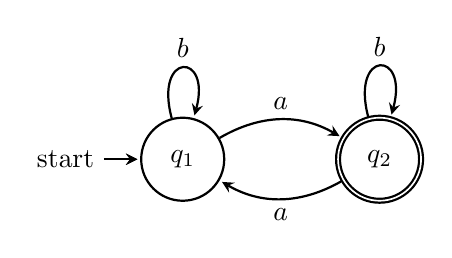
\begin{tikzpicture}[>=stealth, shorten >=1pt, node distance=2.5cm, on grid,
			auto, state/.append style={minimum size=3.0em}, thick ]
			\node[state,initial]    (A)               {$q_1$};
			\node[state, accepting] (B)[right of=A]   {$q_2$};
			
			
			\path[->] (A) +(-1,0) edge (A)
			
			%Transições:
			%(Partida) edge [tipo da seta] node {simbolo lido} (Destino)
			(A) edge [loop above]				node {$b$}     ( )
			(B) edge [loop above]				node {$b$}     ( )
			(A) edge [bend left]	            node {$a$}     (B)
			(B) edge [bend left]	            node {$a$}     (A);
		\end{tikzpicture}
		\caption{Um AFD que computa sobre o alfabeto $\{a, b\}$.}
		\label{fig:AFD-Expressao}
	\end{figure} 
	
	Como $n = \# Q$ tem-se que $n = 2$, e portanto, a expressão regular cuja valoração corresponde a linguagem do AFD será dada por, 
	\begin{eqnarray}\label{eq:AFD-EXP0}
		r^2_{1, 2} & = & (r^{1}_{1, 2}(r^{1}_{2, 2})^*r^{1}_{2, 2}) + r^{1}_{1, 2}
	\end{eqnarray}
	Note porém que, 
	\begin{eqnarray}\label{eq:AFD-EXP1}
		r^{1}_{1, 2}  & = & (r^{0}_{1, 1}(r^0_{1,1})^* r^0_{1,2}) + r^0_{1,2} \nonumber \\
		& \equiv & ((\lambda + b)(\lambda + b)^* a) + a\\
		& \equiv & b^*a \nonumber
	\end{eqnarray}
	e
	\begin{eqnarray}\label{eq:AFD-EXP2}
		r^{1}_{2, 2}  & = & (r^{0}_{2, 1}(r^0_{1,1})^* r^0_{1,2}) + r^0_{2,2} \nonumber \\
		& \equiv & (a(\lambda + b)^* a) + (\lambda + b)\\
		& \equiv & ab^* a + \lambda + b \nonumber
	\end{eqnarray}
	substituindo as Equações (\ref{eq:AFD-EXP1}) e (\ref{eq:AFD-EXP2}) na Equação (\ref{eq:AFD-EXP0}) tem-se que,
	\begin{eqnarray*}
		r^2_{1, 2} & = & (b^*a(ab^* a + \lambda + b)^* ab^* a + \lambda + b) + (b^*a)\\
		& \equiv & b^*a(ab^*a + b)^*(ab^* a + \lambda) + b^*a\\
		& \equiv & b^*a(ab^*a + b)^*+ b^*a\\
		& \equiv & b^*a(ab^*a + b)^*
	\end{eqnarray*}
\end{example}

\section{Gramática Regulares}\label{sec:GramaticaRegular}

Nas seções anteriores foram apresentados dois formalismos para as linguagens regulares, a saber, formalismo operacional (os autômatos) e o formalismo denotacional (as expressões regulares). Nesta seção será apresentado um terceiro formalismo para as linguagens regulares, sendo este um formalismo gerador (ou axiomático) \cite{menezes1998LFA}. 

\begin{definition}[Gramática Linear]\label{def:GramaticaLinear}
	Uma gramática formal $G = \langle V, \Sigma, S, P \rangle$ e dita Linear à Direta, ou simplesmente GLD, se todas as suas produções são da forma, 
	$$A \rhd wB$$
	e é dita Linear à Esquerda, ou simplesmente GLE, se todas as suas produções são da forma, 
	$$A \rhd Bw$$
	onde $A \in V, B \in V \cup \{\lambda\}$ e $w \in \Sigma^*$.
\end{definition}

\begin{example}
	A gramática $G_1 = \langle \{B, S , A\}, \{a, b\}, S, P \rangle$ onde $P$ é formado pelas regras:
	\begin{eqnarray*}
		S & \rhd & aaB\\
		B & \rhd & bb
	\end{eqnarray*}
	é uma GLD.
\end{example}

\begin{example}\label{exe:GLE1}
	A gramática $G_1 = \langle \{X, S , Y\}, \{0, 1\}, S, P \rangle$ onde $P$ é formado pelas regras:
	\begin{eqnarray*}
		S & \rhd & X001\\
		S & \rhd & Y011\\
		X & \rhd & S01\\
		Y & \rhd & \lambda
	\end{eqnarray*}
	é uma GLE.
\end{example}

Em uma gramática formal $G$ quando para uma palavra $w$ existem $w_1, \cdots, w_n$ tal que há as seguintes regras $w \rhd w_1, \cdots, w \rhd w_n \in P$, é comum para simplificar a escrita do conjunto de regras usar a notação $w \rhd w_1 \mid \cdots \mid w_n$. 

\begin{example}\label{exe:GLE}
	Considere a GLE apresentada no Exemplo \ref{exe:GLE1} o conjunto $P$ da mesma poderia ser escrito como:
	\begin{eqnarray*}
		S & \rhd & X001 \mid Y011\\
		X & \rhd & S01\\
		Y & \rhd & \lambda
	\end{eqnarray*}
\end{example}

\begin{definition}[Gramática Regular]
	Uma gramática formal $G$ é dita regular sempre que ela for linear à esquerda ou à direita.
\end{definition}

Um tipo mais rigoroso de gramática regular como comentado em \cite{benjaLivro2010, linz2006},  são as chamadas gramática regulares unitárias definidas a seguir.

\begin{definition}[Gramáticas Regulares Unitárias]
	Uma gramática regular $G$ é dita unitária à esquerda (à direita) se ela é linear à esquerda (à direita) e toda produção é da forma $A \rhd Bw$ $(A \rhd wB)$ com $A \in V, B \in V \cup \{\lambda\}$ e $w \in \Sigma \cup \{\lambda\}$.
\end{definition}

\begin{example}
	A gramática $G$ do Exemplo \ref{exe:GLE} é uma gramática regular pois é uma GLE, porém não é uma gramática regular unitária.
\end{example}

\begin{remark}
	De forma natural como o leitor deve estar pensando agora,  duas gramática $G_1$ e $G_2$ serão ditas equivalentes sempre que elas gerarem a mesma linguagens.
\end{remark}

O próximo resultado estabelece que gramática regulares e gramática regulares unitárias tem o mesmo poder de geração de linguagens.

\begin{theorem}\label{teo:SimplificacaoRegular}
	$L = \mathcal{L}(G)$ para alguma gramática regular $G$ se, e somente se, existe uma gramática regular unitária $G'$ na mesma direção (esquerda ou direita) tal que $L = \mathcal{L}(G')$.
\end{theorem}

\begin{proof}
	$(\Rightarrow)$ Suponha que $L = \mathcal{L}(G)$ para alguma gramática regular $G = \langle V, \Sigma, S, P \rangle$ tal que $G$ seja linear à esquerda (a prova é similar para o caso à direita). Agora construa uma nova gramática $G' = \langle V', \Sigma, S, P' \rangle$ tal que $P'$ é definido usando as seguintes regras: 
	
	\begin{itemize}
		\item[R1:] Se $A \rhd Bw \in P$ onde $B \in V \cup \{\lambda\},  |w| \leq 1$, então $A \rhd Bw \in P'$.
		\item[R2:] Se $A \rhd Ca_1\cdots a_n \in P$ onde $B \in V$ e $a_i \in \Sigma$ sendo $1 \leq i \leq n$ e $n > 1$, então tem-se que $A \rhd B_na_n, B_n \rhd B_{n-1}a_{n-1}, \cdots, B_2 \rhd Ca_1 \in P'$.
		\item[R3:] Se $A \rhd a_1\cdots a_n \in P$ onde $a_i \in \Sigma$ sendo $1 \leq i \leq n$ e $n \geq 2$, então tem-se que $A \rhd B_na_n, B_n \rhd B_{n-1}a_{n-1}, \cdots, B_2 \rhd B_1a_1, B_1 \rhd \lambda \in P'$.
	\end{itemize}
	
	Para as regras R2 e R3 todo $B_i$ é uma nova variável existente em $V'$ que não existe originalmente em $V$. Claramente a gramática $G'$ é regular unitária à esquerda. Também não é difícil mostra por indução sobre o tamanho das derivações que para todo $w \in \Sigma^*$ tem-se que $S \gg^*_G w$ se, e somente se, $S \gg^*_{G'} w$, portanto, $\mathcal{L}(G) = \mathcal{L}(G')$.
	
	$(\Leftarrow)$ Trivial uma vez que toda gramática regular unitária à esquerda (à direita) é um caso particular de gramática regular à esquerda (à direita).
\end{proof}

\begin{example}\label{exe:GRU}
	Considerando a gramática regular do Exemplo \ref{exe:GLE} usando o Teorema \ref{teo:SimplificacaoRegular} é gerado a gramática regular unitária $G' = \langle \{S, B_3, B_2, C_3, C_2, X, D_2, Y\}, \{0, 1\}, S, P'\rangle$ onde $P'$ é formado pelas regras:
	\begin{eqnarray*}
		S & \rhd & B_31 \mid C_31\\
		B_3 & \rhd & B_20\\
		B_2 & \rhd & X0\\
		C_3 & \rhd & C_21\\
		C_2 & \rhd & Y0\\
		X & \rhd & D_21\\
		D_2 & \rhd& S0\\
		Y & \rhd & \lambda
	\end{eqnarray*}
\end{example}

\begin{remark}
	Obviamente a gramática do Exemplo \ref{exe:GRU} poderia ser otimizada para usar menos variáveis, porém otimização não é o foco de interesse no Teorema \ref{teo:SimplificacaoRegular}.
\end{remark} 

O próximo resultado estabelece o poder de geração das gramáticas regulares à direta.

\begin{theorem}\label{teo:GRD-AFD}
	$L = \mathcal{L}(G)$ para alguma gramática regular à direta $G$ se, e somente se, $L$ é uma linguagem regular.
\end{theorem}

\begin{proof}
	$(\Rightarrow)$ Suponha que $L = \mathcal{L}(G)$ para alguma gramática regular à direta $G$, assim pelo Teorema \ref{teo:SimplificacaoRegular} existe uma gramática regular unitária à direita $G' = \langle V, \Sigma, S, P \rangle$ tal que $L = \mathcal{L}(G')$, sem perda de generalidade\footnote{Basta gerar uma nova gramática onde toda regra da forma $A \rhd a$ com $a \in \Sigma$ foi substituída pelas regras $A \rhd aC$ e $C \rhd \lambda$ onde $C$ é uma variável nova criada, obviamente a nova gramática continua equivalentes a antiga.} pode-se assumir que toda regra em $P$ é da forma $A \rhd aB$ ou $A \rhd \lambda$ com $A, B \in V$ e $a \in \Sigma \cup \{\lambda\}$, dito isto, pode-se agora construir um $\lambda$-AFN $M = \langle V \cup \{q_f\}, \Sigma, \underline{\delta_N}, S, \{q_f\} \rangle$ tal que:
	\begin{eqnarray*}
		B \in \underline{\delta_N}(A, a) & \Longleftrightarrow & A \rhd aB \in P\\
		q_f \in \underline{\delta_N}(A, \lambda)& \Longleftrightarrow & A \rhd \lambda \in P
	\end{eqnarray*}
	Agora será mostrado por indução sobre o tamanho das derivações em $G'$ que se $w$ é derivada por $G'$ e $w \in \Sigma^*$, então é aceita por $M$.
	\begin{itemize}
		\item \textbf{Base da indução}:
		
		Quando $w$ é derivada em $G'$ com uma única derivação tem-se então duas situações possíveis:
		\begin{itemize}
			\item[(1)] Quando $w = \lambda$, obrigatoriamente existe uma regra da forma $S \rhd \lambda$, e pela construção de $M$ tem-se que $q_f \in \underline{\delta_N}(S, \lambda)$, logo $\widehat{\underline{\delta_N}}(S, \lambda) \cap \{q_f\} \neq \emptyset$ e, portanto, $\lambda \in L(M)$. 
			\item[(2)] Quando $w = aB$, existe em $P$ uma regra da forma $S \rhd aB$ com $a \in \Sigma \cup \{\lambda\}$ e $B \in V$, assim pela construção de $M$ tem-se que $B \in \underline{\delta_N}(A, a)$. Como $aB \notin \Sigma^*$ não há mais nada a fazer nesse caso.
		\end{itemize}
		
		
		\item \textbf{Hipótese indutiva (HI)}:
		
		Suponha que $S \gg^*_{G'} w$ em $n$ derivação com $n \geq 1$ tal que:
		\begin{itemize}
			\item[(1)] Se $w \in \Sigma^*$, então $w \in \mathcal{L}(M)$.
			\item[(2)] Se $w = a_1\cdots a_{n-1}B$ com $a_i \in \Sigma \cup \{\lambda\}$ para todo $1 \leq i \leq n-1$ e $B \in V$, então $B \in \widehat{\underline{\delta_N}}(S, a_1\cdots a_{n-1})$.
		\end{itemize}
		
		\item \textbf{Passo indutivo}:
		
		Agora dado que $S \gg^*_{G'} w'$ em $n+1$ derivações, tem-se obrigatoriamente que acontece o caso (2) de \textbf{(HI)} e nesse caso duas situações são possíveis:
		\begin{itemize}
			\item[(1)] Se $w' \in \Sigma^*$, então $w = a_1\cdots a_{n-1}B$ com $a_i \in \Sigma \cup \{\lambda\}$ para todo $1 \leq i \leq n-1$ e existe em $P$ uma produção $B \rightarrow \lambda$, e assim, $w' = a_1\cdots a_{n-1}$, nesta situação pelo caso (2) de \textbf{(HI)} tem-se que $B \in \widehat{\underline{\delta_N}}(S, a_1\cdots a_{n-1})$ e como $B \rightarrow \lambda$ pelo construção de $M$ tem-se que $q_f \in \underline{\delta_N}(B, \lambda)$, consequentemente, $\widehat{\underline{\delta_N}}(S, a_1\cdots a_{n-1}) \cap \{q_f\} \neq \emptyset$ e, portanto, $w' \in \mathcal{L}(M)$.
			\item[(2)] Se $w' = a_1\cdots a_{n-1}B$ com $a_i \in \Sigma \cup \{\lambda\}$ para todo $1 \leq i \leq n-1$ e $B \in V$, então pela construção de $M$ tem-se que $B \in \widehat{\underline{\delta_N}}(S, w)$ como $w' \notin \Sigma^*$ não há mais nada a fazer nesse caso.
		\end{itemize}
	\end{itemize}
	Portanto, o raciocínio indutivo anterior garante que sempre que  $w$ é derivada por $G'$ e $w \in \Sigma^*$ tem-se que $w \in \mathcal{L}(M)$ e assim pode-se afirmar pelo Corolário \ref{col:RegularLAFN} que $L$ é regular. $(\Leftarrow)$ Suponha que $L$ é uma linguagem regular assim por definição existe um AFD $M = \langle Q, \Sigma, \delta, q_0, F \rangle$ tal que $L = \mathcal{L}(M)$, assim construa uma gramática regular unitária à direita $G = \langle Q, \Sigma, q_0, P \rangle$ onde o conjunto $P$ é definido usando as regras a seguir, 
	\begin{itemize}
		\item[(a)] Se $\delta(q_i, a) = q_j$, então $q_i \rhd aq_j \in P$.
		\item[(b)] Se $q_i \in F$, então $q_i \rhd \lambda \in P$.
	\end{itemize} 
	Agora note que para todo $w \in \Sigma^*$ com $w = a_1 \cdots a_n$ tem-se que, 
	\begin{eqnarray*}
		w \in \mathcal{L}(M) & \Longleftrightarrow & \widehat{\delta}(q_0, w) \in F\\
		& \Longleftrightarrow & \widehat{\delta}(q_0, a_1 \cdots a_n) \in F\\
		& \Longleftrightarrow & (\exists q_f \in F)[\widehat{\delta}(q_0, w) = q_f]\\
		& \Longleftrightarrow & (\exists q_1, \cdots, q_{n-1} \in Q,  q_f \in F)[\delta(q_0, a_1) = q_1 \land \cdots \land \delta(q_{n-1}, a_n) = q_f]\\
		& \Longleftrightarrow & (\exists q_1, \cdots, q_{n-1} \in Q,  q_f \in F)[q_0 \rhd a_1q_1, \cdots, q_{n-1} \rhd a_nq_f, q_f \rhd \lambda \in P]\\
		& \Longleftrightarrow & q_0 \gg^* a_1 \cdots a_n\\
		& \Longleftrightarrow & q_0 \gg^* w\\
		& \Longleftrightarrow & w \in \mathcal{L}(G)
	\end{eqnarray*} 
	portanto, $\mathcal{L}(M) = \mathcal{L}(G)$ o que conclui a prova.
\end{proof}

\begin{lemma}\label{lema:GRD-Reversa}
	Se $L$ é gerada por uma gramática à direita, então $L^r$ é gerada por uma gramática regular à direita.
\end{lemma}

\begin{proof}
	Suponha que $L$ é gerada por uma gramática à direita $G$, ou seja, $L = \mathcal{L}(G)$, assim pelo Teorema \ref{teo:GRD-AFD} tem-se que $L$ é regular, logo existe um AFD $M = \langle Q, \Sigma, \delta, q_0, F\rangle$ tal que $L = \mathcal{L}(M)$, agora construa um $\lambda$-AFN $M_1 = \langle Q \cup \{q_f\}, \Sigma, \underline{\delta_N}, q_0, \{q_f\}\rangle$ tal que,
	\begin{eqnarray*}
		\underline{\delta_N}(q, a) & = & \left\{\begin{array}{ll}	
			\{\delta(q, a)\}, & \hbox{se } q \in Q, a \in \Sigma\\
			\{q_f\}, & \hbox{se } q \in F, a = \lambda \\
			\emptyset, & \hbox{qualquer outro caso}
		\end{array}\right.
	\end{eqnarray*}
	claramente $L = \mathcal{L}(M_1)$, agora construa um novo $\lambda$-AFN $M_2 = \langle Q \cup \{q_f\}, \Sigma, \underline{\delta'_N}, q_f, \{q_0\}\rangle$ onde para todo $q \in Q \cup \{q_f\}$ e $a \in \Sigma \cup \{\lambda\}$ tem-se que,
	\begin{eqnarray*}
		q_i \in \underline{\delta'_N}(q_j, a) & \Longleftrightarrow & q_j \in \underline{\delta_N}(q_i, a)
	\end{eqnarray*}
	pela construção de $M_2$ é claro que  $w \in \mathcal{L}(M_1) \Longleftrightarrow w^r \in \mathcal{L}(M_2)$ e, portanto, $L^r = \mathcal{L}(M_2)$. Desde que $M_2$ é um $\lambda$-AFN pelo Corolário \ref{col:RegularLAFN} tem-se que $L^r$ é uma linguagem regular, consequentemente, pelo Teorema \ref{teo:GRD-AFD} existe uma gramática regular à direita $G'$ tal que $L = \mathcal{L}(G')$, o que conclui a prova.
\end{proof}

O próximo resultado mostra que gramática regulares à esquerda e à direita são equivalentes.

\begin{theorem}[Mudança de direção regular]\label{teo:MudacaDeLadoGramatica}
	$L$ é gerada por uma gramática à esquerda se, e somente se, $L$ é gerada por uma gramática regular à direita.
\end{theorem}

\begin{proof}
	$(\Rightarrow)$ Suponha que $L$ é gerada por uma gramática à esquerda $G = \langle V, \Sigma, S, P \rangle$, pelo Teorema \ref{teo:SimplificacaoRegular} pode-se assumir que $G$ é uma gramática regular unitária também a esquerda, assim todas as regras em $P$ são da forma $A \rhd Ba$ com $A \in V, B \in V \cup \{\lambda\}$ e $a \in \Sigma \cup \{\lambda\}$. Sem perda de generalidade\footnote{Basta gerar uma nova gramática onde toda regra da forma $A \rhd a$ com $a \in \Sigma$ foi substituída pelas regras $A \rhd Ca$ e $C \rhd \lambda$ onde $C$ é uma variável nova criada.} pode-se construir uma nova gramática regular unitária à esquerda $G' = \langle V', \Sigma, S, P'\rangle$ onde toda regra em $P'$ é da forma $A \rhd Ba$ ou $A \rhd \lambda$ com $A, B \in V'$ e $a \in \Sigma \cup \{\lambda\}$ claramente pela construção de $G'$ tem-se que $\mathcal{L}(G) = \mathcal{L}(G')$, agora construa um $\lambda$-AFN $M = \langle V' \cup \{q_f\}, \Sigma, \underline{\delta_N}, S, \{q_f\} \rangle$ onde, 
	\begin{eqnarray*}
		B \in \underline{\delta_N}(A, a) & \Longleftrightarrow & A \rhd Ba \in P\\
		q_f \in \underline{\delta_N}(A, \lambda)& \Longleftrightarrow & A \rhd \lambda \in P
	\end{eqnarray*} 
	Agora note que para todo $w = a_1\cdots a_n \in \Sigma^*$ tem-se que,
	\begin{eqnarray*}
		w \in \mathcal{L}(G') & \Longleftrightarrow &  a_1\cdots a_n \in \mathcal{L}(G')\\
		& \Longleftrightarrow & S \gg_{G'}^* a_1\cdots a_n\\
		& \Longleftrightarrow & (\exists A_1 \cdots A_n, S \in V)\\
		& & [S \rhd A_na_n, A_n \rhd A_{n-1}a_{n-1}, \cdots, A_{2} \rhd A_1a_1, A_1 \rhd \lambda \in P']\\
		& \Longleftrightarrow & (\exists A_1 \cdots A_n, S \in V)\\
		& & [A_n \in \underline{\delta_N}(S, a_n), A_{n-1} \in \underline{\delta_N}(A_n, a_{n-1}), \cdots,  A_{1} \in \underline{\delta_N}(A_2, a_{1}), \\
		& &  q_f \in \underline{\delta_N}(A_1, \lambda)]\\
		& \Longleftrightarrow & a_n\cdots a_1 \in \mathcal{L}(M)\\
		& \Longleftrightarrow & w^r \in \mathcal{L}(M)
	\end{eqnarray*}
	Logo $\mathcal{L}(M) = \mathcal{L}(G')^r$, desde que $M$ é um $\lambda$-AFN tem-se pelo Corolário \ref{col:RegularLAFN} que $\mathcal{L}(G')^r$ é regular, assim pelo Teorema \ref{teo:GRD-AFD} existe uma gramática regular à direita $\hat{G_1}$ que a gera, ou seja, $\mathcal{L}(\hat{G_1}) = \mathcal{L}(G')^r$, mas pelo Lema \ref{lema:GRD-Reversa} irá existir outra gramática regular à direita $\hat{G_2}$ tal que $\mathcal{L}(\hat{G_2}) = \mathcal{L}(\hat{G_1})^r$, mas $ \mathcal{L}(\hat{G_1})^r = (\mathcal{L}(G')^r)^r = (\mathcal{L}(G)^r)^r = (L^r)^r = L$, portanto, $L$ é gerada por uma gramática regular à direita. $(\Leftarrow)$ Suponha que que $L$ é gerada por uma gramática regular à direita, ou seja, que existe uma gramática regular a direita $G$ tal que $L = \mathcal{L}(G)$, assim pelo Lema \ref{lema:GRD-Reversa} irá existir outra gramática regular à direita $G_1 = \langle V, \Sigma, S, P \rangle$ tal que $L^r = \mathcal{L}(G_1)$, sem perda de generalidade pelo Teorema \ref{teo:SimplificacaoRegular} pode-se assumir que $G_1$ é regular unitária à direita, logo todas as suas produções são da forma $A \rhd aB$ com $A \in V, B \in V \cup \{\lambda\}$ e $a \in \Sigma \cup \{\lambda\}$. Dito isso construa uma nova gramática $G_2 = \langle V, \Sigma, S, P'\rangle$ onde $P' = \{A \rhd Ba \mid A \rhd Ba \in P\}$, claramente $G_2$ é unitária à esquerda. Mas pela construção de $G_2$ fica claro que $S \gg_{G_1}^* w \Longleftrightarrow S \gg_{G_2}^* w^r$, logo $\mathcal{L}(G_1)^r = \mathcal{L}(G_2)$, mas desde que, $\mathcal{L}(G_1)^r = (L^r)^r = L$, tem-se então que $L$ é gerada por uma gramática linear à esquerda, o que completa  a prova.
\end{proof}

\begin{example}
	Dado a gramática regular à direita $G_1 = \langle \{A, B, C\}, \{a, b\}, A, P_1 \rangle$ com $P_1$ é formado pelas seguintes regras,
	\begin{eqnarray*}
		A & \rhd & aC \mid B \\
		B & \rhd & bB \mid \lambda\\
		C & \rhd & aA
	\end{eqnarray*}
	claramente $\mathcal{L}(G_1) = \{w \in \{a, b\}^* \mid w = a^{2m}b^n \hbox{ com } m,n \in \mathbb{N}\}$,  agora usando a construção exposta pelo Teorema \ref{teo:MudacaDeLadoGramatica}, é possível construir a gramática regular à esquerda $G_2 = \langle \{A, B, C\}, \{a, b\}, B, P_2 \rangle$ onde $P_2$ é formado pelas seguintes regras,
	\begin{eqnarray*}
		B & \rhd & Bb \mid Ab \mid A\\
		A & \rhd & Ca \mid \lambda\\
		C & \rhd & Aa 
	\end{eqnarray*}
	e obviamente $\mathcal{L}(G_2) = \{w \in \{a, b\}^* \mid w = a^{2m}b^n \hbox{ com } m,n \in \mathbb{N}\}$.
\end{example}

\begin{remark}
	Para esse questionário sempre que $w \in \Sigma^*$ e $c \in \Sigma$ a notação $|w|_c$ irá representar o número de $c$'s que existem na palavra $w$.
\end{remark}

\begin{problemset}
	\item Considere o autômato na Figura \ref{fig:AutomaExercicioLR8} e responda o que é solicitado.
	\begin{figure}[h]
		\centering
		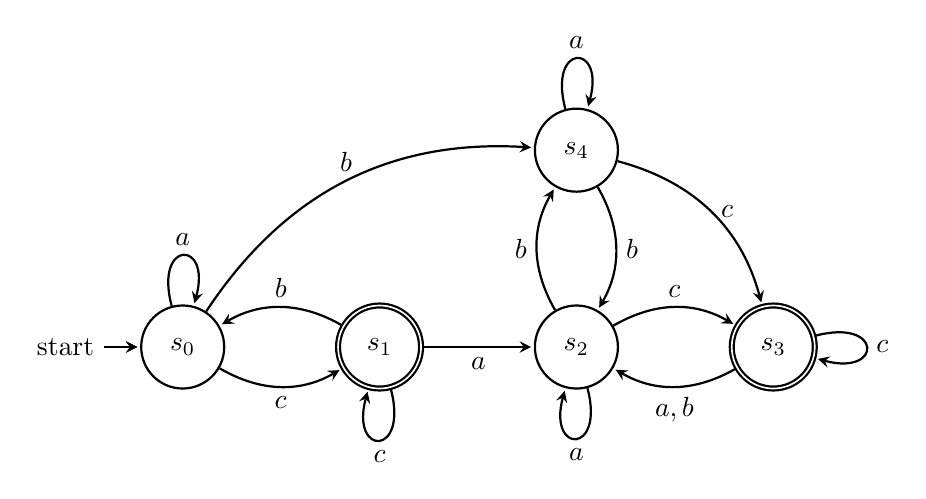
\begin{tikzpicture}[>=stealth, shorten >=1pt, node distance=2.5cm, on grid, auto, state/.append style={minimum size=3em}, thick ]
			\node[state, initial]				(A)               	{$s_0$};
			\node[state, accepting]				(B) [right of=A] 	{$s_1$};
			\node[state]				        (C) [right of=B] 	{$s_2$};
			\node[state, accepting]		        (D) [right of=C] 	{$s_3$};
			\node[state]				        (E) [above of=C] 	{$s_4$};
			\path[->] (A) +(-1,0) edge (A)
			
			%Transições:
			%(Partida) edge [tipo da seta] node {simbolo lido} (Destino)
			(A) edge [bend right]  				node [below] {$c$}		 (B)
			(A) edge [loop above]  				node 		 {$a$}		 ( )
			(A) edge [bend left]  				node [above] {$b$}		 (E)
			(B) edge [bend right]  				node [above] {$b$}		 (A)
			(B) edge  							node [below] {$a$}	 	 (C)
			(B) edge [loop below]  				node 		 {$c$}		 ( )
			(C) edge [bend left]  				node [above] {$c$}	 	 (D)
			(C) edge [bend left]  				node [left]  {$b$}		 (E)
			(C) edge [loop below]  				node 		 {$a$}		 ( )
			(E) edge [bend left]  				node [right] {$b$}		 (C)
			(E) edge [bend left]  				node [right] {$c$}	 	 (D)
			(E) edge [loop above]  				node 		 {$a$}		 ( )
			(D) edge [loop right]  				node 		 {$c$}       ( )
			(D) edge [bend left]  				node [below] {$a,b$} 	 (C);
		\end{tikzpicture}
		\caption{Autômato para o exercício 1.}
		\label{fig:AutomaExercicioLR8}
	\end{figure}

	\begin{enumerate}
		\item Verifique se as palavras: $abccaaabacab, ccccbacabacbb, bbacabb, aaccca, aaabb, acacabb,$ $bbacac$ e $ccabbbacac$ são aceitas ou não pelo autômato.
		\item $\lambda$ é aceito por este autômato?
		\item Traduza o grafo de transição para a notação algébrica.
	\end{enumerate}

	\item Construa um AFD que compute cada linguagem a seguir.
	\begin{enumerate}
		\item $L_1 = \{\lambda, 00101111, 11001101, 1\}$.
		\item $L_2 = \{w10 \in \{0,1\}^* \mid w = (001)^n11 \text{ com } n \in \mathbb{N}\}$.
		\item $L_3 = \{w \in \{a,b\}^* \mid w = a^{2m}b^{2n+1} \text{ ou } w = aab^{3m + 3}b^n \text{ com } m,n \in \mathbb{N}\}$.
		\item $L_4 = \{w \in \{a,b,c,d\}^* \mid w \text{ não contém as subcadeias } ab \text{ e } cd\}$.
		\item $L_5 = \{w \in \{0,1\}^* \mid (\forall n \in \mathbb{N})[|w|_1 \neq 3n]\}$.
		\item $L_6 = \{w \in \{0,1\}^* \mid w = x_1\cdots x_n \text{ e } x_i = 0 \text{ se } i \text{ for par, senão } x_i = 1 \text{, sendo } n \in \mathbb{N}\}$.
		\item $L_7 = \{w \in \{x, y, z\}^* \mid \text{Se } w \text{ contém a sub-palavra } zz \text{, então à  direita da sub-palavra }$ $zz \text{ não ocorre a sub-palavra } yy \}$.
		\item $L_8 = \{aaa, aab, aba, abb, baa, bab, bba, bbb\} \cup \{bbca, ccab, ccab, baba\}$.
		\item $L_9 = \{uv \in \{0,1\}^* \mid u = 1^m0111, v = 0100^p1 \text{ com } m, p \in \mathbb{N}\}$.
		\item $L_{10} = \{w \in \{0,1\}^* \mid w \text{ é um número binário multiplo de  } 3\}$.
	\end{enumerate}

	\item Considerando o alfabeto $\Sigma = \{c, d\}$ para cada uma das linguagens definidas pelas propriedades a seguir construa um AFD que a compute.
	\begin{enumerate}
		\item $w$ possui exatamente um único símbolo $d$, e este não aparece no final das palavras.
		\item $w$ tem apenas uma única sub-palavra $dd$.
		\item $w$ não contém três $d$'s seguidos.
		\item $w$ possui pelo menos um $c$.
		\item $w$ possui 6 ou menos símbolos, e não existe as sub-palavras $cc$ e $dd$.
		\item $w$ tem mais que $4$ símbolos $c$.
		\item $w$ é da forma $db^4wb^5d$ com $w \in \Sigma^*$.
		\item $w$ possui tamanho $n$ tal que $n \mod 3 \neq 0$.
		\item $|w| = n$ com $n \geq 3$ e $|w|_c \mod 2 > 1$.
		\item $w$ é qualquer palavra tal que $3 \leq |w|_c \leq 6$
		\item $w$ tem a forma $c^md^n$ tal que $m$ ou $n$ não divisível por $2$.
		\item $w$ tem a forma $c^md^nc^p$ tal que $mnp > 6$ e $mnp$ seja impar.
		\item $w$ é tal que $|w|_d = 2$ ou $|w|_c = 1$.
		\item $w$ tem a forma $c^md^n$ tal que $m+n > mn$.
		\item $w$ possui a sub-palavra  $ddcd$ e $|w|_d + |w|_c > 6$.
	\end{enumerate}
	\item Considerando o alfabeto $\Sigma = \{2, 3, 5\}$, demonstre usando AFD que as linguagens definidas pelas propriedades a seguir são regulares.
	\begin{enumerate}
		\item $L_{pp} = \{w \in \Sigma^* \mid |w|_2, |w|_5 \text{ são ambos pares}\}$.
		\item $L_{pi} = \{w \in \Sigma^* \mid |w|_2 \cdot |w|_3 \text{ é par e } |w|_5 \text{ é impar}\}$.
		\item $L_{pip} = \{w \in \Sigma^* \mid |w|_2 \text{ é par,} |w|_3 \text{ é impar e } |w|_5 \text{ é par}\}$.
		\item $L_{pu} = \{w \in \Sigma^* \mid w = x_1\cdots x_n, x_1 = x_n \text{ com } n \in \mathbb{N}\}$.
		\item $L_{pud} = \{w \in \Sigma^* \mid w = x_1\cdots x_n, x_1 \neq x_n \text{ com } n \in \mathbb{N}\}$.
		\item $L_{dif} = \{wuv \in \Sigma^* \mid w,v \in \{3,5\}^*, |u| \geq 3\}$.
		\item $L_{inv} = \{wuv \in \Sigma^* \mid w \in \{2\}^*,v \in \{3,5\}^+, u \in \{3\}^*\}$.
	\end{enumerate}

	\item Dado um AFD $A = \langle Q, \Sigma, \delta, q_0, F\rangle$ qualquer, mostre que para todo $u,v \in \Sigma^*$ tem-se que $\widehat{\delta}(q_0, uv) = \widehat{\delta}(\widehat{\delta}(q_0, u), v)$.
	
	\item Considerando os AFN das Figuras  \ref{fig:AFN1}, \ref{fig:AFN2} e \ref{fig:AFN3} execute as computações das palavras $aabbababa, bbababba, bbbbabaabb, bababaaa$ e $ababababbb$.
	
	\item Considerando o AFN da Figura  \ref{fig:AFN4} construa as árvores de computação para as palavras $010101$ e $11001101$.
	
	\item Converta os AFN das Figuras  \ref{fig:AFN1}, \ref{fig:AFN2}, \ref{fig:AFN3} e \ref{fig:AFN4} para a notação algébrica.
	
	\item Encontre os AFD equivalentes aos AFN das Figuras  \ref{fig:AFN1}, \ref{fig:AFN2} e \ref{fig:AFN3}.
	
	\item Seja $L = \{01, 012\}$, construa um AFN com $4$ estados (ou menos)  que aceita a linguagem $L^*$.
	
	\item Dado a linguagem $L = \{0101^m \mid m \geq 1\} \cup \{010^n \mid n \in \mathbb{N}\}$ construa um AFN com 5 ou menos estados que aceite a linguagem $L$.
	
	\item Dado os AFN que você construiu nos Exercícios 10 e 11, encontre os AFD equivalentes a eles.
	
	\item Considerando o AFN representado pelo grafo de transição na Figura \ref{fig:AutomaExercicioLR20} responda o que é solicitado.
	\begin{figure}[h]
		\centering
		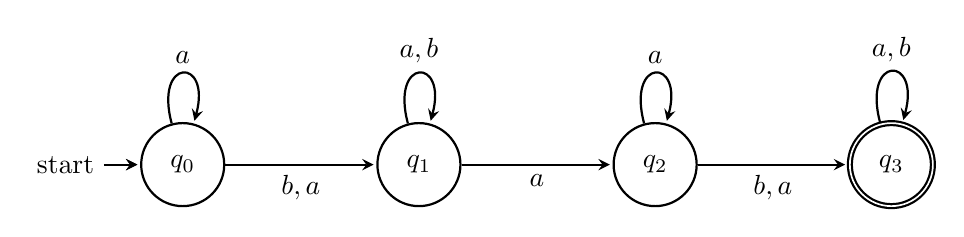
\begin{tikzpicture}[>=stealth, shorten >=1pt, node distance=3.0cm, on grid, auto, state/.append style={minimum size=3em}, thick ]
			\node[state, initial]				(A)               	{$q_0$};
			\node[state]						(B) [right of=A] 	{$q_1$};
			\node[state]				        (C) [right of=B] 	{$q_2$};
			\node[state, accepting]		        (D) [right of=C] 	{$q_3$};
			
			\path[->] (A) +(-1,0) edge (A)
			
			%Transições:
			%(Partida) edge [tipo da seta] node {simbolo lido} (Destino)
			(A) edge 			  				node [below] {$b,a$}	 (B)
			(A) edge [loop above]  				node 		 {$a$}		 ( )
			(B) edge 			  				node [below] {$a$}		 (C)
			(B) edge [loop above]  				node 		 {$a,b$}	 ( )
			(C) edge 			  				node [below] {$b,a$}	 (D)
			(C) edge [loop above]  				node 		 {$a$}	 	 ( )
			(D) edge [loop above]  				node 		 {$a,b$} 	 ( );
		\end{tikzpicture}
		\caption{Autômato para o exercício 12.}
		\label{fig:AutomaExercicioLR20}
	\end{figure}
	\begin{enumerate}
		\item Realize a computação para as palavras $aaba$ e $baba$.
		\item Esboce a árvore de computação para a palavra $abbaabaab$.
		\item Converta o AFN da Figura \ref{fig:AutomaExercicioLR20} para a notação algébrica.
		\item Encontre um AFD equivalente ao AFN da Figura \ref{fig:AutomaExercicioLR20}.
	\end{enumerate}
	
	\item Considerando o AFN representado pelo grafo de transição na Figura \ref{fig:AutomaExercicioLR21} responda o que é solicitado.
	
	\begin{figure}[h]
		\centering
		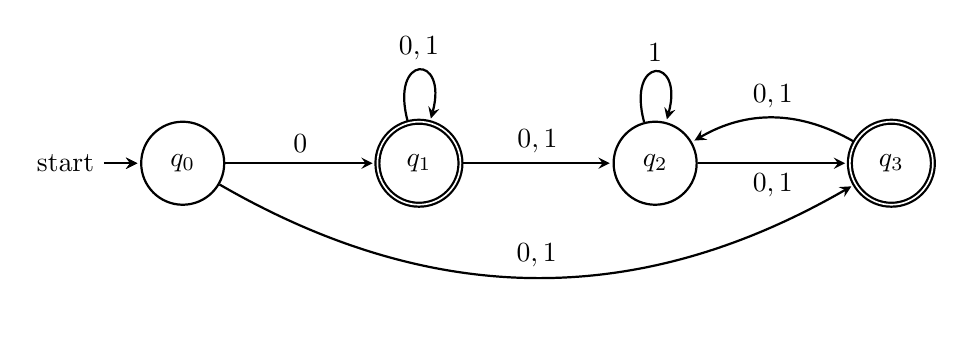
\begin{tikzpicture}[>=stealth, shorten >=1pt, node distance=3.0cm, on grid, auto, state/.append style={minimum size=3em}, thick ]
			\node[state, initial]				(A)               	{$q_0$};
			\node[state, accepting]				(B) [right of=A] 	{$q_1$};
			\node[state]				        (C) [right of=B] 	{$q_2$};
			\node[state, accepting]		        (D) [right of=C] 	{$q_3$};
			
			\path[->] (A) +(-1,0) edge (A)
			
			%Transições:
			%(Partida) edge [tipo da seta] node {simbolo lido} (Destino)
			(A) edge 			  				node {$0$}	 	 (B)
			(A) edge [bend right]  				node {$0,1$}	 (D)
			(B) edge [loop above]  				node {$0,1$}	 ( )
			(B) edge 			  				node {$0,1$} 	 (C)
			(C) edge [loop above]  				node {$1$}		 ( )
			(C) edge 							node [below] {$0,1$}	 (D)
			(D) edge [bend right]				node [above] {$0,1$}	 (C);
			
		\end{tikzpicture}
		\caption{Autômato para o exercício 14.}
		\label{fig:AutomaExercicioLR21}
	\end{figure}
	\begin{enumerate}
		\item Realize a computação para as palavras $01110$ e $1001011$.
		\item Esboce a árvore de computação para a palavra $110110101$.
		\item Converta o AFN da Figura \ref{fig:AutomaExercicioLR21} para a notação algébrica.
		\item Encontre um AFD equivalente ao AFN da Figura \ref{fig:AutomaExercicioLR21}.
	\end{enumerate}

	\item Considerando o $\lambda$-AFN do Exemplo \ref{exe:LinguagemLAFN1} responda o que é solicitado. 
	\begin{enumerate}
		\item Calcule $\delta_\lambda(q_0), \delta_\lambda(q_1)$ e $\delta_\lambda(q_2)$.
		\item Compute $\widehat{\underline{\delta_N}}(q_0, 11233)$.
		\item Apresente um AFD equivalente ao $\lambda$-AFN.
	\end{enumerate}

	\item Considerando $\Sigma_1 = \{0, 1\}$  e $\Sigma_2 = \{2, 3\}$ construa um $\lambda$-AFN com um único estado final que aceita a linguagem $\{w \in \Sigma_1^* \mid |w|_1 = 2i, i \in \mathbb{N}\} \cup \{w \in \Sigma_2^* \mid |w|_3 = 2j + 1, j\in \mathbb{N}\}$.
	
	\item Considere o alfabeto $\Sigma = \{a, b, c\}$ e as linguagens  $L_1 = \{w \in \Sigma^* \mid |w|_a \geq 0, |w|_b > 0, |w|_c = 2k, k \in \mathbb{N}\}$ e $L_2 = \{abaccc, ababc, abacab, acbcc, bacbaaa,$ $abb, bba, aaaabbbb, cac, ccba, caccabcac\}$. Para cada uma das linguagens $L_1 \cup L_2$, $L_1L_2$ e $L_2L_1$ construa um $\lambda$-AFN $A$ que as aceite.
	
	\item Considerando o $\lambda$-AFN $A = \langle Q, \Sigma, \underline{\delta_N}, q_0, \{q_2\} \rangle$ onde $\underline{\delta_N}$ é especificada pela Tabela \ref{tab:DeltaLAFN-Exe25}, responda o que é solicitado.
	
	\begin{table}[h]
		\centering
		\begin{tabular}{c|cccc}
			\backslashbox{$Q'$}{$\Sigma$}	& $\lambda$ & $a$ & $b$ & $c$\\\hline
			$q_0$ & $\emptyset$ & $\{q_0\}$ & $\{q_1\}$ & $\{q_2\}$\\
			$q_1$ & $\{q_0\}$ & $\{q_1\}$ & $\{q_2\}$ & $\emptyset$\\
			$q_2$ & $\{q_1\}$ & $\{q_2\}$ & $\emptyset$ & $\{q_0\}$ 		
		\end{tabular}
		\caption{Tabela da função de transição do $\lambda$-AFN do Exercício 18.}
		\label{tab:DeltaLAFN-Exe25}
	\end{table}

	\begin{enumerate}
		\item Para cada estado do autômato calcule $\delta_\lambda$.
		\item Esboce todos os $w$ pertencentes a linguagem do autômato tal que $|w| \leq 4$.
		\item Encontre um AFD equivalente $A$. 
	\end{enumerate}

	\item Considerando o $\lambda$-AFN $S = \langle Q, \Sigma, \underline{\delta_N}, s_0, \{s_2\} \rangle$ onde $\underline{\delta_N}$ é especificada pela Tabela \ref{tab:DeltaLAFN-Exe26}, responda o que é solicitado.
	
	\begin{table}[h]
		\centering
		\begin{tabular}{c|cccc}
			\backslashbox{$Q'$}{$\Sigma$}	& $\lambda$ & $0$ & $1$ & $2$\\\hline
			$s_0$ & $\{s_1, s_2\}$ & $\emptyset$  & $\{s_1\}$ & $\{s_2\}$\\
			$s_1$ & $\emptyset$ & $\{s_0\}$ & $\{s_2\}$ & $\{s_0, s_2\}$ \\
			$s_2$ & $\emptyset$ & $\emptyset$ & $\emptyset$ & $\emptyset$ 		
		\end{tabular}
		\caption{Tabela da função de transição do $\lambda$-AFN do exercício 19.}
		\label{tab:DeltaLAFN-Exe26}
	\end{table}

	\begin{enumerate}
		\item Para cada estado do autômato calcule $\delta_\lambda$.
		\item Esboce todos os $w$ pertencentes a linguagem do autômato tal que $|w| \leq 3$.
		\item Encontre um AFD equivalente $S$. 
	\end{enumerate}

	\item Para as linguagens especificadas pelos enunciados a seguir construa $\lambda$-AFN que as aceite.
	
	\begin{enumerate}
		\item A linguagem de todas as palavras que começam e terminam com qualquer letra do alfabeto $\{a,b,c\}$, porém não existe nas palavras dois $a$'s e dois $c$'s seguidos.
		\item A linguagem de todas as palavras sobre o alfabeto $\{0,1\}$ que iniciam com o prefixo $(01)^n$ e termina com o sufixo $10$ ou começam com o prefixo $(101)^n$ e terminam com o sufixo $00$, sendo $n \in \mathbb{N}$ tal que $n \geq 1$.
		\item A linguagem de todas as palavras sobre o alfabeto $\{x, y\}$ tal que no mínimo uma das quatro últimas letras da palavra é um $x$.
		\item A linguagem de todas as palavras sobre o alfabeto $\{x, y, z\}$ tal que no máximo uma das três primeiras letras da palavra é um $y$ ou as duas primeiras são $z$.
	\end{enumerate}

	\item Encontre o AFD quociente do AFD apresentado no Exercício 1.
	
	\item Encontre o AFD quociente equivalente ao AFN apresentado no Exercício 13.
	
	\item Encontre o AFD quociente equivalente ao AFN apresentado no Exercício 14.
	
	\item Encontre o AFD quociente equivalente ao $\lambda$-AFN apresentado no Exercício 18.
	
	\item Encontre o AFD quociente equivalente ao $\lambda$-AFN apresentado no Exercício 19.
	
	\item Encontre o AFD quociente equivalente ao $\lambda$-AFN da Figura \ref{fig:AutomaExercicioLR33} a seguir.
	
	\begin{figure}[h]
		\centering
		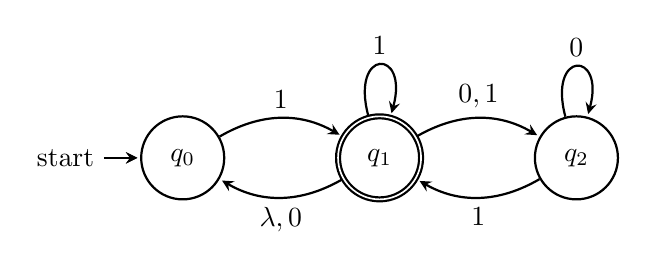
\begin{tikzpicture}[>=stealth, shorten >=1pt, node distance=2.5cm, on grid, auto, state/.append style={minimum size=3em}, thick ]
			\node[state, initial]				(A)               	{$q_0$};
			\node[state, accepting]				(B) [right of=A] 	{$q_1$};
			\node[state]				        (C) [right of=B] 	{$q_2$};
			
			\path[->] (A) +(-1,0) edge (A)
			
			%Transições:
			%(Partida) edge [tipo da seta] node {simbolo lido} (Destino)
			(A) edge [bend left]  				node {$1$}	 			 (B)
			(B) edge [bend left]  				node {$\lambda, 0$}		 (A)
			(B) edge [loop above]				node {$1$}				 ( )
			(B) edge [bend left]				node {$0,1$}			 (C)
			(C) edge [bend left]				node {$1$}				 (B)
			(C) edge [loop above]				node {$0$}				 ( );
		\end{tikzpicture}
		\caption{Autômato para o Exercício 26.}
		\label{fig:AutomaExercicioLR33}
	\end{figure}
	\newpage
	\item Encontre o AFD quociente equivalente ao $\lambda$-AFN da Figura \ref{fig:AutomaExercicioLR34} a seguir.
	
	\begin{figure}[h]
		\centering
		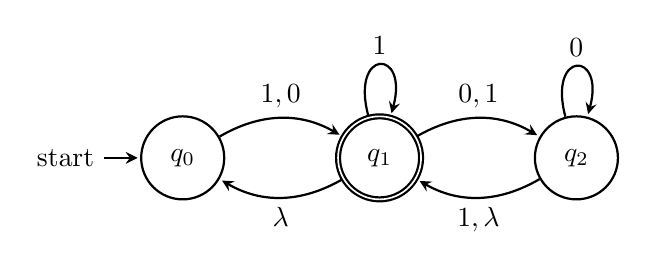
\begin{tikzpicture}[>=stealth, shorten >=1pt, node distance=2.5cm, on grid, auto, state/.append style={minimum size=3em}, thick ]
			\node[state, initial]				(A)               	{$q_0$};
			\node[state, accepting]				(B) [right of=A] 	{$q_1$};
			\node[state]				        (C) [right of=B] 	{$q_2$};
			
			\path[->] (A) +(-1,0) edge (A)
			
			%Transições:
			%(Partida) edge [tipo da seta] node {simbolo lido} (Destino)
			(A) edge [bend left]  				node {$1,0$} 			 (B)
			(B) edge [bend left]  				node {$\lambda$}		 (A)
			(B) edge [loop above]				node {$1$}				 ( )
			(B) edge [bend left]				node {$0,1$}			 (C)
			(C) edge [bend left]				node {$1, \lambda$}		 (B)
			(C) edge [loop above]				node {$0$}				 ( );
		\end{tikzpicture}
		\caption{Autômato para o Exercício 27.}
		\label{fig:AutomaExercicioLR34}
	\end{figure}

	\item Mostre uma expressão regular cuja valoração é exatamente a linguagem $\{aabb, aaabbb, aaba, \lambda\}$. 
	
	\item Construa uma expressão regular para cada uma das linguagens descrita no Exercício 3.
	
	\item Construa uma expressão regular para cada uma das linguagens descrita no Exercício 20.
	
	\item Para cada um dos AFD $A$, que foram criados por você para responder o Exercício 2, determine uma expressão regular $r$ tal que $\mathcal{L}(r) = \mathcal{L}(A)$.
	
	\item Para cada expressão regular a seguir construa um autômato que aceita a linguagem da expressão regular.
	\begin{enumerate}
		\item $a^*b + a$.
		\item $(ab + cd)^*$.
		\item $(a^*ab)^* + bc$.
		\item $(aa)^* (b + \lambda) + \emptyset$.
		\item $(a^*) + b(aa)^*$.
	\end{enumerate}
	
	\item Dado o alfabeto $\{a, b\}$ demonstre as asserções a seguir.
	\begin{enumerate}
		\item $(a + b)^* \equiv (a^*b^*)^*$.
		\item $a^* + b^* \not\equiv (a + b)^*$.
		\item $a^*b^* \not\equiv (ab)^*$.
		\item $(b + ab)^* (a + \lambda) \equiv (a + \lambda)(ba + b)^*$.
		\item $a^*a \equiv aa^*$.
		\item $\emptyset + (a + b)^* \equiv (a + b)^* + \emptyset$.
	\end{enumerate}

	\item Para quais quer $r_1, r_2, r_3 \in Exp_\Sigma$ demonstre as asserções a seguir.
	\begin{enumerate}
		\item $(r_1^*)^* \equiv r_1^*$.
		\item $(r_1 + r_2) \equiv r_2 + r_1$.
		\item $r_1 + (r_2 + r_3) \equiv (r_1 + r_2) + r_3$.
		\item $r_1 + r_1 \equiv r_1$.
		\item $(r_1 + r_2)^* \equiv (r_1^* r_2^*)^*$.
		\item $r_1r_1 \equiv r_1$.
		\item $(r_1r_2)^*r_1 \equiv r_1(r_2r_1)^*$.
		\item $r_1 + \emptyset \equiv r_1$.
	\end{enumerate}

	\item Construa um autômato que aceite cada valoração a seguir.
	\begin{enumerate}
		\item $\mathcal{L}(aa^*(b + a))$.
		\item $\mathcal{L}((aa + abb)^*(aa + \lambda + ba))$.
		\item $\mathcal{L}((ab + b)^*(a + \lambda))$.
		\item $\mathcal{L}(aa^* + aba^*b^*)$.
		\item $\mathcal{L}((\lambda + \emptyset)^*)$.
		\item $\mathcal{L}(aa^*bb^*aa^*)$.
		\item $\mathcal{L}(ab + (\emptyset + a)^*b)$.
		\item $\mathcal{L}((a^*(b(bb)^*aa)^*)a)$.
		\item $\mathcal{L}(((aa)^*)^*)$.
		\item $\mathcal{L}((b + a)(\lambda^*)^*)$.
		\item $\mathcal{L}(a^*(ba + ab))$.
		\item $\mathcal{L}((bb + bab)^*(a + \lambda aa^* + ba))$.
		\item $\mathcal{L}((b^* + b)^*(a^* + \lambda))$.
		\item $\mathcal{L}(a^* + ba)$.
		\item $\mathcal{L}(((\lambda)^* + \emptyset)^*)$.
		\item $\mathcal{L}(a^*ba^*ba^*)$.
		\item $\mathcal{L}(bab + (ab + a)b)$.
		\item $\mathcal{L}(a(b)^*b^*)$.
		\item $\mathcal{L}((b + a)(b + a)$.
	\end{enumerate}

	\item Construa uma expressão regular cuja valoração seja exatamente a linguagem aceita pelo AFD da Figura \ref{fig:AutomaExercicioLR8}.
	
	\item Construa uma gramática regular à esquerda para cada uma das linguagens descrita no Exercício 3.
	
	\item Construa uma gramática regular à direita para cada uma das linguagens descrita no Exercício 3.
	
	\item Construa uma gramática regular à esquerda para cada uma das linguagens descrita no Exercício 20.
	
	\item Construa uma gramática regular à direita para cada uma das linguagens descrita no Exercício 20.
	
	\item Construa uma gramática regular que gera exatamente cada valoração a seguir.
	\begin{enumerate}
		\item $\mathcal{L}(a^*b + a)$.
		\item $\mathcal{L}((ab + cd)^*)$.
		\item $\mathcal{L}((a^*ab)^* + bc)$.
		\item $\mathcal{L}((aa)^* (b + \lambda))$.
		\item $\mathcal{L}((a^*) + b(aa)^*)$.
	\end{enumerate}

	\item Construa uma gramática regular que gera exatamente a linguagem aceita pelo AFD da Figura \ref{fig:AutomaExercicioLR8}.
	
	\item Para as gramáticas descrita a seguir construa um AFN que aceita as linguagens geradas por tais gramáticas. 
	\begin{enumerate}
		\item $G_1 = \langle \{S, A, B\},\{a, b\}, S, P \rangle$ onde $P$ é definido por, 
		\begin{eqnarray*}
			S & \rhd & aA \mid bB \mid aaS \mid bbS\\
			A & \rhd & aA \mid \lambda \\
			B & \rhd & bB \mid b
		\end{eqnarray*}
		
		\item $G_2 = \langle \{S, A, B\},\{a, b\}, S, P \rangle$ onde $P$ é definido por, 
		\begin{eqnarray*}
			S & \rhd & abA\\
			A & \rhd & bab\\
			B & \rhd & aA \mid bb
		\end{eqnarray*}
		
		\item $G_3 = \langle \{S, A, B\},\{a, b\}, S, P \rangle$ onde $P$ é definido por, 
		\begin{eqnarray*}
			S & \rhd & aA \mid bS \mid \lambda\\
			A & \rhd & aB \mid bS \mid \lambda \\
			B & \rhd & aaS \mid bS \mid \lambda 
		\end{eqnarray*}
		
		\item $G_4 = \langle \{S, A\},\{a, b\}, S, P \rangle$ onde $P$ é definido por,
		\begin{eqnarray*}
			S & \rhd & aaB \mid b\\
			A & \rhd & bbS 
		\end{eqnarray*}
		
		\item $G_5 = \langle \{S, A, B\},\{a, b\}, S, P \rangle$ onde $P$ é definido por, 
		\begin{eqnarray*}
			S & \rhd & aaaA \mid bbB\\
			A & \rhd & abaA \mid S\\
			B & \rhd & bbS \mid aA \mid bb\\ 
		\end{eqnarray*}
	\end{enumerate}

	\item Para cada gramática do Exercício 43 esboce uma gramática regular unitária à esquerda equivalente.
	
	\item Esboce uma gramática regular que gere a linguagem aceita pelo AFD da Figura \ref{fig:AFD-Expressao}. 
	
\end{problemset}
	
\chapter{Linguagens Livres do Contexto}\label{cap:LinguagemLLC}

\begin{introduction}[Tópicos]
	\item Gramática Livres do Contexto
	\item Simplificação e Formas Normais de GLC
	\item Sobre Algoritmos de Pertinência em GLC
	\item GLC e Linguagens de Programação
	\item Autômato de Pilha Determinístico
	\item Autômato de Pilha Não-determinístico
	\item Álgebra das Linguagens Livres de Contexto
	\item Questionário
\end{introduction}

No capítulo passado foram apresentadas três diferentes formalismos para a classe das linguagens regulares, a saber, o formalismo operacional (os autômatos), o formalismo denotacional (as expressões regulares) e por fim o formalismo gerador ou axiomático (as gramáticas regulares). Agora este manuscrito irá continuar o estudo das linguagens formais apresentando a classe das linguagens livres do contexto, como antes serão apresentados diferentes formalismo para tal classe de linguagens.

\section{Gramática Livres do Contexto}\label{sec:GLC}

O estudo das Linguagens Livres do Contexto será iniciado aqui pela apresentação de seu formalismo gerador, ou seja, será primeiro apresentado a noção de Gramática Livre do Contexto.

\begin{definition}[Gramática Livre do Contexto]\label{def:GLC}
	\cite{benjaLivro2010} Uma Gramática Livre do Contexto, ou simplesmente GLC, é uma gramática formal $G = \langle V, \Sigma, S, P\rangle$ onde todo $\alpha \rhd \beta \in P$ é tal que $\alpha \in V$ e $\beta \in (V \cup \Sigma)^*$.
\end{definition}

\begin{example}\label{exe:GLC-1}
	A estrutura $G = \langle \{A, B, C\}, \{0,1\}, A, P\rangle$ onde $P$ é definido pela regras:
	\begin{eqnarray*}
		A & \rhd & A0110BC \mid 0110C \mid AAB0110CC \mid \lambda\\
		B & \rhd & 01B10 \mid 0110\\
		C & \rhd & 01C \mid \lambda
	\end{eqnarray*}
	é uma GLC.
\end{example}

Obviamente o leitor atento pode notar que a Definição \ref{def:GLC} garante que toda Gramática Regular é um caso particular de GLC, porém o inverso não é verdadeiro, basta notar que a gramática apresentada no Exemplo \ref{exe:GLC-1}, fere a definição de gramática regular apresentada na Seção \ref{sec:GramaticaRegular} do capítulo passado. Agora utilizando a Definição \ref{def:LinaugemGramatica} pode-se formalizar o conceito de Linguagem Livre do Contexto.

\begin{definition}[Linguagem Livre do Contexto]\label{def:LLC}
	A linguagem $L$ gerada por uma GLC $G$, ou seja, $L = \mathcal{L}(G)$, será chamada de Linguagem Livre do Contexto, ou simplesmente LLC.
\end{definition}

Como para os casos das linguagens reconhecidas por AFD, para provar que uma determinada GLC $G$ gera uma linguagem $L$ é necessário demonstrar o seguinte resultado $w \in L \Longleftrightarrow w \in \mathcal{L}(G)$.

\begin{example}\label{exe:LinguagemGLC}
	A linguagem $L = \{a^ib^i \mid i  > 0\}$ é gerado pela GLC $G = \langle \{S\}, \{a,b,c\}, S, P\rangle$ onde $P$ é formado pelas regras,
	\begin{eqnarray*}
		S & \rhd & aSb \mid ab
	\end{eqnarray*}
	\begin{proof}
		$(\Rightarrow)$ Suponha que $w \in L$ assim $w = a^ib^i$ para $i  > 0$, agora por indução sobre a quantidade $n$ de derivações em $G$ será mostrado que toda forma sentencial gerada por $G$ é da forma $a^nS^jb^n$ com $j \in \{0, 1\}$. 
		\begin{itemize}
			\item[ ] \textbf{Base da indução}: Com $n = 1$, é trivial pelas regras em $P$. 
			\item[ ] \textbf{Hipótese indutiva (HI)}: Assuma que com $n$ derivações tal que $n \geq 0$ a forma sentencial $a^nS^jb^n$ é gerada pela GLC $G$, ou seja, $S \gg^n a^nS^jb^n$ com $j \in \{0, 1\}$. 
			\item[ ] \textbf{Passo indutivo}: Agora dado $S \gg^{n+1} w'$, ou seja, $w'$ é derivada de $S$ com $n+1$ derivações, assim por definição tem-se que existe $w''$ tal que $S \gg^n w'' \gg w'$, mas por \textbf{(HI)} tem-se que $w'' =  a^nS^jb^n$ com $n \geq 0$ e $j \in \{0, 1\}$,  desde que, $w'$ é gerada de $w''$ é claro que $j = 1$, ou seja, $w'' = a^nSb^n$, consequentemente, $w' = a^{n+1}Sb^{n+1}$ ou $w' = a^{n+1}b^{n+1}$ e, portanto, $w'$ é da forma $a^{n+1}S^jb^{n+1}$ com $j \in \{0, 1\}$. 
		\end{itemize}
		Agora por hipótese tinha-se que $w = a^ib^i$ para $i  > 0$, ou seja, $w = a^iS^0b^i$, dessa forma pela indução acima $w$ é uma forma sentencial gerada por $G$, e como $w \in \Sigma^*$ tem-se por definição que $w \in \mathcal{L}(G)$. $(\Rightarrow)$ Suponha que $w \in \mathcal{L}(G)$, agora será mostrado por indução sobre a quantidade $n$ de derivações que todo $w$ gerado por $G$ estará em $L$.
		\begin{itemize}
			\item[ ] \textbf{Base da indução:} Com $n=1$, ou seja, como uma única derivação, pelo fato de que $w \in \Sigma^*$ e pelas regras em $P$ tem-se obrigatoriamente que $w = ab$ e, portanto, $w = a^1b^1$ , consequentemente, $w \in L$.
			\item[ ] \textbf{Hipótese indutiva (HI)}: Assuma que para todo $S \gg^n w$ tal que $n \geq 1$, tem-se que $w \in L$.
			\item[ ] \textbf{Passo indutivo}: Agora dado $S \gg^{n+1} w$, ou seja, $w$ é derivado em $G$ com $n + 1$ derivações de forma que $n \geq 1$. Desde que $n  \geq 1$ tem-se que $n + 1  > 1$, assim a palavra $ab$ não pode ser $w$ uma vez que são usadas pelo menos duas derivações para gerar $w$. Assim a derivação de $w$ deverá ter sido iniciado usando a regra $S \rhd aSb$ e, portanto, $w = aw'b$ em que $S \gg^n w'$, mas pela hipótese indutiva $w' \in L$, logo $w' = a^ib^i$ com $i > 0$, consequentemente $w = aa^ib^ib = a^{i+1}b^{i+1}$, logo $w \in L$.
		\end{itemize}
	\end{proof}
\end{example}

Note que para a prova mostrada no Exemplo \ref{exe:LinguagemGLC} foi-se usada indução sobre o tamanho das derivações, isto não é a única forma de se proceder para provar que uma gramática gera uma determinada linguagem, de  fato como apresentado em \cite{hopcroft2008} pode-se usar a ideia de indução sobre as árvores de derivações (apresentadas mais a frente), neste manuscrito não será apresentado tal estratégia, porém fica a referência para interessados no tema. 

Nas GLC que não são lineares, ou seja, as gramática em que as regras em $P$ podem conter duas ou mais variáveis do lado direto do símbolo $\rhd$, é permitido a escolha sobre qual variável ser derivada primeiramente, para ilustrar isso considere uma forma sentencial $0A10BC$ e as regras $A \rhd 00, B \rhd \lambda$ e $C \rhd 1$, note que dependendo de qual variável é escolhida para ser reescrita a próxima forma sentencial pode assumir três formas diferentes. Apresentado esta ideia pode-se agora formalizar o conceito de reescrita \textbf{mais à esquerda} e \textbf{mais à direita}.

\begin{definition}[Tipos de Derivação]\label{def:TiposLateraisReescrita}
	Dado uma GLC $G = \langle V, \Sigma, S, P\rangle$ e seja $w_1A_1w_2\cdots w_nA_nw_{n+1}$ uma forma sentencial derivável em $G$ tal que $w_i \in \Sigma^*$ e $A_j \in V$ para todo $1 \leq i \leq n+1$ e $1 \leq j \leq n$. Uma derivação é dita mais à esquerda (à direita) se ela é da forma $w_1A_1w_2\cdots w_nA_nw_{n+1} \gg w_1w'w_2\cdots w_nA_nw_{n+1}$ ($w_1A_1w_2\cdots w_nA_nw_{n+1} \gg w_1A_1w_2\cdots w_nw'w_{n+1}$)  com  $w' \in (V \cup \Sigma)^*$.
\end{definition}

\begin{example}\label{exe:ReescritasLaterais}
	Considere a GLC $G = \langle \{S, A, B\}, \{0, 1\}, S, P\rangle$ em que $P$ é formado pelas regras,
	\begin{eqnarray*}
		S & \rhd & 0AB\\
		A & \rhd & 11B1 \\
		B & \rhd & A \mid \lambda 
	\end{eqnarray*}
	claramente a palavra $011B1A$ é um forma sentencial derivável em $G$, agora note que:
	\begin{eqnarray*}
		011B1A & \gg & 011A1A\\
		011B1A & \gg & 0111A
	\end{eqnarray*}
	são ambas derivações mais à esquerda, e 
	\begin{eqnarray*}
		011B1A & \gg & 011B111B1
	\end{eqnarray*}
	é uma derivação mais à direita.
\end{example}

\begin{definition}[Tipo de Geração]\label{def:TipoGeracao}
	Dado uma GLC $G = \langle V, \Sigma, S, P\rangle$,  uma derivação $S \gg^* w$ é dita ser uma geração mais à esquerda (à direita) sempre que $w \in \Sigma^*$ e toda derivação realizada for mais à esquerda (à direita).
\end{definition}

\begin{example}\label{exe:TipoGeracao}
	Considere a gramática do Exemplo \ref{exe:ReescritasLaterais} a derivação, 
	$$S \gg 0AB \gg 011B1B \gg 0111B \gg 0111$$
	é claramente uma geração mais à esquerda, já a derivação
	$$S \gg 0AB \gg 0A \gg 011B1 \gg 0111$$
	é notavelmente uma geração mais à direita.
\end{example}

\begin{remark}
  Resumindo dado uma GLC $G = \langle V, \Sigma, S, P\rangle$ uma geração é obrigatoriamente uma derivação $S \gg w$ em que $w \in \Sigma^*$, ou seja, uma derivação que gera (ou produz) uma palavra sobre o alfabeto $\Sigma$.
\end{remark}

Além da noção de geração, para visualizar o passo a passo da ``construção'' de uma palavra $w \in \Sigma^*$ em uma GLC $G$ é comum usar a ideia de árvore de derivação\footnote{Na literatura como no livro \cite{benjaLivro2010} também é comum encontrar a nomenclatura árvore ordenada.}. 

Uma árvore de derivação nada mais é do que uma forma visual estruturada em uma árvore\footnote{As árvores de derivação são representações cuja a forma similar a construção das árvores $n$-árias da área de estrutura de dados \cite{jaime1994}.} que representar a construção de uma palavra, em que cada nível da árvore representa é gerada pela aplicação de uma ou mais regras de reescrita, neste sentido as folhos da árvore contém os símbolos da palavra $w$.

\begin{definition}[Árvore de Derivação]\label{def:ArvoreGLC}
	Seja $G = \langle V, \Sigma, S, P\rangle$ uma GLC e dado $w \in \mathcal{L}(G)$, uma árvore de derivação para $w$ é construída seguindo as seguintes regras:
	\begin{enumerate}
		\item O símbolo $S$ é a raiz da árvore.
		\item Todo símbolo $a \in \Sigma \cup \{\lambda\}$ é o rótulo de uma folha.
		\item Todo símbolo $A \in V$ é o rótulo de uma raiz de uma sub-árvore\footnote{Aqui sub-árvore e no mesmo sentido que o leitor já deve ter visto em estrutura de dados.}.
		\item Se $A$ é uma raiz e seus ``filhos'' são  $x_1, \cdots, x_n$ com $x_i \in V \cup \Sigma \cup \{\lambda\}$ para $1 \leq i \leq n$, então existe em $P$ uma regra da forma $A \rhd x_1\cdots x_n$.
		\item Todo folha rotulada por $\lambda$ de uma raiz $A$ será filho único, ou seja, em $P$ existe uma regra da forma $A \rhd \lambda$.
	\end{enumerate}
\end{definition}

\newpage
\begin{example}\label{exe:ArvoreGLC1}
	Tem-se que a derivação $S \gg 0AB \gg 011B1B \gg 0111B \gg 0111$ apresentada no Exemplo \ref{exe:TipoGeracao} é representada pela árvore esboçada na Figura \ref{fig:ArvoreGLC1} a seguir.
	
	\begin{figure}[h]
		\centering
		\begin{tikzpicture}[sibling distance=.6cm, empty/.style={draw=none}, tlabel/.style={font=\footnotesize\color{red!70!black}}]
			\Tree   [.$S$  
					[.$0$ ]
						%\edge node[tlabel,auto=left] {1}; 
					[.$A$  
							[.$1$ ]
							[.$1$ ]
							[.$B$ 
								{$\lambda$}
							] 
							[.$1$ ]
					] 
					[.B   
						%\edge[empty]; {} \edge node[tlabel,auto=left] {5}; {b}   
						{$\lambda$}
					]
			]
		\end{tikzpicture}
		\caption{Árvore para a derivação $S \gg 0AB \gg 011B1B \gg 0111B \gg 0111$.}
		\label{fig:ArvoreGLC1}
	\end{figure}
\end{example}

\begin{example}\label{exe:ArvoreGLC2}
	Tem-se que a derivação $S \gg 0AB \gg 0A \gg 011B1 \gg 0111$ apresentada no Exemplo \ref{exe:TipoGeracao} é representada pela árvore esboçada na Figura \ref{fig:ArvoreGLC2} a seguir.
	
	\begin{figure}[h]
		\centering
		\begin{tikzpicture}[sibling distance=.6cm, empty/.style={draw=none}, tlabel/.style={font=\footnotesize\color{red!70!black}}]
			\Tree [.$S$  
					[.$0$ ]
					[.$A$
						[.$1$ ] 
						[.$1$ ] 
						[.$B$ 
							{$\lambda$}
						] 
						[.$1$ ] 
					]
					[.$B$
						{$\lambda$} 
					]
			]
		\end{tikzpicture}
		\caption{Árvore para a derivação $S \gg 0AB \gg 0A \gg 011B1 \gg 0111$.}
		\label{fig:ArvoreGLC2}
	\end{figure}
\end{example}

\begin{remark}
	Os Exemplos \ref{exe:ArvoreGLC1} e \ref{exe:ArvoreGLC2} mostram que que diferentes derivações podem ser representadas pela mesma árvore, isso acontece devido ao fato de que a árvore de derivação apenas esboça o processo de formação total (ou final), e não o comportamento (ou momento) parcial das derivação.
\end{remark}

\begin{note}
	Em algumas obras tais como \cite{benjaLivro2010} as folhas e raízes nas árvores de derivação são gravados com círculos, neste manuscrito isso não será feito para não confundir o leitor iniciante com a representação visual dos autômatos finitos.
\end{note}

\begin{definition}[Ambiguidade]\label{def:AmbiguidadePalavra}
	Dado uma GLC $G = \langle V, \Sigma, S, P\rangle$ uma palavra $w \in \mathcal{L}(G)$ é dita ser ambígua sempre que existe duas gerações diferentes para $w$.
\end{definition}

A Definição \ref{def:AmbiguidadePalavra} pode ser reinterpretada da seguinte forma: uma palavra $w$ é ambígua com relação a uma GLC $G$ se existem duas gerações mais à esquerda (à direta) para tal palavra.

\begin{definition}[Linguagem Ambígua]\label{def:LinguagemAmbiguidade}
	Uma linguagem $L$ é dita ser ambígua se existe uma GLC $G$ e uma palavra $w$ tal que $L = \mathcal{L}(G)$ e $w$ seja uma palavra ambígua em $G$. L será dita inerentemente ambígua se existe $w$ para todo GLC $G$ tal que  $w$ seja uma palavra ambígua em $G$ e $L = \mathcal{L}(G)$.
\end{definition}

\begin{example}
	Considere a GLC $G = \langle \{S\}, \{a, b\}, S, P \rangle$ onde $P$ é o formado pelas seguintes regras:
	\begin{eqnarray*}
		S & \rhd & aSb \mid SS \mid \lambda
	\end{eqnarray*}
	a palavra $aabb$ é ambígua, pois existem as duas árvores de derivação apresentadas na Figura \ref{fig:ArvoresAmbuigas}, assim tem-se que $\mathcal{L}(G)$ é uma linguagem ambígua.
	
	\begin{figure}[h]
		\centering
		\subfloat[Primeira ávore.]{
			\begin{tikzpicture}[sibling distance=.8cm, empty/.style={draw=none}, tlabel/.style={font=\footnotesize\color{red!70!black}}]
				\Tree [.$S$  
						[.$a$ ]
						[.$S$
							[.$a$ ] 
							[.$S$
								{$\lambda$} 
							] 
							[.$b$ ] 
						]
						[.$b$ ]
				]
			\end{tikzpicture}
			\label{Ima:Arvore1}
		}\hfill
		\subfloat[Segunda ávore.]{
			\begin{tikzpicture}[sibling distance=.8cm, empty/.style={draw=none}, tlabel/.style={font=\footnotesize\color{red!70!black}}]
				\Tree [.$S$  
						[.$S$
							{$\lambda$} 
						]
						[.$S$
							[.$a$ ]
							[.$S$
								[.$a$ ] 
								[.$S$
									{$\lambda$} 
								] 
								[.$b$ ] 
							]
							[.$b$ ] 
						]
				]
			\end{tikzpicture}
			\label{Ima:Arvore2}
		}%
		\caption{As árvores de derivação para a palavra $aabb$}
		\label{fig:ArvoresAmbuigas}
	\end{figure}
\end{example}

Ambiguidade é uma característica comum encontrada nas linguagem naturais \cite{benjaLivro2010} e em tais linguagens essa característica é tolerada, em contrapartida, as linguagens de programação não toleram muito bem o aspecto da ambiguidade assim em geral a mesma deve ser sempre que possível evitada ou eliminada. Uma estratégia comum para a eliminação da ambiguidade em linguagens de programação é estabelecer prioridade na geração de certos símbolos da linguagens \cite{benjaLivro2010, aho2007}. 

\section{Simplificação de Gramática Livres do Contexto}\label{sec:SimplficacaoGLC}

Antes de apresentar as regras de simplificação e alguns resultados sobre as mesmas é conveniente discutir alguns aspectos sobre as GLC. Antes de tudo lembre que na definição de GLC (Definição \ref{def:GLC}) não existe qualquer restrição para a forma das palavras encontradas à direita das regras de reescrita. Assim podem haver $n$ variáveis, recursão, geração de $\lambda$ e etc. Algumas desta, entretanto, podem ser removidas ou alteradas de forma que a gramática possa ser mais simples de ser utilizada, e será isto que será estudado nesta seção, ou seja, aqui será estudado diversas estratégias para transformar uma gramática qualquer $G$ em uma gramática $G'$ com alguns restrições, mas que preserva a linguagem gerada, isto é, $\mathcal{L}(G) = \mathcal{L}(G')$. 

\begin{remark}
    Assim como em \cite{benjaLivro2010} as gramáticas que serão consideradas nesta seção não são capazes de gerar a palavra vazia, ou seja, $S \not\gg \lambda$ ou ainda $\lambda \notin \mathcal{L}(G)$. Entretanto isso não irá diminuir em nada a força dos resultados que serão obtidos aqui.
\end{remark}

\begin{definition}[Regra da substituição]\label{def:RegraSubstituicao}
    Seja $G = \langle V, \Sigma, S, P\rangle$ uma GLC e seja $A, B \in V$ tal que $A \neq B$ de forma que em $P$ existem as produções:
    $$A \rhd x_1Bx_2$$
    e
    $$B \rhd y_1 \mid y_2 \mid \cdots \mid y_n$$
    a regra de substituição consiste em para cada a regra $A \rhd x_1A x_2$ em $P$ adicionar as regras:
    $$A \rhd x_1y_1x_2 \mid x_1y_2x_2 \mid \cdots \mid x_1y_nx_2 \mid$$.
\end{definition}

Note que a regra de substituição de fato só altera a forma do conjunto $P$ gerando um novo conjunto $P'$, e pela própria regra é fácil notar que vale a seguinte desigualdade $\# P \leq \# P'$. 

\begin{theorem}\label{teo:SuplificacaoGLC-Sub}
    Se $G = \langle V, \Sigma, S, P\rangle$ é uma GLC, então a gramática $G'$ gerada a partir da regra de substituição é tal que $\mathcal{L}(G) = \mathcal{L}(G')$.
\end{theorem}

\begin{proof}
    Suponha $G = \langle V, \Sigma, S, P\rangle$ é uma GLC, agora seja $G' = \langle V, \Sigma, S, P'\rangle$ a GLC gerada a partir da regra de substituição aplicada a $G$. Agora assuma que $w \in \mathcal{L}(G)$, ou seja, $S \gg_G^* w$, dessa forma há dois casos para serem considerados:
    \begin{itemize}
        \item[(1)] Se durante a derivação $S \gg_G^* w$ não forem usadas regras da forma $A \rhd x_1Bx_2$, então obviamente essa mesma derivação pode ser replicada em todos os seu detalhes na gramática $G'$, uma vez que, todas as regras que não são da forma $A \rhd x_1Bx_2$ estão também em $P'$, assim $S \gg_{G'}^* w$, consequentemente, $w \in \mathcal{L}(G')$.
        \item[(2)] Agora sem perda de generalidade assuma que pelo menos uma regra da forma  $A \rhd x_1Bx_2$ seguida da regra $B \rhd y_1$ aparecem na derivação $S \gg_G^* w$, portanto, tem-se que:
        $$S \gg_G^* k_1Ak_2 \gg_{G} k_1x_1Bx_2k_2 \gg_{G} k_1x_1y_1x_2k_2 \gg^*_G w $$
        com $k_1, k_2, x_1, x_2, y_1 \in (V \cup \Sigma)^*$. Assim pela construção de $G'$ pode-se então realizar a seguinte derivação:
        $$S \gg^*_{G'} k_1Ak_2 \gg_{G'} k_1x_1y_1x_2k_2  \gg^*_{G'} w$$
        e assim tem-se que, $w \in \mathcal{L}(G')$.
    \end{itemize}
    Logo pelos casos $(1)$ e $(2)$ acima tem-se que $\mathcal{L}(G) \subseteq \mathcal{L}(G')$. Agora mostrar que $\mathcal{L}(G') \subseteq \mathcal{L}(G)$ é trivial e não será feito aqui, e desde que $\mathcal{L}(G) \subseteq \mathcal{L}(G')$ e $\mathcal{L}(G') \subseteq \mathcal{L}(G)$ por definição tem-se que $\mathcal{L}(G) = \mathcal{L}(G')$ o que completa a prova.
\end{proof}

Como pode ser visto no Teorema \ref{teo:SuplificacaoGLC-Sub} e como discutido em \cite{benjaLivro2010} a regra de substituição pode até aumentar o número de regras de reescrita, porém, a mesma também permite que seja realizadas geração mais rápidas, isto é, que aconteçam derivações de palavras $w \in \Sigma^*$ com menos passos.

\begin{example}
    Dado a GLC $G = \langle \{S, A, B, C\}, \{0,1\}, S, P \rangle$ com $P$ definido pelas regras:
    \begin{eqnarray*}
        S & \rhd & A001 \mid B100\\
        A & \rhd & 01 \mid 01B\\
        B & \rhd & 1 \mid 0 \mid \lambda
    \end{eqnarray*}
    aplicando a regra de substituição em tal gramática será gerada na gramática $G' = \langle \{S, A, B, C\}, \{0,1\}, S, P' \rangle$ em que $P'$ corresponde ao conjunto formado pela seguintes regras:
    \begin{eqnarray*}
        S & \rhd & A001 \mid B100 \mid  01001 \mid 01B001 \mid 1100 \mid 0100 \mid 100 011001 \mid 010001 \mid 01001\\
        A & \rhd & 01 \mid 01B \mid 011 \mid  010 \\
        B & \rhd & 1 \mid 0 \mid \lambda
    \end{eqnarray*}
\end{example}

Para prosseguir com o estudo das regras de simplificação antes é necessário formalizar o conceito de variável recursiva à esquerda nas GLC.

\begin{definition}[Regra Recursiva à Esquerda]\label{def:VariavelRecursiva}
    Seja $G = \langle V, \Sigma, S, P\rangle$ uma GLC, uma variável $A$ é dita recursiva à esquerda se existe pelo menos uma regra $A \rhd Ax \in P$ com  $A \in V$ e $x \in (V \cup \Sigma)^*$.
\end{definition}

Agora é possível formalizar então a próxima regra de simplificação de GLC, sendo esta próxima regra nomeada como \textbf{Regra de Remoção da Recursividade Esquerda}.

\begin{definition}[Regra de Remoção da Recursividade Esquerda]\label{def:RegraRecursiva}
    Seja $G = \langle V, \Sigma, S, P\rangle$ uma GLC com variáveis recursivas à esquerda. Então substitua para cada $A \in V$ as regras:
    $$A \rhd Ax_1 \mid \cdots \mid Ax_m \mid y_1 \mid \cdots \mid y_n$$
    pelas regras:
    \begin{eqnarray*}
        A & \rhd & y_1 \mid \cdots \mid y_n \mid y_1Z \mid \cdots \mid y_nZ\\
        Z & \rhd & x_1 \mid \cdots \mid x_m \mid x_1Z \mid \cdots \mid x_mZ
    \end{eqnarray*}
	onde $x_1, \cdots, x_m, y_1, \cdots, y_n \in (V \cup \Sigma)^*$ e $Z$ é uma variável nova que deve ser adicionada ao conjunto $V$.
\end{definition}

Fica claro pela definição da Regra de Remoção da Recursividade Esquerda que após usa aplicação será gerada uma nova gramática com mais varáveis que a gramática original terá uma quantidade igual ou superior de regras de reescritas.

\begin{theorem}\label{teo:SuplificacaoGLC-Rec}
    Se $G = \langle V, \Sigma, S, P\rangle$ é uma GLC, então a gramática $G'$ gerada a partir da regra de remoção da recursividade esquerda é tal que $\mathcal{L}(G) = \mathcal{L}(G')$.
\end{theorem}

\begin{proof}
    Ficará como exercício ao leitor.
\end{proof}

\begin{example}
    Dado a GLC $G = \langle \{S, A\}, \{a,b, c\}, S, P \rangle$ com $P$ definido pelas regras:
    \begin{eqnarray*}
        S & \rhd & aSc \mid aAc\\
        A & \rhd & Ab \mid b
    \end{eqnarray*}
    Usando a regra de remoção da recursividade esquerda é obtida a GLC $G = \langle \{S, A, B\}, \{a, b, c\}, S, P' \rangle$ onde $P'$ é definido por:
    \begin{eqnarray*}
        S & \rhd & aSc \mid aAc\\
        A & \rhd & b \mid bB\\
        B & \rhd & b \mid bB 
    \end{eqnarray*}
\end{example}

Agora para continuar com o estudo das regras de simplificação será necessário formalizar três conceitos chaves, o primeiro conceito é a noção de relação (ou grafo) de dependências, a saber tais relações (ou grafos) são ferramentas advindas da teoria dos grafos e frequentemente usada em muitos campos do conhecimento para modela sistemas complexos \cite{benjaLivro2010}, a seguir este conceito será apresentado de forma rigorosa com respeito as GLC.

\begin{definition}[Relação de dependência]\label{def:GrafoDependencia}
    Seja $G = \langle V, \Sigma, S, P\rangle$ é uma GLC, a relação de dependência $DEP$ é construída como: $(A, B) \in DEP$ se, e somente se, $A \rhd xBy \in P$ com $x, y \in (V \cup \Sigma)^*$ e $A \neq B$.
\end{definition}

O leitor pode considerar a relação $DEP$ como sendo uma relação de necessidade, em que $(A, B) \in DEP$ pode ser semanticamente interpretado como, para escrever $B$ é necessário que antes existem um $A$.

\begin{remark}
    Para fins de notação, será usado o rótulo $\widehat{DEP}$ para denotar o fecho transitivo da relação $DEP$.
\end{remark}

\begin{example}\label{exe:GLCDEP}
    Considere a GLC $G = \langle \{A, B, C, D, E\}, \{0, 1\}, A, P \rangle$ onde $P$ é o conjunto formado pelas regras:
    
    \begin{eqnarray*}
        A & \rhd & 00A \mid 0B1 \mid 10AB \mid AD\\ 
        B & \rhd & 1B01 \mid D01E\mid \lambda\\
        C & \rhd & C01 \mid 00101 \mid 1 \mid \lambda\\
        D & \rhd & 01E \mid 0E\\
        E & \rhd & 1E0 \mid EE \mid D
    \end{eqnarray*}
    Tem-se que $\widehat{DEP}$ é o conjunto formado pelo pares $(A, B), (A, D), (B, D), (B, E), (D, E),$ e $(E, D)$.
\end{example}

O próximo conceito necessário é a noção de variável inacessível formalizado a seguir.

\begin{definition}[Variável inacessível]\label{def:VariavelInacessível}
    Seja $G = \langle V, \Sigma, S, P\rangle$ é uma GLC, uma variável $A \neq S$ é dita ser inacessível sempre que $(S, A) \notin \widehat{DEP}$.
\end{definition}

\begin{example}
    Considere a GLC apresentada no Exemplo \ref{exe:GLCDEP}, em tal gramática é fácil notar que a variável $C$ é inacessível.
\end{example}

\begin{lemma}\label{lema:SemInacessivel}
    Se $G = \langle V, \Sigma, S, P\rangle$ é uma GLC, então existe uma GLC sem variáveis inacessíveis $G' = \langle V', \Sigma, S, P'\rangle$ tal que $\mathcal{L}(G) = \mathcal{L}(G')$.
\end{lemma}

\begin{proof}
    Suponha que $G = \langle V, \Sigma, S, P\rangle$ é uma GLC, assim pode-se construir uma nova GLC $G' = \langle V', \Sigma, S, P'\rangle$ onde: 
    \begin{itemize}
        \item $V' = V - \{A \in V \mid A \mbox{ é uma variável inacessível}\}$ e
        \item $P' = \{A \rhd xBy \in P \mid A, B \in V', x, y \in (V' \cup \Sigma)^*\}$.
    \end{itemize}
    Agora é claro que $G'$ possui apenas variáveis acessíveis. Note agora que para toda $S \gg_G w$ tem-se que apenas regras com variáveis acessíveis são utilizadas em tal derivação, além disso, é claro pela construção de $G'$ que tais regras estarão em $P'$, consequentemente $S \gg_{G'} w$, assim $\mathcal{L}(G) \subseteq \mathcal{L}(G')$. Por outro lado, assuma por absurdo que $\mathcal{L}(G') \not\subseteq \mathcal{L}(G)$, assim existe um $w \in \mathcal{L}(G')$ tal que $w \notin \mathcal{L}(G)$, desde que $w \in \mathcal{L}(G')$ tem-se que $S \gg_{G'} w$, mas pela construção de $G'$ é obvio que toda regra usada na derivação $S \gg_{G'} w$ também estão presente em $P$ e, portanto, $S \gg_{G} w$ o que contradiz a hipótese de que $\mathcal{L}(G') \not\subseteq \mathcal{L}(G)$, consequentemente, tem-se $\mathcal{L}(G') \subseteq \mathcal{L}(G)$. Desde que, $\mathcal{L}(G) \subseteq \mathcal{L}(G')$ e $\mathcal{L}(G') \subseteq \mathcal{L}(G)$, pela definição de igualdade entre conjunto tem-se que $\mathcal{L}(G) = \mathcal{L}(G')$.
\end{proof}

O terceiro e último conceito necessário para continuar com o estudo das regras de simplificação é a ideia de variável descartável em uma GLC, de forma direta uma variável descartável é aquela incapaz de derivar uma palavra sobre o alfabeto $\Sigma$, em notação formal tem-se a definição a seguir.

\begin{definition}[Variável descartável]\label{def:VariavelDescartavel}
    Seja $G = \langle V, \Sigma, S, P\rangle$ é uma GLC, uma variável $A$ é dita descartável sempre que para todo $w \in \Sigma^*$ tem-se que $A \not\gg^* w$.
\end{definition}

\begin{example}
    Considere a GLC apresentada no Exemplo \ref{exe:GLCDEP}, em tal gramática as variáveis $D$ e $E$ são ambas descartáveis.
\end{example}

O leitor um pouco mais experiente em programação pode facilmente notar que uma variável descartável é aquela que é a raiz de uma árvore infinita, isto é, uma árvore que continua crescendo infinitamente, outra forma de interpretar uma variável descartável é como sendo uma variável que produz um \textit{loop} infinito no processo de derivação, ou seja, a partir de tal variável nunca é possível derivar uma palavra sobre o alfabeto base da gramática.

\begin{lemma}\label{lema:SemDescartavel}
    Se $G = \langle V, \Sigma, S, P\rangle$ é uma GLC, então existe uma GLC sem variáveis descartável $G' = \langle V', \Sigma, S, P'\rangle$ tal que $\mathcal{L}(G) = \mathcal{L}(G')$.
\end{lemma}

\begin{proof}
    Suponha que $G = \langle V, \Sigma, S, P\rangle$ é uma GLC, assim pode-se construir uma nova GLC $G' = \langle V', \Sigma, S, P'\rangle$ onde: 
    \begin{itemize}
        \item $V' = V - \{A \in V \mid A \mbox{ é uma variável descartável}\}$ e
        \item $P' = \{A \rhd xBy \in P \mid A, B \in V', x, y \in (V' \cup \Sigma)^*\}$.
    \end{itemize}
    Agora é claro que $G'$ não possui variáveis descartáveis. A argumentação para provar $\mathcal{L}(G) = \mathcal{L}(G')$ é similar a demonstração do Lema \ref{lema:SemInacessivel}.
\end{proof}

\begin{definition}[Regra de remoção de variáveis inúteis]\label{def:RegraInuteis}
    Dado uma GLC $G = \langle V, \Sigma, S, P\rangle$ será gerada uma gramática $G'$ sem variáveis inúteis, após a execução dos seguintes passos.
    \begin{enumerate}
        \item Remova todas as variáveis Descartáveis e assim gere uma gramática $G_1$.
        \item Remova da gramática $G_1$ todas as variáveis Inacessíveis, e assim gere a gramática $G'$.
    \end{enumerate}
\end{definition}

O termo inútil diz respeito ao fato de uma variável $A$ não ser capaz de derivar uma palavra $w \in \Sigma^*$, ou seja, $A \not\gg_G w$.

\begin{theorem}\label{teo:SemVariaveisInuteis}
    Se $G = \langle V, \Sigma, S, P\rangle$ é uma GLC, então a GLC $G'$ gerada pela regra de remoção de variáveis inúteis é tal que $\mathcal{L}(G) = \mathcal{L}(G')$.
\end{theorem}

\begin{proof}
    Direto dos Lemas \ref{lema:SemInacessivel} e \ref{lema:SemDescartavel}.
\end{proof}

O exemplo a seguir ilustra a aplicação da regra de remoção de variáveis inúteis.

\begin{example}
    Considere a GLC $G = \langle \{S, T, V, X, Y, Z\}, \{0, 1\}, S, P \rangle$ onde $P$ é o conjunto com as seguintes produções:
    \begin{eqnarray*}
        S & \rhd & 01S \mid SX0 \mid YZ \mid X0Z11\\
        T & \rhd & \lambda\\
        X & \rhd & X01 \mid Y0X\\
        Y & \rhd & S01 \mid YY \mid XY \mid \lambda\\
        Z & \rhd & S01 \mid SS
    \end{eqnarray*}
    Removendo as variáveis descartáveis (neste caso existe apenas variável $X$ a ser removida)  é gerado a GLC $G_1 = \langle \{S, T, V, Y, Z\}, \{0, 1\}, S, P_1 \rangle$ com $P_1$ sendo:
    \begin{eqnarray*}
        S & \rhd & 01S \mid YZ \\
        T & \rhd & \lambda\\
        Y & \rhd & S01 \mid YY \mid \lambda\\
        Z & \rhd & S01 \mid SS
    \end{eqnarray*}
    Agora trabalhando considerando o conjunto $P_1$ pode-se remover as variáveis inacessíveis, ou seja, são removidas as variáveis $T, V$ e assim tem-se como resultado final da remoção de variáveis inúteis é gerada a GLC $G' = \langle \{S, Y, Z\}, \{0, 1\}, S, P' \rangle$ onde $P'$ é formado por:
    \begin{eqnarray*}
        S & \rhd & 01S \mid YZ \\
        Y & \rhd & S01 \mid YY \mid \lambda\\
        Z & \rhd & S01 \mid SS
    \end{eqnarray*}
\end{example}

\begin{definition}
    Seja $G = \langle V, \Sigma, S, P\rangle$ é uma GLC, uma regra da forma $A \rhd \lambda$ é chamada de $\lambda$-produção. 
\end{definition}

O próximo resultado estabelece que em GLC a existência de $\lambda$-produções não aumenta o poder gerativo das gramáticas.

\begin{theorem}\label{teo:SemLambdaProducoes}
    Se $G = \langle V, \Sigma, S, P\rangle$ é uma GLC, então existe uma GLC $G'$ sem $\lambda$-produções tal que $\mathcal{L}(G) = \mathcal{L}(G')$.
\end{theorem}

\begin{proof}
    Suponha que $G = \langle V, \Sigma, S, P\rangle$ é uma GLC, agora defina os conjuntos 
    \begin{eqnarray*}
        P_1  & = &  P - \{A \rhd \lambda \mid A \in V\}\\
        V_\lambda & = &  \{A \in V \mid A \rhd \lambda\}
    \end{eqnarray*}
    Pode-se agora construir um novo conjunto de regras $P_2$ da seguinte forma,  para cada uma das regras
    $$A \rhd w_1A_1w_2A_2w_3\cdots w_{n-1}A_{n-1}w_{n}A_nw_{n+1} \in P_1$$
    com $w_i \in (V \cup \Sigma)^*, A_j \in V_\lambda$ sendo $1 \leq i \leq n+1$ e $1 \leq j \leq n$ estarão em $P_2$ as regras:
    \begin{eqnarray*}
        A & \rhd & w_1w_2A_2w_3\cdots w_{n-1}A_{n-1}w_{n}A_nw_{n+1}\\
        A & \rhd & w_1A_1w_2w_3\cdots w_{n-1}A_{n-1}w_{n}A_nw_{n+1}\\
        \vdots & \vdots & \hspace{2.7cm} \vdots\\
        A & \rhd & w_1A_1w_2A_2w_3\cdots w_{n-1}w_{n}A_nw_{n+1}\\
        A & \rhd & w_1A_1w_2A_2w_3\cdots w_{n-1}A_{n-1}w_{n}w_{n+1}\\
        A & \rhd & w_1w_2w_3\cdots w_{n-1}w_{n}w_{n+1} 
    \end{eqnarray*}
    Finalmente defina a GLC $G' = \langle V, \Sigma, S, P' \rangle$ em que $P' = P_1 \cup P_2$, é claro por sua construção que $P'$ não possui $\lambda$-produções. Agora assuma que $w \in \mathcal{L}(G)$, ou seja, $S \gg_G^* w$, dessa forma há dois casos para serem considerados:
    \begin{itemize}
        \item[(1)] Se durante a derivação $S \gg_G^* w$ não forem usadas regras da forma $A \rhd \lambda$, então obviamente essa mesma derivação pode ser replicada em todos os seu detalhes na gramática $G'$, uma vez que, todas as regras que não são da forma $A \rhd \lambda$ estão também em $P'$, assim $S \gg_{G'}^* w$, consequentemente, $w \in \mathcal{L}(G')$.
        \item[(2)] Agora sem perda de generalidade assuma que pelo menos uma regra da forma  $A \rhd x_1Bx_2$ seguida da regra $B \rhd \lambda$ aparecem na derivação $S \gg_G^* w$, portanto, tem-se que:
        $$S \gg_G^* k_1Ak_2 \gg_{G} k_1x_1Bx_2k_2 \gg_{G} k_1x_1x_2k_2 \gg^*_G w $$
        com $k_1, k_2, x_1, x_2,  \in (V \cup \Sigma)^*$. Assim pela construção de $G'$ existe uma regra da forma $A \rhd x_1x_2$ e, portanto, em $G'$ é possível realizar a seguinte derivação
        $$S \gg_G^* k_1Ak_2 \gg_{G'} k_1x_1x_2k_2 \gg^*_G w $$
        e assim tem-se que $w \in \mathcal{L}(G')$.
    \end{itemize}
    Assim pelos casos $(1)$ e $(2)$ mostrados acima tem-se que $\mathcal{L}(G) \subseteq \mathcal{L}(G')$. Por outro lado, mostrar que $\mathcal{L}(G') \subseteq \mathcal{L}(G)$ é trivial e ficará como exercício ao leitor. Desde que $\mathcal{L}(G) \subseteq \mathcal{L}(G')$ e $\mathcal{L}(G') \subseteq \mathcal{L}(G)$ por definição de igualdade de conjuntos tem-se que $\mathcal{L}(G) = \mathcal{L}(G')$.
\end{proof}

\begin{example}
    Dado a gramática $G = \langle \{S, X, Y, Z\}, \{a, b, c\}, S, P \rangle$ com $P$ sendo o conjunto com as seguintes regras,
    \begin{eqnarray*}
        S & \rhd & Xca \mid bYa \mid aZXcb \\
        X & \rhd & bbXY \mid ZacYb \mid abYcZa \\
        Y & \rhd & cYcaYX \mid \lambda\\
        Z & \rhd & abc \mid \lambda
    \end{eqnarray*}
    utilizando a estratégia usada na prova do Teorema \ref{teo:SemLambdaProducoes}, tem-se o seguinte conjunto $P_1$ de regras, 
    \begin{eqnarray*}
        S & \rhd & Xca \mid bYa \mid aZXcb \\
        X & \rhd & bbXY \mid ZacYb \mid abYcZa \\
        Y & \rhd & cYcaYX\\
        Z & \rhd & abc
    \end{eqnarray*}
    já o conjunto $P_2$ corresponde ao seguinte conjunto,
    \begin{eqnarray*}
        S & \rhd & Xca \mid ba \mid aXcb \\
        X & \rhd & bbX \mid acYb \mid Zacb \mid acb \mid abYcZa \mid abcZa \mid abYca \mid abca \\
        Y & \rhd & cYcaYX \mid ccaYX \mid cYcaX \mid ccaX \\
        Z & \rhd & abc
    \end{eqnarray*}
    por fim, é construído a gramática  $G = \langle \{S, X, Y, Z\}, \{a, b, c\}, S, P' \rangle$ onde $P'$ é o conjunto com as seguintes regras,
    \begin{eqnarray*}
        S & \rhd & Xca \mid bYa \mid aZXcb \mid ba \mid aXcb \\
        X & \rhd & bbXY \mid ZacYb \mid abYcZa \mid bbX \mid acYb \mid Zacb \mid acb \mid abcZa \mid abYca \mid abca  \\
        Y & \rhd & cYcaYX \mid ccaYX \mid cYcaX \mid ccaX  \\
        Z & \rhd & abc
    \end{eqnarray*}
\end{example}

Entre os diferentes tipo de regras em uma gramática, existe o tipo chamado de regras unitárias definidas a seguir, tais regras tem a natureza de não gerar qualquer símbolo do alfabeto, e essa natureza muitas vezes não é desejável como dito em \cite{benjaLivro2010}, a seguir será mostrado que tais regras não aumentam o poder gerativo das GLC.

\begin{definition}[Regras unitárias]\label{def:RegraUnitaria}
    Seja $G = \langle V, \Sigma, S, P\rangle$ é uma GLC, um elemento de $P$ é chamado de regra unitária sempre que tal elemento for da forma $A \rhd B$ com $A, B \in V$.
\end{definition}

\begin{theorem}\label{teo:SemProducoesUnitarias}
    Se $G = \langle V, \Sigma, S, P\rangle$ é uma GLC com regras unitárias, então existe uma GLC $G' = \langle V, \Sigma, S, P'\rangle$ sem regras unitárias tal que $\mathcal{L}(G) = \mathcal{L}(G')$.
\end{theorem}

\begin{proof}
    Suponha que $G = \langle V, \Sigma, S, P\rangle$ é uma GLC com regras unitárias, assim construa o seguinte conjunto de regras,
    $$P_1 = \{A \rhd xBy \in P \mid |x| + |y| \geq 1, B \in V\}$$
    agora construa o conjunto de regras,
    $$P_2 = \{A \rhd w \mid A \gg^*_G B, B \rhd w \in P_1\}$$
    é fácil notar que $P_1$ e $P_2$ não possuem regras unitárias. Por fim, defina a GLC $G' = \langle V, \Sigma, S, P'\rangle$ onde $P' = P_1 \cup P_2$.  A argumentação para provar $\mathcal{L}(G) = \mathcal{L}(G')$ é similar a demonstração do Teorema \ref{teo:SemLambdaProducoes}.
\end{proof}

A seguir para melhor fixação do conhecimento o leitor encontrará no próximo exemplo o uso da construção esboçada na prova do Teorema \ref{teo:SemProducoesUnitarias}.

\begin{example}
    Dado a gramática $G = \langle \{S, X, Y, Z\}, \{0, 1\}, S, P \rangle$ com $P$ sendo o conjunto com as seguintes regras,
    \begin{eqnarray*}
        S & \rhd & 0X \\
        X & \rhd & Y \mid 0X \\
        Y & \rhd & Z \mid 1Y \mid YY\\
        Z & \rhd & Y \mid 01
    \end{eqnarray*}
    agora utilizando a estratégia apresentada na prova do Teorema \ref{teo:SemProducoesUnitarias} tem-se que $P_1$ é formado pelas seguintes regras, 
    \begin{eqnarray*}
        S & \rhd & 0X \\
        X & \rhd & 0X \\
        Y & \rhd & 1Y \mid YY\\
        Z & \rhd & 01
    \end{eqnarray*}
    e assim o conjunto $P_2$ é formado pelas regras
    \begin{eqnarray*}
        X & \rhd & 1Y \mid YY \mid 01 \\
        Y & \rhd & 01 \\
        Z & \rhd & 1Y \mid YY
    \end{eqnarray*}
    por fim, é construído a gramática  $G = \langle \{S, X, Y, Z\}, \{a, b, c\}, S, P' \rangle$ onde $P'$ é o conjunto com as seguintes regras,
    \begin{eqnarray*}
        S & \rhd & 0X \\
        X & \rhd & 0X \mid 1Y \mid YY \mid 01 \\
        Y & \rhd & 1Y \mid YY \mid 01\\
        Z & \rhd & 01 \mid 1Y \mid YY
    \end{eqnarray*}
\end{example}

Agora que foram apresentadas as estratégia de simplificação de gramática este manuscrito pode prosseguir para a apresentação do conceito de normalização de gramática. Como explicado em \cite{menezes1998LFA}, uma normalização consiste de estabelecer um ou mais  padrões (ou restrições) que \textbf{todas as regras} de reescrita da gramática devem obedecer. As duas principais formas normais para as GLC são como dito em  \cite{benjaLivro2010}, a forma normal de Chomsky \cite{chomsky1959} e a forma normal de Greibach \cite{greibach1965}.

Vale ressaltar que nos dias atuais no estudo das linguagens formais é comum adotar uma definição reduzida\footnote{A diferença entre a forma reduzida e forma normal introduzida por Chomsky em \cite{chomsky1959}, é que a versão original do paper permitia a existência da regra $S \rhd \lambda$.} da forma normal de Chomsky como podem ser visto em \cite{benjaLivro2010, hopcroft2008, menezes1998LFA}, assim seguindo o padrão atual do estudo das linguagens formais e autômatos esse manuscrito também irá adotar a versão reduzida.

\begin{definition}[Forma normal de Chomsky]\label{def:NormalChomsky}
    Uma GLC $G = \langle V, \Sigma, S, P \rangle$ está na forma normal Chomsky se para todo $\alpha \rhd \beta \in P$ tem-se que $\beta = AB$ ou $\beta = a$ com $A, B \in V$ e $a \in \Sigma$.
\end{definition}

\begin{remark}
    É evidente pela própria definição que GLC na forma normal de Chomsky não possuem $\lambda$-produções e nem regras unitárias.
\end{remark}

Antes de apresentar o algoritmo capaz de converter qualquer GLC em sua equivalente na forma normal de Chomsky é conveniente apresentar a definição e os resultados a seguir.

\begin{definition}[Forma normal de pré-Chomsky]\label{def:NormalPreChomsky}
    Uma GLC $G = \langle V, \Sigma, S, P \rangle$ está na forma normal pré-Chomsky se para todo $\alpha \rhd \beta \in P$ tem-se que $\beta = A_1\cdots A_m$ ou $\beta = a$ com $A_i \in V, a \in \Sigma$ sendo $1 \leq i \leq m$.
\end{definition}

\begin{lemma}\label{lema:PreChomsky}
    Se $G = \langle V, \Sigma, S, P \rangle$ é uma GLC, então existe uma GLC $G'$ na forma normal pré-Chomsky tal que $\mathcal{L}(G) = \mathcal{L}(G')$.
\end{lemma}

\begin{proof}
    Assuma sem perda de generalidade que $G = \langle V, \Sigma, S, P \rangle$ é uma GLC sem $\lambda$-produções, assim toda regra $\alpha \rhd \beta \in P$ é tal que $\beta = w_1A_1 \cdots w_{n}A_{n}w_{n+1}$ com $w_i \in \Sigma^*$ e $A_j \in V \cup \{\lambda\}$ e $|w_1A_1 \cdots w_{n}A_{n}w_{n+1}| \geq 1$ sendo que $1 \leq i \leq n+1$ e $1 \leq j \leq n$. Agora construa um novo conjunto de variáveis da forma $V_\Sigma = \{A_a \mid a \in \Sigma\}$, assim é claro a existência de isomorfismo $h: \Sigma^* \rightarrow V_\Sigma^*$ definido recursivamente para todo $w \in \Sigma^*$ e $a \in \Sigma$ como sendo:
    \begin{eqnarray*}
        h(\lambda) & = & \lambda\\
        h(wa) & = & h(w)A_a
    \end{eqnarray*}
    agora defina uma nova gramática $G' = \langle V', \Sigma, S, P' \rangle$ onde $V' = V \cup V_\Sigma$ e $P' = P_h \cup P_\Sigma$ onde, 
    $$P_h = \{\alpha \rhd h(w_1)A_1 \cdots h(w_{n})A_{n}h(w_{n+1}) \mid \alpha \rhd w_1A_1 \cdots w_nA_{n}w_{n+1} \in P, |n+1| \geq 2\}$$
    e
    $$P_\Sigma = \{A_a \rhd a \mid A_a \in V_\Sigma\}$$
    consequentemente, todo $\alpha' \rhd \beta' \in P'$ é tal que $\beta' = X_1\cdots X_n$ ou $\beta' = a$ com $X_k \in V'$ e $a \in \Sigma \cup \{\lambda\}$ com $1 \leq k \leq n$ e $|X_1\cdots X_n| \geq 1$, assim por definição tem-se que $G'$ está na forma normal pré-Chomsky. Agora para mostrar que $\mathcal{L}(G) = \mathcal{L}(G')$  basta usar um argumento similar aos utilizados nas demonstrações dos Lemas \ref{lema:SemInacessivel} e \ref{lema:SemDescartavel} e dos Teoremas \ref{teo:SuplificacaoGLC-Sub},  \ref{teo:SemLambdaProducoes} e \ref{teo:SemProducoesUnitarias}.
\end{proof}

\begin{theorem}\label{teo:NormalChomsky}
    Se $G = \langle V, \Sigma, S, P \rangle$ é uma GLC, então existe uma GLC $G'$ na forma normal de Chomsky tal que $\mathcal{L}(G) = \mathcal{L}(G')$.
\end{theorem}

\begin{proof}
    Assuma sem perda de generalidade que $G = \langle V, \Sigma, S, P \rangle$ é uma GLC assim pelo Lema \ref{lema:PreChomsky} existe uma GLC na forma normal pré-Chomsky $\widehat{G} = \langle \widehat{V}, \Sigma, S, \widehat{P} \rangle$ tal que $\mathcal{L}(G) = \mathcal{L}(\widehat{G})$, e como pode ser notado na demonstração do  Lema \ref{lema:PreChomsky} todas as regras em $\widehat{P}$ serão das forma:
    \begin{itemize}
        \item $A \rhd A_1 \cdots A_n$ ou 
        \item $A \rhd a$
    \end{itemize}
    com $A, A_i \in \widehat{V}$ e $a \in \Sigma$ para cada $1 \leq i \leq n$. Agora defina os seguintes conjuntos disjuntos:
    \begin{itemize}
        \item $P_{1} = \{A \rhd w \in P \mid |w| \leq 2\}$
        \item $P_{2} = P - P_{1}$
    \end{itemize}
    agora considere um conjunto de variáveis $V_1$ inicialmente vazio, além disso,  construa um conjunto $P_3$ da seguinte forma, para cada $A \rhd A_1A_2\cdots a_m \in P_2$ as regras:
    \begin{eqnarray*}
        A & \rhd & A_1X_1\\
        X_1 & \rhd & A_2X_2\\
        \vdots & \vdots & \vdots\\
        X_{m-2} & \rhd & A_{m-1}A_{m}
    \end{eqnarray*}
    são elementos de $P_3$ e $X_i$ é uma nova variável adicionada ao conjunto $V_1$ com $i \leq m-2$. Agora construa uma gramática $G' = \langle V', \Sigma, S, P' \rangle$ onde $V' = V_1 \cup V$ e $P' = P_1 \cup P_3$, é fácil ver que todas as regras em $P'$ satisfazem as condições da forma normal de Chomsky, assim $G'$ está na forma normal de Chomsky. Por fim, não é difícil verificar que para toda palavra $w \in \Sigma$ tem-se que $S \gg^*_{\widehat{G}} w$ se, e somente se, $S \gg^*_{G'} w$,  consequentemente,  $\mathcal{L}(G) = \mathcal{L}(G')$.
\end{proof}

Para que leitores com menos facilidade com a linguagem matemática possam entender os procedimentos para encontrar a forma normal de Chomsky de uma GLC dada, agora serão convertidos os procedimentos usados nas demonstrações do Lema \ref{lema:PreChomsky} e do Teorema \ref{teo:NormalChomsky} em dois algoritmos.

\begin{algorithm}[h]
	\Entrada{Uma GLC $G = \langle V, \Sigma, S, P \rangle$}
	\Saida{Uma GLC $G' = \langle V', \Sigma, S, P' \rangle$ na forma normal pré-Chomsky}
	\Inicio{
	    Se existirem remova as $\lambda$-produções\\
		Se existirem remova as regras unitárias\\
		Inicialize o conjunto $V'$ sendo igual a $V$\\
		Inicialize o conjunto $P'$ como sendo vazio\\
		\ParaCada{$a \in \Sigma$}{
		    Adicione em $V'$ a variável $A_a$\\
		    Adicione em $P'$ a regra $A_a \rhd a$\\
		    \Se{$A \rhd a \in P$ com $A \in V$}{
		        Adicione em $P'$ a regra $A\rhd a$\\
		    }
		}
		\ParaCada{$\alpha \rhd \beta \in P$ com $|\beta| \geq 2$}{
		    \eSe{$\exists a \in \Sigma$ em $\beta$}{
		        Gere $\beta'$ trocando cada $a \in \Sigma$ de $\beta$ por $A_a$\\
		        Adicione em $P'$ a regra $\alpha \rhd \beta'$\\
		    }{
		        Adicione em $P'$ a regra $\alpha \rhd \beta$\\
		    }
	    }
	    \Retorna{$G' = \langle V', \Sigma, S, P' \rangle$}
	}
	\caption{Algoritmo para construir uma GLC na forma normal pré-Chomsky.}
	\label{alg:GLC-FNpreChomsky}
\end{algorithm}

\begin{remark}
    O leitor atento pode notar que a implementação do isomorfismo $h$ descrito na demonstração do Lema \ref{lema:PreChomsky} corresponde exatamente ao trecho de código entre as linhas 14 e 19 do Algoritmo \ref{alg:GLC-FNpreChomsky}.
\end{remark}
\newpage

\begin{algorithm}[h]
	\Entrada{Uma GLC $G = \langle V, \Sigma, S, P \rangle$}
	\Saida{Uma GLC $G' = \langle V', \Sigma, S, P' \rangle$ na forma normal de Chomsky}
	\Inicio{
		Use $G$ como entrada do Algoritmo \ref{alg:GLC-FNpreChomsky} e obtenha $\widehat{G} = \langle \widehat{V}, \Sigma, S, \widehat{P} \rangle$\\
		Inicialize o conjunto $V'$ sendo igual a $\widehat{V}$\\
		Inicialize o conjunto $P'$ como sendo vazio\\
		\ParaCada{$\alpha \rhd \beta \in \widehat{P}$ com $|\beta| \leq 2$}{
		    Adicione a regra $\alpha \rhd \beta$ no conjunto $P'$\\
		}
		\ParaCada{$\alpha \rhd A_1A_2A_3\cdots A_n \in \widehat{P}$ com $n \geq 3$}{
		    Adicione variáveis novas $X_1, \cdots, X_{n-1}$ em $V'$\\
		    Adicione em $P'$ as regras $\alpha \rhd A_1X_1, X_1 \rhd A_2X_2, \cdots, X_{n-2} \rhd A_{n-1}A_n$\\
		}
		\Retorna{$G' = \langle V', \Sigma, S, P' \rangle$}
	}
	\caption{Algoritmo para construir uma GLC na forma normal de Chomsky.}
	\label{alg:GLC-FNChomsky}
\end{algorithm}

\begin{example}
    A GLC na forma normal de Chomskya obtida a partir da GLC $G = \langle \{S, A, B, C, D\}, \{0,1\}, S, P \rangle$ com $P$ sendo formado pelas seguintes regras:
    \begin{eqnarray*}
        S & \rhd & 0AB \mid C1D \mid 011 \mid 100\\
        A & \rhd & 1A00 \mid 11B \mid CA0\\
        B & \rhd & 0S \mid C1S \mid \lambda\\
        C & \rhd & 11C \mid B01 \mid \lambda\\
        D & \rhd & 101 \mid \lambda
    \end{eqnarray*}
    è construída aplicando primeiro o Algoritmo \ref{alg:GLC-FNpreChomsky} sobre a gramática $G$, assim inicialmente o algoritmo remove as $\lambda$-produções gerado um conjunto de regras temporário da forma,
    \begin{eqnarray*}
        S & \rhd & 0AB \mid C1D \mid 011 \mid 100 \mid 0A \mid C1 \mid 1D \mid 1\\
        A & \rhd & 1A00 \mid B11 \mid 0CA \mid 11 \mid 0A\\
        B & \rhd & 0S \mid C1S \mid 1S\\
        C & \rhd & 11C \mid B01 \mid 11 \mid 01\\
        D & \rhd & 101
    \end{eqnarray*}
    como não produções unitárias no conjunto de regras acima o Algoritmo \ref{alg:GLC-FNpreChomsky} inicializa o conjunto $V' = \{S, A, B, C, D\}$ e cria e insere em $V'$ as varáveis $A_0$ e $A_1$, ou seja, tem-se agora que $V' = \{S, A, B, C, D, A_0, A_1\}$ e são adicionados as regras  $A_0 \rhd 0$ e $A_1 \rhd 1$ no conjunto de regras temporário, ou seja, tal conjunto fica da forma,
    \begin{eqnarray*}
        S & \rhd & 0AB \mid C1D \mid 011 \mid 100 \mid 0A \mid C1 \mid 1D \mid 1\\
        A & \rhd & 1A00 \mid B11 \mid 0CA \mid 11 \mid 0A\\
        B & \rhd & 0S \mid C1S \mid 1S\\
        C & \rhd & 11C \mid B01 \mid 11 \mid 01\\
        D & \rhd & 101\\
        A_0 & \rhd & 0 \\
        A_1 & \rhd & 1
    \end{eqnarray*}
    agora para cada regra $\alpha \rhd \beta$ em que $|\beta| \geq 2$ são trocados os símbolos $a \in \{0,1\}$ de $\beta$ pelas variáveis correspondentes $A_a$, ou seja, o conjunto de regras passa a ter a forma, 
    \begin{eqnarray*}
        S & \rhd & 0AB \mid CA_1D \mid A_0A_1A_1 \mid A_1A_0A_0 \mid A_0A \mid CA_1 \mid A_1D \mid 1\\
        A & \rhd & A_1AA_0A_0 \mid BA_1A_1 \mid A_0CA \mid A_1A_1 \mid A_0A\\
        B & \rhd & A_0S \mid CA_1S \mid A_1S\\
        C & \rhd & A_1A_1C \mid BA_0A_1 \mid A_1A_1 \mid A_0A_1\\
        D & \rhd & A_1A_0A_1\\
        A_0 & \rhd & 0 \\
        A_1 & \rhd & 1
    \end{eqnarray*}
    neste ponto o conjunto temporário de regras já está na forma pré-Chomsky, pode-se então usar o Algoritmo \ref{alg:GLC-FNChomsky}, que irá conservar as regras da forma $\alpha \rightarrow w$ com $|w| \leq 2$, e  para cada regra $\alpha \rhd A_1A_2A_3\cdots A_n$ com $n \geq 3$ irá criar e adicionar a $V'$ novas variáveis $X_1, X_{n-1}$ e no conjunto de regras serão inseridas as regras $\alpha \rhd A_1X_1, X_1 \rhd A_2X_2, \cdots, X_{n-2} \rhd A_{n-1}A_n$, assim o conjunto de regras passa a ser da forma,
    
    \begin{eqnarray*}
        S & \rhd & 0X_1 \mid CX_2 \mid A_0X_3 \mid A_1X_4 \mid A_0A \mid CA_1 \mid A_1D \mid 1\\
        X_1 & \rhd & AB \\
        X_2 & \rhd & A_1D\\
        X_3 & \rhd & A_1A_1\\
        X_4 & \rhd & A_0A_0\\
        A & \rhd & A_1X_5 \mid BX_3 \mid A_0X_6 \mid A_1A_1 \mid A_0A\\
        X_5 & \rhd & AX_4\\
        X_6 & \rhd & CA\\
        B & \rhd & A_0S \mid CY_1 \mid A_1S\\
        Y_1 & \rhd & A_1S\\
        C & \rhd & A_1Y_2 \mid BY_3 \mid A_1A_1 \mid A_0A_1\\
        Y_2 & \rhd & A_1C\\
        Y_3 & \rhd & A_0A_1\\
        D & \rhd & A_1Y_3\\
        A_0 & \rhd & 0 \\
        A_1 & \rhd & 1
    \end{eqnarray*}
    
    agora tem-se claramente que a gramática com tal conjunto de regras será uma GLC que está na forma normal de Chomsky. 
\end{example}

\begin{definition}[Forma Normal de Greibach]
    Uma GLC $G = \langle V, \Sigma, S, P \rangle$ está na forma normal de Greibach se para todo $\alpha \rhd \beta \in P$ tem-se que $\beta = aA_1\cdots A_n$ com $a \in \Sigma, A_i \in V \cup \{\lambda\}$ com $1 \leq i \leq n$.
\end{definition}

O leitor atendo pode notar que as gramáticas na forma normal de Greibach possuem duas características básicas, (1) não possuem recursão à esquerda e (2) não são capazes de gerar a palavra vazia.

\begin{theorem}\label{teo:FNGreibach}
    Se $G = \langle V, \Sigma, S, P \rangle$ é uma GLC, então existe uma GLC $G'$ na forma normal compacta de Greibach tal que $\mathcal{L}(G) = \mathcal{L}(G')$.
\end{theorem}

A demonstração do Teorema \ref{teo:FNGreibach} acima não será exibida neste manuscrito, o leitor interessando pode consultada tal demonstração em detalhes nos livros \cite{benjaLivro2010, hopcroft2008} e também no artigo \cite{greibach1965}, além de uma versão mais ``fácil'' apresentada no trabalho \cite{andrzej1984}. A seguir este manuscrito apresenta um algoritmo para a conversão de uma GLC normal em uma GLC na forma normal de Greibach.

\begin{algorithm}[h]
	\Entrada{Uma GLC $G = \langle V, \Sigma, S, P \rangle$}
	\Saida{Uma GLC $G' = \langle V', \Sigma, S, P' \rangle$ na forma normal de Chomsky}
	\Inicio{
		Use $G$ como entrada do Algoritmo \ref{alg:GLC-FNpreChomsky} e obtenha $\widehat{G} = \langle \widehat{V}, \Sigma, S, \widehat{P} \rangle$\\
		Defina $V' = \widehat{V}$\\
		Defina $P' = \{A \rhd a \in \widehat{P} \mid A \in \widehat{V}, a \in \Sigma\}$\\
		Defina $P_{tmp} = \widehat{P} - P'$\\
		Defina uma bijeção $f: \widehat{V} \rightarrow \{1, \cdots, \# \widehat{V}\}$ tal que $f(S) = 1$.\\
	    \Enqto{$P_{tmp} \neq \emptyset$}{
	        Seja $(A, B)  \in \widehat{V} \times \widehat{V}$\\
	        \eSe{$f(B) < F(A)$ e $A \rhd B\alpha_1 \mid \cdots \mid B\alpha_m \in P_{tmp}$}{
	            \Se{$B \rhd C\beta_1 \mid \cdots \mid C\beta_n \in \widehat{P}$ tal que $f(C) > f(B)$}{
	                Remova as regras $A \rhd B\alpha_1 \mid \cdots \mid B\alpha_m$ de $P_{tmp}$\\
	                Adicione $A \rhd C\beta_1\alpha_1 \mid \cdots C\beta_1\alpha_m \mid \cdots \mid  C\beta_n\alpha_1 \mid \cdots C\beta_n\alpha_m $ em $P'$ e em $P_{tmp}$\\
	            }
	        }{
	            \eSe{$f(B) = F(A)$ e $A \rhd B\alpha_1 \mid \cdots \mid B\alpha_m \mid \gamma_1 \mid \cdots \mid \gamma_n \in P_{tmp}$}{
	                Defina $i = \# V'$.\\
	                Adicione em $V'$ a nova variável $Z_i$\\
	                Remova as regras $A \rhd B\alpha_1 \mid \cdots \mid B\alpha_m \mid \gamma_1 \mid \cdots \mid \gamma_n$ de $P_{tmp}$\\
	                Adicione as regras $A \rhd \gamma_1 \mid \cdots \mid \gamma_n \mid \gamma_1Z_i \mid \cdots \mid \gamma_nZ_i$ em $P'$\\
	                Adicione as regras $Z_i \rhd \alpha_1 \mid \cdots \mid \alpha_m \mid \alpha_1Z_i \mid \cdots \mid \alpha_mZ_i$ em $P'$\\
	            }{
	                Remova as regras $A \rhd B\alpha_1 \mid \cdots \mid B\alpha_m$ de $P_{tmp}$\\
	                Adicione as regras $A \rhd B\alpha_1 \mid \cdots \mid B\alpha_m$ em $P'$\\
	            }
	        }
	    }
	    \ParaCada{$A \rhd B\alpha \in P'$}{
            \Se{$A, B \in \widehat{V}$ e $f(A) < f(B)$}{
            }	        
	    }
		\Retorna{$G' = \langle V', \Sigma, S, P' \rangle$}
	}
	\caption{Algoritmo para construir uma GLC na forma normal de Greibach.}
	\label{alg:GLC-FNGreibach}
\end{algorithm}
	
	% ====================================================
	% Parte das Ferramentas e Linguagem Básica
	% ====================================================
	\part{\texorpdfstring{$\lambda$-Cálculo}{Lambda Cálculo}}
	
	% ====================================================
	% Parte das Ferramentas e Linguagem Básica
	% ====================================================
	\part{Complexidade}
	
	
	% Parte dos elementos pós-textuais
	\printbibliography
	
\end{document}